\documentclass[12pt,a4paper,finnish]{amsart} % printed version
%\documentclass[14pt,a4paper,finnish,landscape,titlepage,oneside]{article}
% computer screen version



%%%% for computer screen
%\usepackage{extsizes}
%\usepackage{amsmath}
%\usepackage{amsthm}
%\raggedright
%\hyphenpenalty10000
%\exhyphenpenalty10000
%\usepackage[largesmallcaps,nofligatures]{kpfonts}
%\renewcommand*\familydefault{\sfdefault} 
%\usepackage{sectsty}
%\allsectionsfont{\textothersc}
%\pagestyle{empty}
%%%%% options for computer screen end

\usepackage{fancybox}
\usepackage[normalem]{ulem}
\usepackage[finnish]{babel}
\usepackage[utf8]{inputenc}
\usepackage{graphicx}
\usepackage{hyperref}
\hypersetup{colorlinks=true}
\hypersetup{linkcolor=black}
\usepackage{amssymb}
\usepackage{amsmath}
\usepackage{setspace} % /NVI


\addtolength{\parskip}{0.4\baselineskip}

\newcommand{\lequiv}{\leftrightarrow}
\newcommand{\N}{\mathbb{N}}
\newcommand{\Z}{\mathbb{Z}}
\newcommand{\Q}{\mathbb{Q}}
\newcommand{\R}{\mathbb{R}}
\newcommand{\C}{\mathbb{C}}
\newcommand{\compl}{\complement}


\newcommand{\xor}{\mathop{\mathrm{xor}}}

\renewcommand{\div}{\mathop{\mathrm{div}}}
\renewcommand{\mod}{\mathop{\mathrm{mod}}}
\newcommand{\syt}{\mathop{\mathrm{syt}}}
\newcommand{\pyj}{\mathop{\mathrm{pyj}}}
\newcommand{\lcm}{\mathop{\mathrm{lcm}}}
\newcommand{\pym}{\mathop{\mathrm{pym}}}

%%%%
%\addtolength{\topmargin}{-1.175in}
%\addtolength{\textheight}{2.35in}
%%%%

\title{Lukuteoria ja logiikka}

%\author{Anna-Maija Partanen}
%\author{Antti Rasila}
%\author{Mika Setälä}

\date{\today}

\begin{document}

\begin{titlepage} % /NVI
%--------------------------------------------------
% Kansilehti
%--------------------------------------------------

\begin{center}
    \begin{doublespace}
        \begin{LARGE}
            \textrm{Anna-Maija Partanen \\ Antti Rasila \\ Mika Setälä} \\
        \end{LARGE}
      
        \vspace{0.5cm}
        \hrule height 2pt
        \vspace{1cm}
        \begin{Huge}
            \textbf{\textrm{Vapaa matikka 11}}
        \end{Huge}

        \vspace{9cm}
      
        \begin{huge}
            \textrm{MAA11 - Lukuteoria ja logiikka}
        \end{huge}
        \vspace{1cm}
        \hrule height 2pt
    \end{doublespace}
\end{center}

\vfill

\begin{flushright}
    \textbf{Avoimet oppimateriaalit ry} \\
    $\vcenter{\hbox{
\includegraphics[scale=0.3]{kuvat/cc.pdf}}}$
    $\vcenter{\hbox{
\includegraphics[scale=0.3]{kuvat/by.pdf}}}$
    \textbf{Sisältö on lisensoitu avoimella CC BY 3.0 -lisenssillä.}
\end{flushright}
 % /NVI
\end{titlepage} % /NVI

\maketitle

\begin{quote}
''How often have I said to you that when you have eliminated the impossible, whatever remains, \emph{however improbable}, must be the truth?'' -- Sherlock Holmes\footnote{The Sign of the Four (1890), Chap. 6, p. 111}
\end{quote}

\tableofcontents

\newpage

\section{Logiikka ja päättely (esimerkit ja tehtävät lisämateriaalia)}

Logiikka on tieteenala, joka tutkii päättelyä ja ajattelua. Erityisesti logiikassa tutkitaan \emph{deduktiivista} päättelyä. Deduktiivista päättelyä tutki ensimmäisenä kreikkalainen filosofi Aristoteles (384 eaa. -- 322 eaa.), jonka mukaan deduktio etenee yleisestä erityiseen. Esimerkki Aristoteleella esiintyvästä pää\-tel\-mäs\-tä on seuraava:

\bigskip

\begin{center}
\begin{tabular}{ll}
(1) & Ihmiset ovat kuolevaisia.\\ 
(2) & Sokrates on ihminen.\\ \hline
(3) & Sokrates on kuolevainen.
\end{tabular}
\end{center}

\bigskip

Esimerkissä rivit (1) ja (2) ovat päätelmän \emph{oletuksia} ja rivillä (3) on päätelmän \emph{johtopäätös}. Johtopäätös erotetaan yleensä viivalla. Deduktiivinen päättely on {\em loogisesti pätevää} eli tosista oletuksista tehtyjen päättelyiden johtopäätökset ovat tosia kaikissa (todellisissa ja kuvitelluissa) tilanteissa.

Toista usein esiintyvää päättelymenetelmää kutsutaan filosofiassa \emph{induktiopäättelyksi}. Aristoteleen mukaan induktio etenee erityisestä yleiseen.  Induktiopäättelyä käytetään usein arkiajattelussa, vaikka se ei ole loogisesti pätevää. Esimerkki induktiopäätelmästä on seuraava:

\bigskip

\begin{center}
\begin{tabular}{ll}
(1) & Kaikki tunnetut joutsenet ovat valkoisia.\\ \hline
(2) & Kaikki joutsenet ovat valkoisia.
\end{tabular}
\end{center}

\bigskip

Tämä päättely ei säilytä väitteiden totuutta, koska on olemassa myös mustia joutsenia\footnote{Mustajoutsen ({\it Cygnus atratus}) on australialainen vesilintu.}. Niitä ei kuitenkaan tunnettu Euroopassa ennen Australian löytämistä, joten siihen asti päättelyn oletusta (1) on voinut pitää totena. Silti johtopäätös (2) ei ole tosi.

Aristoteleen tekemä jako deduktiivisiin ja induktiivisiin päättelyihin ei ole enää nykypäivänä täysin toimiva. Toisaalta tämä johtuu induktiopäättelyyn liittyvistä ongelmista, toisaalta siitä, että esimerkiksi tilastollisia päättelymenetelmiä ei ole helppo luokitella tällä tavoin. Filosofiassa tutkitaan deduktion ja induktion lisäksi myös niin kutsuttuja \emph{abduktiivisia} päättelyjä. Lisämateriaalina olevassa kappaleessa 5.4 esitellään \emph{matemaattinen} eli \emph{täydellinen induktio}, jota ei pidä sekoittaa filosofiassa esiintyvään induktiopäättelyyn.

Deduktiivista päättelyä on mahdollista soveltaa monenlaisissa tilanteissa. Merkittävä deduktiivisen päättelyn sovellus on matemaattinen todistaminen, jota tutkivaa logiikan osa-aluetta sanotaan joskus \emph{matemaattiseksi logiikaksi} erotuksena yleisemmin päättelyjä ja ajattelua tutkivasta \emph{filosofisesta logiikasta}. Nykyään tärkeä logiikan sovelluskohde on tietotekniikka, joten logiikkaa tutkitaan myös teoreettisen tietojen\-käsittely\-tieteen osana. Tässä kurssissa keskitytään ensisijaisesti matemaattiseen logiikkaan.

{\bf Esimerkki 1.} Ovatko seuraavat päättelyt loogisesti päteviä? Perustele.

\begin{itemize}
\item[a)] 

%\begin{center}
\begin{tabular}{ll}
(1) & Kaikki örjyt ovat nouvareita.\\ 
(2) & Mikään surjimus ei ole nouvari.\\ \hline
(3) & Mikään surjimus ei ole örjy.
\end{tabular}
%\end{center}

\item[b)]

%\begin{center}
\begin{tabular}{ll}
(1) & Kuusi on puu.\\ 
(2) & Näre on puu.\\ \hline
(3) & Näre on kuusi.
\end{tabular}
%\end{center}

\item[c)]

%\begin{center}
\begin{tabular}{ll}
(1) & Kaikki kohtaamani joulupukit ovat olleet tavallisia ihmisiä,\\
& jotka ovat vain pukeutuneet joulupukiksi.\\ \hline 
(2) & Oikeaa joulupukkia ei ole olemassa.\\ 
\end{tabular}
%\end{center}

\end{itemize}

{\bf Ratkaisu:}

a)  On. Jos jokin surjimus olisi örjy, niin silloin se oletuksen (1) nojalla olisi myös nouvari. Mutta oletuksen (2) mukaan mikään surjimus ei ole nouvari. Siis ei ole
mahdollista, että jokin surjimus olisi örjy. 

b) Ei. Vaikka kuusi ja näre ovat molemmat puita, niin ei siitä tarvitse seurata,   
että näre on kuusi. Itse asiassa näre tarkoittaa nuorta kuusta, mutta tämä on kielellinen sopimus. Logiikka ei suoraan ota kantaa sanojen merkityksiin. Vaikka väite on sinällään tosi, niin se ei seuraa oletuksista ja siksi päättely ei ole loogisesti pätevä.

c) Ei. Kyseessä on induktiivinen päättely, joka ei ole loogisesti pätevä. 

{\bf Vastaus:}

a) on, b) ei, c) ei.


{\bf Esimerkki 2.} Ovatko seuraavat päättelyt loogisesti päteviä? Perustele.
\begin{itemize}
\item[a)] Kaikki ajavat joskus ylinopeutta, joten pienestä lipsahduksesta ei tarvitse antaa rangaistusta.
\item[b)] Pariisin tiedeakatemian professorit julistivat, että meteoriitteja ei ole olemassa, koska taivaalla ei ole kiviä. Siis meteoriitteja ei ole olemassa\footnote{Pariisin tiedeakatemia julisti vuonna 1772 kuuluisan kemistin Lavoisier'n johdolla, että löydetyt meteoriitit ovat maanpäällisiä kiviä, joihin salama on iskenyt, ja kivien putoaminen taivaasta on fysikaalisesti mahdotonta. Vielä vuonna 1790 tiedemies Berthollet julisti Barbotaniin pudonneen meteoriitin olevan valitettava osoitus kansanuskomusten ja satujen kyvystä ottaa valtaansa kokonainen kaupunki. Nämä kriittiset kommentit johtivat siihen, että monet museot poistivat kokoelmistaan meteoriitteja väärennöksinä. Vasta vuonna 1803 Jean-Baptiste Biot'n uraauurtava tutkimus L'Aiglen meteoriitista johti meteoriittien alkuperän selviämiseen ja niiden yleiseen hyväksyntään tiedepiireissä. Lähde: Lindsay, E. M., Maskelyne and Meteors, Irish Astronomical Journal, vol. 8(3), p. 69, 1967.}.
\item[c)] Lingvistiikan professori Miettisen mukaan Suomen voimassaolevat ravintoainesuositukset eivät perustu uusimpiin tutkimustuloksiin. Ongelmia on erityisesti rasvojen käyttöä koskevissa suosituksissa. Siis Suomen nykyiset ravintoainesuositukset ovat vanhentuneet.
\item[d)] Tunnettu pikkurikollinen Lipa Luihu nähtiin lauantai-iltana rautatieasemalla. Samana iltana varastettiin Urho Kestävän maastopyörä aseman pyörätelineestä. Siis Luihu oli varastanut Kestävän pyörän.
\item[e)] Kolme prosenttia ihmisistä on nähnyt lentävän lautasen. Siis lentäviä lautasia on olemassa.
\end{itemize}


{\bf Ratkaisut:}

a) Kysymyksessä oleva päättely on virheellinen, koska se vetoaa sääntöjen rikkojien määrään eikä kyseisen rikkomuksen olosuhteisiin. Se, että useimmat ihmiset toimivat tai ajattelevat jollakin tavalla, ei logiikan mielessä todista mitään, koska enemmistö voi olla väärässä.

Tätä päättelyvirhettä kutsutaan filosofiassa nimellä {\em argumentum ad populum} eli vetoaminen lukumäärään.  Yleisimmin se esiintyy yleiseen mielipiteeseen tai toimintatapaan vetoavissa johtopäätöksissä. Joskus vedotaan myös pienemmän mutta ylivertaisten joukon näkemykseen, esimerkiksi: ''Kaikki ne, jotka oikeasti osaavat ajaa autoa, ajavat joskus ylinopeutta.'' Myös tämä päättely on virheellinen.

b) Vaikkakin Pariisin tiedeakatemia edusti 1700-luvun parasta asiantuntemusta, myös asiantuntijat voivat olla väärässä. Lisäksi luonnontieteelliset tulokset eivät ole koskaan logiikan mielessä todistettuja ja mahdollisuus virheeseen on suuri erityisesti uusien ja mullistavien löy\-dös\-ten kohdalla.

Tieteellisessä menetelmässä kuitenkin pyritään siihen, että esitetyt väitteet ovat {\em falsifioituvia}. Ne voidaan kokeella tai havainnolla osoittaa vääräksi, kuten tässä tapauksessa tapahtuikin. Siksi tieteellinen tieto on itsensä korjaavaa ja lukuisissa koetilanteissa testattuja teorioita voidaan pitää käytännössä hyvin luotettavina, joten vetoaminen asiantuntijan näkemykseen on hyväksyttävää argumentaatiota. Tällöin tulisi kuitenkin ensisijaisesti vedota asiantuntijoiden esittämiin perusteluihin eikä heidän asemaansa tai lukumääräänsä. Pelkästään useimpien asiantuntijoiden mielipiteeseen vetoava argumentti on tiukasti tulkittuna virhepäätelmä (katso a-kohta).

c) Professori Miettinen ei ole ravitsemustieteen asiantuntija, joten hänen mielipidettään ei voida pitää asiantuntijan näkemyksenä. Kysymyksessä on virheellinen argumentti, josta käytetään filosofiassa myös nimitystä {\em argumentum ad verecundiam} eli vetoaminen väärään auktoriteettiin. Lisäksi vetoaminen edes oikean asiantuntijan näkemykseen ei koskaan ole logiikan mielessä pätevä päättely.

d) Päättely ei ole logiikan mielessä pätevä eikä myöskään hy\-väk\-syt\-tä\-vää argumentaatiota, koska päättely perustuu ensisijaisesti Lipa Luihun henkilökohtaisiin ominaisuuksiin eikä itse rikokseen liittyviin havaintoihin. Tällaisesta päätelmästä käytetään filosofiassa nimitystä {\em argumentum ad hominem} eli argumentoiminen henkilöä vastaan.

Juridiikassa esimerkiksi tietoa henkilön aikaisemmasta rikoshistoriasta pidetään kuitenkin hyväksyttävänä aihetodisteena eli todisteena, jonka perusteella syyllisyyttä voidaan pitää todennäköisenä, vaikka se ei suoraan osoitakaan syyllisyyttä.

e) Tämä päättely on logiikan mielessä pätevä, vaikka harvat asiantuntijat pitävät johtopäätöstä oikeana. Vika ei kuitenkaan ole päättelyssä vaan oletuksessa, jonka mukaan kolme prosenttia ihmisistä on nähnyt lentävän lautasen. Tällaisia havaintoja ei voida pitää kovin luotettavina, koska ihmiset saattavat tehdä virheellisiä havaintoja tai tarkoituksellisesti vääristellä totuutta.

{\bf Vastaukset:}

a) ei, b) ei, c) ei, d), ei, e) on (varauksin).

\newpage
 
\subsection*{Tehtäviä}


\begin{enumerate}

\item Onko päättely loogisesti pätevä? Perustele.
\begin{itemize}
\item[a)]
Kaikki ihmiset ovat kuolevaisia. Lasse-kissa on kuolevainen. Siis Lasse-kissa on ihminen.
\item[b)]
Kaikki koirat osaavat haukkua. Halli on koira. Siis Halli osaa haukkua.
\end{itemize}

\item Ovatko seuraavat päättelyt loogisesti päteviä? Perustele.

a)  
\begin{tabular}{ll}
(1) & Kaikki tetraedrit ovat pyramideja.\\
 (2) & Jotkut kartiot ovat tetraedrejä.\\ \hline                            
 (3) & Jotkut kartiot ovat pyramideja.
\end{tabular}                                

b)  
\begin{tabular}{ll}
(1) & Kaikki sylinterit ovat lieriöitä.\\
 (2) & Mikään lieriö ei ole kartio. \\ \hline                            
 (3) & Jotkut sylinterit ovat kartioita. 
\end{tabular}                                

c)
\begin{tabular}{ll}
(1) & Luku $345$ päättyy numeroon $5$.\\
(2) & Nollaan päättyvä luku on viidellä jaollinen.\\ \hline
(3) & Luku $345$ on viidellä jaollinen.
\end{tabular}


\item Onko seuraava päättely loogisesti pätevä? Perustele.
\begin{itemize}
\item[a)] Jos ulkona on pakkanen, menen hiihtämään. Ulkona ei ole pakkanen. Siis en mene hiihtämään.
\item[b)] Jos ulkona on pakkanen, menen hiihtämään. En mene hiihtämään. Siis ulkona ei ole pakkanen.
\item[c)] Jos tiedän nukkuvani, niin nukun. Jos tiedän nukkuvani, niin en nuku. Siis en tiedä nukkuvani.
\end{itemize}


%\item Onko seuraava päättely loogisesti pätevä? Perustele.
 
%\begin{tabular}{ll}
%(1) & Kaikilla $x$ toteutuu $y$.\\
%(2) & Kaikilla $x$ toteutuu $z$.\\
%(3) & Jokin $x$ on olemassa. \\ \hline
%(4) & Joillakin $y$ toteutuu $z$.
%\end{tabular}

\item Tutkitaan polynomia
\[
P(x) = x^5 -10x^4+35x^3 -50 x^2 +25x.
\]
\begin{itemize}
\item[a)]
Laske $P(0)$, $P(1)$, $P(2)$, $P(3)$ ja $P(4)$. 
\item[b)] Mitä voit sanoa luvuista $P(n)$, kun $n$ on luonnollinen luku?
\item[c)] Testaa päätelmääsi kokeilemalla myös muilla luonnollisilla luvuilla esimerkiksi laskinta käyttäen.
\end{itemize}

\item 
Arkiajattelussa käytetään usein ajattelumalleja, jotka eivät ole loogisesti perusteltavissa. Mikä virhe on seuraavissa päätelmissä?
\begin{itemize}
\item[a)] Ilta Sanomien kyselyssä $66\%$ vastaajista uskoo maan ulkopuoliseen elämään. Maan ulkopuolista elämää on olemassa.
\item[b)] The Sunday Times -lehden haastattelussa kuuluisa tiedemies Stephen Hawking totesi pitävänsä lähes varmana, että avaruudessa on maan ulkopuolista älykästä elämään. Maan ulkopuolista elämää on olemassa.
\item[c)]
Tiedemiehistä 90\% väittää, että nykyinen ilmastonmuutos on ihmisen aiheuttamaa eikä johdu maapallon lämpötilan luontaisesta jaksollisuudesta. Siis nykyinen ilmastonmuutos on ihmisen aiheuttamaa.
\item[d)]
Televisiouutisissa kerrottiin, että toisen maailmansodan aikainen holokausti oli vain liittoutuneiden propagandaa. Siis holokaustia ei tapahtunut toisen maailmansodan aikana.
%\item[e)] Vuonna 2079
%, kaksi vuotta kvanttiaaltoihin pohjaavan kommunikaatiomenetelmän keksimisen jälkeen, 
%tiedemiehet havaitsevat noin 170 valovuoden päässä sijaitsevan kehittyneen sivilisaation %tietoliikenteestä aiheutuvia signaaleja. Siis ufo-havaintoihin uskoneet ovat olleet koko ajan oikeassa.
\end{itemize}

\item
Ovatko seuraavat päättelyt loogisesti päteviä? Perustele.

a)  
\begin{tabular}{ll}
 (1) & Kaikilla $x$ toteutuu $y$.  \\
 (2) & Joillakin $z$ toteutuu $x$. \\ \hline
 (3) &  Joillakin $z$ toteutuu $y$.
\end{tabular}

b)  
\begin{tabular}{ll}
(1) & Kaikilla $A$ toteutuu $B$.\\
(2) & $C$ toteuttaa $B$:n. \\ \hline
(3) & $C$ toteuttaa $A$:n.
\end{tabular}

c)  
\begin{tabular}{ll}
(1) & Kaikilla $A$ toteutuu $B$.\\
(2) & Millään $C$ ei toteudu $B$.\\ \hline
(3) & Millään $C$ ei toteudu $A$.
\end{tabular}

\end{enumerate}

{\bf Kotitehtävät.}
\begin{enumerate}
\item Ovatko seuraavat päättelyt päteviä? Perustele.

a)
\begin{tabular}{ll}
 (1) & Kaikki kissat osaavat kehrätä.\\
 (2) & Tämä eläin osaa kehrätä. \\ \hline
 (3) & Tämä eläin on kissa.
\end{tabular}

b)
\begin{tabular}{ll}
(1) &  Kukaan laiska opiskelija ei selviä kokeesta.\\
(2) & On opiskelijoita, jotka selviävät kokeesta. \\ \hline
(3) & On opiskelijoita, jotka eivät ole laiskoja.
\end{tabular}


\item Ovatko seuraavat päättelyt päteviä? Perustele.

a)
\begin{tabular}{ll}
(1) & Neljäkkään lävistäjät ovat kohtisuorassa toisiaan vastaan.\\
(2) & Neljäkäs on suunnikas.\\ \hline
(3) & Suunnikkaan lävistäjät ovat kohtisuorassa toisiaan vastaan.
\end{tabular}

b)
\begin{tabular}{ll}
(1) & Kaikki suorakulmiot ovat suunnikkaita.\\
(2) & Jotkut nelikulmiot ovat suorakulmioita.\\ \hline
(3) & Jotkut nelikulmiot ovat suunnikkaita. 
\end{tabular}

c) 
%{\bf Tasakylkiset/-sivuiset kolmiot.}
\begin{tabular}{ll}
(1) & Kolmio $ABC$ on tasakylkinen.\\
(2) & Tasasivuiset kolmiot ovat tasakylkisiä.\\ \hline
(3) & Kolmio $ABC$ on tasasivuinen.
\end{tabular}


\item Ovatko seuraavat päättelyt päteviä? Perustele.

a)
\begin{tabular}{ll}
(1) & Kaikki lammasfarmin lampaat ovat joko mustia tai valkoisia. \\ \hline
(2) & Kaikki lampaat ovat mustia tai valkoisia.
\end{tabular}

b)
\begin{tabular}{ll}
(1) &  Tavallisessa korttipakassa kortti on aina joko pata,\\
 & risti, hertta tai ruutu.\\
(2) & Pata- ja risti-kortit ovat mustia.\\
(3) & Hertta- ja ruutu-kortit ovat punaisia.\\ \hline
(4) & Kaikki tavallisten korttipakkojen kortit ovat\\ 
 &joko mustia tai punaisia.
\end{tabular}


%\item Onko seuraava päättely pätevä? Perustele.

%\begin{tabular}{ll}
%(1) & Millään $x$ ei toteudu $y$.\\
%(2) & Kaikilla $x$ toteutuu $z$.\\
%(3) & Jokin $x$ on olemassa. \\ \hline
%(4) & Joillakin $z$ ei toteudu $y$.
%\end{tabular}

\item Jäämaa on kokonaan Merimaan itäpuolella. Kummallakin on etelärajaa Aurinkomaan kanssa. Merimaalla ja Aurinkomaalla on länsiraja Lumimaan kanssa. Kukkamaa on kokonaan Jäämaan ja Aurinkomaan itäpuolella. a) Onko Merimaalla ja Kukkamaalla yhteistä rajaa? b) Voiko Lumimaalla ja Kukkamaalla olla yhteistä rajaa?

\item Ovatko seuraavat päättelyt päteviä? Perustele.

a)
\begin{tabular}{ll}
(1) & Millään $x$ ei toteudu $y$.\\
(2) & Kaikilla $z$ toteutuu $x$.\\ \hline
(3) & Millään $z$ ei toteudu $y$.
\end{tabular}

b)
\begin{tabular}{ll}
(1) & Kaikilla $A$ toteutuu $B$.\\
(2) & Joillakin $C$ toteutuu $B$.\\ \hline
(3) & Joillakin $A$ toteutuu $C$.
\end{tabular}

%\item 
%{\bf Lisää virhepäätelmiä (A-M).}



\end{enumerate}

\newpage


\section{Loogiset lauseet}

Logiikkaa ja erilaisia päättelyitä käytetään jatkuvasti arkipäivän tilanteissa. Logiikan tutkimuksessa tarvitaan kuitenkin täsmällisiä mää\-ri\-tel\-miä ja systemaattisia päättelysääntöjä, joihin tutustutaan tässä luvussa.

\subsection{Atomilauseet, konnektiivit ja totuusarvot}
\label{konnektiivit}

\subsection*{Tutkimustehtävä}
Neljä opiskelijaa hakee kesätöihin huvipuistoon. Tutustu heidän hakutietoihinsa. Vastaa kysymyksiin hakijoiden soveltuvuudesta eri tehtäviin.

Hanna (17 v.) on opiskellut kaksi vuotta ammattilukiossa. Opintoihinsa liittyen hän on suorittanut hygieniapassin. Hanna harrastaa tennistä ja kalliokiipeilyä.

Heikki (18 v.) on opiskellut kaksi vuotta lukiossa. Hänellä on ajokortti ja hygieniapassi. Heikki pelkää korkeita paikkoja.

Jussi (18 v.) on opiskellut yhden vuoden lukiossa ja on juuri palannut Uudesta-Seelannista, missä hän oli vaihto-opiskelijana yhdeksän kuukautta.

Saara (19 v.) on suorittanut ylioppilastutkinnon. Hän kirjoitti mm. pitkän englannin ja lyhyen ranskan. Saara on ollut vuoden vaihto-opiskelijana Englannissa, ja hänellä on ajokortti.

\begin{enumerate}
\item Jarrumieheksi vuoristoradalle voidaan valita henkilö, joka ei pelkää korkeita paikkoja. Sopiiko a) Hanna b) Heikki teh\-tä\-vään?
\item Oppaalta vaaditaan lukion pitkän englannin oppimäärä tai yli puolen vuoden oleskelu englanninkielisessä maassa. Sopiiko a) Jussi b) Saara c) Hanna tehtävään?
\item Jäätelökärryn kuljettajalta vaaditaan täysi-ikäisyyttä ja hygieniapassia. Sopiiko a) Saara b) Hanna c) Heikki tehtävään?
\end{enumerate}

\bigskip

Yksinkertaisimpia loogisia lauseita kutsutaan {\em atomilauseiksi}. Atomilauseita käytetään ilmaisemaan asioiden tilaa. Esimeriksi seuraavat lauseet ovat atomilauseita:
\begin{itemize}
\item[$A:$] On yö.
\item[$B:$] Aurinko paistaa.
\item[$C:$] Pariisi on Italiassa.
\item[$D:$] Oulu on Suomessa.
\end{itemize}
Atomilauseita ajatellaan eräänlaisina totuusmuuttujina, jotka voivat saada kaksi arvoa: tosi tai epätosi. Yllä olevista lauseista $C$ on epätosi, $D$ on tosi ja kaksi ensimmäistä voivat olla tosia tai epätosia ajankohdasta riippuen. Tässä kurssissa atomilauseita merkitään isoilla kirjaimilla $A$, $B$, $C$, jne. Todelle ja epätodelle käytetään tietotekniikasta tuttuja merkintöjä $1$ ja $0$.

Loogisia lauseita voidaan myös muodostaa yhdistelemällä atomilauseita {\em konnektiivien} avulla. Konnektiiveja ovat esimerkiksi \emph{ei}, \emph{ja}, \emph{tai} sekä \emph{jos ... niin}. Näillä sanoilla on myös arkikielessä merkityksiä, jotka joskus eivät täysin vastaa niiden merkitystä logiikassa. Lausetta, jossa on vähintään yksi konnektiivi, kutsutaan {\em yhdistetyksi lauseeksi}. Yhdistetyn lauseen totuusarvoa tutkitaan \emph{totuustaulujen} avulla.

{\bf Negaatio.} Yksinkertaisin esimerkki konnektiivista on looginen ei, jota kutsutaan {\em negaatioksi}. Lauseen $A$ negaatiota merkitään $\lnot A$. Negaation totuusarvo on vastakkainen sille lauseelle, johon negaatio liittyy. Jos $A$ on tosi, niin $\lnot A$ on epätosi. Jos $A$ on epätosi, niin $\lnot A$ on tosi.

Esimerkiksi lauseen $A$: ''uimahalli on auki'' negaatio on $\lnot A$: ''uimahalli on suljettu''.

%Logiikassa on tapana esittää rakenteita {\em totuustaulun} avulla. 
Negaation totuustaulu on seuraava:

%\bigskip

\bigskip

\begin{center}
\begin{tabular}{|c|c|}\hline
$A$ & $A$:n negaatio \\ \hline
tosi & epätosi \\ 
epätosi & tosi \\
\hline
\end{tabular}
\end{center}

\bigskip

Aikaisemmin mainittuja merkintöjä käyttäen totuustaulu voidaan kirjoittaa lyhyemmin:

\bigskip

\begin{center}
\begin{tabular}{|c|c|}\hline
$A$ & $\lnot A$ \\ \hline
$1$ & $0$\\ 
$0$ & $1$ \\ \hline
\end{tabular}
\end{center}

\bigskip

{\bf Konjunktio.} Loogista ja-konnektiivia sanotaan {\em konjunktioksi}. Kahden lauseen $A$ ja $B$ konjunktio $A\land B$ on tosi vain silloin, kun molemmat kyseisistä lauseista ovat tosia. Muussa tapauksessa se on epätosi.

Esimerkiksi lauseiden $A$: ''olen vaaleatukkainen'' ja $B$: ''olen ruskeasilmäinen'' konjunktio on $A \land B$: ''olen vaaleatukkainen ja ruskeasilmäinen''. 


Konjunktion totuustaulu:

\bigskip

\begin{center}
\begin{tabular}{|c|c|c|}\hline
$A$ & $B$ & $A\land B$ \\ \hline
$1$ & $1$ & $1$\\ 
$1$ & $0$ & $0$\\
$0$ & $1$ & $0$\\
$0$ & $0$ & $0$\\
\hline
\end{tabular}
\end{center}

\bigskip

{\bf Disjunktio.} Loogista tai-konnektiivia sanotaan {\em disjunktioksi}. Lauseiden $A$ ja $B$ disjunktio $A\lor B$ on tosi silloin, kun ainakin toinen lauseista $A$ ja $B$ on tosi.

Esimerkiksi lauseiden $A$: ''henkilöllä on B-ajokortti'' ja $B$: ''henkilöllä on moottoripyöräkortti'' disjunktio on $A \lor B$: ''henkilöllä on B-ajokortti tai hänellä on moottoripyöräkortti''. 

Disjunktion totuustaulu:
 
\bigskip

\begin{center}
\begin{tabular}{|c|c|c|}\hline
$A$ & $B$ & $A\lor B$ \\ \hline
$1$ & $1$ & $1$\\ 
$1$ & $0$ & $1$\\
$0$ & $1$ & $1$\\
$0$ & $0$ & $0$\\ \hline
\end{tabular}
\end{center}

\bigskip

Kannattaa huomata, että arkikielessä sanalla tai on usein eri merkitys kuin logiikassa, koska tai-lauseen ei aina ajatella olevan tosi tapauksessa, jossa sekä $A$ että $B$ ovat tosia.

Esimerkiksi hampurilaisateriaan voi valita ranskalaiset perunat tai minisalaatin mutta ei molempia. Toisaalta henkilö on vapaa oppivelvollisuudesta, jos hänellä on peruskoulun päästötodistus tai jos koulun aloittamisesta on kulunut kymmenen vuotta. Kumpi tahansa ehto yksinään riittää. Suurimmalla osalla oppivelvollisuudesta vapaista ihmisistä on kummatkin ominaisuudet.

{\bf Esimerkki 1.}
Olkoot lauseet $A$: ''on kesä'', $B$: ''käyn töissä'' ja $C$: ''pelaan jalkapalloliigassa''. Suomenna lauseet
\begin{itemize}
\item[a)] $\lnot A$, 
\item[b)] $B\lor C$,
\item[c)] $\lnot A\land B$,
\item[d)] $B\lor (A\land C)$.
\end{itemize}

{\bf Ratkaisu:}
\begin{itemize}
\item[a)] Ei ole kesä.
\item[b)] Käyn töissä tai pelaan jalkapalloliigassa.
\item[c)] Ei ole kesä ja käyn töissä.
\item[d)] Käyn töissä, tai sitten on kesä ja pelaan jalkapalloliigassa.
\end{itemize}


{\bf Formalisointi.}
{\em Formalisoinnilla} tarkoitetaan luonnollisen kielen, esimerkiksi suomen kielen, lauseiden kääntämistä logiikan kielelle. Tällöin on esimerkiksi valittava, mitkä ovat atomilauseita. Samalla ilmaisulla voi olla useita mielekkäitä formalisointeja. Formalisoinnin tarkoituksena on löytää vastaavuuksia logiikan ja arkielämän tilanteiden välille. Näin voidaan esimerkiksi tutkia erilaisia väitelauseita ja päätelmiä. Formalisointi on tärkeä väline eräiden filosofian ja tietojenkäsittelyn ongelmien tutkimuksessa.

Arkikielen lauseiden kääntäminen logiikan kielelle ei ole aina helppoa ja tulkinnanvaraisuuttakin voi esiintyä. Erityisen ongelmallisia ovat paljon konnektiiveja sisältävät lauseet, koska luonnollisessa kielessä konnektiivien suoritusjärjestystä ei määritellä eikä tavallisesti käytetä sulkeita.

{\bf Esimerkki 2.}  Formalisoi lauseet
\begin{itemize}
\item[a)] Liisalla ei ole alibia. 
\item[b)] Liisalla on alibi tai hänellä ei ole motiivia.
\item[c)] Liisalla on motiivi, mutta hänellä on myös alibi.
\item[d)] Alibin puuttuessa Liisalla ei ole motiivia. 
\end{itemize}

{\bf Ratkaisu:}
Käytetään atomilauseita $A$: ''Liisalla on alibi'' ja $M$: ''Liisalla on motiivi''.	
Formalisoidut lauseet ovat:
\begin{itemize}
\item[a)] $\lnot A$.
\item[b)] $A \lor \lnot M$.
\item[c)] $M\land A$.
\item[d)] Lause voidaan ymmärtää niin, että Liisalla ei ole alibia eikä hänellä myöskään ole motiivia. Silloin sen formalisointi on $\lnot A \land \lnot M$. Toisaalta lause voidaan tulkita niin, että alibin puuttumisesta seuraa se, että Liisalla ei ole motiivia. Tätä lausetta ei ole suoraviivaista formalisoida negaation, konjunktion ja disjunktion avulla. Siihen tarvitaan niiden lisäksi seuraavassa kappaleessa esiteltävä implikaatio. 
\end{itemize}

{\bf Vastaus:}
a) $\lnot A$, b) $A \lor \lnot M$, c) $M\land A$, d) esimerkiksi 
$\lnot A \land \lnot M$.

{\bf Esimerkki 3.}
Lomamatkallaan Liina ja Pasi halusivat osallistua rullaluistelutapahtumaan. He  näkivät tarjouksen: ''Vuokraa 5 eurolla rullaluistimet tai suojat ja kypärä!'' Miten tarjous pitäisi ymmärtää?

{\bf Ratkaisu:}
Tarjous ei ole yksiselitteinen. Käytetään atomilauseita $R$: ''vuokraan kuuluu rullaluistimet'', $S$: ''vuokraan kuuluu suojat'' ja $K$: ''vuokraan kuuluu kypärä''. Tarjous olisi formalisoituna $R\lor S \land K$. Lauseen merkitys riippuu kuitenkin siitä, kumpaa	konnektiivia sovelletaan ensin. Lause $R\lor (S\land K)$ tarkoittaa, että viidellä eurolla voi vuokrata joko pelkästään rullaluistimet tai sitten sekä suojat että kypärän. Lause $(R\lor S)\land K$ tarkoittaa, että viidellä eurolla voi vuokrata joko rullaluistimet tai suojat ja niiden lisäksi kypärän. 

{\bf Vastaus:} Tarjouksen voi ymmärtää kahdella tavalla:
viidellä eurolla voi vuokrata joko pelkästään rullaluistimet tai sitten sekä suojat että kypärän; viidellä eurolla voi vuokrata joko rullaluistimet tai suojat ja niiden lisäksi kypärän.

Formalisoinnin jälkeen lauseen totuusarvoa voidaan tutkia esimerkiksi totuustaulujen avulla.

{\bf Esimerkki 4.}
Laadi totuustaulu lauseelle a) $\lnot(A\land \lnot B)$, b) $(A\land B)\lor \lnot C$.

{\bf Ratkaisu:}
\begin{itemize}
\item[a)] Lauseessa $\lnot(A\land \lnot B)$ on kaksi atomilausetta. Totuustauluun merkitään kaikki lauseiden $A$ ja $B$ eri totuusarvojen yhdistelmät. Sen jälkeen kirjoitetaan sarakkeet lauseiden $\lnot B$, $A\land \lnot B$ sekä $\lnot(A\land \lnot B)$  totuusarvoille.
\bigskip

\begin{center}
\begin{tabular}{|c|c|c|c|c|}\hline
$A$ & $B$ & $\lnot B$ & $A\land \lnot B$ & $\lnot(A\land \lnot B)$ \\ \hline
$1$ & $1$ & $0$       & $0$ & $1$ \\ 
$1$ & $0$ & $1$       & $1$ & $0$ \\
$0$ & $1$ & $0$       & $0$ & $1$ \\
$0$ & $0$ & $1$       & $0$ & $1$ \\ \hline
\end{tabular}
\end{center}

\bigskip

\item[b)] Lauseessa $(A\land B)\lor \lnot C$ on kolme atomilausetta. Kaikkia lauseiden $A$, $B$ ja $C$ totuusarvojen yhdistelmiä varten tarvitaan kahdeksan riviä.

\bigskip

\begin{center}
\begin{tabular}{|c|c|c|c|c|c|}\hline
$A$ & $B$ & $C$ & $\lnot C$ & $A\land B$ & $(A\land B)\lor \lnot C$\\ \hline
$1$ & $1$ & $1$ & $0$ & $1$ & $1$ \\ %\hline
$1$ & $1$ & $0$ & $1$ & $1$ & $1$ \\
$1$ & $0$ & $1$ & $0$ & $0$ & $0$ \\
$1$ & $0$ & $0$ & $1$ & $0$ & $1$ \\
$0$ & $1$ & $1$ & $0$ & $0$ & $0$ \\
$0$ & $1$ & $0$ & $1$ & $0$ & $1$ \\
$0$ & $0$ & $1$ & $0$ & $0$ & $0$ \\
$0$ & $0$ & $0$ & $1$ & $0$ & $1$ \\ \hline
\end{tabular}
\end{center}

\end{itemize}


\newpage

\subsection*{Tehtäviä}

\begin{enumerate}
\item Onko lause atomilause?
a) Tampere on Pirkanmaalla. b) Kajaani on Suomen pääkaupunki. c) Hattu pois päästä! d) On olemassa suurin alkuluku.
e) Onko avaruudessa elämää? f) $5 + 12 = 18$.

\item Kirjoita lauseen negaatio.
\begin{itemize}
\item[a)] Tänään on maanantai.
\item[b)] $2+3=5$.
\item[c)] Luku on negatiivinen.
\item[d)] Ainakin yhdellä ryhmämme opiskelijalla on ruskeat silmät.
\item[e)] Kymmenessä sivussa tekstiä on vähintään seitsemän virhettä.
\item[f)] Kesä Välimerellä on kuuma ja aurinkoinen.
\end{itemize}

\item Olkoot lause $A$: ''veikkasin lottorivin'' ja lause $B$: ''voitin miljoona euroa''. Kirjoita suomen kielellä lauseet
a) $\lnot A$, b) $A\lor B$, c) $A\land B$, d) $A\land \lnot B$,  
e) $\lnot A\lor (A\land B)$, f) $\lnot A\land \lnot B$.

\item
Olkoot lause $A$: ''on kaunis kesäpäivä'',  lause $B$: ''lokit kirkuvat'' ja lause $C$: ''kävelen rannalla''. Kirjoita suomen kielellä lauseet
a) $\lnot A\lor B$,
b) $A\land B \land C$, c)
$\lnot(A\land C)$,
d) $(A\land C)\lor (B\land
\lnot C)$.

\item Olkoot $A$: ''on pilvistä'' ja $B$: ''sataa
lunta''. Formalisoi seuraavat lauseet eli kirjoita ne
lauseiden $A$ ja $B$ sekä konnektiivien $\lnot$, $\land$
ja $\lor$ avulla.
\begin{itemize}
\item[a)] On pilvistä ja sataa lunta.
\item[b)] On pilvistä, mutta ei sada lunta.
\item[c)] Ei ole pilvistä eikä sada lunta.
\item[d)] On pilvistä tai sataa lunta.
\item[e)] On pilvistä ja sataa lunta tai ei ole pilvistä
eikä sada lunta.
\end{itemize}

\item Formalisoi lauseet:
\begin{itemize}
\item[a)] Mustikat polun varrella ovat kypsiä tai
alueella ei ole nähty karhuja.
\item[b)] Ei ole totta, että mustikat polun varrella ovat
kypsiä tai alueella on nähty karhuja.
\item[c)] Mustikat polun varrella ovat kypsiä, mutta
alueella ei ole nähty karhuja, tai sitten mustikat eivät
ole kypsiä ja alueella on nähty karhuja.
\item[d)] Karhuja ei ole nähty alueella ja polulla
vaeltaminen on turvallista, mutta mustikat ovat kypsiä.
\end{itemize}

\item
\begin{itemize}
\item[a)] Laadi totuustaulu lauseelle $\lnot A\lor \lnot
B$. Millä atomilauseiden $A$ ja $B$ totuusarvoilla lause
on tosi?
\item[b)] Laadi totuustaulu lauseelle $\lnot(A\land B)$.
Millä atomilauseiden $A$ ja $B$ totuusarvoilla lause on
tosi? Vertaa a-kohdan tulokseen.
\item[c)] Keksi atomilauseet $A$ ja $B$ ja ilmaise a- ja
b-kohtien lauseet suomen kielellä.
\end{itemize}

\item Laadi totuustaulu lauseelle $(A\land B)\lor \lnot (B\lor C)$.

\item Olkoot atomilauseet $A$: ''$x < -1$'', $B$: ''$x > 1$''  ja $C$: ''$x = 1$''. Formalisoi  lauseet  
a)  $x\neq 1$,   b) $x \ge 1$,   c)  $x \ge -1$,  d)  $x < 1$,  e)  $-1 \le x \le  1$, 
f) $x <  -1$ tai $x  \ge 1$.        

\item
Saarella asuu haltijoita ja menninkäisiä. Turisti tapasi kaksi saarelaista, Hipsun ja Vipsun. Hipsu sanoi: ''Hillat ovat kypsiä ja kalaonni on suotuisa, tai sitten hillat eivät ole kypsiä tai kalaonni ei ole suotuisa.'' Vipsu väitti: ''Hillat ovat kypsiä ja kalaonni on suotuisa, mutta hillat eivät ole kypsiä tai kalaonni ei ole suotuisa.'' Tutki totuustaulun avulla Hipsun ja Vipsun väitteiden totuusarvoja. Mitä voidaan päätellä totuustaulun avulla, kun tiedetään, että saaren asukkaista haltijat valehtelevat aina ja menninkäiset puhuvat aina totta? Saiko vierailija käyttökelpoista tietoa marjasadosta tai kalaonnesta?


%\end{enumerate}

%\newpage

%\subsection*{Loogiset piirit}
\item
Loogisilla piireillä suoritetaan digitaalisissa laitteissa erilaisia loogisia operaatioita. Loogisen piirin toimintaa voidaan kuvata esimerkiksi seuraavalla kaaviolla.
\begin{center}
sisäänmenot \hskip0.5cm looginen piiri \hskip0.5cm
ulostulo

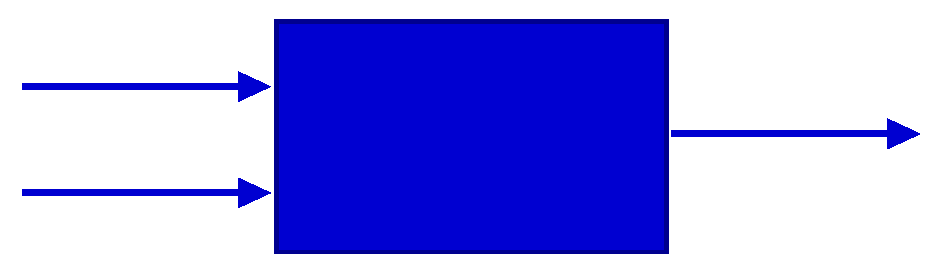
\includegraphics[width=5cm]{kuvat/digi}
\end{center}
Loogisella piirillä on yksi tai useampi sisäänmeno ja
yksi ulostulo. Sisäänmenojen ja ulostulon signaalin arvo
voi olla 1 tai 0. Edellisessä tapauksessa johtimessa on
jännite, jälkimmäisessä tapauksessa ei ole.

Loogiset piirit kootaan loogisista porteista. Seuraavassa
taulukossa on lueteltu loogiset portit, niiden toiminta
ja toimintaa vastaava looginen konnektiivi.

\newpage

\begin{center}
\begin{tabular}{|c|c|c|c|}
\hline
\begin{tabular}{c}
Looginen\\
 portti \\
\end{tabular}
 & Toiminta & Piirrosmerkki & 
\begin{tabular}{c}
Toimintaa \\
vastaava \\
looginen \\
konnektiivi
\end{tabular}
\\ \hline

Tai &
\begin{tabular}{l}
Tai-portti antaa \\
jännitteen, kun ainakin \\
toisessa sisäänmenossa\\ on jännite.
\end{tabular} &
%\begin{center}
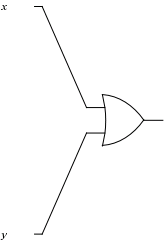
\includegraphics[width=3.5cm]{kuvat/boole/image00}
%\end{center}
&
$A\lor B$
\\ \hline

Ja &
\begin{tabular}{l}
Ja-portti antaa\\ jännitteen vain silloin,\\
kun molemmissa sisään-\\menoissa on jännite.
\end{tabular}
&
%\begin{center}
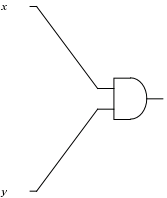
\includegraphics[width=3.5cm]{kuvat/boole/image01}
%\end{center}
&
$A\land B$
\\ \hline

Ei &
\begin{tabular}{l}
Ei-portti antaa\\ jännitteen silloin, kun \\
sisäänmenossa ei ole\\
jännitettä, ja kääntäen. \end{tabular}
&
%\begin{center}
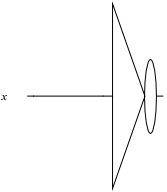
\includegraphics[width=3.5cm]{kuvat/boole/image02}
%\end{center}
&
$\lnot A$
\\ \hline

\end{tabular}

\end{center}

\newpage


Esimerkiksi looginen piiri
\begin{center}
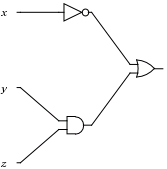
\includegraphics[width=4.5cm]{kuvat/boole/image03}
\end{center}
koostuu kolmesta loogisesta portista ja se vastaa
lausetta $\lnot A\lor (B \land C)$.

%{\bf Tehtäviä}

%\begin{enumerate}
Muodosta seuraavia piirejä vastaavat lauseet.

a)
\begin{center}
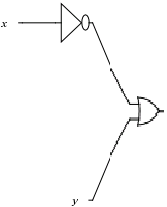
\includegraphics[width=3.5cm]{kuvat/boole/image04}
\end{center}

b)
\begin{center}
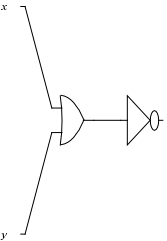
\includegraphics[width=3.5cm]{kuvat/boole/image06}
\end{center}

c)
\begin{center}
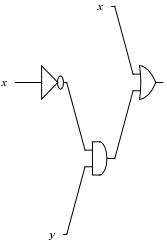
\includegraphics[width=4cm]{kuvat/boole/image05}
\end{center}

d)
\begin{center}
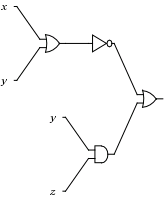
\includegraphics[width=4.5cm]{kuvat/boole/image07}
\end{center}

\item
Piirrä lausetta
a) $\lnot A \land B$ b) $A\lor \lnot (B\land C)$ c)
$(A\land B)\lor (\lnot A \land C)$
vastaava looginen piiri.

\end{enumerate}

{\bf Kotitehtäviä.}

\begin{enumerate}

\item  Kirjoita lauseen negaatio.
\begin{itemize}
\item[a)] $100 > 101$.
\item[b)] Lompakossani on rahaa korkeintaan 10 euroa.
\item[c)] Kaikki ryhmämme opiskelijat ovat Facebookissa.
\item[d)] Koulussamme on täsmälleen kaksi vasenkätistä opettajaa.
\item[e)] En opiskele latinaa enkä kreikkaa.
\item[f)] Maarit pitää lumilautailusta tai käsitöistä muttei molemmista.
\end{itemize}

\item Olkoot lauseet $A$: ''puutarhan portti on auki'', $B$: ''ruusut kukkivat'' ja $C$: ''menen puutarhaan''. Kirjoita suomen kielellä lauseet a) $\lnot A$,  b)  $B\land C$,  c)  $A\lor B$,
d) $\lnot B \land \lnot C$,  e)  $\lnot(A\land B)$  f)  $A \lor \lnot B$,   g)  $(A \land C) \lor (\lnot B \land C)$. 

\item Formalisoi lause.
\begin{itemize}
\item[a)] Kaino ei ole vanha ja Kaino on mies.
\item[b)] Kaino on vanha tai Kaino ei ole mies.
\item[c)] Kaino ei ole vanha mies. 
\item[d)] Kaino ei ole vanha eikä hän ole mies.
\end{itemize}

\item Formalisoi lause.
\begin{itemize}
\item[a)] Amadeus kuuntelee klassista tai Klaus kuuntelee jazzia.
\item[b)] Amadeus ei kuuntele klassista, mutta Klaus kuuntelee jazzia.
\item[c)] Amadeus kuuntelee klassista, mutta Klaus ei kuuntele jazzia, tai sitten Hassinen kuuntelee progea.
\item[d)] Ei ole niin, että Amadeus kuuntelisi klassista, Klaus jazzia ja Hassinen progea.
\end{itemize}

\item 
\begin{itemize}
\item[a)] Laadi totuustaulu lauseille $A\land \lnot A$ ja $A\lor \lnot A$.
\item[b)] Keksi atomilause $A$ ja ilmaise kohdan a) lauseet suomen kielellä.
\end{itemize}

\item
Laadi totuustaulu lauseille a) $\lnot(A\lor B)$,  b)  $\lnot A\land B$,  c) $ (\lnot A\lor B)\land (A\lor \lnot B)$. Millä atomilauseiden $A$ ja  $B$ totuusarvojen yhdistelmillä lauseet ovat tosia?

\item
\begin{itemize}
\item[a)] Laadi totuustaulu lauseelle $A\lor (B\land C)$.  
\item[b)] Laadi totuustaulu lauseelle $(A\lor B)\land C$. 
\item[c)] Vertaa kohtien a) ja b) lauseiden totuusarvoja. Mitä voit päätellä?
\end{itemize}

\item Olkoot lauseet $A$: ''$x\in [-3,1]$'' ja $B$: ''$ x \in [-1,5]$''. Formalisoi lause.
a) $x\in [-3,5]$, b) $x\in [-1,1]$,   c)  $x\in [-3,-1[$  d)  $x\in ]-\infty,-3[$  tai $x\in ]1,\infty[$, 
e) $x\in]-\infty,-3[$  tai $x\in ]5,\infty[$.  

\item Kolme koiranpentua, Alli, Buh ja Caesar ovat epäiltyinä isännän tohvelin repimisestä. Luotettava henkilö, joka puhuu aina totta, antaa seuraavan todistuksen: ''Ei ole totta, että Alli on syyllinen tai Buh ei ole syyllinen. Mutta kuitenkin Alli on syyllinen tai Caesar on syyllinen.'' Käytä atomilauseita $A$: ''Alli on syyllinen'', $B$: ''Buh on syyllinen'' ja $C$: ''Caesar on syyllinen'' ja formalisoi luotettavan henkilön lausunto. Muodosta sille totuustaulu ja päättele, mikä tai mitkä koiranpennuista ovat syyllisiä. 

\item Tutkitaan lausetta ''Suomen kuningas ei ole viiksekäs''. Lause voidaan tulkita ainakin kahdella eri tavalla:
\begin{itemize}
\item[a)] Suomella on kuningas, joka ei ole viiksekäs.
\item[b)] Ei ole niin, että olisi olemassa Suomen viiksekästä kuningasta.
\end{itemize}
Oletetaan, että Suomessa ei ole kuningasta. Onko lause tosi vai epätosi?

\item
Kissoilla lyhyen karvan aiheuttaa dominoiva geeni ja pitkän karvan resessiivinen geeni. Merkitään lyhyen karvan geeniä S ja pitkän karvan geeniä s. Kaikilla nisäkkäillä tiettyyn ominaisuuteen vaikuttaa geenipari, joista toinen geeni on saatu isältä ja toinen emolta. Jos kissan geeneistä ainakin toinen on S, niin se on lyhytkarvainen. Kissa on pitkäkarvainen vain siinä tapauksessa, että se on saanut geenin s molemmilta vanhemmiltaan.  Pentujen emokissa on pitkäkarvainen (ss) ja isäkissa lyhytkarvainen (SS tai Ss). Millaisia pentuja kissat voivat saada, kun isäkissan geenipari on a) SS b) Ss?

\end{enumerate}

\newpage


\subsection{Implikaatio ja ekvivalenssi}
Tässä kappaleessa esitellään kaksi usein käytettyä konnektiivia: {\em implikaatio} eli {\em looginen seuraus} sekä {\em ekvivalenssi} eli {\em looginen yhtäpitävyys}.

\subsection*{Tutkimustehtävä}

\begin{center}
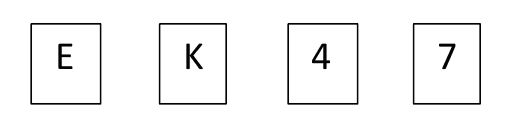
\includegraphics[width=7cm]{kuvat/piaget}
\end{center}

Tarkastellaan oheisen kuvan mukaisia kortteja. Korttien toisella puolella on jokin kirjain ja toisella puolella jokin luku.

1) Ongelmana on selvittää, toteuttavatko kortit seuraavan säännön: Jos kortin toisella puolella on vokaali, niin sen toisella puolella on parillinen luku. Mitkä kortit täytyy vähintään kääntää?

2) Ongelmana on selvittää, toteuttavatko kortit seuraavan säännön: Kortin toisella puolella on parillinen luku, jos ja vain jos sen toisella puolella on vokaali. Mitkä kortit täytyy vähintään kääntää?

Psykologi Jean Piaget (1896 -- 1980) käytti ensimmäistä kysymystä tutkiessaan nuorten ja aikuisten abstraktia ajattelua\\ ({\tt webspace.ship.edu/cgboer/piaget.html}).

{\bf Implikaatio}

Loogista jos $A$ niin $B$ -rakennetta sanotaan implikaatioksi. Implikaatiota merkitään $A\to B$. Implikaatiota  kutsutaan toisinaan loogiseksi seu\-rauk\-sek\-si, mutta tämä ilmaisu on hieman tulkinnanvarainen. Sanalla seuraus on nimittäin puhekielessä kaksi sanan loogisesta merkityksestä poikkeavaa mutta tavallisempaa merkitystä. Seuraus voi tarkoittaa esimerkiksi ajallista seurausta, eli asia tapahtuu toisen jälkeen. Sanalla voidaan myös tarkoittaa kausaalista seurausta, eli asia on toisen aiheuttava syy. Logiikassa ei yleensä kiinnitetä huomiota tällaisiin näkökohtiin. Joskus asiat voivat olla toistensa loogisia seurauksia, vaikka niillä ei olisi kausaalisesti mitään tekemistä toistensa kanssa. Esimerkiksi lause ''jos Caesar elää, niin Helsinki sijaitsee Afrikassa'' on logiikan mielessä tosi. 

Looginen implikaatio $A\to B$  määritellään niin, että se on epätosi ainoastaan tapauksessa, jossa $A$ on tosi mutta $B$ ei ole. Kaikissa muissa tapauksissa se on tosi. Siksi logiikassa usein sanotaan, että epätodesta oletuksesta voi päätellä mitä tahansa.

Esimerkiksi lauseista $A$: ''Anne on suomalainen'' ja $B$: ''Anne on eurooppalainen'' saadaan implikaation avulla lauseet $A \to B$: ''jos Anne on suomalainen, niin hän on eurooppalainen'' sekä myös $B \to A$: ''jos Anne on eurooppalainen, niin hän on suomalainen''. 

Implikaation totuustaulu:

\bigskip

\begin{center}
\begin{tabular}{|c|c|c|}\hline
$A$ & $B$ & $A \to B$ \\ \hline
$1$ & $1$ & $1$\\ %\hline
$1$ & $0$ & $0$\\
$0$ & $1$ & $1$\\
$0$ & $0$ & $1$\\ \hline
\end{tabular}
\end{center}

\bigskip

Kappaleessa \ref{monimloog} osoitetaan, että implikaatiota voidaan ajatella lyhennysmerkintänä lauseelle $\lnot A \lor B$, koska implikaatiolla on sama totuustaulu kuin kyseisellä lauseella.


{\bf Ekvivalenssi.} Jos sekä $A\to B$ että $B\to A$ ovat tosia lauseita, sanotaan, että lauseet $A$ ja $B$ ovat ekvivalentit, $A \lequiv B$. Ekvivalenssia voi ajatella lyhennysmerkintänä lauseelle $(A\to B) \land (B\to A)$. Intuitiivisesti se tarkoittaa lauseiden $A$ ja $B$ yhtäpitävyyttä (vrt. yhtäsuuruus), eli molemmat lauseet saavat samat totuusarvot.

Esimerkiksi lauseiden $A$: ''Pekka menee hammaslääkäriin'' ja $B$: ''Pekan hammasta särkee'' ekvivalenssi on $A \lequiv B$: ''Pekka menee hammaslääkäriin, jos ja vain jos hänen hammastaan särkee''.

Ekvivalenssin totuustaulu:

\bigskip

\begin{center}
\begin{tabular}{|c|c|c|}\hline
$A$ & $B$ & $A \lequiv  B$ \\ \hline
$1$ & $1$ & $1$\\ %\hline
$1$ & $0$ & $0$\\
$0$ & $1$ & $0$\\
$0$ & $0$ & $1$\\ \hline
\end{tabular}
\end{center}

\bigskip

Ekvivalenssi $A\lequiv B$ voidaan lukea ''$A$, jos ja vain jos $B$''. Tämä ilmaisu esiintyy usein matemaattisessa tekstissä. Voidaan käyttää myös esimerkiksi ilmaisuja ''$A$ silloin ja vain silloin, kun $B$'' ja ''$A$ ja $B$ ovat yhtäpitävät''.

{\bf Esimerkki 1.} Formalisoi lause. Missä tilanteissa lause on tosi? a) On kesä, ja jos on kesä, järvivesi on lämmintä. b) Uin silloin ja vain silloin, kun on kesä ja järvivesi on lämmintä. 

{\bf Ratkaisu:}
Käytetään atomilauseita $A$: ''on kesä'',
$B$: ''järvivesi on lämmintä'' ja $C$: ''uin''.
\begin{itemize}
\item[a)] Lause on $A \land (A \to B)$. Muodostetaan
lauseen totuustaulu.

\begin{center}
\begin{tabular}{|c|c|c|c|}\hline
$A$ & $B$ & $A \to B$ & $A \land (A \to B)$\\ \hline
$1$ & $1$ & $1$ & $1$\\ %\hline
$1$ & $0$ & $0$ & $0$\\
$0$ & $1$ & $1$ & $0$\\
$0$ & $0$ & $1$ & $0$\\ \hline
\end{tabular}
\end{center}

Lause on tosi täsmälleen silloin, kun $A$ ja $B$ ovat
molemmat tosia eli kun on kesä ja järvivesi on lämmintä.
\item[b)] Lause on $C \lequiv (A \land B)$. Muodostetaan
lauseen totuustaulu.

\begin{center}
\begin{tabular}{|c|c|c|c|c|c|}\hline
$A$ & $B$ & $C$ & $A \land B$ & $C \lequiv (A \land B)$\\
\hline
$1$ & $1$ & $1$ & $1$ & $1$\\ %\hline
$1$ & $1$ & $0$ & $1$ & $0$\\
$1$ & $0$ & $1$ & $0$ & $0$\\ %\hline
$1$ & $0$ & $0$ & $0$ & $1$\\
$0$ & $1$ & $1$ & $0$ & $0$\\
$0$ & $1$ & $0$ & $0$ & $1$\\ %\hline
$0$ & $0$ & $1$ & $0$ & $0$\\
$0$ & $0$ & $0$ & $0$ & $1$\\ \hline
\end{tabular}
\end{center}

Lause on tosi, kun atomilauseet $A$, $B$ ja $C$ ovat
kaikki tosia, kun $A$ on tosi sekä $B$ ja $C$ ovat
epätosia, kun $B$ on tosi sekä $A$ ja $C$ ovat epätosia
tai kun kaikki atomilauseet ovat epätosia. Tämä vastaa
seuraavia tilanteita: on kesä, järvivesi on lämmintä ja
uin; on kesä, järvivesi ei ole lämmintä enkä ui; ei ole
kesä, järvivesi on lämmintä, mutta en ui; ei ole kesä,
järvivesi ei ole lämmintä enkä ui.
\end{itemize}

{\bf Vastaus: } a) Lause on tosi, kun on kesä ja järvivesi on lämmintä.

b) Lause on tosi seuraavissa tilanteissa: on kesä, järvivesi on lämmintä 
ja uin; on kesä, järvivesi ei ole lämmintä enkä ui; ei ole 
kesä, järvivesi on lämmintä, mutta en ui; ei ole kesä, 
järvivesi ei ole lämmintä enkä ui.

{\bf Esimerkki 2.}
Matti, Seppo ja Teppo ovat epäiltyinä rikoksesta. Heitä kuulusteleva konstaapeli Reinikainen tietää, että syytön puhuu aina totta ja syyllinen valehtelee aina.

Matti sanoi: ''Jos Seppo on syytön, niin minäkin olen.''

Seppo väitti: ''Minä olen syytön, jos ja vain jos Teppo on syytön.''

Teppo sanoi: ''Seppo yksin on syyllinen.'' 

Ratkaise totuustaulun avulla, kuka tai ketkä ovat syyllisiä.

{\bf Ratkaisu:} Tarkastellaan lauseita $M$: ''Matti on syytön'', $S$: ''Seppo on syytön'' ja $T$: ''Teppo on syytön''.

Matin, Sepon ja Tepon väitteet formalisoituina ovat $S\to M$, $S\lequiv T$
ja $M\land \lnot S \land T$. Tutkitaan, kuinka väitteet riippuvat lauseiden $M$, $S$ ja $T$ totuusarvoista. Muodostetaan totuustaulu:

\bigskip

\begin{center}
\begin{tabular}{|c|c|c|c|c|c|c|c|}\hline
$M$ & $S$ & $T$ & $S\to M$ & $S\lequiv T$ & $\lnot S$ & $M\land \lnot S$ & $M\land \lnot S \land T$\\ \hline
$1$ & $1$ & $1$ & $1$ & $1$ & $0$ & $0$ & $0$\\ %\hline
$1$ & $1$ & $0$ & $1$ & $0$ & $0$ & $0$ & $0$\\
$1$ & $0$ & $1$ & $1$ & $0$ & $1$ & $1$ & $1$\\
$1$ & $0$ & $0$ & $1$ & $1$ & $1$ & $1$ & $0$\\
$0$ & $1$ & $1$ & $0$ & $1$ & $0$ & $0$ & $0$\\
$0$ & $1$ & $0$ & $0$ & $0$ & $0$ & $0$ & $0$\\
$0$ & $0$ & $1$ & $1$ & $0$ & $1$ & $0$ & $0$\\
$0$ & $0$ & $0$ & $1$ & $1$ & $1$ & $0$ & $0$ \\ \hline
\end{tabular}
\end{center}

\bigskip

Koska syytön puhuu totta ja syyllinen valehtelee, on löydettävä totuustaulusta rivi, jolla väitteillä $S\to M$, $S\lequiv T$ ja $M \land \lnot S\land T$ on samat totuusarvot kuin lauseilla $M$, $S$ ja $T$. Tällainen rivi on totuustaulun kolmas rivi. Siten Seppo on yksin syyllinen.

{\bf Vastaus:} Seppo on yksin syyllinen.

\bigskip

{\bf Konnektiivien suoritusjärjestys.} 
Loogisten lauseiden lukeminen helpottuu ja tarve sulkeiden käyttämiseen vähenee, jos sovitaan konnektiivien suoritusjärjestyksestä. Nykyään yleisimmin käytetään seuraavaa suoritusjärjestystä, jota noudatetaan myös tässä kirjassa: $\lnot$, $\land$, $\lor$, $\to$, $\lequiv$, ja vasemmalta oikealle.

Suoritusjärjestystä voidaan muuttaa käyttämällä sulkeita. Sulkeita kannattaa myös käyttää aina silloin, kun se helpottaa loogisen lauseen lukemista.

{\bf Esimerkki 3.}
Mikä on lauseiden a) $B \lequiv \lnot A\lor B \land A \to B$, ja  b)  $(B\lequiv \lnot A)\lor B \land (A\to B)$  totuusarvo, kun $A$ on tosi ja $B$ epätosi?   

{\bf Ratkaisu:}

%\begin{itemize}
%\item[a)]

a) Muodostetaan totuustaulu:

\begin{center}
\begin{tabular}{|c|c|c|c|c|c|c|}\hline
$A$ & $B$ & $\lnot A$ & $B \land A $ & $\lnot A\lor B \land A$ & $\lnot A\lor B \land A \to B$ & $B \lequiv \lnot A\lor B \land A \to B$\\ \hline
$1$ & $0$ & $0$ & $0$ & $0$ & $1$ & $0$\\ \hline
\end{tabular}
\end{center}

Ensin suoritetaan negaatio. Sen jälkeen tulevat konjunktio ja disjunktio. Implikaatio 	suoritetaan ennen ekvivalenssia. 	Kun $A$ on tosi ja $B$ epätosi, lause on epätosi.

%\item[b)]

b) Muodostetaan totuustaulu:

\begin{center}
\begin{tabular}{|c|c|c|c|c|c|c|}\hline
$A$ & $B$ & $\lnot A$ & $B\lequiv \lnot A$ & $A\to B$ & $B \land (A\to B)$ &  $(B\lequiv \lnot A)\lor B \land (A\to B)$\\ \hline
$1$ & $0$ & $0$ & $1$ & $0$ & $0$ & $1$\\ \hline
\end{tabular}
\end{center}

Ensin suoritetaan negaatio. Sen jälkeen tulevat sulkeissa olevat ekvivalenssi ja implikaatio. Konjunktio suoritetaan ennen disjunktiota. Kun $A$ on tosi ja $B$ epätosi, lause on tosi.

{\bf Vastaus:} a) epätosi, b) tosi

{\bf Harvinaisempia konnektiiveja (Lisämateriaalia).} Logiikassa ja tietotekniikassa esiintyy myös muita, harvinaisempia loogisia konnektiiveja. Esimerkki tällaisesta on {\em poissulkeva tai} (engl. exclusive or), josta usein käytetään tietotekniikasta tulevaa lyhennettä {\em xor}. Poissulkevan tain totuustaulu on seuraava:

\bigskip

\begin{center}
\begin{tabular}{|c|c|c|}\hline
$A$ & $B$ & $A\,\mathrm{xor}\,B$ \\ \hline
$1$ & $1$ & $0$\\ %\hline
$1$ & $0$ & $1$\\
$0$ & $1$ & $1$\\
$0$ & $0$ & $0$\\ \hline
\end{tabular}
\end{center}

\bigskip

Kuten kappaleessa \ref{konnektiivit} todettiin, arkikielessä sana tai saattaa tarkoittaa asiayhteydestä riippuen joskus poissulkevaa tai-operaatiota ja toisinaan loogista disjunktiota.

Lisää loogisia konnektiiveja esitellään harjoitustehtävissä.


\newpage

%\bigskip

\subsection*{Tehtäviä}

\begin{enumerate}
\item Olkoot $A$: ''Matti on insinööri'' ja $B$: ''Matilla on hyvä työpaikka''.
Suomenna lause.
\begin{itemize}
\item[a)] $A\land B$,
\item[b)] $\lnot A \lor B$,
\item[c)] $A\to B$,
\item[d)] $\lnot B\to A$,
\item[e)] $\lnot( B \to A )$.
\item[f)] $ B \lequiv A$.
\end{itemize}

\item Olkoot $A$: ''Liisa on lomalla'' ja $B$: ''Liisa on iloinen''. Formalisoi lauseet:
\begin{itemize}
\item[a)] Jos Liisa on lomalla, hän on iloinen.
\item[b)] Liisa on lomalla, mutta hän ei ole iloinen.
\item[c)] Liisa on iloinen silloin ja vain silloin, kun hän on lomalla.
\item[d)] Jos Liisa ei ole iloinen, hän ei ole lomalla.
\end{itemize}

\item Onko lause tosi?
\begin{itemize}
\item[a)] Jos Tallinna on Norjan pääkaupunki, niin Tukholma on Ruotsin pääkaupunki.
\item[b)] Jos Tallinna on Norjan pääkaupunki, niin Budapest on Ruotsin pääkaupunki.
\item[c)] Jos Leonardo da Vinci on kuollut, niin Aleksis Kivi on saksalainen ralliautoilija.
\item[d)] Jos Leonardo da Vinci on kuollut, niin Leo Tolstoi on venäläinen kirjailija.
\end{itemize}

\item Laadi lauseen totuustaulu.
\begin{itemize}
\item[a)] $\lnot A \to B$
\item[b)] $A\lequiv \lnot B$
\item[c)] $\lnot( A\land B )\to A$
\end{itemize}

\item Laadi lauseen totuustaulu.
\begin{itemize}
\item[a)] $\lnot A \lor B \to C \land A$
\item[b)] $( A\to B ) \lequiv (C\to B)$
\end{itemize}

\item Formalisoi lause. Missä tilanteissa lause on tosi?
\begin{itemize}
\item[a)]
Jos mustikat polun varrella eivät ole kypsiä, niin polulla vaeltaminen on turvallista.
\item[b)] Jos mustikat polun varrella ovat kypsiä, niin silloin polulla vaeltaminen on turvallista, jos ja vain jos karhuja ei ole nähty alueella. 
\item[c)] Polulla vaeltaminen on turvallista silloin ja vain silloin, kun mustikat eivät ole kypsiä tai alueella ei ole nähty karhuja.
\end{itemize}

\item Formalisoi lause ja laadi lauseen totuustaulu. Mitä huomaat? Kertooko lause mitään siitä, onko logiikan opiskelu oikeasti hauskaa juuri tällä hetkellä? 
\begin{itemize}
\item[a)] Jos sataa ja ei sada, niin logiikan opiskelu on hauskaa.
\item[b)] Jos sataa ja ei sada, niin logiikan opiskelu ei ole hauskaa.
\end{itemize}

\item Perheen lapsia Annaa ja Markusta epäillään kaappiin piilotetun suklaalevyn katoamisesta. Luotettava todistaja kertoo tiedot:
Anna on syyllinen tai Markus on syyllinen.
Anna on syytön tai Markus on syytön. 
Jos Anna on syyllinen, niin Markus on syyllinen.

Kumpi lapsista on käynyt suklaavarkaissa?

\item Edwards, Petterson ja Smith ovat syytettyinä omenavarkaudesta. Neiti Marble kuulustelee heitä. Edwards sanoo: ''Jos Petterson on syytön, niin minä olen syyllinen.'' Petterson toteaa: ''Minä olen syyllinen, jos ja vain jos Edwards on syyllinen.'' Smith väittää: ''Olemme kaikki syyttömiä.'' Neiti Marble tietää, että syylliset valehtelevat aina ja syyttömät puhuvat aina totta. Ratkaise totuustaulun avulla, kuka tai ketkä syytetyistä ovat käyneet omenavarkaissa.

\item Eräässä maassa kaikki kuuluvat joko hattujen tai myssyjen puolueeseen. Hatut valehtelevat aina ja myssyt puhuvat aina totta. Kolme kansalaista keskusteli keskenään. Heidän joukossaan saattoi olla vieraan puolueen vakoilija. Arthur sanoi, että Claus on myssy. Berit totesi, että Arthur on myssy ja myös hän itse on myssy. Claus väitti, että jos Arthur on hattu, niin myös hän itse on hattu. Tutki totuustaulun avulla, kuka oli mahdollinen vakoilija.

\item Olkoot lauseet $A$: ''herään ajoissa'', $B$: ''menen kouluun'' ja $C$: ''opiskelen logiikkaa''.
Esitä sanoin lause $A \to B \lor C$. Onko lauseen tulkinta $A \to (B \lor C)$ vai $(A \to B) \lor C$? Miten tulkinnat eroavat toisistaan? 

\item
Vertaa lauseiden totuusarvoja atomilauseiden $A$, $B$ ja $C$ eri totuusarvoilla. Onko sulkeiden muuttamisella vaikutusta lauseen totuusarvoon?
\begin{itemize}
\item[a)] $(A\to B)\to C$ ja $A\to (B\to C)$.
\item[b)] $(A\land B)\land C$ ja $A\land (B\land C)$.
\end{itemize}

\item (Lisämateriaalia)  Tietokoneet käsittelevät tietoa käyttäen bittejä. Bitillä on kaksi mahdollista arvoa, $0$ ja $1$.
Bittijono on jono, jossa on yksi tai useampia bittejä. Esimerkiksi $1001\, 0010$ on bittijono, jonka pituus on $8$ bittiä. Samanpituisille bittijonoille määritellään bittikohtaiset tai, ja sekä poissulkeva tai (or, and sekä xor). Esimerkiksi bittijonojen $1100$ ja $1010$ bittikohtainen tai on jono $1110$, bittikohtainen ja on jono $1000$ sekä bittikohtainen poissulkeva tai on jono $0110$. Muodosta a) bittikohtainen tai  b) bittikohtainen ja c) bittikohtainen poissulkeva tai jonoille $1111\, 0000$ ja $1010\, 1010$.

\item (Lisämateriaalia)  Muodosta bittijono a)  $(0\, 1111 \land 1\, 0101) \lor 0\, 1000$  b) $(0\, 1010 \xor 1\, 1011) \xor 0\, 1001$. 

\end{enumerate}

{\bf Kotitehtäviä.}

\begin{enumerate}

\item
Olkoot $A$: ''Timo opiskelee matematiikkaa'', $B$: ''Timo osallistuu logiikan kurssille'' ja $C$: ''Timo opiskelee filosofiaa''. Suomenna lause.
\begin{itemize}
\item[a)] $\lnot A \to \lnot B$.
\item[b)] $A\lequiv B$.
\item[c)] $A\lor C \to B$.
\item[d)] $C\lequiv (B\to \lnot A)$.
\end{itemize}

\item Onko lause tosi?
\begin{itemize}
\item[a)] Jos $(-2)^3= -8$, niin $(-2)^3= -8$.
\item[b)] Jos $(-2)^3= -8$, niin $(-2)^3=  8$.
\item[c)] Jos luku $8$ on pariton, niin luku $8$ on pariton.
\item[d)] Jos luku $8$ on pariton, niin luku $8$ on parillinen.
\end{itemize}

\item
Formalisoi lause.
\begin{itemize}
\item[a)] Jos opettaja on pirteä, niin televisiosta ei ole tullut illalla jalkapalloa.
\item[b)] Suomi voittaa jalkapallon maailmanmestaruuden silloin ja vain silloin, kun lehmät lentävät ja vaaleanpunaiset norsut kävelevät kadulla.
\item[c)] En seuraa jalkapalloa eikä Suomen maajoukkue menesty. 
\item[d)] Jos ottelu ei pääty tasapeliin, niin joko kotijoukkue tai vierasjoukkue voittaa pelin.
\end{itemize}

\item Laadi lauseen totuustaulu.
\begin{itemize}
\item[a)] $A\land B\to \lnot B$
\item[b)] $(A\lequiv B)\land B\to C\lor A$
\item[c)] $(\lnot A\to B)\lequiv (C\to B\land A)$
\end{itemize}


\item
Olkoot $A$: ''Timo opiskelee matematiikkaa'', $B$: ''Timo osallistuu logiikan kurssille'' ja $C$: ''Timo opiskelee filosofiaa''. Formalisoi lause. Missä tilanteissa lause on tosi?
\begin{itemize}
\item[a)] Timo opiskelee matematiikkaa ja filosofiaa.
\item[b)] Jos Timo opiskelee matematiikkaa, hän osallistuu logiikan kurssille.
\item[c)] Timo osallistuu logiikan kurssille silloin ja vain silloin, kun hän opiskelee filosofiaa tai matematiikkaa.
\item[d)] Jos Timo osallistuu logiikan kurssille, opiskelee hän joko matematiikka tai filosofiaa, muttei molempia.
\end{itemize}


\item Poliisit Mauno ja Martti saavat kiinni rikoksesta epäilemänsä Jaskan. Tiedetään, että Jaska ei koskaan valehtele. Mauno toteaa Martille: ''Jos Jaska on syyllinen, on hänellä ollut rikostoveri.'' Jaska vastaa: ''Tuo ei ole totta!'' Tähän Martti tokaisee: ''Sehän tunnusti helpolla!'' Tutki Maunon lausetta ja osoita Martin johtopäätös oikeaksi.

\item Mattia, Seppoa ja Teppoa epäillään polkupyörävarkaudesta. Konstaapeli Reinikainen tietää, että syytön puhuu aina totta ja syyllinen valehtelee aina. Reinikainen kuulustelee kolmea epäiltyä. Matti sanoo: ''Teppo on syyllinen.'' Seppo väittää: ''Matti on syyllinen tai Teppo valehtelee.'' Teppo toteaa: ''Seppo on syyllinen.'' Ratkaise totuustaulun avulla, kuka on syyllinen. 

\item Helinä, Heljä ja Helena asuvat samassa talossa. Epäillään, että loton päävoitto on osunut taloon. Luotettavalta taholta on tullut tietoja:

Jos Heljä on voittaja, niin Helinäkin on. 
Heljä on voittaja, jos ja vain jos Helena on voittaja.
Ainakin yksi naisista on voittaja, mutta kaikki eivät ole.

Kuka tai ketkä ovat voittaneet lotossa?

\item
Mitä eroa on seuraavissa ehdoissa?
\begin{enumerate}
\item Henkilö saa työpaikan matkamuistomyymälässä, jos hänellä on kokemusta kassakoneen käytöstä.
\item Matkamuistomyymälässä työskentelevältä edellytetään kokemusta kassakoneen käytöstä.
\item 
Henkilö saa työpaikan matkamuistomyymälässä silloin ja vain silloin, kun hänellä on kokemusta kassakoneen käytöstä.
\end{enumerate}


\item

Vertaa lauseiden totuusarvoja atomilauseiden $A$, $B$ ja $C$ eri totuusarvoilla. Onko sulkeiden muuttamisella vaikutusta lauseen totuusarvoon?

\begin{itemize}

\item[a)] $(A\lor B)\lor C$ ja $A\lor (B\lor C)$.

\item[b)] $(A\lequiv B)\lequiv C$ ja $A\lequiv (B\lequiv C)$.

\item[c)] $\lnot A \lequiv (B \land C)$ ja $\lnot (A \lequiv B) \land C$.

\end{itemize}

%\item Muodosta
%\begin{itemize}
%\item[a)] lauseen $A$ ja lauseen $B$ negaation konjunktio,
%\item[b)] lauseiden $A$ ja $B$ disjunktion negaatio,
%\item[c)] lauseen $A$ negaation ekvivalenssi lauseiden $B$ ja $C$ konjunktion kanssa.
%\end{itemize}

\item
Olkoon $v$ sellainen funktio, että $v(A) = 1$, jos lause $A$ on tosi, ja $v(A) = 0$, jos lause $A$ on epätosi. Osoita, että yhtälö pätee kaikilla lauseiden $A$ ja $B$ totuusarvojen yhdistelmillä.

\begin{itemize}
\item[a)] $v(A\land B)=v(A)v(B)$,
\item[b)] $v(A\lor B)=v(A)+v(B)- v(A)v(B)$,
\item[c)] $v(A\to B)=1-v(A)(1-v(B))$.
\end{itemize}

\item
Peircen nuoli on konnektiivi, joka luonnollisessa kielessä tarkoittaa samaa kuin ''ei $A$ eikä $B$''. Shefferin viiva on konnektiivi, joka luonnollisessa kielessä tarkoittaa samaa kuin ''ei molemmat $A$ ja $B$''. Laadi näiden konnektiivien totuustaulut. 
\end{enumerate}

\newpage

\subsection{Monimutkaisempia loogisia rakenteita}
\label{monimloog}
Seuraavaksi tarkastellaan eräitä usein esiintyviä loogisia rakenteita. Tällaisia rakenteita ovat {\em tautologiat}, {\em loogisesti ekvivalentit} ja {\em ristiriitaiset lauseet}. On tärkeää oppia tunnistamaan nämä rakenteet, koska niitä käytetään usein logiikan yhteydessä.

\subsection*{Tutkimustehtävä}
Turisti tapasi kaksi saarelaista, Hipsun ja Vipsun. Hän kyseli heiltä, kuinka hyvin kala syö, ja sai seuraavat vastaukset.
\begin{enumerate}
\item[a)] On pilvistä, tai sitten jos kala ei syö, niin ei ole pilvistä.
\item[b)] On pilvistä tai kala syö, mutta ei ole pilvistä eikä kala syö.
\end{enumerate}
Formalisoi lauseet käyttäen atomilauseita $P$: ''on pilvistä'' ja $K$: ''kala syö''. Tutki totuustaulun avulla, milloin väitteet ovat tosia. Mitä huomaat?

{\bf Tautologia.}
Tautologialla tarkoitetaan lausetta, joka on tosi riippumatta asioiden tilasta. Tällainen lause on esimerkiksi: ''Huominen on aina tulevaisuutta.'' Sanaa tautologia käytetään filosofiassa myös argumenteista, joita ei voi kumota tekemättä ristiriitaisia oletuksia.

{\bf Esimerkki 1.} Osoita, että lause $(A\land B)\lor (\lnot A \lor \lnot B)$ on
tautologia.

{\bf Ratkaisu:}
Muodostetaan lauseen $(A\land B)\lor (\lnot A \lor \lnot
B)$ totuustaulu:

\begin{center}
\begin{tabular}{|c|c|c|c|c|c|c|}\hline
$A$ & $B$ & $A\land B$ & $\lnot A$ & $\lnot B$ & $ \lnot
A \lor \lnot B $ & $(A\land B)\lor (\lnot A \lor \lnot B)$
\\ \hline
$1$ & $1$ & $1$ & $0$ & $0$ & $0$ & $1$ \\ %\hline
$1$ & $0$ & $0$ & $0$ & $1$ & $1$ & $1$ \\
$0$ & $1$ & $0$ & $1$ & $0$ & $1$ & $1$ \\
$0$ & $0$ & $0$ & $1$ & $1$ & $1$ & $1$ \\ \hline
\end{tabular}
\end{center}

Koska lause on aina tosi, se on tautologia.

{\bf Looginen ekvivalenssi.}  Loogisesti
ekvivalentit lauseet saavat samat totuusarvot
kaikissa tilanteissa. Kaksi lausetta $L_1$ ja
$L_2$ ovat siis  loogisesti ekvivalentteja, jos niillä
on samat totuustaulut. Toisin sanoen lause $L_1 \lequiv L_2$ on tautologia.

{\bf Esimerkki 2.} Osoita, että lauseet $A\to B$ ja $\lnot A \lor B$ ovat loogisesti
ekvivalentit.

{\bf Ratkaisu:}
Verrataan lauseiden $A\to B$ ja $\lnot A \lor B$
totuustauluja: 

\begin{center}
\begin{tabular}{|c|c|c|c|c|}\hline
$A$ & $B$ & $A\to B$ & $\lnot A$ & $\lnot A\lor B$ \\ \hline
$1$ & $1$ & $1$ & $0$ & $1$  \\ %\hline
$1$ & $0$ & $0$ & $0$ & $0$  \\
$0$ & $1$ & $1$ & $1$ & $1$  \\
$0$ & $0$ & $1$ & $1$ & $1$  \\ \hline
\end{tabular}
\end{center}

Koska lauseiden $A\to B$ ja $\lnot A \lor B$ totuusarvot
ovat aina samat, lauseet ovat loogisesti ekvivalentit.

{\em Kolmannen poissulkevan laki} sanoo, että kaikki lauseet ovat joko tosia tai epätosia. Formaalilla kielellä kolmannen poissulkevan laki tarkoittaa, että lause $A \lor \lnot A$ on tautologia. Tämä voidaan nähdä seuraavasta totuustaulusta:

\bigskip

\begin{center}
\begin{tabular}{|c|c|c|}\hline
$A$ & $\lnot A$ & $A \lor  \lnot A$ \\ \hline
$1$ & $0$ & $1$\\
$0$ & $1$ & $1$\\ \hline
\end{tabular}
\end{center}

\bigskip


{\bf Moniarvoiset logiikat (lisämateriaalia).}
Lauseen $A \lor \lnot A$ tautologisuus liittyy klassisen logiikan kaksiarvoisuuteen. Voidaan ajatella myös sellaisia päättelymalleja, joissa lause $A \lor \lnot A$ ei ole tautologia. Esimerkki tällaisesta on {\em kolmiarvoinen logiikka}, jossa mahdollisia totuusarvoja ovat tosi, epätosi ja epävarma.  Toinen esimerkki on niin kutsuttu {\em sumean logiikka}, jossa on äärettömän monta totuusarvoa. Erilaiset päättelyjärjestelmät eivät kuitenkaan kumoa toisiaan, vaan logiikkaa sovellettaessa käytetään kuhunkin tilanteeseen sopivaa päättelyjärjestelmää. Esimerkiksi kolmiarvoinen logiikka soveltuu tilanteisiin, joissa käytössä oleva informaatio ajatellaan epätäydelliseksi.

{\bf Ristiriitainen lause.}
Lausetta, joka ei toteudu missään tilanteessa, kutsutaan loogisesti ristiriitaiseksi. Lauseen ristiriitaisuutta voidaan jälleen tutkia totuustaulun avulla. Loogisesti ristiriitaisen lauseen negaatio on tautologia. 

Yksinkertaisin esimerkki ristiriitaisesta lauseesta on lause $A\land \lnot A$. Sen totuustaulu on seuraava:

\bigskip

\begin{center}
\begin{tabular}{|c|c|c|}\hline
$A$ & $\lnot A$ & $A \land  \lnot A$ \\ \hline
$1$ & $0$ & $0$\\
$0$ & $1$ & $0$\\ \hline
\end{tabular}
\end{center}

\bigskip


{\bf Päättelysääntöjä.} Logiikassa esiintyy monia hyödyllisiksi havaittuja päättelysääntöjä, joille on annettu nimi. Nämä päättelysäännöt ovat esimerkkejä tautologioista, ja niiden tautologisuus voidaan osoittaa esimerkiksi totuustaulua käyttämällä.

Tärkeitä päättelysääntöjä ovat esimerkiksi {\em De Morganin lait}
\[
\lnot(A \land B) \lequiv \lnot A \lor \lnot B
\]
ja
\[
\lnot(A \lor B) \lequiv \lnot A \land \lnot B,
\]
jotka liittävät toisiinsa loogiset ja- sekä tai-konnektiivit.
%{\bf de Morganin lait.}

{\em Kaksoisnegaation laki} sanoo, että lauseen $A$ kaksinkertainen negaatio $\lnot \lnot A$ on loogisesti ekvivalentti lauseen $A$ kanssa:
\[
\lnot \lnot A \lequiv A.
\]
{\em Kontraposition laki} puolestaan sanoo, että lauseet $A\to B$ ja $\lnot B \to \lnot A$ ovat loogisesti ekvivalentit. Tämän voi osoittaa paitsi totuustauluja käyttämällä myös soveltamalla De Morganin lakeja.
Matematiikassa tärkeä todistusmenetelmä, niin sanottu käänteinen todistus, perustuu kontraposition lakiin. Käänteistä todistusta käsitellään luvussa 4.

%	{\bf Laita perustelu esimerkiksi. Myös mieti mahdollista viittausta käänteiseen todistukseen (Antti/AM).}
%kk(käytä muotoilua lauseet ... ovat loogisesti ekvivalentit).

Seuraavaan taulukkoon on koottu edellisten lisäksi muutamia muita tunnetuimpia päättelysääntöjä: %***********

\begin{tabular}{|l|c|}
\hline
{\bf Päättelysääntöjä} & \\\hline
{\em De Morganin 1. laki} & $\lnot(A \land B) \lequiv \lnot A \lor \lnot B$\\\hline
{\em De Morganin 2. laki} & $\lnot(A \lor B) \lequiv \lnot A \land \lnot B$\\\hline
{\em Kaksoisnegaation laki} & $\lnot \lnot A \lequiv A$\\\hline
{\em Kontraposition laki} & $(A\to B)\lequiv (\lnot B \to \lnot A)$\\\hline
{\em Modus ponens} & $(A\land (A\to B)) \to B$ \\\hline
{\em Modus tollens} & $((A\to B) \land \lnot B) \to \lnot A$ \\\hline
{\em Reductio ad absurdum} & $(\lnot A \to (B \land \lnot B))\to A$\\\hline
\end{tabular}

{\bf Esimerkki 3.}
Esitä  sanallinen muotoilu a) De Morganin 1. laille
\[
\lnot (A\land B) \lequiv \lnot A \lor \lnot B,
\]
b) modus tollens -päättelysäännölle
\[
((A\to B)\land \lnot B) \to \lnot A.
\]

{\bf Ratkaisu:}

a) Jos $A$ ja $B$ ei ole tosi, niin $A$ ei ole tosi tai $B$ ei ole tosi. Jos $A$ ei ole tosi tai $B$ ei ole tosi, niin $A$ ja $B$ ei ole tosi.

b) Jos $B$ on $A$:n looginen seuraus ja $B$ ei ole tosi, niin $A$ ei ole tosi.

{\bf Esimerkki 4.}
Osoita kontraposition laki oikeaksi totuustaulun avulla.

{\bf Ratkaisu:} 
Muodostetaan totuustaulu lauseille  $A\to B$  ja  $\lnot B \to \lnot A$.

\bigskip

\begin{center}
\begin{tabular}{|c|c|c|c|c|c|}\hline
$A$ & $B$ &  $A\to B$ & $\lnot A$  & $\lnot B$ & $\lnot B \to \lnot A$ \\ \hline
$1$ & $1$ & $1$ & $0$ & $0$ & $1$\\ 
$1$ & $0$ & $0$ & $0$ & $1$ & $0$\\
$0$ & $1$ & $1$ & $1$ & $0$ & $1$\\
$0$ & $0$ & $1$ & $1$ & $1$ & $1$\\ \hline
\end{tabular}
\end{center}

\bigskip

Koska lauseiden $A\to B$ ja $\lnot B \to \lnot A$ totuusarvot ovat samat kaikilla atomilauseiden $A$ ja $B$ totuusarvoilla, lauseet ovat loogisesti ekvivalentit.


{\bf Esimerkki 5.} 
Osoita ilman totuustauluja, että lauseet  a) $\lnot(A \land \lnot B)$  ja  $\lnot A \lor B$,    b)  
$\lnot C\to A \lor B$ ja $\lnot A \land \lnot B \to C$ ovat loogisesti ekvivalentit.

{\bf Ratkaisu:}
Logiikan päättelysääntöjen avulla voidaan muodostaa uusia, alkuperäisen lauseen kanssa loogisesti ekvivalentteja lauseita.

a)

\begin{tabular}{ll}
$\lnot (A \land \lnot B)$ & De Morganin laki \\
$\lnot A \lor \lnot (\lnot B)$ & kaksoisnegaation laki \\
$\lnot A \lor B$ & \\
\end{tabular}

Lauseet $\lnot(A \land \lnot B)$  ja  $\lnot A \lor B$ ovat loogisesti ekvivalentit.

b)

\begin{tabular}{ll}
$\lnot C \to A \lor B$ & kontraposition laki \\
$\lnot (A\lor B)\to \lnot(\lnot C)$ & kaksoisnegaation laki \\
$\lnot (A \lor B) \to C$ & De Morganin laki\\
$\lnot A \land \lnot B \to C$
\end{tabular}

Lauseet $\lnot C\to A \lor B$ ja $\lnot A \land \lnot B \to C$ ovat loogisesti ekvivalentit.

%\bigskip

\newpage


\subsection*{Tehtäviä}

\begin{enumerate}
\item Tutki, onko lause tautologia.
\begin{itemize}
\item[a)] $A\lor \lnot A$,
\item[b)] $A \land \lnot A$,
\item[c)] $A \to B \lor A$,
\item[d)] $A \to B \land A$,
\end{itemize}

\item Osoita lause tautologiaksi.
\begin{itemize}
\item[a)] $A\to B\land \lnot B \lequiv \lnot A$.
\item[b)] $(A\to B) \land (B\to C)\to (A\to C)$.
\end{itemize}

\item Olkoot $A$: ''kello soi'' ja $B$: ''tunti loppuu''.
Kirjoita luonnollisella kielellä lauseet $A\to B$ ja
$\lnot(A \land \lnot B )$. Tarkoittavatko ne samaa?

\item Osoita lauseet loogisesti ekvivalenteiksi
totuustaulujen avulla.
\begin{itemize}
\item[a)] $A\land B$ ja $\lnot(\lnot A\lor \lnot B )$.
\item[b)] $A\lequiv B$ ja $(A\to B)\land (B \to A)$.
\item[c)] $A\lequiv B$ ja $(A\land B) \lor (\lnot A\land
\lnot B )$.
\end{itemize}

\item Osoita vaihdantalait
\begin{itemize}
\item[a)]
\[
A \land B \lequiv B \land A,
\]
\item[b)]
\[
A \lor B \lequiv B \lor A
\]
\end{itemize}
oikeaksi totuustaulujen avulla.

\item Muodosta atomilauseista $A$ ja $B$ lause, joka on
loogisesti ekvivalentti lauseen $X$ kanssa.
\begin{center}
\begin{tabular}{|c|c|c|}\hline
$A$ & $B$ & $X$\\ \hline
$1$ & $1$ & $0$\\
$1$ & $0$ & $1$\\
$0$ & $1$ & $1$\\
$0$ & $0$ & $1$\\ \hline
\end{tabular}
\end{center}

\item Tutki, onko lause loogisesti ristiriitainen.
\begin{itemize}
\item[a)] $\lnot (A \lor B) \land \lnot (A\land B)$,
\item[b)] $(\lnot A \land B) \land (A \lequiv B)$,
\item[c)] $(\lnot (A \to B) \land C) \land B$.
\end{itemize}

\item Tulkitse sanallisesti a)
De Morganin 2. laki
\[
\lnot (A\lor B) \lequiv \lnot A\land \lnot B
\]
b)
modus ponens -päättelysääntö
\[
(A \land (A\to B))\to B
\]
c)
reductio ad absurdum -päättelysääntö.
\[
(\lnot A \to (B\land \lnot B))\to A
\]

\item Osoita
\begin{itemize}
\item[a)] kaksoisnegaation laki,
\item[b)] De Morganin 1. laki,
\item[c)] modus ponens -päättelysääntö
\end{itemize}
oikeaksi totuustaulujen avulla.

\item Osoita kontraposition laki oikeaksi ilman
totuustauluja.
Vihje: Voit korvata implikaation $A\to B$ loogisesti
ekvivalentilla lauseella $\lnot A \lor B$.

\item Esitä lauseelle ''jos Jaakko saa logiikan kurssista
arvosanan 10, hän tarjoaa ystävilleen kahvit'' kolme
loogisesti ekvivalenttia lausetta.

\item Osoita lauseet loogisesti ekvivalenteiksi
päättelysääntöjen avulla ilman totuustauluja.
\begin{itemize}
\item[a)] $A\land B$ ja $\lnot(\lnot A \lor \lnot B)$,
\item[b)] $C\to (\lnot A \land B)$ ja $(A\lor \lnot B)\to
\lnot C$.
\item[c)] $A \land (A\to \lnot B)\to \lnot B$ ja $B\to
\lnot A\lor \lnot (B\to \lnot A)$.
\end{itemize}

\item (Lisämateriaalia) Kolmiarvologiikassa on kolme totuusarvoa $1$
tosi, $0$ epätosi ja $u$ epävarma. Kleenen totuustaulut
perustuvat ajatukseen, että epävarma voi myöhemmin
osoittautua todeksi tai epätodeksi. Alla on esitetty
negaation ja konjunktion totuustaulut. Täydennä
oheinen disjunktion totuustaulu. Laadi implikaation ja
ekvivalenssin totuustaulut.

\begin{center}
\begin{tabular}{|c|c|c|}\hline
$A$ & $\lnot A$ \\ \hline
$1$ & $0$ \\
$0$ & $1$ \\
$u$ & $u$ \\ \hline
\end{tabular}
%\end{center}
\qquad
%\begin{center}
\begin{tabular}{|c|c|c|}\hline
$A$ & $B$ & $A\land B$\\ \hline
$1$ & $1$ & $1$\\
$1$ & $0$ & $0$\\
$0$ & $1$ & $0$\\
$0$ & $0$ & $0$\\
$1$ & $u$ & $u$\\
$u$ & $1$ & $u$\\
$0$ & $u$ & $0$\\
$u$ & $0$ & $0$\\
$u$ & $u$ & $u$\\ \hline
\end{tabular}
%\end{center}
\qquad
%\begin{center}
\begin{tabular}{|c|c|c|}\hline
$A$ & $B$ & $A\lor B$\\ \hline
$1$ & $1$ & \\
$1$ & $0$ & \\
$0$ & $1$ & \\
$0$ & $0$ & \\
$1$ & $u$ & \\
$u$ & $1$ & \\
$0$ & $u$ & \\
$u$ & $0$ & \\
$u$ & $u$ & \\ \hline
\end{tabular}
\end{center}

\end{enumerate}

{\bf Kotitehtäviä.}

\begin{enumerate}

\item Osoita lause tautologiaksi.
\begin{itemize}
\item[a)] $A\to A$.
\item[b)] $A\land B \to A$.
\item[c)] $(A\lequiv B) \to (B\to A)$.

\end{itemize}

\item Tutki, onko lause tautologia.
\begin{itemize}
\item[a)] $(A\land B \to \lnot C)\lequiv (A\to(B\to C))$.
\item[b)] $(\lnot A \lequiv (B \land C)) \lequiv \lnot (A
\lequiv B \land C)$.
\end{itemize}

\item Olkoot $A$: ''tunti jatkuu'' ja $B$: ''kello soi''.
Kirjoita luonnollisella kielellä lauseet $A\to \lnot B$
ja $B\to \lnot A$. Osoita totuustaulujen avulla, että
lauseet ovat loogisesti ekvivalentit.

\item Osoita, että lauseet ovat loogisesti ekvivalentit.
\begin{itemize}
\item[a)] ''Tero soittaa kitaraa, mutta Suvi ei
laskettele'' ja ''ei ole niin, että jos Tero soittaa
kitaraa, niin Suvi laskettelee''.
\item[b)] ''Jos Tero soittaa kitaraa tai Suvi laskettelee,
niin Anni kirjoittaa runoja'' ja ''jos Tero soittaa
kitaraa, niin Anni kirjoittaa runoja, ja jos Suvi
laskettelee, niin Anni kirjoittaa runoja''.
\end{itemize}

\item Sievennä lause eli muodosta mahdollisimman
yksinkertainen lause, joka on loogisesti ekvivalentti
alkuperäisen lauseen kanssa.
\begin{itemize}
\item[a)] $(A\land B) \lor A$.
\item[b)] $(A\lor B) \land A$.
\item[c)] $(A\lor B) \land (A\lor \lnot B)$
\end{itemize}

\item Osoita osittelulait
\begin{itemize}
\item[a)]
\[
A \land (B \lor C) \lequiv (A \land B) \lor (A\land C),
\]
\item[b)]
\[
A \lor (B \land C) \lequiv (A \lor B) \land (A\lor C)
\]
\end{itemize}
oikeaksi totuustaulujen avulla.

\item Muodosta atomilauseista $A$ ja $B$ lause, joka on
loogisesti ekvivalentti lauseen $Y$ kanssa.
\begin{center}
\begin{tabular}{|c|c|c|}\hline
$A$ & $B$ & $Y$\\ \hline
$1$ & $1$ & $1$\\
$1$ & $0$ & $1$\\
$0$ & $1$ & $1$\\

$0$ & $0$ & $1$\\ \hline
\end{tabular}
\end{center}

\item Tarkastele seuraavaa ennustetta: maapallon öljyvarat ehtyvät, jos ja vain jos länsimaiset demokratiat romahtavat, mutta ei pidä paikkaansa, että jos maapallon
öljyvarat ehtyvät, niin länsimaiset demokratiat romahtavat. Miten ennusteeseen pitäisi suhtautua?

\item Mainitse esimerkki tilanteesta, jossa olet käyttänyt
\begin{itemize}
\item[a)] modus ponens -päättelysääntöä
\item[b)] modus tollens -päättelysääntöä.
\end{itemize}

\item Osoita
\begin{itemize}
\item[a)] De Morganin 2. laki,
\item[b)] modus tollens -päättelysääntö,
\item[c)] reductio ad absurdum -päättelysääntö
\end{itemize}
oikeaksi totuustaulujen avulla.

\item Osoita lauseet loogisesti ekvivalenteiksi
päättelysääntöjen avulla ilman totuustauluja.
\begin{itemize}
\item[a)] $\lnot \lnot \lnot \lnot \lnot A$ ja $\lnot A$,
\item[b)] $A \to (B \to C)$ ja $\lnot (\lnot C \to \lnot
B) \to \lnot A$.
\item[c)] $\lnot (A \land B \land \lnot C)$ ja $\lnot A
\lor \lnot B \lor C$.
\end{itemize}

\item Shefferin viivaan ja Peircen nuoleen on tutustuttu
edellisen kappaleen kotitehtävässä XX. Esitä negaatio,
konjunktio ja disjunktio a) Shefferin viivan avulla b)
Peircen nuolen avulla.

\item (Lisämateriaalia) Sumean logiikka on kaksiarvoisen logiikan
laajennus, jossa lauseella on diskreetin totuusarvon
(tosi tai epätosi) sijasta reaalinen totuusarvo, joka
kuuluu välille $[0,1]$. Konnektiivit voidaan määritellä
esimerkiksi seuraavasti:
\[
\begin{array}{rcl}
\lnot A &=& 1-A,\\
A\land B &=& \min(A,B),\\
A\lor B &=& \max(A,B),\\
A\to B
&=& \min(1,1-A+B),
\end{array}
\]
missä $\min$ tarkoittaa luvuista pienempää ja $\max$
suurempaa.

\begin{itemize}
\item[a)] Olkoot lauseen $A$ totuusarvo $0,3$ ja lauseen
$B$ totuusarvo $0,5$. Laske lauseiden $\lnot A$, $A\land
B$, $A\lor B$ ja $A \to B$ totuusarvot.
\item[b)] Osoita, että jos lauseet $A$ ja $B$ saavat
vain arvoja $0$ ja $1$, niin edellä mainitut määritelmät johtavat
klassisen kaksiarvoisen logiikan totuustauluihin.
\item[c)] Osoita, että sumean logiikassa $\lnot(A\land B)
\lequiv \lnot A \lor \lnot B$.
\item[d)] Etsi Internetistä sumean logiikan
käyttökohteita.
\end{itemize}

\item (Lisämateriaalia?) Tutustu Wolfram Alphan
logiikkatoimintoihin\\
\href{http://www.wolframalpha.com/examples/BooleanAlgebra.html}{{\tt http://www.wolframalpha.com/examples/BooleanAlgebra.html}}\\
ja yritä laskea sen avulla joitakin kirjan tehtäviä.

%Ratkaisu: Lauseet $A$: '' Jaska on syyllinen'',
%$B$ ''Jaskalla on rikostoveri'', $\lnot (A\to B)=\lnot
%(\lnot A \lor B)=A \land \lnot B$.

\end{enumerate}

\newpage

\section{Logiikka ja matematiikka}

Matematiikka on logiikan keskeinen sovellusalue. Matematiikan rakenteita tutkivaa logiikan aluetta kutsutaan matemaattiseksi logiikaksi. Matemaattisessa logiikassa tutkitaan lauseita, joissa loogisten symbolien lisäksi voi esiintyä matemaattisia merkintöjä, kuten yhtäsuuruus, lukuja, muuttujia tai laskutoimituksia. Matemaattisen logiikan tutkimuskohteita ovat matemaattiset teoriat ja todistukset.


% (pelkästään matematiikkaa sivuavia esimerkkejä)
\subsection{Joukko-oppia (mahdollisesti lisämateriaalia)}
Seuraavaksi tutkitaan logiikan soveltamista matemaattisiin rakenteisiin, joita kutsutaan {\em joukoiksi}.

\subsection*{Tutkimustehtävä}
Luokalla on $34$ opiskelijaa. Heistä $21$ laulaa kuorossa ja $16$ soittaa jotain soitinta. Neljä opiskelijaa ei laula kuorossa eikä soita mitään soitinta.
\begin{itemize}
\item[a)] Kuinka moni luokan opiskelijoista ei laula kuorossa?
\item[b)] Kuinka moni opiskelija laulaa kuorossa tai soittaa jotain soitinta?
\item[c)] Kuinka moni opiskelija laulaa kuorossa ja soittaa jotain soitinta?
\item[d)] Kuinka moni kuorossa laulavista opiskelijoista ei soita mitään soitinta?
\end{itemize}

Joukko on kokoelma {\em alkioita}. Jos $x$ on joukon $A$ alkio, merkitään $x\in A$. Äärellinen joukko voidaan määritellä luettelemalla sen alkiot aaltosulkeiden sisällä:
\[
 A = \{ x_1,x_2,\ldots,x_n\}.
\]
Joukot $A$ ja $B$ ovat samat, jos niillä on samat alkiot. Alkioiden jär\-jes\-tyk\-sel\-lä ei ole merkitystä. Sama alkio voi esiintyä joukossa vain kerran.

Tarkastelun kohteena olevien asioiden joukkoa kutsutaan joukko-opissa {\em perusjoukoksi}. Perusjoukkoa merkitään $X$. Kaikkien alkioiden ajatellaan kuuluvan perusjoukkoon $X$, eli lause $x\in X$ on aina tosi. Perusjoukko on usein lukujoukko, esimerkiksi luonnollisten lukujen joukko $\N$ tai reaalilukujen joukko $\R$.

Alkion $x$ kuulumista joukkoon havainnollistetaan usein niin kutsutun {\em Venn-diagrammin} avulla. Venn-diagrammissa perusjoukkoa $X$ merkitään yleensä suorakulmiolla, jonka sisään piirretään ympyröitä  kuvaamaan tutkittavia joukkoja $A$, $B$, jne. Jos $x$ ei kuulu joukkoon $A$, niin merkitään $x \notin A$. Kuvassa alkio $x$ kuuluu joukkoon $B$ mutta ei joukkoon $A$.

%{\bf KUVA}

\begin{center}
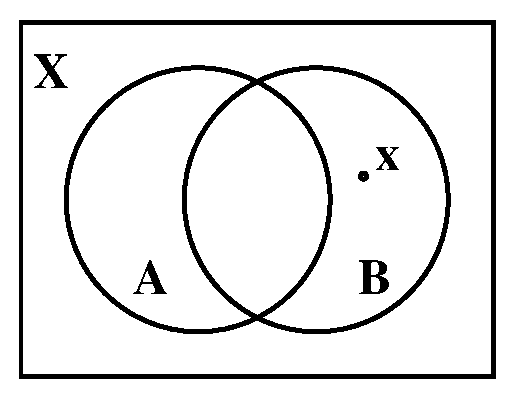
\includegraphics[width=6cm]{kuvat/venn}
\end{center}

Jos kaikki joukon $A$ alkiot ovat myös joukon $B$ alkioita, niin joukkoa $A$ kutsutaan joukon $B$ {\em osajoukoksi}. Osajoukkoa merkitään $A\subset B$. 

%{\bf KUVA}

\begin{center}
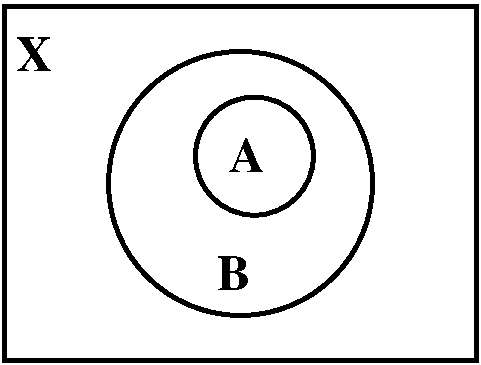
\includegraphics[width=6cm]{kuvat/osajoukko}
\end{center}

Jos $A\subset B$ ja $B\subset A$, niin  $A$ ja $B$ ovat sama joukko. Tällöin merkitään $A=B$. Samuus tarkoittaa sitä, että kyseisillä joukoilla on samat alkiot. % {\bf (toistoa, mitä pitäisikö siirtää aikaisemmaksi)}

{\bf Esimerkki 1.}
Akaan kaupunki muodostuu Toijalan, Viialan ja Kylmäkosken
kylistä. Akaa taas on osa Pirkanmaan maakuntaa. Olkoot $A
= \{\textrm{akaalaiset}\}$, $T = \{\textrm{toijalalaiset}\}$, $V
= \{\textrm{viialalaiset}\}$, $K = \{\textrm{kylmäkoskelaiset}\} $ ja $P = \{\textrm{pirkanmaalaiset}\}$. Onko lause tosi?

\begin{itemize}
\item[a)] $V \subset A$
\item[b)] $A \subset T$
\item[c)] $A \subset P$
\item[d)] $K \subset P$
\end{itemize}

(Sopiva kuva/kartta?)

{\bf Ratkaisu.}
a) Kaikki viialalaiset ovat akaalaisia, joten lause on
tosi.

b) Lauseen mukaan kaikki akaalaiset ovat toijalalaisia.
Lause on epätosi.

c) Kaikki akaalaiset ovat pirkanmaalaisia, joten lause on
tosi.

d) Lauseen mukaan kaikki kylmäkoskelaiset ovat
pirkanmaalaisia. Koska kylmäkoskelaiset ovat akaalaisia
ja akaalaiset pirkanmaalaisia, niin lause on tosi.

{\bf Vastaus:} a) On. b) Ei ole. c) On. d) On.

Ne perusjoukon $X$ alkiot, jotka eivät kuulu joukkoon $A$, muodostavat joukon $A$ {\em komplementin}. Joukon $A$ komplementtia merkitään $\complement A$.

\begin{center}
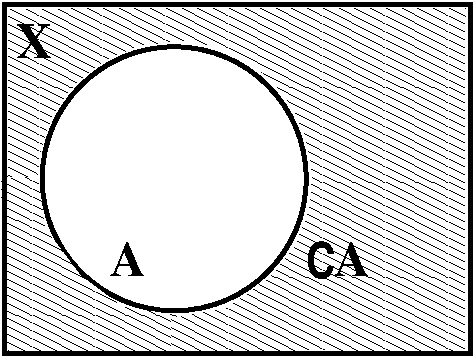
\includegraphics[width=6cm]{kuvat/komplementti}
\end{center}

Perusjoukon $X$ komplementti on {\em tyhjä joukko}, jota merkitään $\emptyset$. Tyhjässä joukossa ei ole alkioita. Erityisesti tyhjä joukko on minkä tahansa joukon osajoukko.

%{\bf KUVA}

Joukkojen $A$ ja $B$ {\em leikkaus} $A\cap B$ on niiden perusjoukon alkioiden joukko, jotka kuuluvat sekä joukkoon $A$ että joukkoon $B$. Leikkausta voidaan havainnollistaa Venn-diagrammilla:

\begin{center}
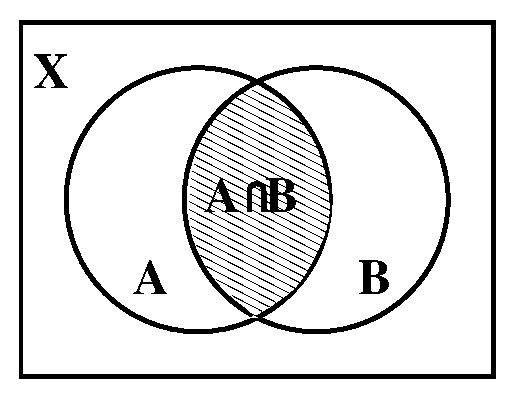
\includegraphics[width=6cm]{kuvat/leikkaus}
\end{center}

%{\bf KUVA}

Joukkojen $A$ ja $B$ {\em yhdiste} $A\cup B$ muodostuu niistä perusjoukon alkioista, jotka kuuluvat jompaankumpaan joukoista $A$ ja $B$. 
Joukkojen yhdistettä voidaan jälleen havainnollistaa Venn-diagrammin avulla:

\begin{center}
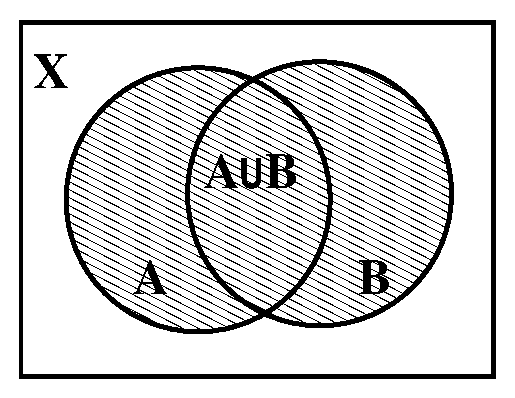
\includegraphics[width=6cm]{kuvat/yhdiste}
\end{center}

%{\bf KUVA}

%(Venn-diagrammit, matemaattisen väitteen totuus, avoin lause)

Joukkojen $A$ ja $B$ {\em erotuksella} tarkoitetaan joukkoa, joka jää jäljelle, kun joukosta $A$ poistetaan kaikki joukon $B$ alkiot. Tätä joukkoa merkitään $A\setminus B$. 

\begin{center}
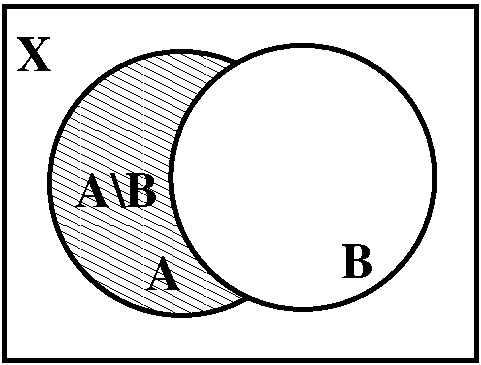
\includegraphics[width=6cm]{kuvat/erotus}
\end{center}


{\bf Esimerkki 2.}
Olkoot $A = \{0, 1, 2, 3, 4, 5, 6\}$ ja $B = \{2, 4, 6, 8, 10\}$. Määritä joukot a) $A\cup B$ b) $A \cap B$ c) $A\setminus B$ d) $B \setminus A$.

{\bf Ratkaisu:} 
a) Joukkojen $A$ ja $B$ yhdisteeseen $A \cup B$ kuuluvat ne alkiot, jotka kuuluvat jompaankumpaan joukoista $A$ ja $B$. Siten $A\cup B = \{0, 1, 2, 3, 4, 5, 6, 8, 10\}$.

b) Joukkojen $A$ ja $B$ leikkaukseen $A \cap B$ kuuluvat ne alkiot, jotka kuuluvat sekä joukkoon $A$ että joukkoon $B$. Siten $A \cap B = \{2, 4, 6\}$.

c) Joukkojen $A$ ja $B$ erotukseen $A \setminus B$ kuuluvat ne alkiot, jotka kuuluvat joukkoon $A$, mutta eivät joukkoon $B$. Siten $A \setminus B = \{0, 1, 3, 5\}$.

d) Vastaavasti erotukseen $B \setminus A$ kuuluvat ne alkiot, jotka kuuluvat joukkoon $B$, mutta eivät joukkoon $A$. Siten $B \setminus A = \{8, 10\}$.

{\bf Vastaus:} a) $A \cup B = \{0, 1, 2, 3, 4, 5, 6, 8, 10\}$,  b) $A \cap B = \{2, 4, 6\}$,  c) $A \setminus B = \{0, 1, 3,5\}$,  d) $B \setminus A = \{8, 10\}$.



{\bf Esimerkki 3.}
Koulussa on $700$ opiskelijaa. Erään kyselyn tuloksena saatiin selville, että $550$ heistä 
seuraa uutisia säännöllisesti sanomalehdistä ja $400$ Internetistä. Opiskelijoista $350$  
seuraa uutisia säännöllisesti kummastakin lähteestä. Havainnollista tilannetta Venn-diagrammilla ja vastaa seuraaviin kysymyksiin.
\begin{itemize}
\item[a)] Kuinka moni opiskelija seuraa uutisia vain Internetistä?
\item[b)] Kuinka moni opiskelija ei seuraa uutisia ollenkaan?
\end{itemize}

{\bf Ratkaisu:}

%[Venn-diagrammi]		
\begin{center}
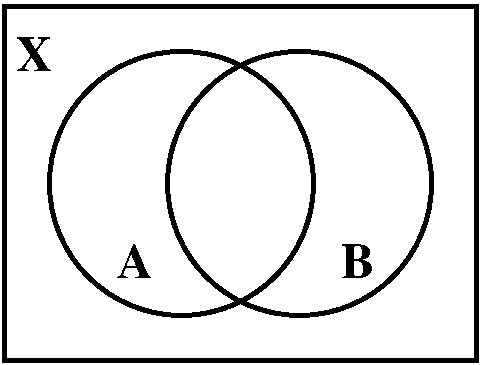
\includegraphics[width=6cm]{kuvat/venn2}
\end{center}

Perusjoukko $X$ sisältää kaikki koulun opiskelijat. Joukkoon $A$ kuuluvat opiskelijat, jotka seuraavat uutisia sanomalehdistä, ja joukkoon $B$ opiskelijat, jotka seuraavat uutisia Internetistä.

a) Opiskelijoista $400$ seuraa uutisia Internetistä ja $350$ heistä seuraa uutisia myös sanomalehdistä. Näin ollen $400 - 350 = 50$ opiskelijaa seuraa uutisia vain Internetistä. Tämä on joukon $B \setminus A$ alkioiden lukumäärää. 

b) Ainakin toisesta lähteestä uutisia seuraa $550 + 400 - 350 = 600$ opiskelijaa. Tällöin $700 - 600 = 100$ opiskelijaa ei seuraa uutisia ollenkaan. Tämä on joukon $\compl(A\cup B)$ alkioiden lukumäärä.

{\bf Vastaus:} a) $50$ opiskelijaa b) $100$ opiskelijaa


{\bf Esimerkki 4.} Olkoot perusjoukko $\R$ sekä joukot $A$ ja $B$ reaalilukuvälit $A = ]-5, 1]$ ja $B = ]-2, 4]$. Ilmaise välimerkintää käyttäen joukot a) $A\cup B$, b) $A \setminus B$, c) $\compl A$, d) $\compl( A \cap B)$. {\bf (lukusuora jonnekin?)}  

{\bf Ratkaisu:} 
\begin{itemize}
\item[a)] Joukkojen $A$ ja $B$ yhdisteeseen $A \cup B$ kuuluvat ne luvut, jotka kuuluvat jompaankumpaan joukoista $A$ ja $B$. Siten $A\cup B = ]-5, 4]$.
\item[b)] Joukkojen $A$ ja $B$ erotukseen $A \setminus B$ kuuluvat ne luvut, jotka kuuluvat joukkoon $A$, mutta eivät joukkoon $B$. Siten $A \setminus B = ]-5, -2]$.
\item[c)] Joukon $A$ komplementtiin $\compl A$ kuuluvat ne reaaliluvut, jotka eivät kuulu joukkoon $A$. Komplementti muodostuu väleistä $]-\infty, -5]$ ja $]1, \infty [$. Siten $\compl A = ]-\infty, -5] \cup ]1, \infty [$.
\item[d)] Joukkojen $A$ ja $B$ leikkaukseen kuuluvat ne luvut, joka kuuluvat sekä joukkoon $A$ että joukkoon $B$. Siten $A\cap B = ]-2, 1]$. Leikkauksen komplementtiin kuuluvat kaikki muut reaaliluvut, joten $\compl( A \cap B) = ]-\infty, -2] \cup ]1,\infty [$.
\end{itemize}

{\bf Vastaus:}
\begin{itemize}
\item[a)] $A\cup B =]-5, 4]$,
\item[b)] $A \setminus B = ]-5, -2]$,
\item[c)] $\compl A = ]-\infty, -5] \cup ]1, \infty [$,
\item[d)] $\compl( A \cap B) = ]-\infty, -2] \cup ]1,\infty [$.
\end{itemize}


{\bf Esimerkki 5.} Osoita Venn-diagrammia käyttäen, että $\compl A \cap B = B \setminus A$.

{\bf Ratkaisu:}

%[Venn-diagrammi, jossa on esitetty $\compl A \cap B$]

\begin{center}
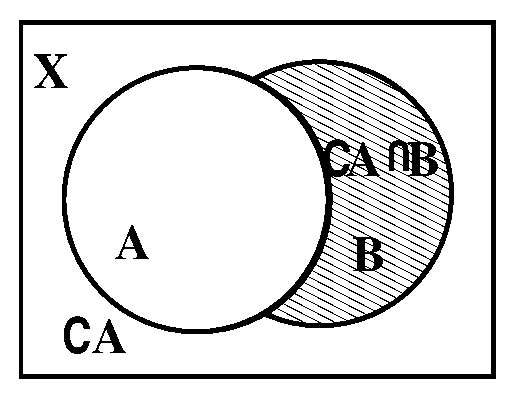
\includegraphics[width=6cm]{kuvat/esim4-3_2b}
\end{center}

Joukon $A$ komplementtijoukko $\compl A$ on niiden perusjoukon alkioiden joukko, jotka eivät kuulu joukkoon $A$, ja $\compl A\cap B$ on tämän joukon leikkaus joukon $B$ kanssa.

%[Venn-diagrammi, jossa on esitetty $B \setminus A$]

\begin{center}
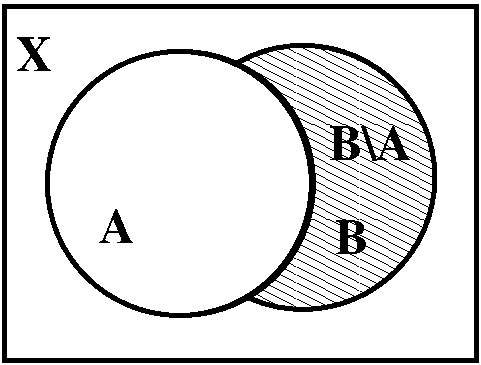
\includegraphics[width=6cm]{kuvat/esim4-3_2}
\end{center}

Joukko $B \setminus A$ sisältää ne joukon $B$ alkiot, jotka eivät kuulu joukkoon $A$.
Venn-diagrammit havainnollistavat, että on kyse samasta joukosta. Siis $\compl A\cap B = B \setminus A$.


\newpage


\subsection*{Tehtäviä}

\begin{enumerate}

\item Onko lause tosi?
\begin{itemize}
\item[a)] $K \subset A$
\item[b)] $A \subset V$
\item[c)] $V \subset P$
\item[d)] $V \subset T$
\end{itemize}
Merkinnät ovat samat kuin esimerkissä 1.

\item Olkoot $A = \{7,8,9\}$ ja $B=\{5,6,7\}$. Määritä joukot
\begin{itemize}
\item[a)] $A \cup B$,
\item[b)] $A \cap B$,
\item[c)] $A \setminus B$,
\item[d)] $B \setminus A$.
\end{itemize}

\item Olkoot perusjoukko $X$ aakkoset, $A$ vokaalit ja $B=\{x,y,z\}$.
Määritä joukot
\begin{itemize}
\item[a)] $B\setminus A$,
\item[b)] $A\cap B$,
\item[c)] $\complement A$,
\item[d)] $A \setminus X$.
\end{itemize}


\item
Olkoot $A$ koulussa opiskelevien täysi-ikäisten opiskelijoiden joukko ja $B$ niiden opiskelijoiden joukko, jotka asuvat vanhempiensa luona. Millaiset opiskelijat kuuluvat joukkoon a) $A \cap B$,  b) $\compl A$, c) $A \cup \compl B$, d) $A\setminus B$, e) $B \setminus A$, f) $\compl (A \cup B)$?

\item
Ilmaise joukkomerkintöjä käyttäen kuvan
\begin{itemize}
\item[a)] keltainen alue,
\item[b)] sininen alue,
\item[c)] violetti alue,
\item[d)] vihreä alue.
\end{itemize}

\begin{center}
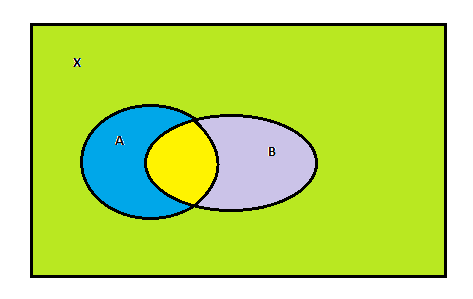
\includegraphics[width=10cm]{kuvat/mika2}
\end{center}
%PICXX2

\item
Olkoot $A \cap B$, $A \setminus B$ ja $B \setminus A$ epätyhjiä joukkoja. Esitä Venn-diagrammissa varjostettuna alue, joka kuvaa joukkoa a) $\compl (A \cup B)$, b) $\compl (A \cap B)$, c) $\compl B \cap A$.

\item Luokalla on 30 opiskelijaa. Heistä 14 harrastaa jääkiekkoa, 12 jalkapalloa ja 3 molempia. 
\begin{itemize}
\item[a)] Kuinka moni opiskelija harrastaa pelkkää jääkiekkoa?
\item[b)] Kuinka moni opiskelija harrastaa pelkkää jalkapalloa?
\item[c)] Kuinka moni opiskelija ei harrasta kumpaakaan?
\end{itemize}
Vihje: Tilanteesta kannattaa piirtää Venn-diagrammi.

\item Olkoot perusjoukko $\R$ sekä joukot $A$ ja $B$ reaalilukuvälit $A=[1,5]$ ja $B=[3,6]$. Ilmaise välimerkintää käyttäen joukot
\begin{itemize}
\item[a)] $A \cap B$,
\item[b)] $A \cup B$,
\item[c)] $A \setminus B$,
\item[d)] $\compl A$.
\end{itemize}

\item Yhdistä samaa tarkoittavat lauseet.
\[
\begin{array}{llll}
A & (x\in A)\land (x\in B) & 1 & x\in \complement A \\
B & x\notin A & 2 & x \in A\setminus B \\
C & (x\in A)\lor (x\in B) & 3 & x\in (A\cap B) \\
D & (x\in A)\land (x\notin B) & 4 & x\in (A\cup B)
\end{array}
\]

\item Osoita Venn-diagrammin avulla, että
\begin{itemize}
\item[a)] 
\[
A\cup (B \cap C) = (A\cup B)\cap(A\cup C),
\]
\item[b)] 
\[
A\cap (B \cup C) = (A\cap B)\cup(A\cap C).
\]
\end{itemize}

\item Sievennä Venn-diagrammin avulla.
\begin{itemize}
\item[a)] $(B\cap A) \cup (B \cap \compl A)$
\item[b)] $\compl (A\cup B) \cup (A \setminus B) \cup (B \setminus A)$
\end{itemize}

\item
Olkoot perusjoukko kokonaislukujen joukko $\mathbb{Z}$, $W$ parillisten kokonaislukujen joukko ja $Y$ luvulla $3$ jaollisten kokonaislukujen joukko. Näitä joukkoja voidaan merkitä $W = \{2n\,|\, n\in\Z\}$ ja $Y = \{3n \,|\, n \in \Z\}$. Määritä joukot a) $W \cap Y$, b) $W \setminus Y$, c) $W \cup Y$.

\item Onko lause tosi?
\begin{itemize}
\item[a)] $\sqrt{2} \in \R$
\item[b)] $-3 \in \N$
%\item[c)] $\Z \subset \Q$
\item[c)] $\pi \in \R \setminus \Q$
\item[d)] $\frac{4}{2} \in \Q \setminus \Z$
\item[e)] $\emptyset \subset \Z$
\end{itemize}

\item Määritä joukon a) $\{1,2\}$ b) $\{1,2,3\}$ kaikki osajoukot.

\item (Lisämateriaalia) Joukon $A$ {\em potenssijoukoksi} $\mathcal{P}(A)$ kutsutaan kaikkien joukon $A$ osajoukkojen muodostamaa joukkoa:
\[
\mathcal{P}(A)=\{ B \, | \, B\subset A\}.
\]
\begin{itemize}
\item[a)] Määritä joukon $\{1,2,3\}$ potenssijoukko.
\item[b)] Määritä tyhjän joukon $\emptyset$ potenssijoukko.
\item[c)] Joukko $\{\emptyset\}$ on joukko, jonka ainut alkio on tyhjä joukko. Määritä joukon $\{\emptyset\}$ potenssijoukko.
\end{itemize}

\item (Lisämateriaalia) Luonnolliset luvut voidaan tulkita joukko-opillisesti käyttämällä edellisessä tehtävässä esitettyä potenssijoukon käsitettä. Ajatuksena on, että lukua $0$ vastaa tyhjä joukko $\emptyset$ ja kutakin luonnollista lukua $n + 1$ vastaava joukko on luonnollista lukua $n$ vastaavan joukon potenssijoukko. Siis esimerkiksi lukua $1$ vastaa tyhjän joukon $\emptyset$ potenssijoukko $\mathcal{P}(\emptyset)$, lukua $2$ potenssijoukko $\mathcal{P}(\mathcal{P}(\emptyset))$ ja niin edelleen.
\begin{itemize}
\item[a)] Määritä lukuja $3$ ja $4$ vastaavat joukot.
\item[b)] Mitä luonnollista lukua vastaa joukko $\{\emptyset,\{\emptyset\}\}$?
\item[c)] Vastaako joukko $\{\{\emptyset\}\}$ jotakin luonnollista lukua? Miksi?
\end{itemize}

\end{enumerate}

{\bf Kotitehtäviä}

\begin{enumerate}

\item Olkoot $A = \{a,b,c,d\}$ ja $B=\{a,c,e\}$. Määritä joukot
\begin{itemize}
\item[a)] $A \cup B$, 
\item[b)] $A \cap B$,
\item[c)] $A \setminus B$,
\item[d)] $B \setminus A$.
\end{itemize}

\item Onko lukujoukkoja koskeva lause tosi?
\begin{itemize}
\item[a)] $\Z \subset \N$
\item[b)] $\Z \subset \Q$
\item[c)] $\R \subset \Z$
\item[d)] $\Q \subset \N$
\item[e)] $\Q \subset \Q$
\end{itemize}

\item Olkoot perusjoukko $X$ aakkoset, $A=\{j,o,k,u\}$, $B=\{k,o,j,u\}$ ja $C=\{k,a,j,o\}$. Määritä joukot
\begin{itemize}
\item[a)] $A\setminus B$,
\item[b)] $(A\cap B)\cup C$,
\item[c)] $A\setminus \complement (B\cup C)$.
\end{itemize}

\item Olkoot $X$ perusjoukko ja $A$ jokin perusjoukon osajoukko. Sievennä.
\begin{itemize}
\item[a)] $A\cup \emptyset$
\item[b)] $A\cap \emptyset$
\item[c)] $A\cap X$
\item[d)] $A\cup X$
\end{itemize}

\item
Olkoot $A \subset B$ ja $B \setminus A$ epätyhjä. Esitä Venn-diagrammissa varjostettuna alue, joka kuvaa joukkoa a) $B \setminus A$, b) $\compl A \cap B$, c) $A \cup \compl B$.

\item
Olkoon perusjoukko $X$ kaikkien kalenterivuoden päivien joukko. Olkoot $A$ arkipäivien (maanantai--perjantai) joukko, $L$ liputuspäivien joukko ja $T$ toukokuulle ajoittuvien päivien joukko. Millaiset päivät kuuluvat joukkoon
\begin{itemize}
\item[a)] $\compl A$
\item[b)] $L \cap \compl T$
\item[c)] $L \setminus A$
\item[d)] $T \setminus (A \cup L)$
\item[e)] $\compl (A \cup L \cup T)$?
\end{itemize}

\item Onko lause tosi?
\begin{itemize}
\item[a)] $0 \in \{0,1,2\}$
\item[b)] $\{0\} \subset \{0,1,2\}$
\item[c)] $\emptyset \subset \{1,2\}$
\item[d)] $\{\textrm{å},\textrm{ä},\textrm{ö}\} \subset \{\textrm{o},\textrm{ä},\textrm{ö}\}$
\end{itemize}

\item Luokan opiskelijoista kahdeksalla on läppäri, kymmenellä pöytäkone ja
viidellä tabletti.
Kahdella opiskelijalla on sekä läppäri että pöytäkone, kolmella sekä
tabletti että pöytäkone, mutta kellään ei ole sekä läppäriä että
tablettia. Kahdella opiskelijalla ei ole mitään tietokonetta.
\begin{itemize}
\item[a)] Piirrä tilannetta kuvaava Venn-diagrammi.
\item[b)] Kuinka monella opiskelijalla on läppäri mutta ei pöytäkonetta?
\item[c)] Kuinka monella opiskelijalla on vain pöytäkone?
\item[d)] Kuinka monta opiskelijaa luokalla on?
\end{itemize}

\item Olkoot perusjoukko $\R$ sekä joukot $A$ ja $B$ reaalilukuvälit $A=]-1,2[$ ja $B=[0,4[$. Ilmaise välimerkintää käyttäen joukot
\begin{itemize}
\item[a)] $A \cup B$,
\item[b)] $A \cap B$,
\item[c)] $\compl (A \cap B)$,
\item[d)] $B \setminus A$,
\item[e)] $B \setminus (A \cap B)$,
\item[f)] $A \cap \compl B$.
\end{itemize}

\item Osoita Venn-diagrammin avulla, että
\begin{itemize}
\item[a)] 
\[
X\setminus (A\cup B) = (X\setminus A)\cap (X\setminus B),
\]
\item[b)] 
\[
X \setminus (A\cap B) = (X\setminus A)\cup (X\setminus B).
\]
\end{itemize}

\item Jos $A\subset B$ ja $B\subset C$, niin mitä voidaan päätellä joukoista $A$ ja $C$? Perustele 
\begin{itemize}
\item[a)] Venn-diagrammin avulla,
\item[b)] osajoukon määritelmän avulla.
\end{itemize}

\item
Onko lause tosi?
\begin{itemize}
\item[a)] $A \cap B \subset A$
\item[b)] $\compl (\compl A) = A$
\item[c)] $(A\cup B) \setminus B = A$
\item[d)] $A \cap \compl B = A \setminus B$
\item[e)] $B \cap \compl B = B$
\end{itemize}

\item Ilmaise joukkomerkintöjä käyttäen kuvan
\begin{itemize}
\item[a)] punainen alue,
\item[b)] sininen alue,
\item[c)] vihreä alue,
\item[d)] keltainen alue.
\end{itemize}

\begin{center}
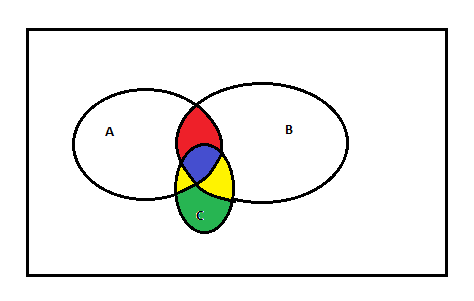
\includegraphics[width=10cm]{kuvat/mika3}
\end{center}
%PICXX3

\item Tarkastellaan kaksinumeroisia luonnollisia lukuja $10,11, \ldots ,98,99$.
\begin{itemize}
\item[a)] Kuinka monta kaksinumeroista luonnollista lukua on olemassa?
\item[b)] Kuinka moni niistä on jaollinen luvulla $4$? Kuinka moni ei ole jaollinen luvulla $4$?
\item[c)] Kuinka moni kaksinumeroisista luonnollisista luvuista on jaollinen luvulla $6$?
\item[d)] Kuinka moni kaksinumeroisista luonnollisista luvuista on jaollinen luvuilla $4$ ja $6$?
\item[e)] Kuinka moni kaksinumeroisista luonnollisista luvuista on jaollinen luvulla $4$ tai luvulla $6$?
\item[f)] Kuinka moni kaksinumeroisista luonnollisista luvuista ei ole jaollinen luvulla $4$ eikä luvulla $6$?
\item[g)] Piirrä tilanteesta Venn-diagrammi.
\end{itemize}

\end{enumerate}

\newpage


\subsection{Avoin lause ja konnektiivien joukko-opillinen tulkinta.}

\subsection*{Tutkimustehtävä}
\begin{itemize}
\item[1)] Ketkä seuraavista henkilöistä toteuttavat väitteen ''henkilö on entinen Suomen tasavallan presidentti''? 
a) Urho Kekkonen,  b)  Paavo Nurmi,  c)  Armi Kuusela,  d)  Tarja Halonen,  
e) Carl Gustaf Emil Mannerheim.
\item[2)] 
Lause $P(x)$ on ''$-10x = 100$''. Onko lause $P(-2)$, $P(5)$ tai $P(-10)$ tosi?
\item[3)] 
Millä kokonaisluvuilla lause $Q(x)$: ''$2x^2 - x - 1 = 0$'' on tosi?
\end{itemize}

{\bf Avoin lause ja ratkaisujoukko.}
Lauselogiikassa asioiden tiloja ilmaisemaan käytetään atomilauseita, esimerkiksi lausetta $S$: ''sataa''. Tämän lauseen totuusarvo kuitenkin riippuu tarkastelijan olinpaikasta $x$. Onkin luonnollinen ajatus tarkastella loogista lausetta, jossa on {\em vapaa muuttuja}, tässä tapauksessa paikka $x$. Tällöin merkitään $S(x)$: ''paikassa $x$ sataa''. Lauseen totuusarvo ratkeaa vasta, kun vapaan muuttujan arvo kiinnitetään. Siksi lausetta $S(x)$ kutsutaan {\em avoimeksi lauseeksi}. Avoimia lauseita kutsutaan myös {\em predikaateiksi}, ja avoimia lauseita käsittelevää logiikkaa sanotaan {\em predikaattilogiikaksi}.

Vapaa muuttuja saa arvoja annetusta perusjoukosta $X$. Perusjoukkoa ei ole tapana kirjoittaa näkyviin, jos se voidaan päätellä tilanteesta. Esimerkiksi yllä mainitussa avoimessa lauseessa $S(x)$ perusjoukkona ovat kaikki paikkakunnat. Avoimen lauseen {\em ratkaisujoukon} muodostavat puolestaan ne perusjoukon alkiot, joilla avoin lause on tosi. Esimerkiksi lauseen $S(x)$ ratkaisujoukkona ovat kaikki ne paikkakunnat, joilla sataa.

Avoimessa lauseessa voi olla useampiakin muuttujia, voitaisiin esimerkiksi tarkastella lausetta $S(x,t)$: ''paikassa $x$ sataa hetkellä $t$''. Monimutkaisempia avoimia lauseita voidaan muodostaa konnektiivien
avulla.

Matematiikassa avoin lause on usein yhtälö tai epäyhtälö. Yhtälössä esiintyvät tuntemattomat voidaan tulkita vapaiksi muuttujiksi. Esimerkiksi voidaan merkitä $C(x)$: ''$\cos x + x^2= 2$''. Avoimen lauseen ratkaisujoukko on niiden pisteiden $x$ joukko, joilla kyseinen yhtälö toteutuu.


{\bf Esimerkki 1.} Olkoon $P(x)$ avoin lause ''$2x - 10 = 0$''. Onko lause a) $P(5)$, b) $P(-5)$ tosi?

{\bf Ratkaisut:}

a) Sijoitetaan luku $5$ avoimeen lauseeseen muuttujan $x$ paikalle. Koska $2\cdot 5 - 10 = 10 - 10 = 0$, lause $P(5)$ on tosi.

b) Sijoitetaan luku $-5$ avoimeen lauseeseen muuttujan $x$ paikalle. Koska $2\cdot(-5) - 10 = -10 - 10 = -20 \neq 0$, lause $P(-5)$ on epätosi.

{\bf Vastaukset:} a) On. b) Ei ole.

{\bf Esimerkki 2.} Yhtälöiden ja epäyhtälöiden yhteydessä perusjoukkoa kutsutaan myös {\em määrittelyjoukoksi}. Ratkaise avoin lause $2x^2 + 5x - 3 < 0$, kun määrittelyjoukko on a) reaalilukujen joukko b) kokonaislukujen joukko.

{\bf Ratkaisut:}

a) Tutkitaan polynomifunktion $2x^2 + 5x - 3$ merkkiä. Ratkaistaan funktion $2x^2 + 5x - 3$ nollakohdat toisen asteen yhtälön ratkaisukaavalla.
\[
2x^2 + 5x - 3 = 0
\]
\[
x =\frac{-5\pm\sqrt{5^2-4\cdot 2\cdot(-3)}}{2\cdot 2}
\] 
\[
x = \frac{-5\pm\sqrt{49}}{4} =\frac{-5\pm 7}{4}
\]
\[
x = -3\textrm{  tai  }x =\frac{1}{2}.
\]
Koska funktion $2x^2 + 5x - 3$ kuvaaja on ylöspäin aukeava paraabeli, avoin lause $2x^2 + 5x - 3 < 0$ toteutuu, kun $-3 < x < \frac{1}{2}$. Avoimen lauseen ratkaisujoukko on siis väli $]-3, \frac{1}{2}[$.

b) Kun määrittelyjoukko on kokonaislukujen joukko, a-kohdan ratkaisuista kelpaavat vain $x = -2$, $x = -1$ ja $x = 0$. Avoimen lauseen ratkaisujoukko on siis $\{-2, -1, 0\}$.

{\bf Vastaukset:} a) $-3 < x < \frac{1}{2}$, b) $x = -2$ tai $x = -1$ tai $x = 0$

{\bf Ominaisuudet ja osajoukot.}
Jouk\-ko-opin soveltamisen kannalta on usein hyödyllistä {\em samastaa} keskenään joukot ja perusjoukon $X$ alkioiden ominaisuudet. Tällöin avoimelle lauseelle $P(x)$ käytetään myös merkintää $x\in P$. Jos $\lnot P(y)$, voidaan merkitä $y\notin P$. Tätä voidaan havainnollistaa Venn-diagrammilla. Kuvassa $x\in P$ ja $y\notin P$.

%{\bf kuva}.
\begin{center}
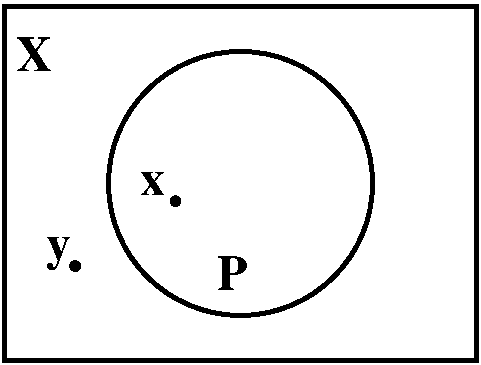
\includegraphics[width=6cm]{kuvat/kuuluu}
\end{center}

Jos predikaatit ajatellaan perusjoukon osajoukoiksi, niin joukko-opil\-li\-set operaatiot voidaan tulkita loogisina operaatioina. Kahden predikaatin $P$ ja $Q$ konjunktiota $P\land Q$ vastaa joukko-opissa leikkaus $P\cap Q$, disjunktiota $P \lor Q$ yhdiste $P\cup Q$ ja negaatiota $\lnot P$ komplementtijoukko $\complement P$. 
Tarkastellaan implikaation $P(x)\to Q(x)$ totuustaulua:

\bigskip

\begin{center}
\begin{tabular}{|c|c|c|}\hline
$x\in P$ & $x \in Q$ & $P(x) \to Q(x)$ \\ \hline
$1$ & $1$ & $1$\\ %\hline
$1$ & $0$ & $0$\\
$0$ & $1$ & $1$\\
$0$ & $0$ & $1$\\ \hline
\end{tabular}
\end{center}

\bigskip

Nähdään, että implikaatio on epätosi vain silloin, jos $x \in P$ mutta $x\not \in Q$, toisin sanoen $P$ ei ole $Q$:n osajoukko. Implikaatiota $P \to Q$ vastaa siis sisältymisrelaatio $P \subset Q$. Erityisesti periaatetta, että epätodesta lauseesta voidaan päätellä mitä tahansa, vastaa se, että tyhjä joukko $\emptyset$ on minkä tahansa joukon osajoukko. Ekvivalenssia $P\lequiv Q$ vastaava relaatio on joukko-opillinen yhtäsuuruus $P=Q$.


{\bf Esimerkki 3.} Olkoon perusjoukko kuviossa olevien nelikulmioiden joukko. Olkoot avoin lause $K(x)$: ''nelikulmio $x$ on suorakulmio'' ja $S(x)$: ''nelikulmio $x$ on suunnikas''. Ratkaise avoin lause.  a)  $K(x)$,  b)  $S(x)$,  c) $\lnot S(x)$,  d)  $\lnot K(x) \land S(x)$  e)  $K(x) \lequiv S(x)$.

\begin{center}
%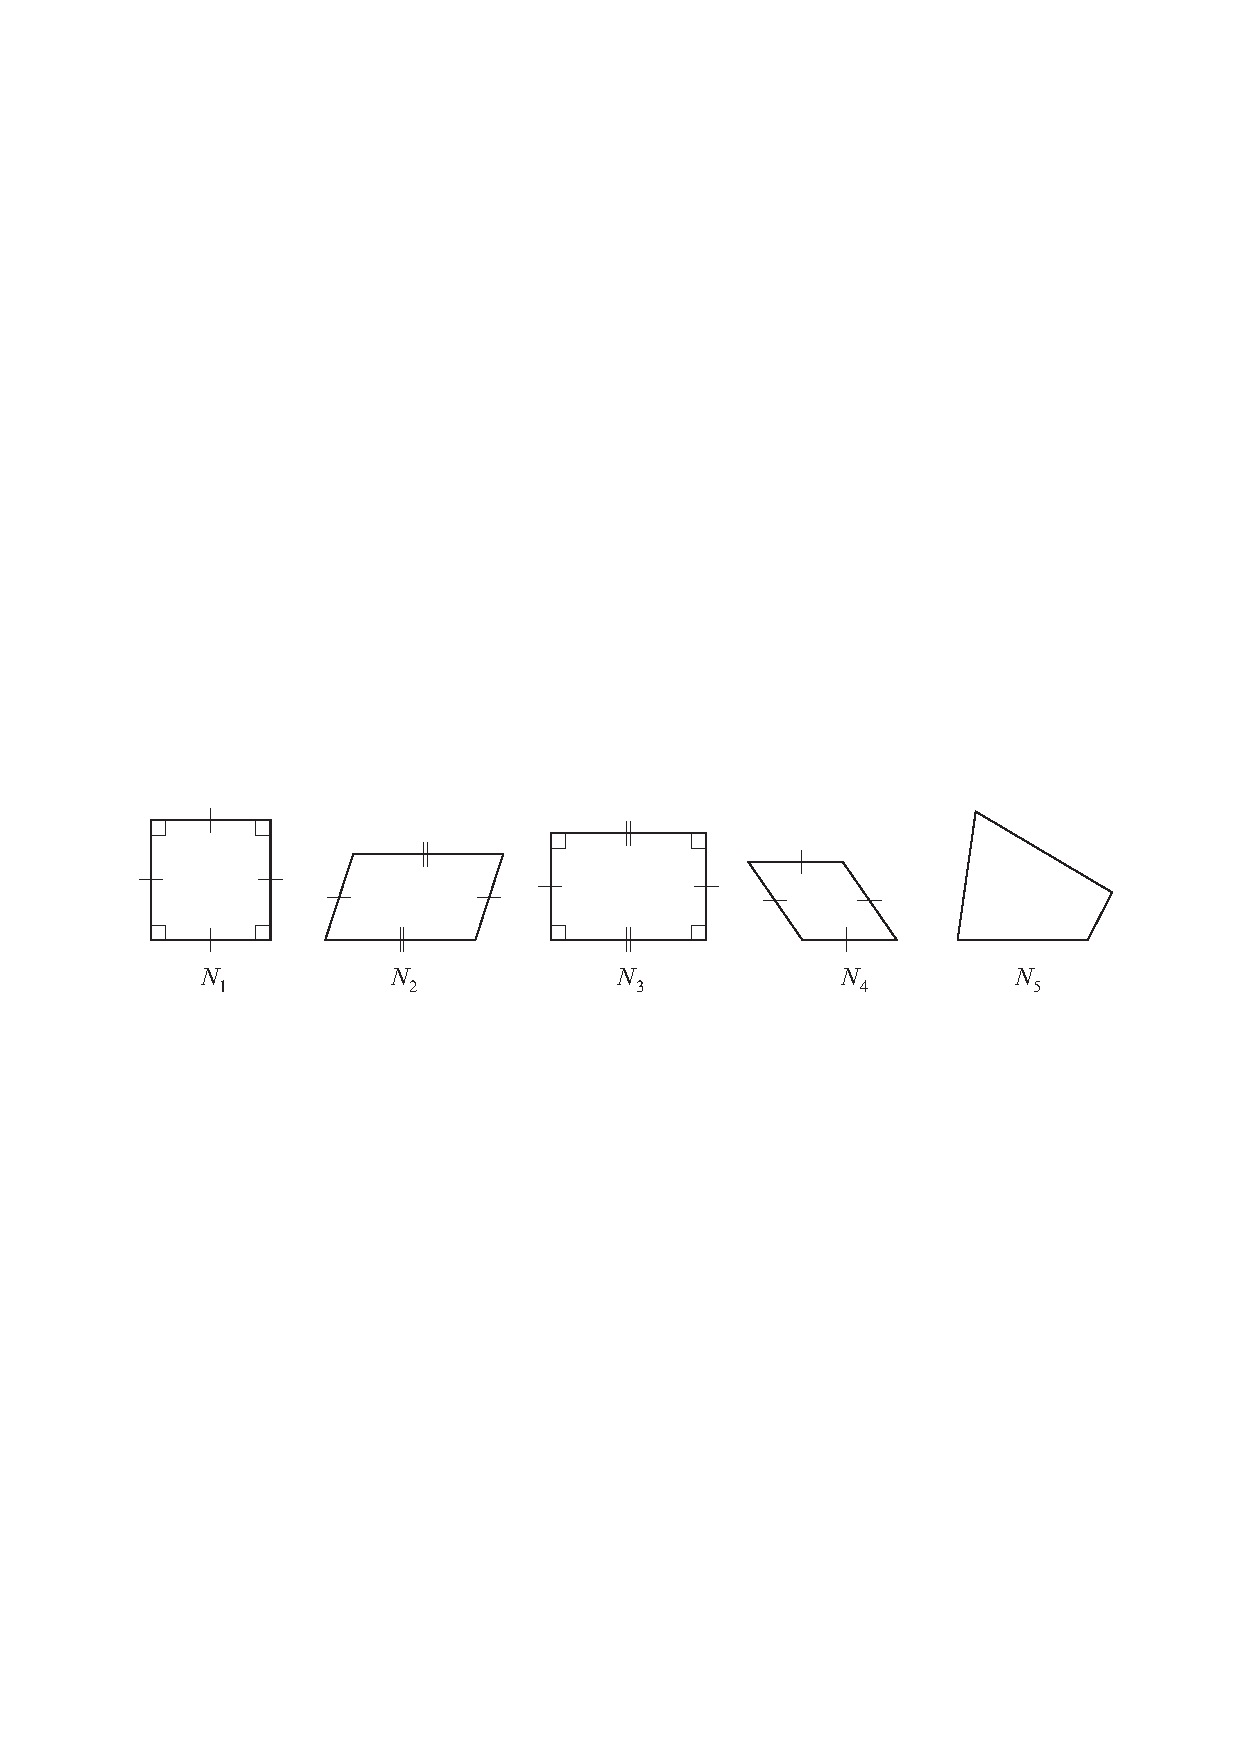
\includegraphics[width=12cm,height=4cm]{kuvat/Kappale3_2_esim_3_kuvio_v2}
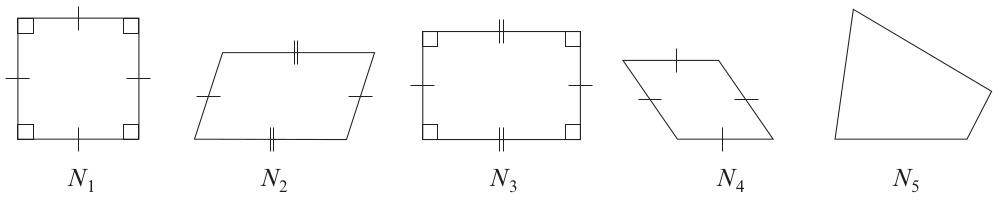
\includegraphics[width=14cm]{kuvat/kpl3_2_esim3}
\end{center}


{\bf Ratkaisut:}

a) Avoin lause $K(x)$ on tosi, kun nelikulmio on suorakulmio. Suorakulmioita ovat nelikulmiot $N_1$ ja $N_3$, joten ratkaisujoukko on $\{ N_1, N_3\}$.

b) Avoin lause $S(x)$ on tosi, kun nelikulmio on suunnikas. Suunnikkaita ovat nelikulmiot $N_1$, $N_2$, $N_3$ ja $N_4$, joten ratkaisujoukko on $\{ N_1, N_2, N_3, N_4\}$.

c) Negaatio $\lnot S(x)$ on tosi, kun avoin lause $S(x)$ on epätosi eli kun nelikulmio ei ole suunnikas. Ehto toteutuu vain nelikulmiolla $N_5$. Ratkaisujoukko on $\{N_5\}$.

d) Avoin lause $\lnot K(x) \land S(x)$ on tosi, kun nelikulmio on suunnikas mutta ei suorakulmio. Ehto toteutuu nelikulmioilla $N_2$ ja $N_4$, joten ratkaisujoukko on $\{ N_2, N_4\}$.

e) Avoin lause $K(x) \lequiv S(x)$ on tosi, kun nelikulmio on suorakulmio ja suunnikas tai ei kumpikaan. Ehto toteutuu nelikulmioilla $N_1$, $N_3$ ja $N_5$, joten ratkaisujoukko on $\{ N_1, N_3, N_5\}$.

{\bf Vastaukset:}   a)  $\{ N_1, N_3\}$,   b)  $\{ N_1, N_2, N_3, N_4\}$,   c)  $\{N_5\}$,  d)  $\{ N_2, N_4\}$,  e)  $\{ N_1, N_3, N_5\}$.


{\bf Esimerkki 4.} Heitetään kahta noppaa, punaista ja sinistä. Tuloksena saadaan lukupari $(x, y)$, missä $x$ on punaisen nopan silmäluku ja $y$ on sinisen nopan silmäluku. Perusjoukko $X$ sisältää lukuparit
\[
(1, 1), (1, 2), (1, 3), (1, 4), (1, 5), (1, 6), (2, 1), (2, 2),\ldots , (6, 5), (6, 6).
\]
Olkoot avoimet lauseet $S(x,y)$: ''$x + y > 9$'' ja $Y(x,y)$: ''$x = y$''. Määritä avoimen lauseen a) $S(x,y)$, b) $Y(x,y)$, c) $\lnot S(x,y) \land Y(x,y)$, d) $\lnot S(x,y) \to Y(x,y)$ ratkaisujoukko.

\begin{center}
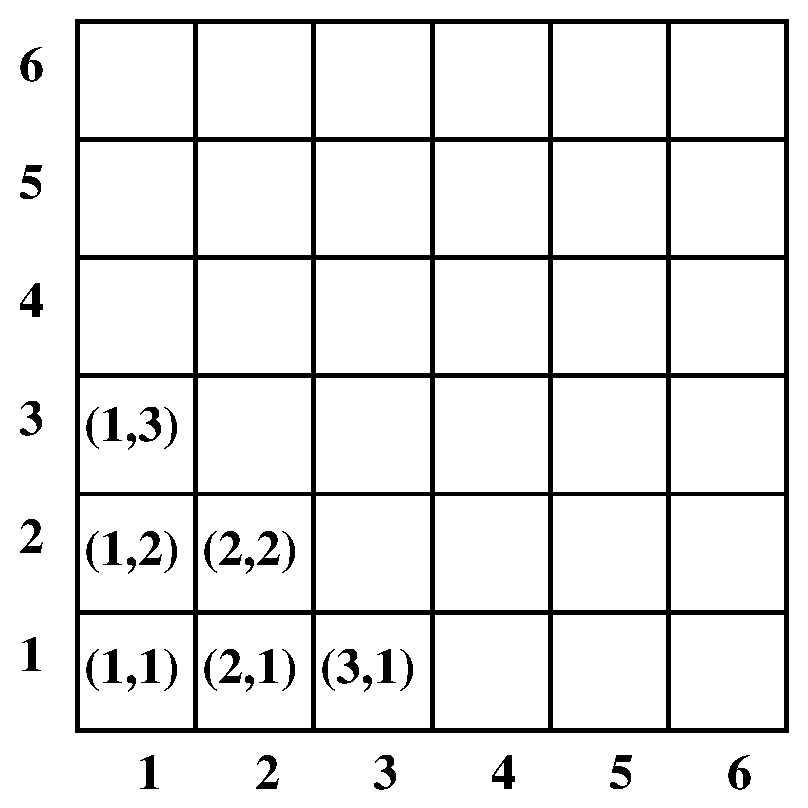
\includegraphics[width=6cm]{kuvat/6x6}
\end{center}

{\bf Ratkaisu:}

a) Avoin lause $S(x,y)$ on tosi, kun noppien silmälukujen summa on suurempi kuin $9$ eli siis $10, 11$ tai $12$. Ehto toteutuu lukupareilla $(4, 6), (5, 5), (5, 6), (6, 4), (6, 5)$ ja $(6, 6)$. Ratkaisujoukko on
\[
\{(4, 6), (5, 5), (5, 6), (6, 4), (6, 5), (6, 6)\}.
\]

b) Avoin lause $Y(x,y)$ on tosi, kun noppien silmäluvut ovat samat. Ehto toteutuu lukupareilla $(1, 1), (2, 2), (3, 3), (4, 4), (5, 5)$ ja $(6, 6)$. Ratkaisujoukko on $\{(1, 1), (2, 2), (3, 3), (4, 4), (5, 5), (6, 6)\}$.

c) Avoin lause $\lnot S(x,y) \land Y(x,y)$ on tosi, kun noppien silmälukujen summa on pienempi tai yhtä suuri kuin $9$ ja kun silmäluvut ovat samat. Ehto toteutuu lukupareilla $(1,1), (2, 2), (3, 3)$ ja $(4, 4)$. Ratkaisujoukko on $\{(1,1), (2, 2), (3, 3), (4, 4)\}$.


d) Implikaatio $\lnot S(x,y) \to Y(x,y)$ on tosi aina, kun avoin lause $\lnot S(x,y)$ on epätosi eli kun $S(x,y)$ on tosi. Avoimen lauseen $S(x,y)$ ratkaisujoukko on määritetty a-kohdassa. Lisäksi implikaatio $\lnot S(x,y) \to Y(x,y)$ on tosi silloin, kun avoimet lauseet $\lnot S(x,y)$ ja $Y(x,y)$ ovat molemmat tosia. Tämän tapauksen ratkaisujoukko on määritetty c-kohdassa. Implikaation $\lnot S(x,y) \to Y(x,y)$ ratkaisujoukko on siis
\[
\{(1,1), (2, 2), (3, 3), (4, 4), (4, 6), (5, 5), (5, 6), (6, 4), (6, 5), (6, 6)\}.
\]

{\bf Vastaukset:} a) $\{(4, 6), (5, 5), (5, 6), (6, 4), (6, 5), (6, 6)\}$

b) $\{(1, 1), (2, 2), (3, 3), (4, 4), (5, 5), (6, 6)\}$

c) $\{(1,1), (2, 2), (3, 3), (4, 4)\}$

d) $\{(1,1), (2, 2), (3, 3), (4, 4), (4, 6), (5, 5), (5, 6), (6, 4), (6, 5), (6, 6)\}$


{\bf Esimerkki 5.} Ratkaise reaalilukujen joukossa
\begin{itemize}
\item[a)] yhtälö $(x + 4)(x^2 - 2) = 0$,
\item[b)] yhtälöpari
\[
\left\{
\begin{array}{rcl}
x + 4 & = & 0, \\
x^2 - 2 & = & 0.
\end{array}\right.
\]
\end{itemize}

{\bf Ratkaisut:}

a) Tulon nollasäännön perusteella yhtälö $(x + 4)(x^2 -
2) = 0$ toteutuu, kun $x + 4 = 0$ tai $x^2 - 2 = 0$.

Yhtälö $x + 4 = 0$ toteutuu, kun $x = -4$.

Yhtälö $x^2 - 2 = 0$ eli $x^2 = 2$ toteutuu, kun $x =
\sqrt{2}$ tai $x = -\sqrt{2}$.

Siis yhtälö $(x + 4)(x^2 - 2) = 0$ toteutuu, kun $x =
-4$ tai $x = -\sqrt{2}$ tai $x = \sqrt{2}$. Yhtälön
ratkaisujoukko on $\{-4, -\sqrt{2}, \sqrt{2} \}$.

b) Yhtälöpari
\[
\left\{
\begin{array}{rcl}
x + 4 & = & 0, \\
x^2 - 2 & = & 0,
\end{array}\right.
\]
toteutuu niillä reaaliluvuilla, jotka toteuttavat
molemmat yhtälöt $x + 4 = 0$ ja $x^2 - 2 = 0$. a-kohdan
perusteella tiedetään, että ensimmäinen yhtälö toteutuu,
kun $x = -4$, ja jälkimmäinen, kun $x = -\sqrt{2}$ tai $x
= \sqrt{2}$. Koska yhtälöparin
\[
\left\{
\begin{array}{rcl}
x + 4 & = & 0, \\
x^2 - 2 & = & 0,
\end{array}\right.
\]
toteuttavat ne reaaliluvut, jotka toteuttavat sekä
lauseen ''$x = -4$'' että lauseen ''$x = -\sqrt{2}$ tai
$x = \sqrt{2}$'', nähdään, että yhtälöparilla ei ole
ratkaisuja. Yhtälöparin ratkaisujoukko on siis tyhjä
joukko $\emptyset$.

{\bf Vastaukset:}

a) $x = -4$ tai $x = -\sqrt{2}$ tai $x = \sqrt{2}$
b) Yhtälöparilla ei ole ratkaisuja.

\newpage


\subsection*{Tehtäviä}

\begin{enumerate}
\item
Olkoot $A(x)$ avoin lause ''paikkakunnalla $x$ paistaa
aurinko'' ja $T(x)$ avoin lause ''paikkakunnalla $x$
tuulee''. Suomenna lause.
\begin{itemize}
\item[a)] $\lnot T(x)$,
\item[b)] $A(x) \land T(y)$,
\item[c)] $\lnot A(\textrm{Lempäälä})$,
\item[d)] $\lnot (A(\textrm{Turku}) \to T(\textrm{Kuopio}))$.
\end{itemize}

\item
Olkoot $S(x)$ avoin lause ''$x$ on suomalainen
formulakuljettaja'' ja $E(x)$ avoin lause ''$x$ on
eurooppalainen formulakuljettaja, joka ei ole
suomalainen''. Kuljettaja voi olla joko nykyinen tai
entinen. Ratkaise avoin lause, kun perusjoukko on
$\{\textrm{Räikkönen}, \textrm{Vettel}, \textrm{Senna}\}$.
\begin{itemize}
\item[a)] $S(x)$,
\item[b)] $\lnot S(x)$,
\item[c)] $E(x)$,
\item[d)] $\lnot (S(x) \lor E(x))$.
\end{itemize}

\item
Olkoon $Q(x)$ avoin lause ''$x^2 = 64$''. Onko lause a)
$Q(-8)$ b) $Q(6)$ tosi?

\item
Olkoon $P(x, y)$ avoin lause ''$x^2 + y \le 0$''. Onko
lause a) $P(0, 0)$ b) $P(-1, 1)$ c) $P(5, -100)$ tosi?

\item
Ratkaise avoin lause $4x^2 + 7x - 2 = 0$, kun perusjoukko
on a) reaalilukujen joukko b) kokonaislukujen joukko.

\item
Olkoot perusjoukko $\{ 0, 1, 2, \ldots , 10\}$, $A(x)$
avoin lause ''$x \le 1$'' ja $B(x)$ avoin lause ''$x > 5$''.
Ratkaise avoin lause.
\begin{itemize}
\item[a)] $A(x)$,
\item[b)] $\lnot B(x)$,
\item[c)] $A(x) \land B(x)$,
\item[d)] $\lnot A(x) \to B(x)$.
\end{itemize}

\begin{center}
%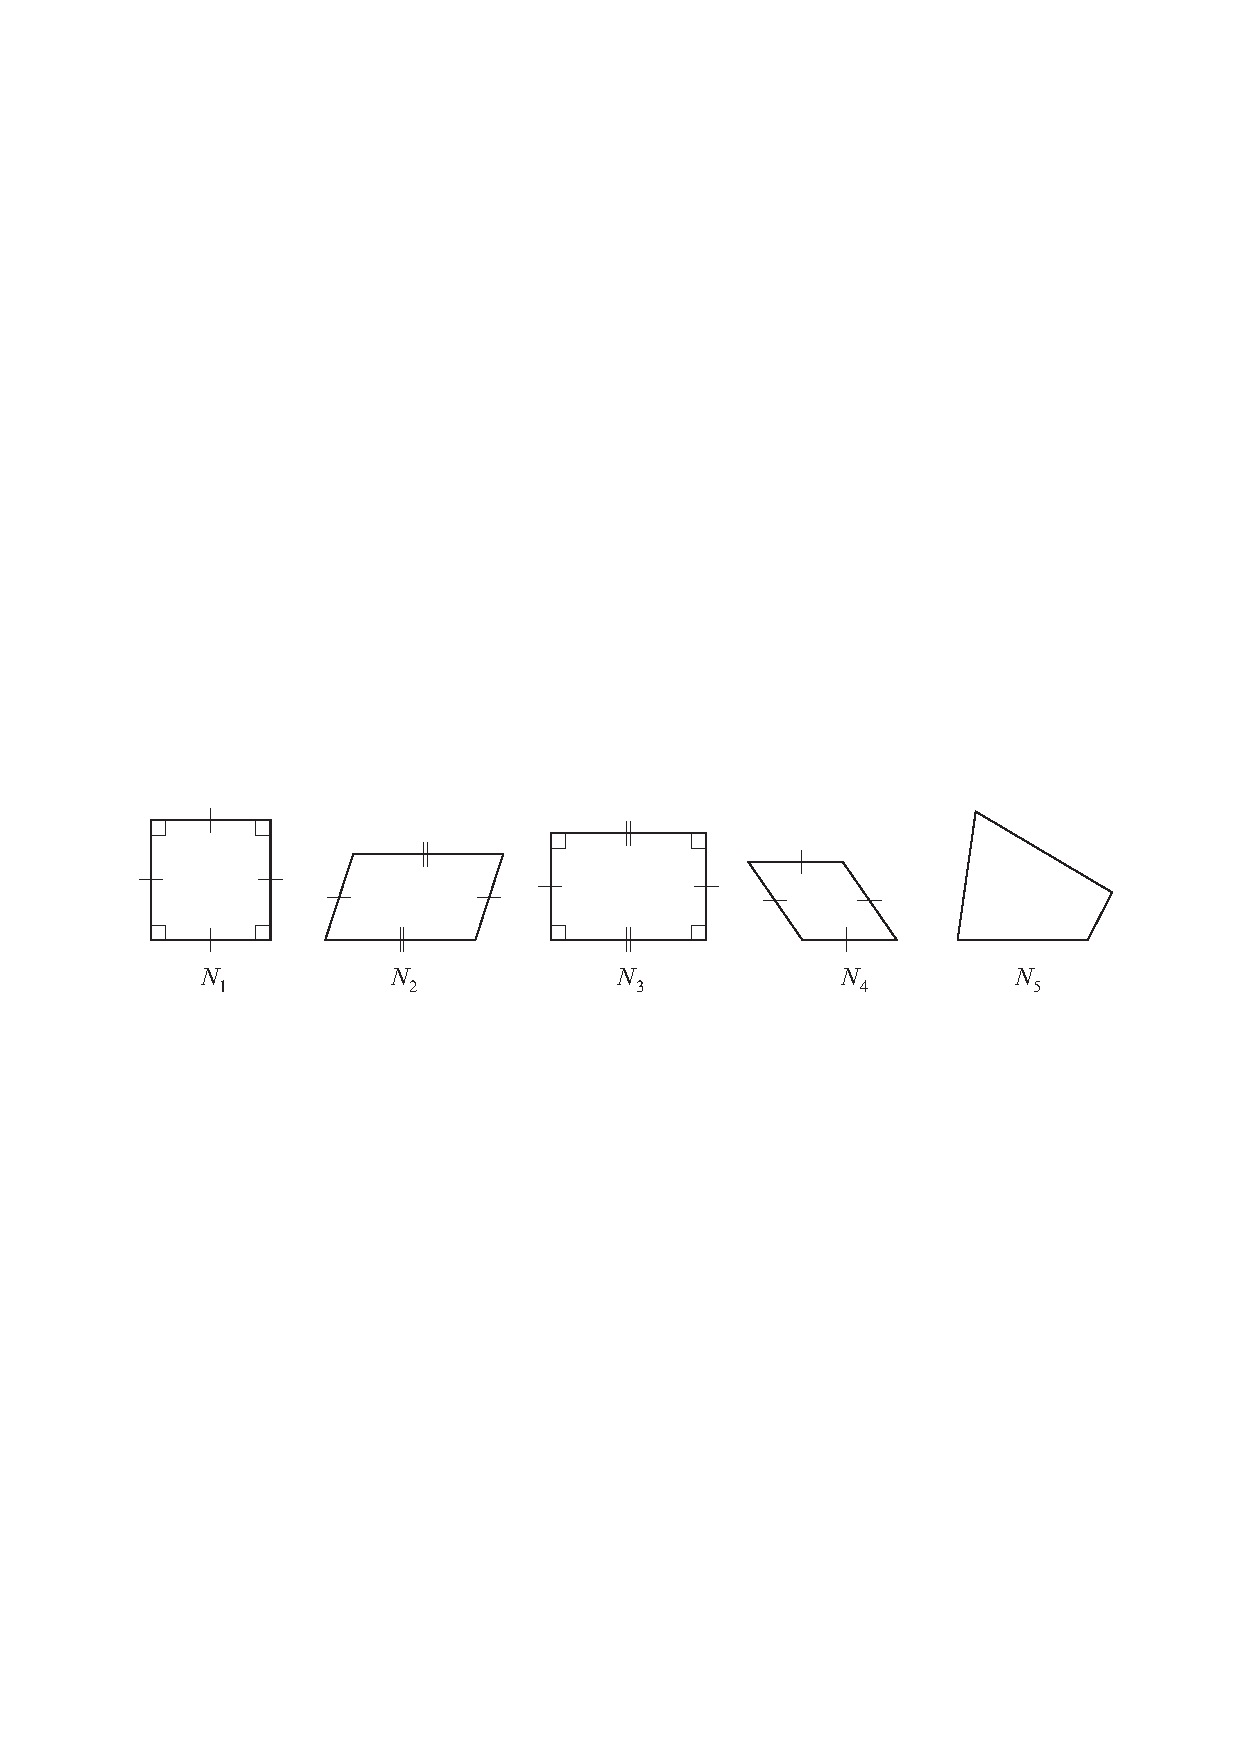
\includegraphics[width=12cm,height=4cm]{kuvat/Kappale3_2_esim_3_kuvio_v2}
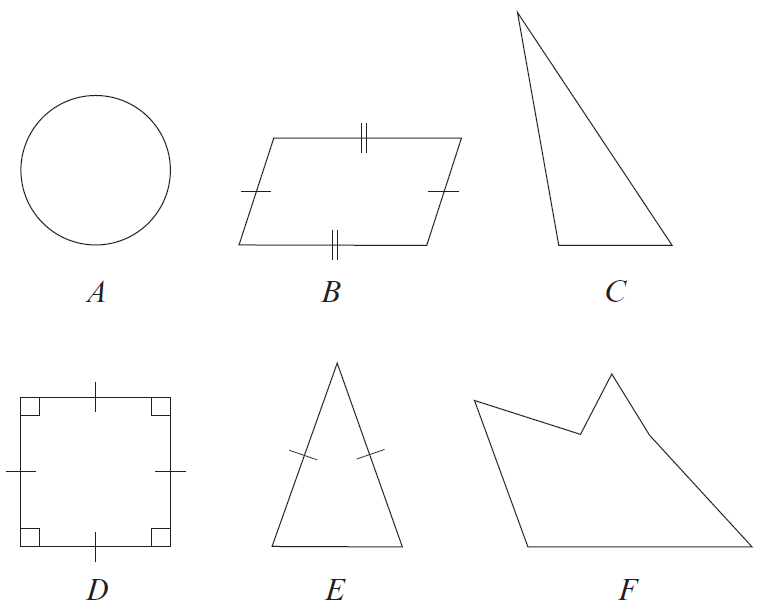
\includegraphics[width=8cm]{kuvat/kpl3_2_teht7}
\end{center}

\item
Olkoot $S(x)$ avoin lause ''kuvio $x$ on symmetrinen
jonkin suoran suhteen'' ja $P(x)$ avoin lause ''kuvio $x$
on symmetrinen jonkin pisteen suhteen''. Perusjoukon
muodostavat oheiset kuviot. Ratkaise avoin lause.
\begin{itemize}
\item[a)] $S(x)$,
\item[b)] $P(x)$,
\item[c)] $\lnot (S(x) \lor P(x))$,
\item[d)] $S(x) \lequiv P(x)$.
\end{itemize}




\item
Arvotaan kaksi lukua, joista molemmat voivat olla 1, 2 tai 3. Arvonnan tuloksena saadaan lukupari $(x, y)$, missä $x$ on ensimmäisen arvonnan tulos ja $y$ toisen arvonnan tulos. Olkoot avoimet lauseet $S(x, y)$: ''$x \le y$'' ja $T(x, y)$: ''tulo $xy$ on jaollinen luvulla 3''. Ratkaise avoin lause, kun perusjoukon muodostavat arvonnan tuloksena saatavat mahdolliset lukuparit
\[
(1, 1),\ (1, 2),\ (1, 3),\ (2, 1),\ (2, 2),\ (2, 3),\ (3, 1),\ (3, 2),\ (3, 3).
\]
\begin{itemize}
\item[a)] $S(x, y)$,
\item[b)] $\lnot T(x, y)$,
\item[c)] $\lnot (S(x, y) \lor T(x, y))$,
\item[d)] $S(x, y) \to T(x, y)$.
\end{itemize}

\item
Ratkaise reaalilukujen joukossa
\begin{itemize}
\item[a)] epäyhtälö $x^2 \le 4$,
\item[b)] epäyhtälöpari
\[
\left\{
\begin{array}{rcl}
x^2 & \le & 4 \\
x & > & -1.
\end{array}\right.
\]
\end{itemize}

\item
Ratkaise reaalilukujen joukossa epäyhtälö
\begin{itemize}
\item[a)] $|x| > 5$,
\item[b)] $|x| \le 1$,
\item[c)] $|x - 4| > 5$,
\item[d)] $|2x - 6| \le 1$.
\end{itemize}

\item Ratkaise avoin lause reaalilukujen joukossa. Ilmaise ratkaisujoukko myös välimerkintää käyttäen.
\begin{itemize}
\item[a)] $(x^2 > 1) \lor (0 \le x \le 2)$,
\item[b)] $(x^2 > 1) \land (0 \le x \le 2)$,
\item[c)] $(x^2 > 1) \to (0 \le x \le 2)$.
\end{itemize}

\item
Olkoot $P(x)$ avoin lause $(x < 10) \land (x^2 = 100)$ ja
$Q(x)$ avoin lause $(x \ge 10) \lequiv (x^2 = 100)$. Ratkaise avoin lause reaalilukujen joukossa.
\begin{itemize}
\item[a)] $P(x)$,
\item[b)] $Q(x)$,
\item[c)] $P(x) \lor Q(x)$,
\item[d)] $P(x) \land Q(x)$.
\end{itemize}


\end{enumerate}

{\bf Kotitehtäviä.}

\begin{enumerate}

\item
Olkoon $T(x,y)$ avoin lause ''$x$ lähettää tekstiviestin
$y$:lle''. Suomenna lause.
\begin{itemize}
\item[a)] $T(\textrm{Tiina}, \textrm{Elias})$,
\item[b)] $\lnot T(\textrm{Elias}, \textrm{Tiina}) \land T(\textrm{Elias}, \textrm{Vilma})$,
\item[c)] $T(x, x)$,
\item[d)] $T(y, \textrm{Rasmus}) \lequiv T(\textrm{Rasmus}, y)$.
\end{itemize}

\item
Olkoot $E(x)$ avoin lause ''$x$ on eurooppalainen
pääkaupunki'' ja $S(x)$ avoin lause ''$x$ on suomalainen
kaupunki''. Ratkaise avoin lause, kun perusjoukko on
$\{\textrm{Helsinki}, \textrm{Rovaniemi}, \textrm{Praha}, \textrm{Milano}\}$.
\begin{itemize}
\item[a)] $E(x)$,
\item[b)] $\lnot S(x)$,
\item[c)] $S(x) \land \lnot E(x)$,
\item[d)] $\lnot (E(x) \land S(x))$,
\item[e)] $E(x) \lequiv S(x)$.
\end{itemize}

\item
Olkoon $R(x)$ avoin lause ''$x^2 - 100 > 0$''. Onko lause
a) $R(10)$ b) $R(-15)$ tosi?

\item
Olkoon $S(x, y)$ avoin lause ''$x^2 + y^2 = 5$''. Onko
lause a) $S(2, 3)$ b) $S(2, -1)$ c) $S(-\sqrt{5}, 0)$ d)
$S(-1, -1)$ tosi?

\item
Ratkaise avoin lause $9x^2 + 30x + 25 \le 0$, kun
määrittelyjoukko on a) reaalilukujen joukko b)
kokonaislukujen joukko.

\item
Olkoot perusjoukko $\{ 1, 2, 3, \ldots , 16\}$, $C(x)$
avoin lause ''luku 12 on jaollinen luvulla $x$'' ja $D(x)$ avoin lause ''luvun $x$ neliöjuuri on kokonaisluku''.
Ratkaise avoin lause.
\begin{itemize}
\item[a)] $C(x)$,
\item[b)] $D(x)$,
\item[c)] $\lnot C(x) \land D(x)$,
\item[d)] $C(x) \lequiv D(x)$.
\end{itemize}

\item
Arvotaan kolme lukua, joista jokainen voi olla 1 tai
2. Arvonnan tuloksena saadaan lukukolmikko $(x, y, z)$, missä $x$ on ensimmäisen arvonnan tulos, $y$ toisen arvonnan tulos ja $z$ kolmannen arvonnan tulos. Olkoot
avoimet lauseet $S(x, y, z)$: ''$x + y + z \ge 5$'', $T(x,
y, z)$: ''tulo $xyz$ on pariton'' ja $U(x, y, z)$: “summa
$x + y + z$ on jaollinen luvulla 3''. Ratkaise avoin
lause, kun perusjoukon muodostavat arvonnan tuloksena
saatavat mahdolliset lukukolmikot
\[
(1, 1, 1),\ (1, 1, 2),\ (1, 2, 1),\ (1, 2, 2),\ (2, 1, 1),\ (2, 1, 2),\ (2, 2, 1),\ (2, 2, 2).
\]
\begin{itemize}
\item[a)] $S(x, y, z)$,
\item[b)] $T(x, y, z)$,
\item[c)] $U(x, y, z)$,
\item[d)] $S(x, y, z) \land T(x, y, z)$,
\item[e)] $S(x, y, z) \lor \lnot U(x, y, z)$,
\item[f)] $\lnot (S(x, y, z) \lor T(x, y, z) \lor U(x, y,z))$,
\item[g)] $S(x, y, z) \land (T(x, y, z) \lequiv U(x, y, z))$.
\end{itemize}

\item
Ratkaise reaalilukujen joukossa.
\begin{itemize}
\item[a)] $x^2 = 1$ tai $x(x + 5)(x - 1) = 0$
\item[b)] $x^2 = 1$ ja $x(x + 5)(x - 1) = 0$
\end{itemize}

\item
Ratkaise reaalilukujen joukossa
\begin{itemize}
\item[a)] epäyhtälö $x^2 - 11x + 30 > 0$,
\item[b)] epäyhtälöpari
\[
\left\{
\begin{array}{rcl}
x^2 - 11x + 30 & > & 0 \\
2x & > & -6 - x.
\end{array}\right.
\]
\end{itemize}

\item Ratkaise avoin lause reaalilukujen joukossa. Ilmaise ratkaisujoukko myös välimerkintää käyttäen.
\begin{itemize}
\item[a)] $(-4 < x) \lor (x < 8)$,
\item[b)] $(-4 < x) \land (x < 8)$,
\item[c)] $((-4 < x) \land (x < 8)) \land (-5 \le x \le -3)$,
\item[d)] $(-4 < x) \lequiv (-5 \le x \le -3)$.
\end{itemize}

\item
Olkoot $A(x)$ avoin lause $(x \ge 0) \to (x \ge 20)$
ja $B(x)$ avoin lause $\lnot ((x \le 0) \lor (x \ge 20))$. Ratkaise avoin lause reaalilukujen joukossa.
\begin{itemize}
\item[a)] $A(x)$,
\item[b)] $B(x)$,
\item[c)] $A(x) \lor B(x)$.
\end{itemize}

\end{enumerate}



\newpage

\subsection{Kvanttorit}
{\em Kvanttorien} avulla voidaan ilmaista täsmällisesti yleisluontoisia väitteitä, kuten tämän kirjan ensimmäisessä luvussa annettu esimerkki: ''kaikki joutsenet ovat valkoisia''. Tavoitteena on muodostaa loogisesti päteviä päätelmiä, jotka koskevat esimerkiksi jonkin joukon kaikkia alkioita.

\subsection*{Tutkimustehtävä}
Ovatko seuraavat väitteet tosia?
\begin{enumerate}
\item Kaikki koulumme opiskelijat opiskelevat englantia.
\item Kaikki koulumme opiskelijat opiskelevat pitkää matematiikkaa.
\item Koulussamme on opiskelija, joka harrastaa kilpaurheilua.
\item Koulussamme on opiskelija, joka on tämän vuoden Miss Suomi.
\item Kirjoita kohtien 1 ja 3 väitteiden negaatiot kahdella eri tavalla. 
\end{enumerate}

Predikaattilogiikassa määritellään kaksi kvanttoria, $\exists$ ja $\forall$. Näistä ensimmäistä kutsutaan {\em eksistenssikvanttoriksi} eli {\em olemassaolokvanttoriksi}. Lause
\[
\exists x\, P(x)
\]
tarkoittaa, että perusjoukossa $X$ on ainakin yksi alkio, jolla on ominaisuus $P$. Toisin sanoen joukko $P$ ei ole tyhjä joukko. Lause luetaan: ''On olemassa $x$ siten, että $P(x)$''.

Kvanttoria $\forall$ kutsutaan {\em universaalikvanttoriksi} eli {\em kaikkikvanttoriksi}. Lause
\[
\forall x\, P(x)
\]
tarkoittaa, että ominaisuus $P$ on kaikilla perusjoukon $X$ alkioilla. Lause luetaan: ''Kaikille $x$ pätee $P(x)$''.

Kvanttorien avulla voidaan esittää matemaattisia väittämiä hyvin tiiviissä ja täsmällisessä muodossa. Tästä on hyötyä etenkin matemaattisessa logiikassa, jossa tutkimuskohteena ovat matemaattiset teoriat, tulokset ja todistukset. 

{\bf Esimerkki 1.} Liikuntailtapäivässä koulun opiskelijat harrastavat eri talviurheilulajeja. Olkoot perusjoukko koulun opiskelijat ja avoimet lauseet $H(x)$: ''opiskelija $x$
 hiihtää'' ja $L(x)$: ''opiskelija $x$ laskettelee lumilaudalla''.

Kirjoita suomen kielellä lauseet a) $\forall x H(x)$,  b)  $\exists x L(x)$. Milloin lause on tosi? Milloin lause on epätosi?

{\bf Ratkaisu:} a) Lause tarkoittaa, että kaikki koulun opiskelijat hiihtävät. Lause on tosi silloin, kun
kaikki opiskelijat hiihtävät. Lause on epätosi silloin, kun on ainakin yksi opiskelija, joka ei 
hiihdä.  

b) Lause tarkoittaa, että joku koulun opiskelija laskettelee lumilaudalla. Lause on tosi
silloin, kun ainakin yksi opiskelija laskettelee lumilaudalla. Lause on epätosi silloin, kun 
kukaan koulun opiskelijoista ei laskettele lumilaudalla. 

{\bf Esimerkki 2.}
Olkoot perusjoukko reaalilukujen joukko $\mathbb{R}$ ja avoimet lauseet  $P(x)$: ''$x^2 > 0$''  sekä  
$Q(x)$: ''$x^2\le  0$''. Suomenna lauseet  a) $\forall x P(x)$,   b) $\exists x Q(x)$. Ovatko lauseet tosia?

{\bf Ratkaisu:}	a) Lause tarkoittaa, että kaikkien reaalilukujen neliöt ovat positiivisia. Lause on epätosi, sillä luvun $0$ neliö ei ole positiivinen: $0^2=0$.

Lauseen epätodeksi osoittamiseen siis riittää, että on olemassa yksikin alkio (niin sanottu {\em vastaesimerkki}), jolle avoin lause $P(x)$ on epätosi.

b)  Lause tarkoittaa, että on olemassa reaaliluku, jonka neliö on pienempi tai 
yhtä suuri kuin nolla. Lause on tosi, sillä $0^2 = 0$.

Lauseen todeksi osoittamiseen siis riittää, että on olemassa yksikin alkio, jolle avoin lause $Q(x)$ on tosi.

{\bf Vastaus:}	
a) Kaikkien reaalilukujen neliöt ovat positiivisia. Lause on epätosi.

b) On olemassa reaaliluku, jonka neliö on pienempi tai yhtä suuri kuin nolla. Lause on tosi. 


{\bf Esimerkki 3.}
Onko lause tosi? Perustele.
\begin{itemize}
\item[a)] $\exists x\in \Z(4x - 3 = 0)$
\item[b)] $\forall x\in \R(-x^2 + x \le 2)$
\end{itemize}

{\bf Ratkaisu:}

a) Yhtälön $4x - 3 = 0$ ratkaisu on $x = \frac{3}{4}$. Koska luku $\frac{3}{4}$ ei ole kokonaisluku, lause $\exists x\in \Z(4x - 3 = 0)$ on epätosi.

b) Epäyhtälö $-x^2+x \le 2$ on yhtäpitävä epäyhtälön $0 \le x^2 - x + 2$ kanssa. Tutkitaan polynomifunktion $x^2 - x + 2$ merkkiä. Ratkaistaan funktion $x^2 - x + 2$ nollakohdat toisen asteen yhtälön ratkaisukaavalla.
\[
x^2 - x + 2 = 0
\]
\[
x=\frac{-(-1) \pm \sqrt{(-1)^2 -4\cdot 1 \cdot 2}}{2 \cdot 1}=\frac{1 \pm \sqrt{-7}}{2}
\]
Funktiolla ei ole nollakohtia, koska diskriminantti $-7$ on negatiivinen. 

\begin{center}
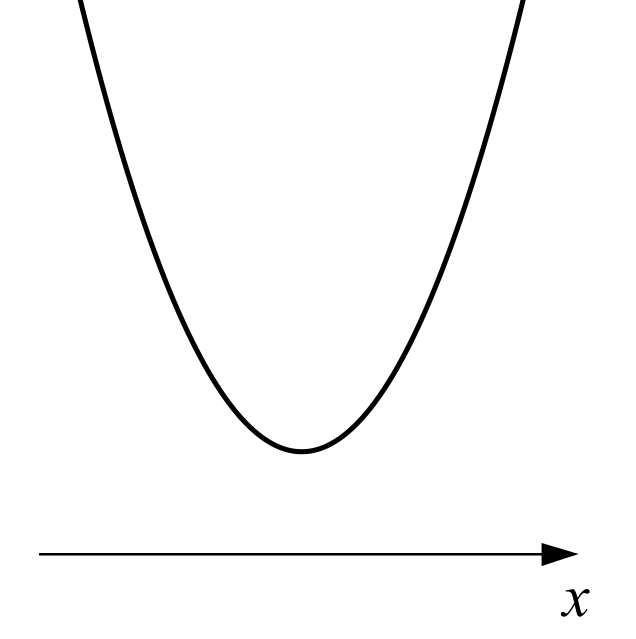
\includegraphics[width=5cm]{kuvat/kpl3_3_paraabeli}
\end{center}

Koska funktion $x^2 - x + 2$ kuvaaja on ylöspäin aukeava paraabeli, funktio saa vain positiivisia arvoja. Siten epäyhtälö $0 \le x^2 - x + 2$ toteutuu kaikilla muuttujan $x$ arvoilla. Lause $\forall x\in \R(-x^2 + x \le 2)$ on siis tosi.

{\bf Vastaus:} a) Lause on epätosi. b) Lause on tosi.

{\bf Esimerkki 4.}
Suomenna lause
\begin{itemize}
\item[a)] $\forall x\in \Z\exists y\in \Z (x+y=0)$
\item[b)] $\exists y\in \R\forall x\in \R (x+y =x)$.
\end{itemize}
Onko lause tosi?

{\bf Ratkaisu:}

a) Lause tarkoittaa, että jokaista kokonaislukua $x$ kohden on
olemassa sellainen kokonaisluku $y$, että lukujen summa on nolla.

Lause on tosi, sillä jokaisella kokonaisluvulla on vastaluku,
joka on kokonaisluku. Luvun ja sen vastaluvun summa on nolla.

b) Lause tarkoittaa, että on olemassa sellainen reaaliluku $y$,
että sen ja minkä tahansa reaaliluvun $x$ summa on aina yhtä
suuri kuin $x$.

Lause on tosi, sillä nolla on tällainen reaaliluku.

{\bf Vastaus:} a) Jokaista kokonaislukua $x$ kohden on olemassa
sellainen kokonaisluku $y$, että lukujen summa on nolla. Lause on
tosi.

b) On olemassa sellainen reaaliluku $y$, että sen ja minkä
tahansa reaaliluvun $x$ summa on aina $x$. Lause on tosi.


{\bf Kvanttorien negaatiot.} Tutkitaan lausetta ''kaikki joutsenet ovat valkoisia''. Lause voidaan formalisoida kaikkikvanttorin avulla $\forall x V(x)$, missä perusjoukkona on joutsenten joukko $J$ ja $V(x)$ on lause ''$x$ on valkoinen''. Tämä lause osoittautui epätodeksi, kun Australiasta löydettiin mustia joutsenia. Lauseen $\forall x V(x)$ negaatio $\lnot \forall x V(x)$ voidaan kirjoittaa $\exists x \lnot V(x)$ ja suomentaa ''on olemassa (ainakin yksi) joutsen, joka ei ole valkoinen''. Vastaavasti lauseen $\exists x V(x)$ negaatio $\lnot \exists x V(x)$ eli ''ei ole olemassa valkoista joutsenta'' voidaan lausua ekvivalentissa muodossa $\forall x \lnot V(x)$. Tämä lause voidaan hieman kömpelösti kielentää ''kaikki joutsenet ovat ei-valkoisia''.

%---
%{\bf Teorialaatikko [Kvanttorien negaatiot].} 
\fbox{
\begin{minipage}{12cm}
{\large \bf Kvanttorien negaatiot}

\medskip

Olkoon $P(x)$ avoin lause. Tällöin
\begin{itemize}
\item 
lause $\lnot \forall xP(x)$ on loogisesti ekvivalentti lauseen $\exists x\lnot P(x)$ kanssa, ja
\item
 lause $\lnot \exists xP(x)$ on loogisesti ekvivalentti lauseen $\forall x\lnot P(x)$ kanssa.
\end{itemize}
\end{minipage}
}
%---

Saatu kvanttorien negaatioita koskeva tulos muotoillaan joskus myös toisella tavalla. Koska lause $\lnot \forall x V(x)$ on loogisesti ekvivalentti lauseen $\exists x\lnot V(x)$ kanssa, voidaan päätellä, että lause $\forall x V(x)$ on loogisesti ekvivalentti lauseen $\lnot \exists x\lnot V(x)$ kanssa. Vastaava päättely voidaan tehdä myös eksistenssikvanttorin tapauksessa.



{\bf Esimerkki 5.}
Muodosta lauseen
\begin{itemize}
\item[a)] $\forall x \in \R(-x^2 \le 0)$
\item[b)] $\exists x\in \N(2x-3>0)$
\end{itemize}
negaatio. Onko negaatio tosi?

{\bf Ratkaisu:}

a) Lauseen $\forall x \in \R(-x^2 \le 0)$ negaatio on loogisesti ekvivalentti lauseen $\exists x\in \R (-x^2 > 0)$ kanssa.

Lause $\exists x\in \R (-x^2> 0)$ on epätosi, sillä tunnetusti $x^2$ on aina suurempi tai yhtä suuri kuin nolla. Siten $-x^2$ on aina pienempi tai yhtä suuri kuin nolla.

b) Lauseen $\exists x\in \N(2x-3>0)$ negaatio on loogisesti ekvivalentti lauseen $\forall x\in \N(2x-3 \le 0)$ kanssa.

Lause $\forall x\in \N(2x-3 \le 0)$ on epätosi, sillä esimerkiksi tapauksessa $x=5$ saadaan lausekkeen $2x - 3$ arvoksi $2\cdot 5 -3 = 7$, joka ei ole pienempi tai yhtä suuri kuin nolla.

{\bf Vastaus:} a) $\exists x\in \R (-x^2 > 0)$. Negaatio on epätosi. 

b) $\forall x\in \N(2x-3 \le 0)$. Negaatio on epätosi.



\newpage

\subsection*{Tehtäviä}

\begin{enumerate}

\item Olkoon perusjoukko kaikki koulun opiskelijat. Olkoon lause
$T(x)$: "opiskelija $x$ on täysi-ikäinen". Suomenna lause.
\begin{itemize}
\item[a)] $\forall x T(x)$
\item[b)] $\exists x T(x)$
\item[c)] $\exists x \lnot T(x)$
\item[d)] $\forall x \lnot T(x)$
\end{itemize}

\item Suomenna lause. Onko lause tosi? Perustele.
\begin{itemize}
\item[a)] $\forall x\in\R (|x| > 0)$
\item[b)] $\forall x\in\R (|x| \ge 0)$
\item[c)] $\exists x\in\N (x^2 < 2)$
\item[d)] $\exists x\in\N (x^2 = 2)$
\end{itemize}

\item
Formalisoi lause. Onko lause tosi? Perustele.
\begin{itemize}
\item[a)] Jokainen kokonaisluku on joko positiivinen tai
negatiivinen.
\item[b)] On olemassa sellainen kokonaisluku, jonka neliöjuuri on
yhtä suuri kuin luku itse.
\item[c)] Minkään kokonaisluvun neliö ei ole $7$.
\end{itemize}

\item Osoita, että yhtälö $\sqrt{x^2} = x$ ei pidä paikkaansa
kaikilla reaaliluvuilla.

\item Jalkapallojoukkue on lähdössä turnausmatkalle. Olkoon
$P(x,y)$ avoin lause "pelaajalla $x$ on pelaajan $y$
puhelinnumero". Suomenna lause.
\begin{itemize}
\item[a)] $\forall x \exists y P(x,y)$
\item[b)] $\exists x \forall y P(x,y)$
\item[c)] $\exists y \forall x P(x,y)$
\end{itemize}

\item
Formalisoi lause. Onko lause tosi?
\begin{itemize}
\item[a)] Positiivisten kokonaislukujen joukossa on pienin alkio.
\item[b)] Negatiivisten kokonaislukujen joukossa on pienin alkio.
\end{itemize}

\item Onko lause tosi? Perustele.
\begin{itemize}
\item[a)] $\forall x\in \R\exists y\in \R (xy=1)$
\item[b)] $\exists y\in \R\forall x\in \R (xy =x)$
\end{itemize}

\item Olkoon $M(x)$: "$x$ on matemaatikko". Formalisoi lause.

\begin{itemize}
\item[a)] Kaikki eivät ole matemaatikkoja.
\item[b)] Joku ei ole matemaatikko.
\item[c)] Ei ole olemassa matemaatikkoa.
\item[d)] Kukaan ei ole matemaatikko.
\end{itemize}

\item
Muodosta lauseen negaatio.
\begin{itemize}
\item[a)] $\forall x\in \Z (x < 12)$
\item[b)] $\exists x\in \Z (x^2 = 12)$
\item[c)] $\exists x\in \N ((x^2=9) \land (x<5))$
\item[d)] $\forall x\in \N ((x=0)\lor (x\ge 1))$
\end{itemize}

\item Osoita, että lause $\exists a,b,c \in \Z_{+} (a^2 + b^2 =
c^2)$ on tosi.

\item (Lisämateriaalia) Olkoot $M(x)$: "$x$ on matemaatikko" ja
$I(x)$: "$x$ on iloinen". Formalisoi lause.
\begin{itemize}
\item[a)] Kaikki ovat iloisia matemaatikkoja.
\item[b)] Matemaatikot ovat iloisia.
\item[c)] Kukaan matemaatikko ei ole iloinen.
\item[d)] Kaikki matemaatikot eivät ole iloisia.
\end{itemize}

\item (Lisämateriaalia) Olkoot $K(x)$: "$x$ on kampaaja" ja
$T(x,y)$: "$x$ tekee $y$:lle kampauksen". Formalisoi lause.
\begin{itemize}
\item[a)] Kukaan kampaaja ei tee kampausta itselleen.
\item[b)] Joku kampaaja tekee kampauksen niille kampaajille,
jotka eivät tee kampausta itselleen.
\end{itemize}

\end{enumerate}

{\bf Kotitehtäviä.}

\begin{enumerate}

\item Olkoon perusjoukko $xy$-tason suorien joukko. Olkoot
lauseet $N(x)$: "suora on nouseva" ja $L(x)$: "suora on laskeva".
Suomenna lause. Onko lause tosi?
\begin{itemize}
\item[a)] $\exists x L(x)$
\item[b)] $\forall x (N(x) \lor L(x))$
\item[c)] $\exists x (\lnot N(x) \land \lnot L(x))$
\item[d)] $\forall x \lnot N(x)$
\end{itemize}

\item Onko lause tosi? Perustele.
\begin{itemize}
\item[a)] $\forall x\in\R (x^2 \ge 0)$
\item[b)] $\exists x\in\N (x^2 = -9)$
\item[c)] $\forall x\in\R ((x-1)(x-3) \ge 0)$
\item[d)] $\exists x\in\Z (-x^2 - 2 \le 0)$
\end{itemize}

\item Onko lause tosi? Perustele.
\begin{itemize}
\item[c)] $\exists x\in \R (x^2 - 3x + 3 = 0)$
\item[d)] $\forall x\in \R (x^2 - 3x + 3 \ge 0)$
\end{itemize}

\item
\begin{itemize}
\item[a)] Osoita, että yhtälö $\sqrt{xy} = \sqrt{x}\sqrt{y}$ ei
pidä paikkaansa kaikilla reaaliluvuilla $x$ ja $y$.
\item[b)] Osoita, että on olemassa sellaiset reaaliluvut $x$ ja
$y$, että yhtälö $\sqrt{xy} = \sqrt{x}\sqrt{y}$ pitää paikkansa.
\item[c)] Millä ehdolla yhtälö $\sqrt{xy} = \sqrt{x}\sqrt{y}$
pitää yleisesti paikkansa?
\end{itemize}

\item Olkoon $S(x,y)$: "$x$ on suorittanut kurssin $y$".
Formalisoi lause.
\begin{itemize}
\item[a)] Joku on suorittanut kaikki kurssit.
\item[b)] Jokainen on suorittanut ainakin yhden kurssin.
\item[c)] Kukaan ei ole suorittanut kaikkia kursseja.
\item[d)] On olemassa kurssi, jota kukaan ei ole suorittanut.
\end{itemize}

\item Onko lause tosi? Perustele.
\begin{itemize}
\item[a)] $\forall x\in \Z_{+} \exists y\in \Z_{+} (x = \sqrt{y})
$
\item[b)] $\exists y\in \R \forall x\in \R (x^2 - 4 > y)$
\end{itemize}

\item Ilmaise suomen kielellä lauseen negaatio kahdella eri
tavalla soveltamalla kvanttorien negaatioiden loogisesti
ekvivalentteja muotoja.
\begin{itemize}
\item[a)] Jokainen opiskelija saa tästä kurssista arvosanan 10.
\item[b)] On olemassa opiskelija, joka saa tästä kurssista
arvosanan 10.
\end{itemize}

\item Kirjoita lause toisin.
\begin{itemize}
\item[a)] $\lnot \forall x \lnot P(x)$
\item[b)] $\lnot \exists x (P(x) \lor Q(x))$
\end{itemize}

\item
Muodosta lauseen negaatio. Onko negaatio tosi?
\begin{itemize}
\item[a)] $\forall x\in ]1, \infty [ (\sqrt{x} < x)$
\item[b)] $\exists x\in \Q (x^3 = 5)$
\item[c)] $\forall n \in \Z \exists m \in \Z ((n = 2m) \lor (n =
2m+1))$
\end{itemize}

\item Funktiota $f\colon X\to Y$ voidaan ajatella kahden
muuttujan avoimena lauseena $P(x,y)$: "$f(x) = y$", missä
$x$ kuuluu määrittelyjoukkoon $X$ ja $y$ maalijoukkoon $Y$.
Funktiolta edellytetään lisäksi, että
\begin{itemize}
\item $\forall x \exists y P(x,y)$, ja
\item $\lnot (\exists x \exists y \exists z (P(x,y) \land P(x,z)
\land (y \neq z)))$.
\end{itemize}
Tulkitse sanallisesti tai kuvaa käyttäen, mitä tämä määritelmä
tarkoittaa.

\item (Lisämateriaalia) Olkoot $S(x,y)$: "$x$ on suorittanut
kurssin $y$" ja $L(x)$: "$x$ on lukiolainen". Formalisoi lause.
\begin{itemize}
\item[a)] Joku lukiolainen on suorittanut kaikki kurssit.
\item[b)] Kukaan lukiolainen ei ole suorittanut kaikkia kursseja.
\end{itemize}

\item (Lisämateriaalia) Olkoot $S(x,y)$: "$x$ on suorittanut
kurssin $y$", $L(x)$: "$x$ on lukiolainen" ja $M(y)$: "$y$ on
pitkän matematiikan kurssi". Formalisoi lause.
\begin{itemize}
\item[a)] Joku lukiolainen ei ole suorittanut yhtään pitkän
matematiikan kurssia.
\item[b)] Joku lukiolainen on suorittanut pitkän matematiikan
kurssin.
\item[c)] Jokaisella lukiolaisella on pitkän matematiikan kurssi
suoritettuna.
\item[d)] On olemassa pitkän matematiikan kurssi, jota kukaan
lukiolainen ei ole suorittanut.
\end{itemize}

\item (Lisämateriaalia) Määritä kaikki funktiot $f\colon X\to Y$,
kun $X=\{a,b,c\}$ ja $Y=\{1,2\}$.

\item (Lisämateriaalia) Määritä kaikki funktiot $f\colon X\to Y$,
kun $X=\emptyset$ ja $Y\neq \emptyset$.

\item (Lisämateriaalia) Määritä kaikki funktiot $f\colon X\to Y$,
kun $X\neq \emptyset$ ja $Y= \emptyset$.

\item (Lisämateriaalia) Tutustu logiikkapohjaiseen Prolog-
ohjelmointikieleen\\
\href{http://www.cs.helsinki.fi/u/wikla/OKP/OppaatK07/
prolog.html}
{{\tt http://www.cs.helsinki.fi/u/wikla/OKP/OppaatK07/
prolog.html}}

Lataa koneellesi Prolog-tulkki \href{http://www.gprolog.org/}
{{\tt http://www.gprolog.org/}}
ja kokeile Prolog-ohjelmointia.

\end{enumerate}

\newpage

\section{Matemaattisen väitteen todistaminen}

Matematiikassa pyritään {\em todistamaan} matemaattisia tuloksia. Todistamisen ideana on, että tulos johdetaan loogisesti sitovalla päättelyllä, jossa voidaan vedota aikaisemmin todistettuihin tuloksiin, käsiteltävän teorian {\em aksioomiin} eli perusoletuksiin sekä loogisiin päättelysääntöihin. Matematiikassa tärkeimpiä tuloksia sanotaan yleensä {\em lauseiksi} eli {\em teoreemoiksi} (esim. Pythagoraan lause) ja pienempiä aputuloksia kutsutaan {\em apulauseiksi} eli {\em lemmoiksi}.

Kun tulos on todistettu matemaattisesti, se on kumoamaton. Matemaattiset tulokset eivät siksi vanhene. Toisaalta matemaattisten tulosten soveltamista rajoittavat niiden johtamisessa käytetyt oletukset, koska tulos ei sano mitään tilanteesta, jossa nämä oletukset eivät ole voimassa.

\subsection*{Tutkimustehtävä}
%Tutkitaan lukujen parillisuutta ja parittomuutta.
\begin{enumerate}
\item Mitä lukuja tarkoittaa merkintä $2n$, kun $n$ käy läpi kaikki luonnolliset luvut? Entä mitä lukuja tarkoittaa merkintä $2n + 1$, kun $n\in \mathbb{N}$?
\item %Kaikki parilliset luvut voidaan esittää muodossa $2n$, missä $n$ on kokonaisluku. Esimerkiksi $12=2\cdot 6$.
Esitä luvut $6$, $10$ ja $26$ muodossa $2n$.
\item %Kaikki parittomat luvut voidaan esittää muodossa $2n + 1$, missä $n$ on kokonaisluku. 
Esitä luvut $7$, $11$ ja $35$ muodossa $2n+1$.
%\item Laske yhteen parittomia lukupareja. Esimerkiksi $5 + 7 =12$. Mitä havaitset summasta? 
%Kahden parittoman luvun summa on aina \underline{\phantom{xxxxxxxxxx}}.
%\item Todista edellisessä kohdassa muotoilemasi väite käyttäen kohdissa (1) ja (2) esitettyjä parillisten ja parittomien lukujen esitysmuotoja.
%\item Todista väite matemaattisesti. Voit käyttää merkintöjä $2n$ ja $2n + 1$, $n\in\mathbb{N}$.
\item Laske yhteen parittomia lukuja. Esimerkiksi $5 + 7 = 12$. Mitä havaitset summasta?
\item Todista havainto matemaattisesti. Kahdelle eri suurelle parittomalle luvulle voidaan käyttää yleisiä merkintöjä $2n + 1$, $n \in\N$, ja $2m + 1$, $m \in\N$.
\end{enumerate}

%\subsection*{Tutkimustehtävä}
%\begin{enumerate}
%\end{enumerate}

{\bf Oletus, väite ja deduktio}

% (formaaleja väittämiä, suora todistus,vastaesimerkkitodistus, tehtäviä oletusten ja väitteiden)
Matemaattinen tulos muodostuu kolmesta osasta. Tulokseen liittyy {\em oletuksia}. Oletusten täytyy olla tosia, jotta tulosta voitaisiin käyttää. Tuloksen toinen osa on {\em väite}. Matematiikan lause sanoo, että oletusten vallitessa lauseen väite on myös tosi. Tuloksen kolmas osa on {\em todistus}. Matemaattinen todistus on deduktiivinen päättelyketju, jossa oletuksista johdetaan lauseen väite. Matemaattisen todistuksen loppuun merkitään yleensä pieni neliö merkiksi todistuksen päättymisestä.

Yksinkertaisin matemaattisen todistuksen tyyppi on {\em suora todistus}. Suorassa todistuksessa tulos saadaan suoralla päättelyllä, jossa voidaan vedota lauseen oletuksiin, aksioomiin, määritelmiin ja aikaisemmin todistettuihin tuloksiin, esimerkiksi laskusääntöihin. Suoralla todistuksella voidaan todistaa seuraavan esimerkin tulos.

{\bf Esimerkki 1.} Todista lause.

{\bf Lause 1.} Olkoot $m$ ja $n$ parillisia kokonaislukuja. Tällöin luku $m+n$ on parillinen.

\proof
Koska $m$ ja $n$ ovat parillisia, voidaan kirjoittaa $m=2a$ ja $n=2b$, missä $a$ ja $b$ ovat kokonaislukuja.

Siten
\[
m+n =2a+2b = 2(a+b).
\]

Luku $2(a+b)$ on parillinen, joten väite on todistettu.
\qed

{\bf Esimerkki 2.} Todista lause.

{\bf Lause 2.} Kahden rationaaliluvun summa on rationaalinen.

\proof
Olkoot $q_1$ ja $q_2$ kaksi rationaalilukua. Ne voidaan kirjoittaa muodossa
\[
q_1=\frac{m_1}{n_1},\qquad 
q_2=\frac{m_2}{n_2},
\]
ja missä $m_1,m_2,n_1,n_2$ ovat kokonaislukuja ja $n_1,n_2\neq 0$.

Edelleen voidaan kirjoittaa
\[
q_1+q_2 = \frac{m_1}{n_1}+ \frac{m_2}{n_2}
\]
\[
= \frac{m_1 n_2}{n_1 n_2}+ \frac{m_2 n_1}{n_2 n_1} = \frac{m_1n_2 + m_2 n_1}{n_1 n_2}.
\]

Nyt $m_1n_2 + m_2 n_1$ sekä $n_1 n_2$ ovat kokonaislukuja ja $n_1 n_2\neq 0$, joten summa $q_1+q_2$ kuuluu rationaalilukujen joukkoon $\mathbb{Q}$.
\qed

{\bf Esimerkki 3.} Todista lause.

{\bf Lause 3.} Olkoot $a$ ja $b$ reaalilukuja. Tulo $ab<0$, jos ja vain jos joko $a>0$ ja $b<0$ tai $a<0$ ja $b>0$.

\proof
Ekvivalenssilauseen väite on muotoa ''jos ja vain jos''. Tällainen lause todistetaan usein kahdessa osassa.

Todistetaan aluksi lauseen ''jos''-osa: $ab<0$, jos joko $a>0$ ja $b<0$ tai $a<0$ ja $b>0$.

Oletetaan aluksi, että $a>0$ ja $b<0$. Kertomalla epäyhtälö $b<0$ luvulla $a$ saadaan $ab<0$.

Vastaavasti jos $a<0$ ja $b>0$, niin kertomalla epäyhtälö $a<0$ luvulla $b$ saadaan $ab<0$. Siten lauseen ensimmäinen osa on todistettu.

Osoitetaan seuraavaksi lauseen toinen osa: $ab<0$ vain, jos $a>0$ ja $b<0$ tai $a<0$ ja $b>0$.

Huomataan aluksi, että jos $ab<0$, niin $a\neq 0$ ja $b\neq 0$. Jos $a>0$, niin jakamalla epäyhtälö $ab<0$ luvulla $a$ saadaan $b<0$. Toisaalta, jos $a<0$, niin jaettaessa epäyhtälön $ab<0$ suunta vaihtuu ja saadaan $b>0$. Siis myös lauseen toinen osa on todistettu.
\qed

{\bf Epäsuora todistus}
%{\bf (mainittava ristiriitatodistus; yleinen ristiriita ja käänteinen todistus; väitteen negaatioon)}
Tärkeä esimerkki matemaattisesta todistusmenetelmästä on {\em epäsuora todistus}. Epäsuora todistus perustuu jo aikaisemmin tässä kurssissa esiintyneeseen kolmannen poissulkevan lakiin. Tämä laki sanoo, että kaikki väitteet ovat joko tosia tai epätosia.

{\em Käänteisessä todistuksessa} ajatuksena on, että väitteen $A\to B$ todistamiseksi riittää osoittaa, että väitteen $B$ negaatio $\lnot B$ eli niin sanottu {\em vastaoletus} johtaa oletuksen $A$ negaatioon $\lnot A$. Käänteinen todistus perustuu kappaleessa 2.3 esiteltyyn kontraposition lakiin, jonka mukaan lauseet $A\to B$ ja $\lnot B \to \lnot A$ ovat loogisesti ekvivalentit. 

Käänteisessä todistuksessa täytyy siis olettaa väitteen negaatio ja päätellä siitä, että oletus on epätosi. Tällä tavoin voidaan osoittaa esimerkiksi seuraava tulos:

{\bf Lause 4.} Olkoon $m\in \N$ siten, että $m^2$ on parillinen. Tällöin $m$ on parillinen.

\proof
Lauseen todistamiseksi tehdään vastaoletus, joka on lauseen väitteen ''$m$ on parillinen'' negaatio.

Vastaoletus: $m$ on pariton.

Tästä seuraa, että on olemassa $k\in \N$, jolle $m=2k+1$.

Nyt
\[
m^2 = (2k+1)^2 = 4k^2+4k+1 = 2(2k^2+2k)+1.
\]

Siten $m^2$ on pariton. On päädytty ristiriitaan lauseen oletuksen kanssa. Siten lauseen väite on tosi.
\qed

{\em Ristiriitatodistuksessa} pyritään todistamaan muotoa $A\to B$ oleva väite tekemällä ensin vastaoletus $\lnot B$ ja päätymällä johonkin ristiriitaan, ei kuitenkaan välttämättä oletuksen $A$ negaatioon.

Ehkä kuuluisin esimerkki epäsuorasta todistuksesta on todistus sille, että luku $\sqrt{2}$ on irrationaalinen. Todistuksessa tarvitaan seuraavaa lisätietoa rationaaliluvuista. Sanotaan, että kokonaisluku $a$ on kokonaisluvun $b$ {\em tekijä}, jos on olemassa sellainen kokonaisluku $c$, että $b=a\cdot c$. Rationaaliluku $q\in\Q$ voidaan aina esittää {\em supistetussa muodossa} $q=m/n$, missä $m$ ja $n$ ovat kokonaislukuja, joilla ei ole yhteisiä tekijöitä, ja $n\neq 0$. Esimerkiksi murtoluku $2/5$ on supistetussa muodossa, koska luvuilla $2$ ja $5$ ei ole yhteisiä tekijöitä. Sen sijaan murtoluku $6/9$ ei ole supistetussa muodossa, koska luku $3$ on sekä osoittajan että nimittäjän tekijä. Murtoluvun $6/9$ esitys supistetussa muodossa on $2/3$.

{\bf Lause 5.} Luku $\sqrt{2}$ on irrationaalinen.

\proof
Vastaoletus: Luku $\sqrt{2}$ on rationaalinen.

On siis olemassa luku $q\in \Q$ siten, että $q^2=2$.

Kirjoitetaan luku $q$ supistetussa muodossa $q=m/n$, missä kokonaisluvuilla $m$ ja $n$ ei ole yhteisiä tekijöitä. Nyt $q^2=2$, jos ja vain jos
\[
\bigg(\frac{m}{n}\bigg)^2=2.
\]

Kertomalla puolittain luvulla $n^2$ saadaan yhtälö
\[
m^2 = 2n^2.
\]

Koska luku $2n^2$ on parillinen, on $m^2$ parillinen. Lauseen 4 perusteella myös $m$ on parillinen.

Siten on olemassa $k\in \Z$, jolle $m=2k$.

Koska
\[
n^2=m^2/2=(2k)^2/2= 2k^2,
\]
luku $n^2$ on parillinen. Lauseen 4 nojalla myös $n$ on parillinen.

Näin ollen luku $2$ on lukujen $m$ ja $n$ yhteinen tekijä. Tämä on ristiriita, koska oletettiin, ettei näillä luvuilla ole yhteisiä tekijöitä.
\qed

\newpage




\subsection*{Tehtäviä}

\begin{enumerate}

\item a) Laske neljän peräkkäisen kokonaisluvun summa.
Toista lasku useilla neljän peräkkäisen kokonaisluvun
joukoilla. Mitä havaitset summasta?
b) Jos neljän peräkkäisen kokonaisluvun joukon pienin
luku on $m$, niin millainen esitysmuoto on kolmella
muulla luvulla?
c) Todista a-kohdan tulos matemaattisesti käyttäen
hyväksi b-kohdan esitysmuotoja.

\item Todista, että parillisen ja parittoman kokonaisluvun
summa on pariton.

\item Todista, että kahden parillisen kokonaisluvun tulo
on parillinen.

\item Todista, että kahden rationaaliluvun tulo on rationaalinen.

\item Olkoot $a$ ja $b$ kokonaislukuja. Todista, että luku
$a + b$ on parillinen silloin ja vain silloin, kun luku
$a - b$ on parillinen.

\item Olkoon $m$ sellainen kokonaisluku, että $m^2$ on
pariton. Todista, että tällöin $m$ on pariton.

\item Todista väite todeksi tai epätodeksi: Kahden
irrationaaliluvun summa on aina irrationaaliluku.

\item Luku $\sqrt{3}$ on irrationaaliluku. Todista,
että $\sqrt{3}+1/2$ on irrationaaliluku. Vihje: Käytä
epäsuoraa todistusta.

\item Todista, että irrationaaliluvun ja nollasta poikkeavan rationaaliluvun tulo on irrationaaliluku.

\item Todista, että luku $\sqrt{6}$ on irrationaaliluku.

\item Todista: Jos luku $a$ on irrationaaliluku, niin
myös luku
\[
\frac{2a-5}{3a-11}
\]
on irrationaaliluku. Vihje: Käytä symbolisen laskimen
{\tt solve}-toimintoa.

\item
Tarkastellaan suorakulmaista kolmiota, jonka kateettien
pituudet ovat $a$ ja $b$ ja hypotenuusan pituus $c$.
Todista väite todeksi tai epätodeksi.

\begin{itemize}
\item[a)] On olemassa sellainen suorakulmainen kolmio,
jonka sivujen pituudet $a$, $b$ ja $c$ ovat kaikki parillisia kokonaislukuja.
\item[b)] On olemassa sellainen suorakulmainen kolmio,
jonka sivujen pituudet $a$, $b$ ja $c$ ovat kaikki 
parittomia kokonaislukuja.
\end{itemize}

\item Kokonaisluvut $0, 1, 2, \ldots, 12$ asetetaan
mielivaltaiseen järjestykseen ympyrän kehälle. Todista,
että joidenkin neljän peräkkäisen luvun summa on
vähintään 26.

\end{enumerate}

{\bf Kotitehtäviä.}

\begin{enumerate}

\item
\begin{itemize}
\item[a)] Laske luonnollisten lukujen $1, 2, 3,\ldots,
10$ neliöt.
\item[b)] Esitä väite luonnollisten lukujen neliöiden
parillisuudesta tai parittomuudesta.
\item[c)] Todista väitteesi matemaattisesti.
\end{itemize}

\item Todista, että kolmen parittoman kokonaisluvun summa on pariton.

\item Todista, että kolmen peräkkäisen kokonaisluvun summa
on jaollinen luvulla 3.

\item Todista, että kahden parittoman kokonaisluvun tulo
on pariton.

\item Olkoot $a$ ja $b$ reaalilukuja. Todista, että tulo $ab = 0$, jos ja vain jos $a=0$ tai $b=0$.

\item Olkoon $n$ kokonaisluku. Todista, että luku $n^{2} + 3n + 1$ on aina pariton. Käytä a) suoraa b) epäsuoraa
todistusta.

\item Todista, että ei ole olemassa sellaisia
positiivisia kokonaislukuja $x$ ja $y$, jotka toteuttavat
yhtälön $4^{x} = 7^{y}$.

\item Todista väite todeksi tai epätodeksi: Kahden
irrationaaliluvun tulo voi olla rationaaliluku.

\item Todista, että luku $\sqrt{5}$ on irrationaaliluku.
Tarvitset seuraavaa lisätietoa: jos kahden kokonaisluvun
tulo on jaollinen luvulla 5, niin ainakin toinen tulon
tekijöistä on jaollinen luvulla 5.

\item Tarkastellaan paritonta määrää parittomia
kokonaislukuja. Todista, että lukujen keskiarvo ei voi
olla nolla.

\item Tarkastellaan kolmiota, jonka sivujen pituudet ovat
$a$, $b$ ja $c$. Niin sanotun {\em Heronin kaavan} mukaan
kolmion pinta-alalle pätee $A = \sqrt{p(p-a)(p-b)(p-c)}$,
missä $p = \frac{1}{2}(a+b+c)$. Todista, että jos kolmion
sivujen pituudet ovat luvulla 4 jaollisia kokonaislukuja,
niin kolmion pinta-alan neliö on jaollinen luvulla 16.

\item
Niin sanotun {\em Fermat'n suuren lauseen} mukaan ei ole
olemassa sellaisia positiivisia kokonaislukuja $x$, $y$
ja $z$, jotka toteuttaisivat yhtälön $x^{n} + y^{n} = z^{n}$, missä $n$ on lukua 2 suurempi kokonaisluku.
Erityisesti siis yhtälöllä $x^{3} + y^{3} = z^{3}$ ei
ole ratkaisua, jos $x$, $y$ ja $z$ ovat positiivisia
kokonaislukuja.
\begin{itemize}
\item[a)] Todista, että ei ole olemassa sellaisia
positiivisia rationaalilukuja $x$, $y$ ja $z$, jotka
toteuttavat yhtälön $x^{3} + y^{3} = z^{3}$.
\item[b)] Todista väite todeksi tai epätodeksi: ei ole
olemassa sellaisia keskenään eri suuria kokonaislukuja
$x$, $y$ ja $z$, jotka toteuttavat yhtälön $x^{3} + y^{3} = z^{3}$.
\end{itemize}

\item Olkoot $a$ ja $b$ reaalilukuja, joille pätee $0 \le a \le 1$ ja $0 \le b \le 1$. Todista, että tällöin $0 \le \frac{a + b}{1 + ab} \le 1$.

\end{enumerate}


\newpage

\section{Johdanto lukuteoriaan}

Kurssin loppuosassa perehdytään lukuteoriaan. Lukuteoria on matematiikan ala, joka tutkii kokonaislukuja. Lukuteorialla on nykyään paljon sovelluksia mm. tietotekniikassa ja digitaalisessa tiedonsiirrossa. Esimerkiksi yleisesti käytetty RSA-sala\-kir\-joi\-tus\-me\-ne\-tel\-mä perustuu lukuteorian tuloksiin. Lukuteoria tarjoaa myös havainnollisen johdannon moniin matemaattisiin ajattelutapoihin, joita käytetään myös muiden matemaattisten teorioiden yhteydessä.

{\bf Kuva: pankkiautomaatti.}

\subsection{Jaollisuus ja jakojäännös}
\label{jaollisuus}
Kokonaislukujen jaollisuus on lukuteoriassa keskeinen käsite, johon on tutustuttu jo alakoulussa.

\subsection*{Tutkimustehtävä} %Palautetaan mieliin jaollisuus ja jakojäännös.
\begin{enumerate}
\item
Laske jakokulmassa a) $905 / 11$ b) $540 / 12$. Ilmoita jakolaskun tulos kokonaisosan ja jakojäännöksen avulla.
\item
Kirjoita kummankin jakolaskun perusteella yhtälö, joka kertoo, kuinka jaettava saadaan
ilmaistua osamäärän, jakajan ja jakojäännöksen avulla.
\end{enumerate}


Alakoulun matematiikassa esimerkiksi kokonaislukujen jakolasku $17/3$ ratkaistaan seuraavasti: $17/3 = 5$, jää $2$. Tämä tarkoittaa, että luku $3$ menee $5$ kertaa lukuun $17$ ja jää $2$. Yleisesti kokonaislukujen $a$ ja $b \neq 0$ jakolaskusta $a/b$ saadaan tulokseksi {\em osamäärä} ja {\em jakojäännös}. Edellisessä jakolaskussa osamäärä on $5$ ja jakojäännös on $2$. Mikäli jakojäännös on nolla eli jako menee tasan, sanotaan, että luku $a$ on {\em jaollinen} luvulla $b$ tai että luku $b$ {\em jakaa} luvun $a$. Tällöin merkitään $b|a$. Jos $b|a$, niin luku $a$ voidaan kirjoittaa osamäärän $q$ ja luvun $b$ avulla $a = qb$. Itse asiassa nämä ehdot ovat yhtäpitäviä. Jos luku $a$ ei ole jaollinen luvulla $b$, merkitään $b \nmid a$.

{\bf Esimerkki 1.} Tutki, onko totta, että a)  $3 | 6$  b)  $2 | 5$ c) $-4|12$.

{\bf Ratkaisu:}

a) Tapa 1: Suoritetaan jakolasku $6/3= 2$. Jako menee tasan, joten luku $6$ on jaollinen luvulla $3$. Siis $3 | 6$.

Tapa 2: Koska $6 = 2 \cdot 3$, luku $3$ on luvun $6$ tekijä. Siis $3 | 6$.

b) Tapa 1: Suoritetaan jakolasku $5/2 = 2$, jää $1$. Jako ei mene tasan, joten luku $5$ ei ole jaollinen luvulla $2$. Siis $2 \nmid 5$.

Tapa 2: Lukua $5$ ei voida kirjoittaa muodossa $2q$, missä $q\in\Z$, sillä luku $5$ ei ole parillinen. Siis $2 \nmid 5$.

c) 
Tapa 1: Suoritetaan jakolasku $12/(-4)=-12/4= -3$. Jako menee tasan, joten luku $12$ on jaollinen luvulla $-4$. Siis $-4 | 12$.

Tapa 2: Koska $12 = -3 \cdot (-4)$, luku $-4$ on luvun $12$ tekijä. Siis $-4 | 12$.

{\bf Vastaus:} a) On.  b) Ei ole. c) On.


Jaollisuuden tutkimisessa tärkeä tulos on seuraava lause, jonka todistus on melko vaativa:

{\bf Lause (Jakoyhtälö).}
Jos $a$ ja $b$ ovat kokonaislukuja ja $b > 0$, niin on olemassa sellaiset yksikäsitteiset kokonaisluvut $q$ ja $r$, että
\[
a = qb + r,\qquad 0\le r<b.
\]
Jakoyhtälössä esiintyvää lukua $q$ sanotaan lukujen $a$ ja $b$ (vaillinaiseksi) osamääräksi ja lukua $r$  jakojäännökseksi.

%Jakojäännökselle käytetään myös merkintää 
%\[
%r = a \mod b.
%\]

\proof (Lisämateriaali)
Todistetaan väite tapauksessa $a\ge 0$. Tutkitaan aluksi joukkoja
\[
S = \{ a-nb\,|\, n\in \Z\}.
\]
Koska $a\in S$, tässä joukossa on ainakin yksi epänegatiivinen alkio. Olkoon $r=a-qb$ joukon $S$ pienin epänegatiivinen alkio. Nyt $r < b$, koska muuten luku 
\[
0\le r - b = a - qb - b = a - (q+1)b 
\]
olisi lukua $r$ pienempi joukon $S$ epänegatiivinen alkio.

Yksikäsitteisyyden toteamiseksi tehdään vastaoletus, että
\[
a= q_1b+r_1 = q_2b+r_2.
\]
Voidaan olettaa, että $q_2>q_1$. Nyt
\[
r_1 - r_2 = q_2b - q_1b = (q_2-q_1)b \ge b.
\]
Toisaalta $r_1-r_2<b$, koska $0\le r_1 < b$ ja $0\le r_2 < b$, mikä on ristiriita. Siten ainoa mahdollisuus on, että $q_1=q_2$ ja $r_1=r_2$. 
\qed


{\bf Esimerkki 2.}
%Määritä jakolaskun $a/b$ osamäärä ja jakojäännös, kun
%a) $a=23$ ja $b=5$, 
%b) $a=-19$ ja $b=6$. 
%Kirjoita vastaavat jakoyhtälöt.
Määritä jakolaskun osamäärä ja jakojäännös sekä kirjoita vastaava jakoyhtälö, kun
a) luku $23$ jaetaan luvulla $5$,  b)  luku $-19$ jaetaan luvulla $6$.

{\bf Ratkaisu:}
a) Vaillinainen osamäärä voidaan selvittää päässälaskulla tai laskinta käyttäen. Laskinta käytettäessä lasketaan jakolasku normaalisti ja otetaan lopputuloksen kokonaisosa.

Laskin antaa $23/5 = 4,6$, joten vaillinaiseksi osamääräksi saadaan $4$.

Jakojäännös saadaan nyt selville vähentämällä luku $4\cdot 5$ jaettavasta $23$, siis $23-4\cdot 5=3$. Siten jakojäännökseksi saadaan $3$. 
%Voidaan myös merkitä
%\[
%r=23 \mod 5 = 3.
%\]
Jakoyhtälö on
\[
23 = 4\cdot 5 + 3.
\]

b) Laskin antaa $-19/6 \approx -3,167$. Vaillinaiseksi osamääräksi on valittava $-4$, jotta jakojäännös olisi epänegatiivinen.

Jakojäännös saadaan jälleen selville vähentämällä luku $-4\cdot 6$ jaettavasta $-19$, siis $-19-(-4)\cdot 6=-19+24=5$. Siten jakojäännökseksi saadaan $5$. 
Jakoyhtälö on
\[
-19 = -4\cdot 6 +5.
\]

{\bf Vastaus:} a) $23 = 4\cdot 5 + 3$, b) $-19 = -4\cdot 6 +5$.

{\bf Esimerkki 3.} %Anna-Maija keksii konkreettisen / soveltavan esimerkin. 
Jussi tavoittelee Cooperin testissä tulosta 3050 metriä. Testi juostaan 400 metriä pitkällä
radalla. Kuinka monta kokonaista kierrosta Jussin pitää juosta? Kuinka pitkä matka
hänen pitää juosta vielä kokonaisten kierrosten lisäksi?

{\bf Ratkaisu:}
Jaetaan ensin tavoiteltava tulos yhden ratakierroksen pituudella:
$3050  / 400  = 7,625$. Jussin pitää siis juosta $7$ kokonaista kierrosta.
Koska $3050  - 7 \cdot 400 = 3050  - 2800  = 250$, Jussin pitää juosta kokonaisten kierrosten lisäksi $250$ metriä.

{\bf Vastaus:} Jussin on juostava $7$ kokonaista kierrosta ja $250$ metriä.

{\bf Esimerkki 4.} Olkoot $a$, $b$ ja $c$ kokonaislukuja ja $a\neq 0$. Osoita, että jos $a|b$ ja $a|c$, niin $a|(b + c)$.

{\bf Ratkaisu:}
Jos $a|b$, niin on olemassa sellainen kokonaisluku $q$, että $b = qa$.
Jos $a|c$, niin on olemassa sellainen kokonaisluku $r$, että $c = ra$.
Tällöin $b + c = qa + ra = (q + r)a$, missä $q + r$ on kokonaisluku. 
Siis $a|(b + c)$.


\newpage


\subsection*{Tehtäviä}

\begin{enumerate}

\item Onko luku a) $50$ b) $48$ c) $-72$ d) $-34$ jaollinen luvulla $6$?

\item Jakaako luku $13$ luvun a) $117$ b) $-65$ c) $160$ d) $-81$?

\item Osoita, että a) $3|66$ b) $7\nmid 120$ c) $15|(-330)$ d) $11\nmid (-619)$.

\item Onko väite tosi? a) $3|53$ b) $-9|108$ c) $12 \nmid (-158)$ d) $-7|175$ e) $-17 \nmid (-646)$

\item Kirjoita jakoyhtälö, kun
\begin{itemize}
\item[a)] luku $7$ jaetaan luvulla $3$
\item[b)] luku $51$ jaetaan luvulla $4$
\item[c)] luku $1000$ jaetaan luvulla $125$
\item[d)] luku $3858$ jaetaan luvulla $97$.
\end{itemize}

\item Kirjoita jakoyhtälö, kun
\begin{itemize}
\item[a)] luku $-22$ jaetaan luvulla $7$
\item[b)] luku $-2844$ jaetaan luvulla $36$
\item[c)] luku $-3858$ jaetaan luvulla $97$.
\end{itemize}

\item Kirjoita jakoyhtälö jakolaskulle a) $9/25$ b) $-9/25$ c) $124/120$ d) $-124/120$.

\item Päättele, mikä on jakojäännös, kun
\begin{itemize}
\item[a)] luku $1967$ jaetaan luvulla $5$
\item[b)] luku $-426$ jaetaan luvulla $5$
\item[c)] luku $67876$ jaetaan luvulla $50$
\item[d)] luku $-30509$ jaetaan luvulla $50$.
\end{itemize}

\item Leipomossa on pakattavana $260$ sämpylää. Kuinka monta täyttä pussia saadaan ja kuinka monta sämpylää jää yli, jos käytetään vain a) $24$ b) $10$ c) $6$ d) $4$ sämpylän pusseja?

\item 
Jos kello on nyt 13.05, niin mitä kello oli 2012 tuntia ja 45 minuuttia sitten?

\item 
\begin{itemize}
\item[a)] Mikä luku jaettuna luvulla $17$ antaa osamääräksi $98$ ja jakojäännökseksi $5$?
\item[b)] Mikä luku jaettuna luvulla $12$ antaa osamääräksi $-91$ ja jakojäännökseksi $0$?
\item[c)] Millä positiivisella kokonaisluvulla luku $146$ on jaettava, jotta osamäärä olisi $3$ ja jakojäännös $2$?
\item[d)] Millä positiivisella kokonaisluvulla luku $72$ on jaettava, jotta jakojäännös olisi 7?
\end{itemize}

\item Määritä osamäärä ja jakojäännös sekä kirjoita jakoyhtälö, kun a) luku $2^{18} + 10$ jaetaan luvulla $2^{15} + 1$ b) luku $3^{100} + 100$ jaetaan luvulla $3^{98} + 10$.

\item Olkoot $a$, $b$, $c$, $r$ ja $s$ kokonaislukuja ja $a \neq 0$. Osoita, että jos $a|b$ ja $a|c$, niin $a|(rb + sc)$.

\item Olkoot $a$, $b$, $c$ ja $d$ kokonaislukuja ja $a,b \neq 0$. Osoita, että jos $a|c$ ja $b|d$, niin $(ab)|(cd)$.

\item Osoita, että jos $a$ ja $b$ ovat parittomia kokonaislukuja, niin $4 | (a^2 - b^2)$.

\item Olkoot $a$ ja $b$ nollasta eroavia kokonaislukuja. Mitä voidaan päätellä, jos $a|b$ ja $b|a$?

\item Olkoon $n$ positiivinen kokonaisluku. Määritä osamäärä ja jakojäännös sekä kirjoita jakoyhtälö, kun
\begin{itemize}
\item[a)] luku $5n + 3$ jaetaan luvulla $5$
\item[b)] luku $n^2 + 2n + 2$ jaetaan luvulla $n + 1$
\item[c)] luku $n^3 + 3n^2 - n - 3$ jaetaan luvulla $n + 3$
\item[d)] luku $2n^3 + 3n^2 + 4n + 9$ jaetaan luvulla $2n + 3$.
\end{itemize}

\item
\begin{itemize}
\item[a)] Muodosta jakoyhtälö luvuille $0,1,2,\ldots,7$, kun jakajana on luku $3$. Mitä arvoja jakojäännös voi saada?
\item[b)] Osoita, että jos kahden kokonaisluvun tulo on jaollinen luvulla $3$, niin ainakin toinen luvuista on jaollinen luvulla $3$. Vihje: Käytä epäsuoraa todistusta.
\end{itemize}

\end{enumerate}

{\bf Kotitehtävät.}

\begin{enumerate}

\item Onko luku a) $42$ b) $-75$ c) $102$ d) $-98$ jaollinen luvulla $7$?

\item Jakaako luku $11$ luvun a) $-165$ b) $21$ c) $-101$ d) $209$?

\item Osoita, että a) $2|234$ b) $-17|408$ c) $14 \nmid 223$ d) $6 \nmid (-472)$.

\item Onko väite tosi? a) $8 \nmid 168$ b) $13 \nmid (-95)$ c) $-5|777$ d) $29\nmid 2583$ e) $-4|(-924)$

\item Kirjoita jakoyhtälö, kun
\begin{itemize}
\item[a)] luku $9$ jaetaan luvulla $6$
\item[b)] luku $576$ jaetaan luvulla $19$
\item[c)] luku $3712$ jaetaan luvulla $32$.
\end{itemize}

\item Kirjoita jakoyhtälö, kun
\begin{itemize}
\item[a)] luku $-12$ jaetaan luvulla $5$
\item[b)] luku $-147$ jaetaan luvulla $6$
\item[c)] luku $-875$ jaetaan luvulla $35$.
\end{itemize}

\item Kirjoita jakoyhtälö jakolaskulle a) $3/17$ b) $-3/17$ c) $88/80$ d) $-88/80$.

\item Päättele, mikä on jakojäännös, kun
\begin{itemize}
\item[a)] luku $5555$ jaetaan luvulla $4$
\item[b)] luku $-555$ jaetaan luvulla $4$
\item[c)] luku $123456$ jaetaan luvulla $100$
\item[d)] luku $-654321$ jaetaan luvulla $100$.
\end{itemize}

\item Tänään on keskiviikko. Mikä viikonpäivä a) on 1000 päivän kuluttua b) oli 500 päivää sitten?

\item Kello on $17.28$ ja on tiistai. Mitä kello on 2073 tunnin kuluttua? Mikä viikonpäivä silloin on?

\item Tarkastellaan kirjainjonoa ABCDEFGABCDEFGABCDEFG... a) Mikä on jonon 12742. kirjain? b) Kuinka monta A-kirjainta on jonossa ennen sitä?

\item 
\begin{itemize}
\item[a)] Mikä luku jaettuna luvulla $19$ antaa osamääräksi $6$ ja jakojäännökseksi $13$?
\item[b)] Mikä luku jaettuna luvulla $7$ antaa osamääräksi $-23$ ja jakojäännökseksi $5$?
\item[c)] Millä positiivisella kokonaisluvulla luku $1263$ on jaettava, jotta osamäärä olisi $114$ ja jakojäännös $9$?
\item[d)]  Millä positiivisella kokonaisluvulla luku $-140$ on jaettava, jotta jakojäännös olisi $3$?
\end{itemize}

\item Olkoon $n$ kokonaisluku. Osoita, että luku $(3n+1)^4 - (3n+1)^3$ on jaollinen luvulla 3. Vihje: Käytä symbolisen laskimen {\tt expand}-toimintoa.

\item Olkoon $n$ kokonaisluku. Osoita, että luku $(2n+1)^5 - (2n-1)^4-2n$ on jaollinen luvulla $16$.

\item Määritä osamäärä ja jakojäännös sekä kirjoita jakoyhtälö, kun a) luku $7^{50} + 1$ jaetaan luvulla $7^{48} - 1$ b) luku $7^{50} - 1$ jaetaan luvulla $7^{25} + 1$.

\item Olkoot $a$, $b$ ja $c$ kokonaislukuja ja $a \neq 0$. Osoita, että jos $a|b$ ja $a|(b + c)$, niin $a|c$.

\item Olkoot $p$, $q$ ja $r$ positiivisia kokonaislukuja. Osoita, että jos $p$ on luvun $q$ tekijä ja $q$ on luvun $r$ tekijä, niin $p$ on luvun $r$ tekijä.

\item Olkoot $a$, $b$ ja $c$ kokonaislukuja ja $a,c \neq 0$. Osoita, että jos $(ac)|(bc)$, niin $a|b$.

\item Olkoot $a$ ja $b$ kokonaislukuja. Osoita, että luku $a + b$ on jaollinen luvulla $3$ silloin ja vain silloin, kun luku $a - 2b$ on jaollinen luvulla $3$.

\item Olkoon $n$ positiivinen kokonaisluku. Määritä osamäärä ja jakojäännös sekä kirjoita jakoyhtälö, kun
\begin{itemize}
\item[a)] luku $2n^2 - n - 2$ jaetaan luvulla $n + 1$
\item[b)] luku $n^3 + n^2 + 6$ jaetaan luvulla $n + 2$
\item[c)] luku $n^2 + 2n - 1$ jaetaan luvulla $n$.
\end{itemize}
Vihje: Voit laskea polynomien jakolaskun symbolisen laskimen avulla.

\item (Lisämateriaalia.) Todista jakoyhtälö, kun $a<0$.

\item
(Lisämateriaalia.) {\em Lukujärjestelmä} tarkoittaa tapaa, jolla luvut kirjoitetaan numeroiden avulla. {\em Kantaluku} kertoo, kuinka monta eri numeroa lukujärjestelmän luvuissa voi esiintyä. Esimerkiksi {\em kymmenjärjestelmässä} kantaluku on $10$ ja käytössä ovat numerot $0,1,2,3,4,5,6,7,8$ ja $9$. Kymmenjärjestelmän luku $3258$ muodostuu numeroista $3,2,5$ ja $8$ kantaluvun $10$ potenssien avulla seuraavasti:
\begin{eqnarray*}
3258 &=&3\cdot 1000+2\cdot 100+5\cdot 10+8\\
&=& 3\cdot 10^3+2\cdot 10^2+5\cdot 10^1+8\cdot 10^0.
\end{eqnarray*}
Kymmenjärjestelmässä siis luvun viimeinen numero on luvun $10^0$ kerroin, toiseksi viimeinen luvun $10^1$ kerroin, kolmanneksi viimeinen luvun $10^2$ kerroin jne.

{\em Kaksijärjestelmän} eli {\em binäärijärjestelmän} luvut taas muodostuvat numeroista $0$ ja $1$. Esimerkiksi binääriluku $101101$ voidaan ilmaista kymmenjärjestelmässä kirjoittamalla luku kantaluvun $2$ potenssien avulla seuraavasti:
\begin{eqnarray*}
101101&=&1\cdot2^5+0\cdot2^4+1\cdot2^3+1\cdot2^2+0\cdot2^1+1\cdot2^0 \\
&=& 1\cdot32+0\cdot16+1\cdot8+1\cdot4+0\cdot2+1=45.
\end{eqnarray*}

Kaksijärjestelmässä siis luvun viimeinen numero on luvun $2^0$ kerroin, toiseksi viimeinen luvun $2^1$ kerroin, kolmanneksi viimeinen luvun $2^2$ kerroin jne.

Kymmenjärjestelmän lukuja voidaan muuntaa binääriluvuiksi jakoyhtälöiden avulla. Muunnetaan luku 18 binääriluvuksi. Jaetaan ensin kymmenjärjestelmän luku 18 kaksijärjestelmään kantaluvulla 2 ja kirjataan ylös jakojäännös. Tämän jälkeen jaetaan edellisen jakolaskun osamäärä kantaluvulla 2 ja kirjataan taas jakojäännös muistiin. Näin jatketaan, kunnes osamääräksi jää luku 0. 
\begin{eqnarray*}
18&=&9\cdot 2+0\\
9&=&4\cdot 2+1\\
4&=&2\cdot 2+0\\
2&=&1\cdot 2+0\\
1&=&0\cdot2+1 \to \textrm{lopetetaan}
\end{eqnarray*}
Kirjoittamalla nyt jakojäännökset lopusta alkuun saadaan luku $10010$. Se on kymmenjärjestelmän luvun $18$ binääriesitys.
\begin{itemize}
\item[a)] Muunna binäärijärjestelmän luvut $1001$ ja $110110100$ kymmenjärjestelmään.
\item[b)] Muunna kymmenjärjestelmän luvut $25$ ja $520$ binäärijärjestelmään.
\item[c)] Etsi laskimesi ohjekirjasta, miten muunnokset voidaan toteuttaa laskimella.
\item[d)] Ohjelmoi laskimesi ohjelmointikielellä ohjelma, joka suorittaa muunnoksen kymmenjärjestelmästä binäärijärjestelmään.
\end{itemize}

\end{enumerate}




\newpage


\subsection{Kongruenssi} 
Luonnonilmiöitä mallinnettaessa tulee usein vastaan tilanteita, joissa on hyödyllistä samastaa keskenään jaksollisesti toistuvat ilmiöt. Tällaisia ilmiöitä ovat esimerkiksi vuodenajat, viikonpäivät ja kellonajat. Samaan tapaan kokonaislukujen jonossa esimerkiksi parilliset tai yhdellätoista jaolliset luvut esiintyvät jaksollisesti. Lukujonossa toistuvien ominaisuuksien tutkimisessa käytetään {\em kongruenssin} käsitettä.

\subsection*{Tutkimustehtävä}
\begin{enumerate}
\item Ryhmittele luvut $16$, $59$, $12$, $3$, $177$, $21$, $47$, $65$, $222$, $-17$, $-100$ ja $-1$ niin, että samaan joukkoon kuuluvat ne luvut, joilla on sama jakojäännös, kun ne jaetaan luvulla $5$.
\item Valitse ensin kaksi lukua, jotka ovat samassa kohdan 1 joukossa. Laske niiden erotus. Toista kaksi kertaa. Valitse sitten kaksi lukua, jotka ovat eri joukoissa kohdassa 1. Laske niiden erotus. Toista kaksi kertaa. Miten erotuksen arvosta näkee, kuuluvatko vähenevä ja vähentäjä samaan kohdan 1 joukkoon?
\item Miten voit esittää yleisessä muodossa kaikki ne kokonaisluvut, jotka ovat jaollisia luvulla $5$? Entä ne luvut, joiden jakojäännös on $1, 2, 3$ tai $4$, kun jaetaan luvulla $5$?
\item Todista kohdan 2 havaintosi.
\end{enumerate}

Kokonaislukujen $a$ ja $b$ kongruenssi tarkoittaa, että niillä on sama jakojäännös jaettaessa positiivisella kokonaisluvulla $k$. Kongruenssille on käytännöllistä antaa seuraava matemaattinen määritelmä.

%---
%{\bf Teorialaatikko [Kongruenssi].}

\fbox{
\begin{minipage}{12cm}
{\large \bf Kongruenssi}

\medskip

Kokonaisluvut $a$ ja $b$ ovat {\em kongruentteja modulo} $k$, jos erotus $a-b$ on jaollinen positiivisella kokonaisluvulla $k$. Tällöin merkitään
\[
a \equiv b \quad (\mod k).
\]
%, eli \[ a \mod k = b \mod k.\]
Jos $a$ ja $b$ eivät ole kongruentteja modulo $k$, merkitään
\[
a \not\equiv b \quad (\mod k).
\]
Merkintää $(\mod k)$ ei ole tapana kirjoittaa, jos luku $k$ on asiayhteydestä selvä.
\end{minipage}
%---
}

Kongruenssiyhtälön
\[
a\equiv b\qquad (\mod k)
\]
kanssa on yhtäpitävää, että $a-b=nk$ eli $a=b+nk$ vähintään yhdellä luvulla $n\in \Z$.


{\bf Esimerkki 1.} 
Osoita, että a) $27 \equiv 19 \ (\mod 4)$ b) $13 \equiv -82 \ (\mod 5)$.

{\bf Ratkaisu:}

a) Tapa 1

Koska $27 - 19 = 8 = 2\cdot 4$, niin erotus $27-19$ on jaollinen luvulla $4$. Siten $27 \equiv 19 \ (\mod 4)$.

Tapa 2

Kun luku $27$ jaetaan luvulla $4$, saadaan jakoyhtälö $27 = 6 \cdot 4 + 3$. Vastaavasti $19 = 4 \cdot 4 + 3$. Luvuilla $27$ ja $19$ on siis sama jakojäännös, $3$, kun jaetaan luvulla $4$. Siten $27 \equiv 19\ (\mod 4)$.

b) Koska $13 - (-82) = 95 = 19 \cdot 5$, niin $5 | (13 - (-82))$. Siten $13 \equiv -82 \ (\mod 5)$.


{\bf Esimerkki 2.}
Hannalla on kaksi lasta, Aaro ja Mirkku. Hanna laski, että Aaron syntymäpäivä on 38 päivän kuluttua  ja Mirkun 59 päivän kuluttua äidin syntymäpäivästä. Ovatko Aaron ja Mirkun syntymäpäivät samana viikonpäivänä?

{\bf Ratkaisu:}
Tutkitaan, ovatko luvut $38$ ja $59$ kongruentteja modulo $7$. Koska $59 - 38 = 21 = 3\cdot 7$, niin $59 \equiv 38\ (\mod 7)$. Aaron ja Mirkun syntymäpäivät ovat siis  samana viikonpäivänä.

{\bf Vastaus:} Ovat.


{\bf Esimerkki 3.} 
\begin{itemize}
\item[a)] Määritä pienin epänegatiivinen kokonaisluku, joka on kongruentti luvun $45$ kanssa modulo $7$.
\item[b)] Jos tänään on perjantai ja loman alkuun on $45$ päivää, niin minä viikonpäivänä loma alkaa?
\end{itemize}

{\bf Ratkaisu:}

a)
Kun luku $45$ jaetaan luvulla $7$, saadaan jakoyhtälö $45 = 6 \cdot 7 + 3$. Koska voidaan kirjoittaa $45 - 3 = 6 \cdot 7$, nähdään, että jakojäännös $3$ on kongruentti luvun $45$ kanssa modulo 7. Luku $3$ on myös pienin epänegatiivinen kokonaisluku, joka on kongruentti luvun $45$ kanssa modulo $7$.

b)
a-kohdan perusteella luku $3$ on kongruentti luvun $45$ kanssa modulo $7$. Kysytty viikonpäivä saadaan selville laskemalla perjantaista $3$ päivää eteenpäin, jolloin on maanantai. Siis loma alkaa maanantaina. 

{\bf Vastaus:} a) 3 b) Loma alkaa maanantaina.


{\bf Kongruenssin laskusääntöjä.} Kongruensseilla on monia ominaisuuksia, jotka muistuttavat yhtälöiden ratkaisemisessa käytettäviä laskusääntöjä.

{\bf Lause.} Olkoot $a,b,c,d\in \Z$ ja $k,n \in \Z_+$ sekä $a \equiv c$, $b \equiv d\quad (\mod k)$. Tällöin:

\begin{enumerate}
\item $a+b\equiv c+d\quad (\mod k)$,
\item $a-b\equiv c-d\quad (\mod k)$,
\item $ab \equiv cd\quad (\mod k)$,
\item $a^n \equiv c^n \quad (\mod k)$.

\end{enumerate}

\proof
Todistetaan kohdat 1 ja 3. Kohdan 2 todistus on kotitehtävänä, ja potenssisääntö 4 todistetaan lisämateriaalina olevan kappaleen 5.4 tehtävässä XX.

Kongruenssin määritelmän perusteella $a=c + mk$ ja $b= d + nk$, missä $m,n\in \mathbb{Z}$.

Siten
\begin{eqnarray*}
a+b - (c+d) &=& c + mk + d + nk - c - d\\ &=& mk + nk = (m+n)k,
\end{eqnarray*}
missä $(m+n)$ on kokonaisluku. Siis erotus $a + b - (c+d)$ on jaollinen luvulla $k$, joten ensimmäinen väite pätee.

Samaan tapaan saadaan
\begin{eqnarray*}
ab - cd &=& (c + mk)(d + nk) - cd\\ &=& cd +c nk + d mk + mnk^2 - cd\\ &=& (cn+dm+mnk)k,
\end{eqnarray*}
missä $(cn+dm+mnk)$ on kokonaisluku. Siten erotus $ab - cd$ on jaollinen luvulla $k$, joten kolmas väite pätee.
\qed


Erityisesti tuloksesta seuraa, että  jos $a\equiv b \ (\mod k)$, niin $na\equiv nb
\ (\mod k)$ kaikilla $n\in \Z$.


{\bf Esimerkki 4.}

Määritä pienin epänegatiivinen luku, jonka kanssa luku a) $350 - 7778$, b) $65 \cdot 141$, c) $16^{10} + 82$ on kongruentti modulo $7$.

{\bf Ratkaisu:}

Korvataan luvut mahdollisimman yksinkertaisilla luvuilla, jotka ovat kongruentteja modulo $7$, ja sovelletaan kongruenssin laskusääntöjä.

a)
Koska $350 \equiv 0$ ja $7778 \equiv 1 \ (\mod 7)$, niin säännön 2 mukaan $350 - 7778 \equiv 0 - 1 = -1 \equiv 6 \ (\mod 7)$.

b)
Koska $65 \equiv 2$ ja $141 \equiv 1 \ (\mod 7)$, niin säännön 3 mukaan $65 \cdot 141 \equiv 2 \cdot 1 = 2 \ (\mod 7)$.

c)
Koska $16 \equiv 2$ ja $82 \equiv 5 \ (\mod 7)$, niin säännön 1 ja potenssisäännön 4 mukaan
$16^{10} + 82 \equiv 2^{10} + 5 = 1024 + 5 = 1029 \equiv 0 \ (\mod 7)$.

{\bf Vastaus:} a) $6$ b) $2$ c) $0$


{\bf Esimerkki 5.} Osoita, että luku $n^4 + 2n^3 + n^2$ on
jaollinen luvulla $4$, kun $n$ on kokonaisluku.

{\bf Ratkaisu:}
Kun kokonaisluku jaetaan luvulla $4$, jakojäännös voi olla $0$,
$1$, $2$ tai $3$. Siten jokainen kokonaisluku $n$ on jotakin
seuraavaa muotoa: $4q$, $4q + 1$, $4q + 2$ tai $4q + 3$, missä
$q\in\Z$. Tutkitaan luvun $n^4 + 2n^3 + n^2$ jaollisuutta luvulla
$4$ erikseen kussakin näistä osajoukoista.

Tapa 1: Kirjoitetaan lauseke $n^4 + 2n^3 + n^2$ muotoon
\[
n^4 + 2n^3 + n^2 = n^2 (n^2 + 2n + 1) = n^2 (n + 1)^2.
\]

1) Kun $n = 4q$, niin
\begin{eqnarray*}
n^4 + 2n^3 + n^2 &=& (4q)^2(4q + 1)^2 = 4^2 \cdot q^2 (4q + 1)
^2\\
&=& 4 \cdot 4q^2 (4q + 1)^2.
\end{eqnarray*}
Koska $4q^2 (4q + 1)^2 \in \Z$, niin luku $n^4 + 2n^3 + n^2$ on jaollinen luvulla $4$.

2) Kun $n = 4q + 1$, niin
\begin{eqnarray*}
n^4 + 2n^3 + n^2 &=& (4q+1)^2(4q + 2)^2 = (4q+1)^2 (2(2q + 1))
^2\\
&=& (4q+1)^2 \cdot 2^2 \cdot (2q + 1)^2 = 4(4q+1)^2 (2q + 1)^2,
\end{eqnarray*}
joten luku $n^4 + 2n^3 + n^2$ on jaollinen luvulla $4$.

3) Kun $n = 4q + 2$, niin
\begin{eqnarray*}
n^4 + 2n^3 + n^2 &=& (4q+2)^2(4q + 3)^2 = (2(2q+1))^2 (4q + 3)
^2\\
&=& 2^2 \cdot (2q+1)^2 (4q + 3)^2 = 4(2q+1)^2 (4q + 3)^2,
\end{eqnarray*}
joten luku $n^4 + 2n^3 + n^2$ on jaollinen luvulla $4$.

4) Kun $n = 4q + 3$, niin
\begin{eqnarray*}
n^4 + 2n^3 + n^2 &=& (4q+3)^2(4q + 4)^2 = (4q+3)^2 (4(q + 1))^2\\
&=& (4q+3)^2 \cdot 4^2 \cdot (q + 1)^2 = 4(4q+3)^2 \cdot 4 \cdot
(q + 1)^2,
\end{eqnarray*}
joten luku $n^4 + 2n^3 + n^2$ on jaollinen luvulla $4$.

Siis luku $n^4 + 2n^3 + n^2$ on jaollinen luvulla $4$, kun $n$ on
kokonaisluku.

Tapa 2:

1) Kun $n = 4q$, niin $n\equiv0\ (\mod 4)$. Siten
\[
n^4 + 2n^3 + n^2 \equiv 0^4 + 2 \cdot 0^3 + 0^2 = 0\ (\mod 4)
\]
ja luku $n^4 + 2n^3 + n^2$ on jaollinen luvulla $4$.

2) Kun $n = 4q + 1$, niin $n \equiv 1\ (\mod 4)$. Siten
\[
n^4 + 2n^3 + n^2 \equiv 1^4 + 2 \cdot 1^3 + 1^2 = 1 + 2 + 1 = 4
\equiv 0\ (\mod 4)
\]
ja luku $n^4 + 2n^3 + n^2$ on jaollinen luvulla $4$.

3) Kun $n = 4q + 2$, niin $n \equiv 2\ (\mod 4)$. Siten
\[
n^4 + 2n^3 + n^2 \equiv 2^4 + 2 \cdot 2^3 + 2^2 = 16 + 16 + 4 =
36 \equiv 0\ (\mod 4)
\]
ja luku $n^4 + 2n^3 + n^2$ on jaollinen luvulla $4$.

4) Kun $n = 4q + 3$, niin $n \equiv 3\ (\mod 4)$. Siten
\[
n^4 + 2n^3 + n^2 \equiv 3^4 + 2 \cdot 3^3 + 3^2 = 81 + 54 + 9 =
144 \equiv 0\ (\mod 4)
\]
ja luku $n^4 + 2n^3 + n^2$ on jaollinen luvulla $4$.

Siis luku $n^4 + 2n^3 + n^2$ on jaollinen luvulla $4$, kun $n$ on
kokonaisluku.

\newpage


\subsection*{Tehtäviä}

\begin{enumerate}

\item
Osoita, että a) $23 \equiv 8 \quad (\mod 5)$ b) $1326 \equiv -546\quad (\mod 8)$ c) $403 \equiv 0 \quad (\mod 13)$.

\item
Määritä pienin epänegatiivinen luku, jonka kanssa luku a) $56$ b) $-72$ c) $3857$ on kongruentti modulo $6$.

\item
Määritä kaikki kokonaisluvut $x$, joille $x \equiv 7 \quad (\mod 12)$ ja $18 < x < 130$.

\item
Pitkäkestoiset kynttilät sytytettiin samaan aikaan. Toinen paloi 128 tuntia ja toinen 181 tuntia. Sammuivatko kynttilät samaan kellonaikaan?

\item Aaron syntymäpäiväjuhlat alkavat 912 tunnin kuluttua ja Mirkun syntymäpäiväjuhlat 1419 tunnin kuluttua.
\begin{itemize}
\item[a)] Mihin kellonaikaan Mirkun juhlat alkavat, kun Aaron juhlat alkavat kello 12.00?
\item[b)] Aaron juhlat ovat lauantaina. Mikä viikonpäivä nyt on?
\end{itemize}

\item Määritä pienin epänegatiivinen luku, jonka kanssa luku
\begin{itemize}
\item[a)] $234 - 15$
\item[b)] $79 \cdot 650$
\item[c)] $19^{12} + 772$
\end{itemize}
on kongruentti modulo 4.

\item
Tiedetään, että jakojäännös on $2$, kun kokonaisluku $n$ jaetaan luvulla $5$. Mikä on jakojäännös, kun luku $3n^2 + 8n + 7$ jaetaan luvulla $5$?

\item Kokonaisluvut voidaan jakaa osajoukkoihin esimerkiksi niin, että kussakin osajoukossa ovat ne luvut, jotka ovat kongruentteja keskenään jaettaessa luvulla 3. Näihin osajoukkoihin kuuluvia lukuja voidaan merkitä $3q$, $3q + 1$ ja $3q + 2$, missä $q \in \Z$. Miten voidaan merkitä lukuja osajoukoissa, jotka syntyvät, kun kokonaisluvut jaetaan luvulla a) $4$ b) $5$ c) $2$?

\item Olkoon $n$ kokonaisluku. Osoita, että $n^2 - n \equiv 0\quad (\mod 2)$.

\item Olkoon $n$ kokonaisluku. Osoita, että luku $n(n + 5)$ on parillinen.

\item Osoita, että luku $n(n + 1)(n + 8)$ on jaollinen luvulla 3, kun $n$ on kokonaisluku.

\item Osoita, että luku $n^5 - n$ on jaollinen luvulla 5, kun $n$ on kokonaisluku.

\item Osoita, että luku $n^3 + 2$ ei ole jaollinen luvulla 4 millään kokonaisluvun $n$ arvolla.

\item Jokainen kokonaisluku on joko parillinen tai pariton. Osoita erikseen näissä osajoukoissa, että luku $n^4 + 2n^3 + n^2$ on jaollinen luvulla $4$, kun $n$ on kokonaisluku. (Vrt. esimerkki 5 s. XX.)

\item
Etsi kaikki kokonaisluvut $x$, jotka toteuttavat kongruenssin $5x\equiv 1 \quad (\mod 3)$.

\item
Olkoon $k$ positiivinen kokonaisluku. Osoita, että kokonaisluvut $a$ ja $b$ ovat kongruentteja modulo $k$ eli erotus $a-b$ on jaollinen luvulla $k$, jos ja vain jos luvuilla $a$ ja $b$ on sama jakojäännös, kun jaetaan luvulla $k$.

\item Julius Caesar käytti erästä vanhimmista tunnetuista salakirjoitusmenetelmistä. Hän muutti viestin salaiseksi korvaamalla jokaisen kirjaimen toisella kirjaimella, joka sijaitsi aakkosissa kolme kirjainta myöhemmin. Viimeisten kirjainten jälkeen palattiin taas aakkosten alkuun. Suomen kielessä on 28 kirjainta, jos W-kirjainta ei lasketa mukaan. Siten esimerkiksi viesti AVAIN ON ÖLJYRUUKUSSA kirjoitettaisiin Caesarin menetelmällä DZDLQ RQ COMÄUYYNYVVD. Suomenna viestit 
\begin{itemize}
\item[a)] KÄCNNBÄV NHVNLÄCOOB
\item[b)] BOB VÄC UÄSBOHLXB.
\end{itemize}

\item Caesarin salakirjoitusmenetelmää voidaan kuvata funktiolla $f(n) = n + 3 \ (\mod 28)$, missä $n$ on kunkin kirjaimen järjestysnumero aakkosissa. Koodattavan kirjaimen järjestysnumeroon lisätään luku $3$ ja näin saatu funktion arvo tulkitaan takaisin kirjaimeksi. 

Kirjoita viesti AVAIN ON ÖLJYRUUKUSSA käyttäen salakirjoitusta, jota kuvaa funktio 
\begin{itemize}
\item[a)] $f(n) = n + 13 \ (\mod 28)$
\item[b)] $f(n) = 3n + 7 \ (\mod 28)$.
\item[c)] Määritä funktiot, joiden avulla a- ja b-kohtien salakirjoitus voidaan purkaa.
\end{itemize}

\end{enumerate}

{\bf Kotitehtäviä.}

\begin{enumerate}

\item
Osoita, että a) $34 \equiv 10\ (\mod 3)$ b) $-128 \equiv 274\ (\mod 6)$ c) $1053 \equiv 0\ (\mod 27)$.

\item
Määritä pienin epänegatiivinen luku, jonka kanssa luku a) $25$ b) $-121$ c) $5777$ on kongruentti modulo $5$.

\item
Määritä kaikki kokonaisluvut $x$, joille $x \equiv 3\quad (\mod 8)$ ja $-50 < x < 51$.

\item Neptunus-planeetan pyörähdysaika on noin 16 tuntia. Onko Neptunuksella sama kellonaika 223 tunnin kuluttua kuin 49 tuntia sitten?

\item Maijan isoäiti on syntynyt 7.3. eräänä karkausvuonna. Maijan äiti on syntynyt 9525 päivää isoäitiä myöhemmin ja Maija itse 10229 päivää äitiään myöhemmin. Tutki, ovatko jotkut henkilöistä syntyneet samana viikonpäivänä.

\item Nyt on tammikuu. Mikä kuukausi
\begin{itemize}
\item[a)] on 76 kuukauden kuluttua
\item[b)] oli 555 kuukautta sitten?
\end{itemize}

\item Määritä pienin epänegatiivinen luku, jonka kanssa luku
\begin{itemize}
\item[a)] $17 - 930 + 452$
\item[b)] $19 \cdot 30 + 183 \cdot 11$
\item[c)] $5 \cdot 26^{15} + 493$
\end{itemize}
on kongruentti modulo 9.

\item
Tiedetään, että jakojäännös on $5$, kun kokonaisluku $n$ jaetaan luvulla $11$. Mikä on jakojäännös, kun luku $2n^3 - 6n - 9$ jaetaan luvulla $11$?

\item
Osoita kongruenssin laskusääntöjä koskevan lauseen kohta 2: Jos $a\equiv c$ ja $b\equiv d\quad (\mod k)$, niin $a-b\equiv c-d \quad(\mod k)$.

\item Olkoon $n$ kokonaisluku. Osoita, että luku $n^2 + n$ on jaollinen kahdella.

\item Osoita, että luku $n(n + 1)(4n - 1)$ on jaollinen luvulla 6, kun $n$ on kokonaisluku.

\item Osoita, että luku $n(4n^2 - 1)$ on jaollinen luvulla 3, kun $n$ on kokonaisluku.

\item Osoita, että luku $n^2 - 3$ ei ole jaollinen luvulla 5 millään kokonaisluvun $n$ arvolla.

\item
Etsi kaikki kokonaisluvut $x$, jotka toteuttavat kongruenssin $4x+1\equiv 3\quad (\mod 7)$.

\item
Olkoot $a$ ja $b$ kokonaislukuja. Osoita väite todeksi tai epätodeksi: jos $ab \equiv 0 \quad (\mod m)$, niin $a \equiv 0$ tai $b\equiv 0 \quad (\mod m)$.

\item
Olkoot $a$ ja $b$ kokonaislukuja. Osoita väite todeksi tai epätodeksi: jos $a^2 \equiv b^2 \quad (\mod m)$, niin $a \equiv b \quad (\mod m)$.

\item (Lisämateriaalia)
Luvun $a$ määräämä {\em jäännösluokka modulo} $m$ on luvun $a$ kanssa kongruenttien lukujen joukko. Luvun $a$ jäännösluokkaa merkitään $\underline{a}$. Siis $\underline{a} = \{a + km\, |\, k\in \mathbb{Z}\}$. Esimerkiksi jäännösluokat modulo $4$ ovat $\underline{0}=\{4k\, |\, k\in \mathbb{Z}\}$, $\underline{1}=\{1+4k\, |\, k\in \mathbb{Z}\}$, $\underline{2}=\{2+4k\, |\, k\in \mathbb{Z}\}$ ja $\underline{3}=\{3+4k\, |\, k\in \mathbb{Z}\}$.
\begin{itemize}
\item[a)] Määritä jäännösluokat modulo $5$.
\item[b)] Jäännösluokkien yhteenlasku ja kertolasku määritellään seuraavasti: $\underline{a} + \underline{b} = \underline{a + b}$ ja $\underline{a} \cdot \underline{b} = \underline{a\cdot b}$. Täydennä seuraavat jäännösluokkien yhteen- ja kertolaskutaulut modulo $5$.
\[
\begin{array}{|l|l|l|l|l|l|}
\hline
+& \underline{0} & \underline{1} & \underline{2} & \underline{3} & \underline{4} \\ \hline
\underline{0} & \underline{0} & \underline{1} & \underline{2} &  \underline{3} & \underline{4}  
\\ \hline
 \underline{1} &&&&& \\ \hline
 \underline{2} &&&&& \\ \hline
 \underline{3} &&&&& \\ \hline
\underline{4} & \underline{4} & \underline{0} & \underline{1} &  \underline{2} & \underline{3}  
\\ \hline
\end{array}
\]
\[
\begin{array}{|l|l|l|l|l|l|}
\hline
\cdot& \underline{0} & \underline{1} & \underline{2} & \underline{3} & \underline{4} \\ \hline
\underline{0} & \underline{0} & \underline{0} & \underline{0} &  \underline{0} & \underline{0}  
\\ \hline
 \underline{1} &&&&& \\ \hline
 \underline{2} &&&&& \\ \hline
 \underline{3} &&&&& \\ \hline
\underline{4} & \underline{0} & \underline{4} & \underline{3} &  \underline{2} & \underline{1}  
\\ \hline
\end{array}
\]
\item[c)] Jäännösluokan vasta-alkio määritellään seuraavasti: $\underline{b}$ on alkion $\underline{a}$ vasta-alkio, jos $\underline{a} + \underline{b} = \underline{0}$. Määritä b-kohdan  taulukoiden avulla kunkin jäännösluokan vasta-alkiot modulo $5$.
\item[d)] Jäännösluokan käänteisalkio määritellään seuraavasti: $\underline{c}$ on alkion $\underline{a}$ käänteisalkio, jos $\underline{a} \cdot \underline{c} = \underline{1}$. Määritä b-kohdan taulukoiden avulla käänteisalkiot niille jäännösluokkien modulo $5$ alkioille, joilla sellainen on olemassa.
\item[e)] Ratkaise jäännösluokissa modulo $5$ yhtälö $\underline{x}+\underline{x}=\underline{1}$.
\item[f)] Ratkaise jäännösluokissa modulo $5$ yhtälö $\underline{x}\cdot \underline{x}=\underline{4}$.
\end{itemize}

\end{enumerate}

\newpage

\subsection{Kongruenssin sovelluksia}
Kongruenssi on hyödyllinen työkalu lukuteoriassa. Kongruenssin laskusääntöjä käyttämällä voidaan esimerkiksi tutkia lukujen jaollisuutta. Näin saadaan johdettua monia klassisia tuloksia, esimerkiksi helpot testit sille, onko kokonaisluku jaollinen luvuilla $3$ ja $9$.

{\bf Esimerkki 1.}
Määritä jakojäännös, kun
\begin{itemize}
\item[a)] luku $7^{650}$ jaetaan luvulla $6$
\item[b)] luku $7^{650} - 194$ jaetaan luvulla $8$
\item[c)] luku $0+1+2+3+ \ldots + 68 + 69$ jaetaan luvulla $7$.
\end{itemize}

{\bf Ratkaisu:}

Riittää määrittää pienin epänegatiivinen kokonaisluku, joka on kongruentti jaettavan kanssa, sillä edellisen kappaleen esimerkissä 3 huomattiin, että kyseinen luku on sama kuin jakojäännös.

a) Koska $7 \equiv 1 \quad(\mod 6)$, niin $7^{650} \equiv 1^{650} = 1 \quad (\mod 6)$. Jakojäännös on siis $1$.

b) Koska $7 \equiv -1$ ja $194 \equiv 2 \quad(\mod 8)$, niin $7^{650} - 194 \equiv (-1)^{650} - 2 = 1 - 2 = -1 \equiv 7 \quad(\mod 8)$. Jakojäännös on siis $7$.

c) Jokainen kokonaisluku on kongruentti jonkin luvuista $0,1,2,3,4,5$ tai $6$ kanssa modulo $7$. Saadaan, että
\[
0+1+2+3+4+5+6+7+ \ldots +63+64+65+66+67+68+69
\]
\[
 \equiv (0+1+2+3+4+5+6)+(0+1+2+3+4+5+6)+ \ldots +(0+1+2+3+4+5+6)
\]
\[
=10 \cdot (0+1+2+3+4+5+6) = 10\cdot 21 \equiv 3\cdot 0 = 0 \quad(\mod 7).
\]
Jakojäännös on siis $0$.

{\bf Vastaus:} a) $1$ b) $7$ c) $0$



{\bf Esimerkki 2.}
Mikä on luvun a) $2^{120}$, b) $3^{100}$ viimeinen numero?

{\bf Ratkaisu:}

a) Positiivisen kokonaisluvun viimeinen numero on sama kuin sen jakojäännös jaettaessa luvulla $10$.
Tutkitaan, onko luvulla $2$ sellaisia potensseja, jotka voisivat olla hyödyllisiä
sievennettäessä kongruenssilausekkeita modulo $10$. Esimerkiksi $2^2 = 4$, $2^3 = 8$, $2^4 = 16$ ja $2^5 = 32$.
Havaitaan, että $2^5 = 32 \equiv 2 \quad (\mod 10)$. Tällöin
\begin{eqnarray*}
2^{120} = (2^5)^{24} &\equiv& 2^{24} = 2^{20} \cdot 2^4 = (2^5)^4 \cdot 2^4%\quad (\mod 10)
\\
&\equiv& 2^4 \cdot 2^4 = 2^8 = 2^5 \cdot 2^3%\quad (\mod 10)
\\
&\equiv& 2 \cdot 2^3 = 2^4 = 16%\quad (\mod 10)
\\
&\equiv& 6 \quad (\mod 10).
\end{eqnarray*}
Luvun $2^{120}$ jakojäännös
jaettaessa luvulla $10$ on $6$. Sen viimeinen numero on siis $6$.

b) Tapa 1

Tutkitaan luvun $3$ potensseja: $3^2 = 9$, $3^3 = 27$, $3^4 = 81$. Havaitaan, että
$3^4 = 81 \equiv 1 \quad(\mod 10)$. Nyt $3^{100} = (3^4)^{25} \equiv 1^{25}=1 \quad (\mod 10)$. Luvun $3^{100}$ jakojäännös jaettaessa luvulla $10$ on $1$. Sen viimeinen numero on siis $1$.

Tapa 2

Koska $3^2 = 9 \equiv -1 \quad(\mod 10)$, niin $3^{100} = (3^2)^{50} \equiv (-1)^{50} = 1 \quad (\mod 10)$. Luvun $3^{100}$ viimeinen numero on $1$.

{\bf Vastaus:} a) $6$, b) $1$.


{\bf Esimerkki 3.}

Olkoon $n$ luonnollinen luku. Osoita, että luku $498 \cdot 16^{n} + 104^{2n+1} + 3$ on jaollinen luvulla $5$.

{\bf Ratkaisu:}

Koska $498 \equiv 3$, $16 \equiv 1$ ja $104 \equiv -1 \ (\mod 5)$, niin
\begin{eqnarray*}
498 \cdot 16^{n} + 104^{2n+1} + 3 & \equiv & 3 \cdot 1^{n} + (-1)^{2n+1} + 3 \\
 & = & 3 \cdot 1 + (-1)^{2n} \cdot (-1) + 3 \\
 & = & 3 + 1 \cdot (-1) + 3 \\
 & = & 3 - 1 + 3 = 5 \equiv 0 \ (\mod 5).
\end{eqnarray*}
Jakojäännös on $0$, kun luku $498 \cdot 16^{n} + 104^{2n+1} + 3$ jaetaan luvulla $5$. Luku $498 \cdot 16^{n} + 104^{2n+1} + 3$ on siis jaollinen luvulla $5$.


{\bf Esimerkki 4.} Tutki, onko a) luku $16\, 783$ jaollinen luvulla $3$, b) luku $295\, 542$ jaollinen luvulla $9$.

{\bf Ratkaisu:}

a)
Luku $16\, 783$ voidaan esittää muodossa
\[
16\, 783 = 1 \cdot 10^4 + 6 \cdot 10^3 + 7 \cdot 10^2 + 8 \cdot 10 + 3.
\]
Koska $10 \equiv 1 \quad(\mod 3)$, niin %kongruenssin potenssisäännön mukaan myös
$10^2 \equiv 1^2 = 1 \quad (\mod 3)$. Samoin $10^3 \equiv 1$ ja $10^4 \equiv 1 \,(\mod 3)$.

Tällöin %kongruenssin summa- ja tulosäännön mukaan
\begin{eqnarray*}
16\, 783 &=& 1 \cdot 10^4 + 6 \cdot 10^3 + 7 \cdot 10^2 + 8 \cdot 10 + 3\\
&\equiv& 1\cdot 1 + 6\cdot 1 + 7\cdot 1 + 8\cdot 1 + 3%\quad(\mod 3)
\\
&=& 1 + 6 + 7 + 8 + 3 = 25 \\
&\equiv& 1 \quad(\mod 3).
\end{eqnarray*}
Luvun $16\, 783$ jakojäännös on $1$, kun jaetaan luvulla $3$. Luku $16\, 783$ ei siis ole jaollinen luvulla $3$.

b) 
%Luku $295\, 542$ voidaan esittää muodossa
%\[
%295\, 542 = 2 \cdot 10^5 + 9 \cdot 10^4 + 5 \cdot 10^3 + 5 \cdot 10^2 + 4 \cdot 10 + 2.
%\]
Koska $10 \equiv 1 \quad(\mod 9)$, niin 
\begin{eqnarray*}
295\, 542 &=& 2 \cdot 10^5 + 9 \cdot 10^4 + 5 \cdot 10^3 + 5 \cdot 10^2 + 4 \cdot 10 + 2\\
&\equiv& 2\cdot 1 + 9\cdot 1 + 5\cdot 1 + 5\cdot 1 + 4\cdot 1 + 2%\quad(\mod 9)
\\
&=& 2 + 9 + 5 + 5 + 4 + 2 = 27 \\
&\equiv& 0 \quad(\mod 9).
\end{eqnarray*}
Luvun $295\, 542$ jakojäännös on $0$, kun jaetaan luvulla $9$. Luku $295\, 542$ on siis jaollinen luvulla $9$.

{\bf Vastaus:} a) Ei ole. b) On.

Edellisessä esimerkissä havaittiin, että luku $16\, 783$ on kongruentti numeroidensa
summan $1 + 6 + 7 + 8 + 3$ kanssa modulo $3$. Samoin luku $295\, 542$  on kongruentti
summan $2 + 9 + 5 + 5+4+2$ kanssa modulo $9$. Nämä ovat esimerkkejä yleisestä
säännönmukaisuudesta:

%---

\fbox{
\begin{minipage}{12cm}
{\large \bf Jaollisuussääntöjä}

\medskip

%{\bf Teorialaatikko [Jaollisuussääntöjä]}
Kokonaisluku on jaollinen luvulla $3$, jos ja vain jos sen numeroiden summa on jaollinen luvulla $3$. Vastaavasti kokonaisluku on jaollinen luvulla $9$, jos ja vain jos sen numeroiden summa on jaollinen luvulla $9$.

\end{minipage}
}
%---

Muillakin luvuilla on samantapaisia jaollisuussääntöjä, joista esimerkkinä on lukuun $11$ liittyvä sääntö harjoitustehtävissä.

\newpage


\subsection*{Tehtäviä}

\begin{enumerate}

\item Määritä jakojäännös, kun
\begin{itemize}
\item[a)] luku $80 \cdot 30 - 352$ jaetaan luvulla $7$
\item[b)] luku $2^{140}$ jaetaan luvulla $3$
\item[c)] luku $0+1+2+3+ \ldots + 79 + 80$ jaetaan luvulla $4$.
\end{itemize}

\item Määritä jakojäännös, kun
\begin{itemize}
\item[a)] luku $5 \cdot 11^{99} + 20$ jaetaan luvulla $6$
\item[b)] luku $6^{120} \cdot 4^{301}$ jaetaan luvulla $5$
\item[c)] luku $3^{60} + 55$ jaetaan luvulla $8$
\item[d)] luku $2^{151}$ jaetaan luvulla $14$.
\end{itemize}

\item
Näytä, että luku $7^{2502} + 2^{1573}$ on jaollinen kolmella. [Ylioppilastehtävä K99 10b kohta 2]

\item Määritä jakojäännös, kun summa $(1^3 + 2^3 + 3^3 + \ldots + 105^3)$ jaetaan luvulla $3$.

\item Mikä on luvun a) $2^{77}$ b) $3^{33}$ viimeinen numero?

\item Olkoon $n$ luonnollinen luku. Osoita, että luku $4\cdot 7^{n+1}+2$ on jaollinen luvulla $3$.

\item Olkoon $n$ luonnollinen luku. Osoita, että luku $13^{2n} + 2^{3n+4} - 10$ on jaollinen luvulla $7$.

\item
Tutki, onko luku jaollinen luvulla $3$.
\begin{itemize}
\item[a)] $123\, 456\, 789$
\item[b)] $987\, 654\, 321\, 233$
\end{itemize}

\item
Määritä jakojäännös, kun luku jaetaan luvulla $9$.
\begin{itemize}
\item[a)] $999\, 000\, 000\, 800$
\item[b)] $111\, 111\, 111\, 111$
\end{itemize}

\item
Todista, että $(n+1)$-numeroinen kokonaisluku $a_na_{n-1}a_{n-2}\ldots a_2a_1a_0$ on kongruentti numeroidensa summan kanssa modulo 9. Ohje: Esitä luku kymmenen potenssien avulla:
\begin{multline*}
a_na_{n-1}a_{n-2}\ldots a_2a_1a_0\\ = a_n \cdot 10^n + a_{n-1}\cdot 10^{n-1} + a_{n-2} \cdot 10^{n-2} + \\
\ldots + a_2 \cdot 10^2 + a_1 \cdot 10 + a_0.
\end{multline*}

\item
\begin{itemize}
\item[a)] Ajattele jotakin kolminumeroista lukua ja kirjoita se paperille. Vaihda lukusi numeroiden järjestystä ja kirjoita uusi luku paperille. Laske lukujen erotus, jaa erotus luvulla $3$ ja kirjoita jakojäännös paperille. Lisää jakojäännökseen luku $7$, kerro näin saatu luku luvulla $2$ ja vähennä tuloksesta luku $4$. Tulos on $10$, eikö vain? Miten se voidaan tietää?
\item[b)] Keksi oma algoritmisi, jonka tulos tiedetään etukäteen.
\end{itemize}

\end{enumerate}

{\bf Kotitehtäviä.}

\begin{enumerate}

\item Määritä jakojäännös, kun
\begin{itemize}
\item[a)] luku $700 - 22 \cdot 185$ jaetaan luvulla $6$
\item[b)] luku $2799^{2799}$ jaetaan luvulla $7$
\item[c)] luku $1+2+3+4+ \ldots + 36 + 37$ jaetaan luvulla $8$.
\end{itemize}

\item Määritä jakojäännös, kun
\begin{itemize}
\item[a)] luku $2^{256}$ jaetaan luvulla $5$
\item[b)] luku $12^{10} \cdot 13^{3} - 114 \cdot 552$ jaetaan luvulla $11$
\item[c)] luku $34^{3} - 966$ jaetaan luvulla $9$
\item[d)] luku $6^{57}$ jaetaan luvulla $15$.
\end{itemize}


\item
Tutki, onko luku $46^{78} + 89^{67}$ jaollinen viidellä. (Yo-koe, kevät 2011)

\item Määritä jakojäännös, kun summa $(2^0 + 2^1 + 2^2 + 2^3 + 2^4 + 2^5 + \ldots + 2^{244})$ jaetaan luvulla $5$.

\item Mikä on luvun a) $2^{103}$  b) $4^{111}$ viimeinen numero?

\item Mitkä ovat luvun $5^{30}$ kaksi viimeistä numeroa?

\item Osoita, että
\begin{itemize}
\item[a)] luku $10^n - 1$ on jaollinen luvulla $9$ kaikilla positiivisilla kokonaisluvuilla $n$
\item[b)] luku $11^n + 1$ on jaollinen luvulla $12$ kaikilla parittomilla positiivisilla kokonaisluvuilla $n$.
\end{itemize}

\item Olkoon $n$ luonnollinen luku. Määritä jakojäännös, kun luku $501 \cdot 4^{2n} + 2^{2n}$ jaetaan luvulla $5$.

\item
Tutki, onko luku jaollinen luvulla $9$.
\begin{itemize}
\item[a)] $182\, 736\, 451$
\item[b)] $18\, 273\, 645\, 144$
\end{itemize}

\item
Määritä jakojäännös, kun luku jaetaan luvulla $3$.
\begin{itemize}
\item[a)] $222\, 333\, 445$
\item[b)] $101\, 010\, 101\, 111$
\end{itemize}

\item
Osoita luvun $11$ jaollisuussääntö: Kokonaisluku on jaollinen luvulla $11$, jos ja vain jos sen numeroiden vuorotteleva summa on jaollinen luvulla $11$. Vuorotteleva summa lasketaan siten, että luvun viimeisestä numerosta vähennetään toiseksi viimeinen numero, lisätään kolmanneksi viimeinen numero, vähennetään neljänneksi viimeinen numero jne. Vihje: $10\equiv -1\quad(\mod 11)$.

\item Tutki, onko luku jaollinen luvulla $11$.
\begin{itemize}
\item[a)] $24\, 927$
\item[b)] $928\, 072\, 618$
\item[c)] $7\, 000\, 000\, 000\, 000\, 007$
\item[d)] $7\, 000\, 000\, 000\, 000\, 070$
\end{itemize}

\item Todista, että $a^3b-b^3a$ on tasan jaollinen $3$:lla, jos $a$ ja $b$ ovat kokonaislukuja ja $a>b$. 
[YO 1896 tehtävä 3]

\end{enumerate}

\newpage

\subsection{Luonnolliset luvut ja induktioperiaate (lisämateriaalia)}
Käytännön tilanteissa luonnollisia lukuja käytetään yleensä ilmaisemaan lukumääriä. 

\subsection*{Tutkimustehtävä}
\begin{enumerate}
\item
Hyvin suuri määrä ihmisiä seisoo jonossa. Jonossa toteutuu periaate: jos jollakin jonon
henkilöllä on siniset silmät, niin myös seuraavalla henkilöllä on siniset silmät. Ensimmäisellä jonossa seisovalla henkilöllä on siniset silmät. Mitä voidaan päätellä muista jonon henkilöistä?
\item
Tarkastellaan positiivisten kokonaislukujen jonoa $1, 2, 3, 4, 5, 6,\ldots$. Voidaan osoittaa, että jos jollakin positiivisella kokonaisluvulla $k$ pätee $3^k \ge 1+2k$, niin silloin pätee myös $3^{k+1} \ge 1+2(k+1)$. Tiedetään, että $3^1 \ge 1 + 2 \cdot 1$. Mitä voidaan päätellä? Vertaa tämän ja edellisen kohdan tilanteita.
\end{enumerate}

Lukuteorian yhteydessä on tarpeellista määritellä täsmällisesti, mitä luonnolliset luvut ovat. Tämä johtaa matemaattiseen {\em induktioperiaatteeseen}. Asetetaan seuraavat ehdot:
\begin{enumerate}
\item Luvut $0$ ja $1$ ovat luonnollisia lukuja.
\item Jos $n$ on luonnollinen luku, niin luku $n+1$ on myös luonnollinen luku.
\end{enumerate}
Kohtaa (2) kutsutaan induktioperiaatteeksi. Vaikka joukko
\[
\N = \{0,1,2,\ldots\}
\]
on ääretön, jokainen luku $n\in \N\setminus \{0\}$ on kuitenkin muotoa $n=1+\ldots + 1$, missä yhteenlaskettavia lukuja on äärellisen monta.

Luonnollisten lukujen määritteleminen induktioperiaatteen avulla johtaa tärkeään todistustyyppiin, jota sanotaan {\em induktiotodistukseksi}. Induktiotodistuksen ideana on palauttaa luonnollista lukua $n+1$ koskeva väite luonnollista lukua $n$ koskevaksi väitteeksi. Jos lukua $n+1$ koskevan väitteen totuus voidaan päätellä lukua $n$ koskevan väitteen totuudesta, väite pätee  edelleen kaikille luonnollisille luvuille, mikäli se pätee luvulle $0$. 

Induktiotodistuksen muoto on yleensä seuraava.
\begin{itemize}
\item[1.] Osoitetaan, että tulos pätee, kun $n=0$. Tämä vaihe on yleensä yksinkertainen lasku. Induktio voidaan aloittaa myös esimerkiksi luvusta $n=1$.
\item[2.] Kiinnitetään $k\in \N$. Oletetaan, että tulos on tosi luvulla $n=k$. Osoitetaan, että tulos on tosi luvulla $n=k+1$.
\item[3.] Nyt induktioperiaatteesta seuraa, että tulos on tosi kaikilla $n\in \N$.
\end{itemize}
Todistuksen toista vaihetta kutsutaan {\em induktioaskeleeksi}, siinä esiintyvää oletusta {\em induktio-oletukseksi} ja väitettä {\em induktioväitteeksi}.

{\bf Esimerkki 1.} Olkoon $n$ luonnollinen luku. Osoita induktiolla, että luku $n^2-n$ on jaollinen luvulla $2$.

{\bf Ratkaisu:} 
Kun $n=0$, saadaan $n^2-n=0$, joka on jaollinen luvulla $2$.

Induktioaskel: Oletetaan, että tulos on tosi jollakin kiinteällä $n=k$. Toisin sanoen $k^2-k=2m$ jollakin luonnollisella luvulla $m$. 

Induktioväite: Tulos on tosi, kun $n=k+1$, eli $(k+1)^2-(k+1)$ on jaollinen luvulla $2$.

Lasketaan
\[
(k+1)^2-(k+1)= k^2+2k+1-k-1= k^2-k +2k=2m +2k =2(m+k),
\]
missä $(m+k)$ on kokonaisluku. Siis $(k+1)^2-(k+1)$ on jaollinen luvulla $2$, joten induktioväite on todistettu.

Nyt induktioperiaatteesta seuraa, että väite on tosi kaikilla $n=0,1,2,\ldots$.
\qed


{\bf Esimerkki 2.} Osoita, että $2^n \ge n^2$, kun $n$ on kokonaisluku ja $n \ge 4$.

{\bf Ratkaisu:}

Aloitetaan induktio luvusta $n=4$. Lasketaan aluksi $2^4 = 16$ ja $4^2 = 16$. Epäyhtälö on tosi, kun $n=4$.

Induktioaskel: Olkoon $k\ge 4$ kiinteä. Oletetaan, että tulos on tosi, kun $n=k$, eli $2^k \ge k^2$.

Induktioväite: Tulos pätee tapauksessa $n=k+1$ eli $2^{k+1} \ge (k+1)^2$.

Huomataan aluksi, että induktio-oletuksen perusteella $2^{k+1} = 2 \cdot 2^k \ge 2 \cdot k^2$. Pitää vielä osoittaa, että kaikilla $k \ge 4$ pätee $2k^2 \ge (k + 1)^2$.
Tutkitaan, millä muuttujan $x$ arvoilla epäyhtälö $2x^2 \ge (x + 1)^2$ on tosi.
\begin{eqnarray*}
 2x^2 &\ge& (x + 1)^2\\
 2x^2 &\ge& x^2 + 2x + 1.\\ 
x^2 - 2x - 1 &\ge& 0.
\end{eqnarray*}
Polynomin $x^2 - 2x - 1$ nollakohdat ovat $x = 1 - \sqrt{2}\approx -0,414$ ja $x = 1 + \sqrt{2}\approx 2,414$, ja sen kuvaaja on ylöspäin aukeava paraabeli. Siten epäyhtälö $2k^2 \ge (k + 1)^2$ on tosi, kun $k \ge 4$. Näin ollen myös epäyhtälö $2^{k+1} \ge 2k^2 \ge (k + 1)^2$ on tosi, kun $k \ge 4$. 

Siis induktioperiaatteen perusteella $2^n \ge n^2$ kaikilla $n=4,5,6,\ldots$.
\qed


%Tyypillinen esimerkki induktiotodistuksella todistettavasta väitteestä on seuraava.


{\bf Esimerkki 3.} Osoita induktiolla, että
positiivisille kokonaisluvuille $n=1,2,\ldots$ pätee
\[
\sum_{m=1}^n m = 1+2+3+\ldots+n= \frac{n(n+1)}{2}.
\]

{\bf Ratkaisu:} Tarkistetaan kaava tapauksessa $n=1$.
Kaavan vasen puoli on
\[
\sum_{m=1}^1 m = 1
\]
ja kaavan oikea puoli
\[
\frac{1\cdot (1+1)}{2}= \frac{2}{2}=1.
\]
Siten kaava on tosi, kun $n=1$.

Induktioaskel: Oletetaan, että kaava on todistettu
oikeaksi luvun $n=k$ tapauksessa. Toisin sanoen,
induktio-oletus on
\[
\sum_{m=1}^k m = 1+2+3+ \ldots + k = \frac{k(k+1)}{2}.
\]
Induktioväite: Kaava pätee, kun $n=k+1$, eli
\[
\sum_{m=1}^{k+1} m = \frac{(k+1)((k+1)+1)}{2} =
\frac{(k+1)(k+2)}{2}.
\]

Ottamalla huomioon induktio-oletus saadaan suoralla
laskulla
\[
\sum_{m=1}^{k+1} m = 1+2+3+ \ldots + k + (k + 1)
= \frac{k(k+1)}{2} + (k+1) = \frac{k(k+1)}{2} +
\frac{2(k+1)}{2}
\]
\[
=\frac{k(k+1) + 2(k+1)}{2} = \frac{(k+1)(k+2)}{2},
\]
eli kaava pätee myös, kun $n=k+1$.

Induktioperiaatteen nojalla väite on siis tosi kaikilla
$n=1,2,\ldots$.
\qed

{\bf Esimerkki 4.}
Monikulmion sanotaan olevan {\em kupera} eli {\em konveksi}, jos sen kaikki kulmat ovat pienempiä kuin $180^\circ$.

Osoita matemaattisella induktiolla, että $n$-sivuisen kuperan monikulmion lävistäjien
lukumäärä on
\[
\frac{n(n-3)}{2},
\]
kun $n\ge 3$.

{\bf Ratkaisu:}
Kun $n = 3$, kyseessä on kolmio. Kolmio on aina kupera, mutta sillä ei ole yhtään lävistäjää. Kaava antaa
\[
\frac{3(3-3)}{2}=\frac{3\cdot 0}{2} =0,
\]
joten se on tosi tapauksessa $n=3$.

Induktioaskel: Olkoon $k\ge 3$ kiinteä. Oletetaan, että tulos on tosi, kun $n=k$ eli $k$-sivuisen kuperan monikulmion lävistäjien lukumäärä on
\[
\frac{k(k-3)}{2}.
\]
Osoitetaan, että tulos on tosi, kun $n=k+1$, eli $(k+1)$-sivuisella kuperalla monikulmiolla on
\[
\frac{(k+1)((k+1)-3)}{2}
\]
lävistäjää.

Huomataan aluksi, että $(k+1)$-sivuisessa monikulmiossa on yksi kärki enemmän kuin $k$-sivuisessa. Jos $(k+1)$-sivuisesta kuperasta monikulmiosta poistetaan yksi kärki ja yhdistetään poistetun kärjen viereiset kärjet janalla, saadaan kupera $k$-kulmio. Kaikki näin saadun $k$-kulmion lävistäjät ovat myös alkuperäisen $(k+1)$-kulmion lävistäjiä.
Poistetusta pisteestä voidaan piirtää $k - 2$ lävistäjää. Lisäksi poistetun pisteen viereisiä pisteitä yhdistävä jana on $(k+1)$-kulmion lävistäjä. Siten $k$-kulmiossa on $k-1$ lävistäjää vähemmän kuin $(k+1)$-kulmiossa.

\begin{center}
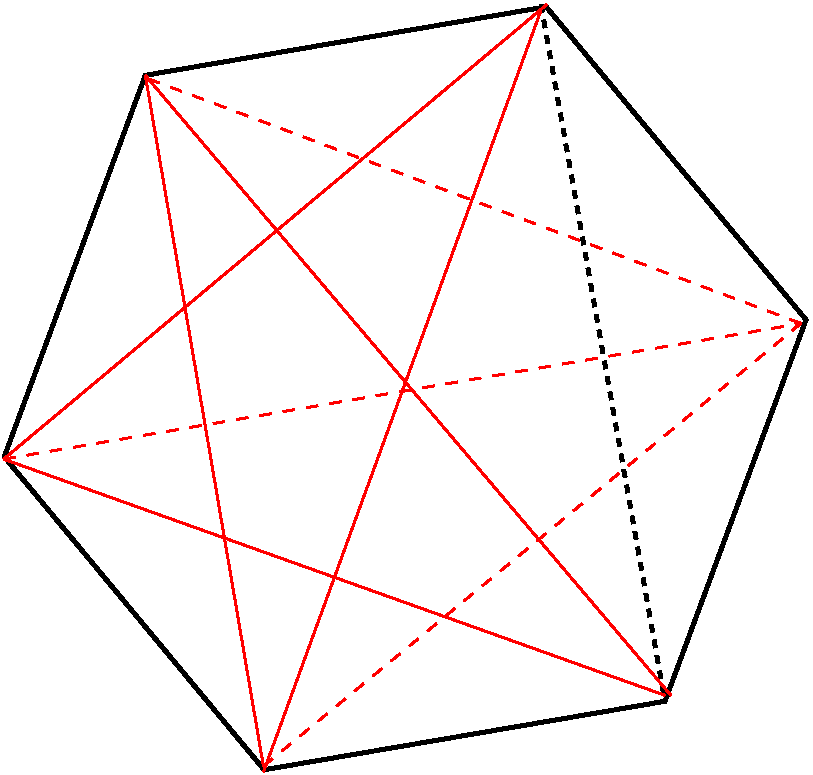
\includegraphics[width=6cm]{kuvat/kulmiot}
\end{center}

%(kuvio kun 5-kulmiosta täydennetään 6-kulmio)

Siten $(k + 1)$-sivuisen monikulmion lävistäjien lukumäärä on
\[
\frac{k (k - 3)}{2} +k-1=
\frac{k (k - 3)}{2} + \frac{2k - 2}{2}
=
\frac{k (k - 3)+2k-2}{2}=\frac{k^2-k-2}{2}.
\]
Polynomilla $k^2 - k - 2$ on nollakohdat $k = -1$ ja $k = 2$. Polynomi tekijöihinsä jaettuna
on $k^2 -k -2 = (k + 1)(k- 2)$. Siis $(k + 1)$-sivuisen monikulmion lävistäjien lukumäärä
\[
\frac{(k + 1)(k - 2)}{2}= \frac{(k + 1)((k + 1)-3)}{2}.
\]
Kaava pätee siis myös kuperille $(k + 1)$-sivuiselle monikulmiolle.

Induktioperiaatteen nojalla kaava on tosi, kun $n=3,4,5,\ldots$.
\qed

\newpage



\subsection*{Tehtäviä.}

\begin{enumerate}

\item Osoita induktiolla, että luku $n^2+n$ on jaollinen luvulla $2$, kun $n$ on luonnollinen luku.

\item Osoita induktiolla, että luku $n^3+2n$ on jaollinen luvulla $3$, kun $n$ on luonnollinen luku.

\item Osoita induktiolla, että $2^n > n$, kun $n$ on positiivinen kokonaisluku.

\item Osoita induktiolla, että $n^2 > 2n + 1$, kun $n$ on kokonaisluku ja $n \ge 3$.

\item Osoita, induktiolla, että luku $7^n + 5$ on jaollinen luvulla $6$, kun $n$ on positiivinen kokonaisluku.

\item Osoita induktiolla, että luku $10^n - 3^n$ on jaollinen luvulla $7$, kun $n$ on positiivinen kokonaisluku.

\item Osoita induktiolla, että luku $7^n - 6n + 8$ on jaollinen luvulla $9$, kun $n$ on positiivinen kokonaisluku.

\item Osoita induktiolla, että $n! > n^2$, kun $n$ on kokonaisluku ja $n \ge 4$. Merkintä $n!$ tarkoittaa luvun $n$ {\em kertomaa}. Se on tulo $n! = n \cdot (n-1) \cdot (n-2) \cdot \ldots \cdot 3 \cdot 2 \cdot 1$.

\item Olkoot $n$ positiivinen kokonaisluku ja $r$ reaaliluku, jolle pätee $r \neq 1$. Osoita induktiolla, että 
\[
1 + r + r^2 + r^3 + \ldots + r^{n-1} = \frac{1-r^n}{1-r}.
\]

\item Olkoon $n$ positiivinen kokonaisluku. Osoita induktiolla, että 
\[
1 \cdot 1! + 2 \cdot 2! + 3 \cdot 3! + \ldots + n \cdot n! = (n + 1)! - 1.
\]

\item 
Osoita induktiolla, että 
\[
\sum_{m=1}^n m^2= \frac{n(n+1)(2n+1)}{6}, \textrm{ kun } n=1,2,\ldots.
\]

\item
Osoita induktiolla, että $n$-alkioisessa joukossa on
\[
\frac{n(n-1)}{2}
\]
kahden alkion osajoukkoa, kun $n \ge 2$.

\item Todista kappaleessa 5.2 esiteltyjen kongruenssin laskusääntöjä koskevan lauseen kohta 4: Olkoot $a, b \in \Z$ ja $k,n \in \Z_+$ sekä $a \equiv b\ (\mod k)$. Tällöin $a^n \equiv b^n\ (\mod k)$.

\item Tarkastellaan kuviojonoa, joka muodostuu säännöllisen kuusikulmion muotoisista pistejoukoista. Jonon neljä ensimmäistä kuviota ovat seuraavat:

\begin{center}
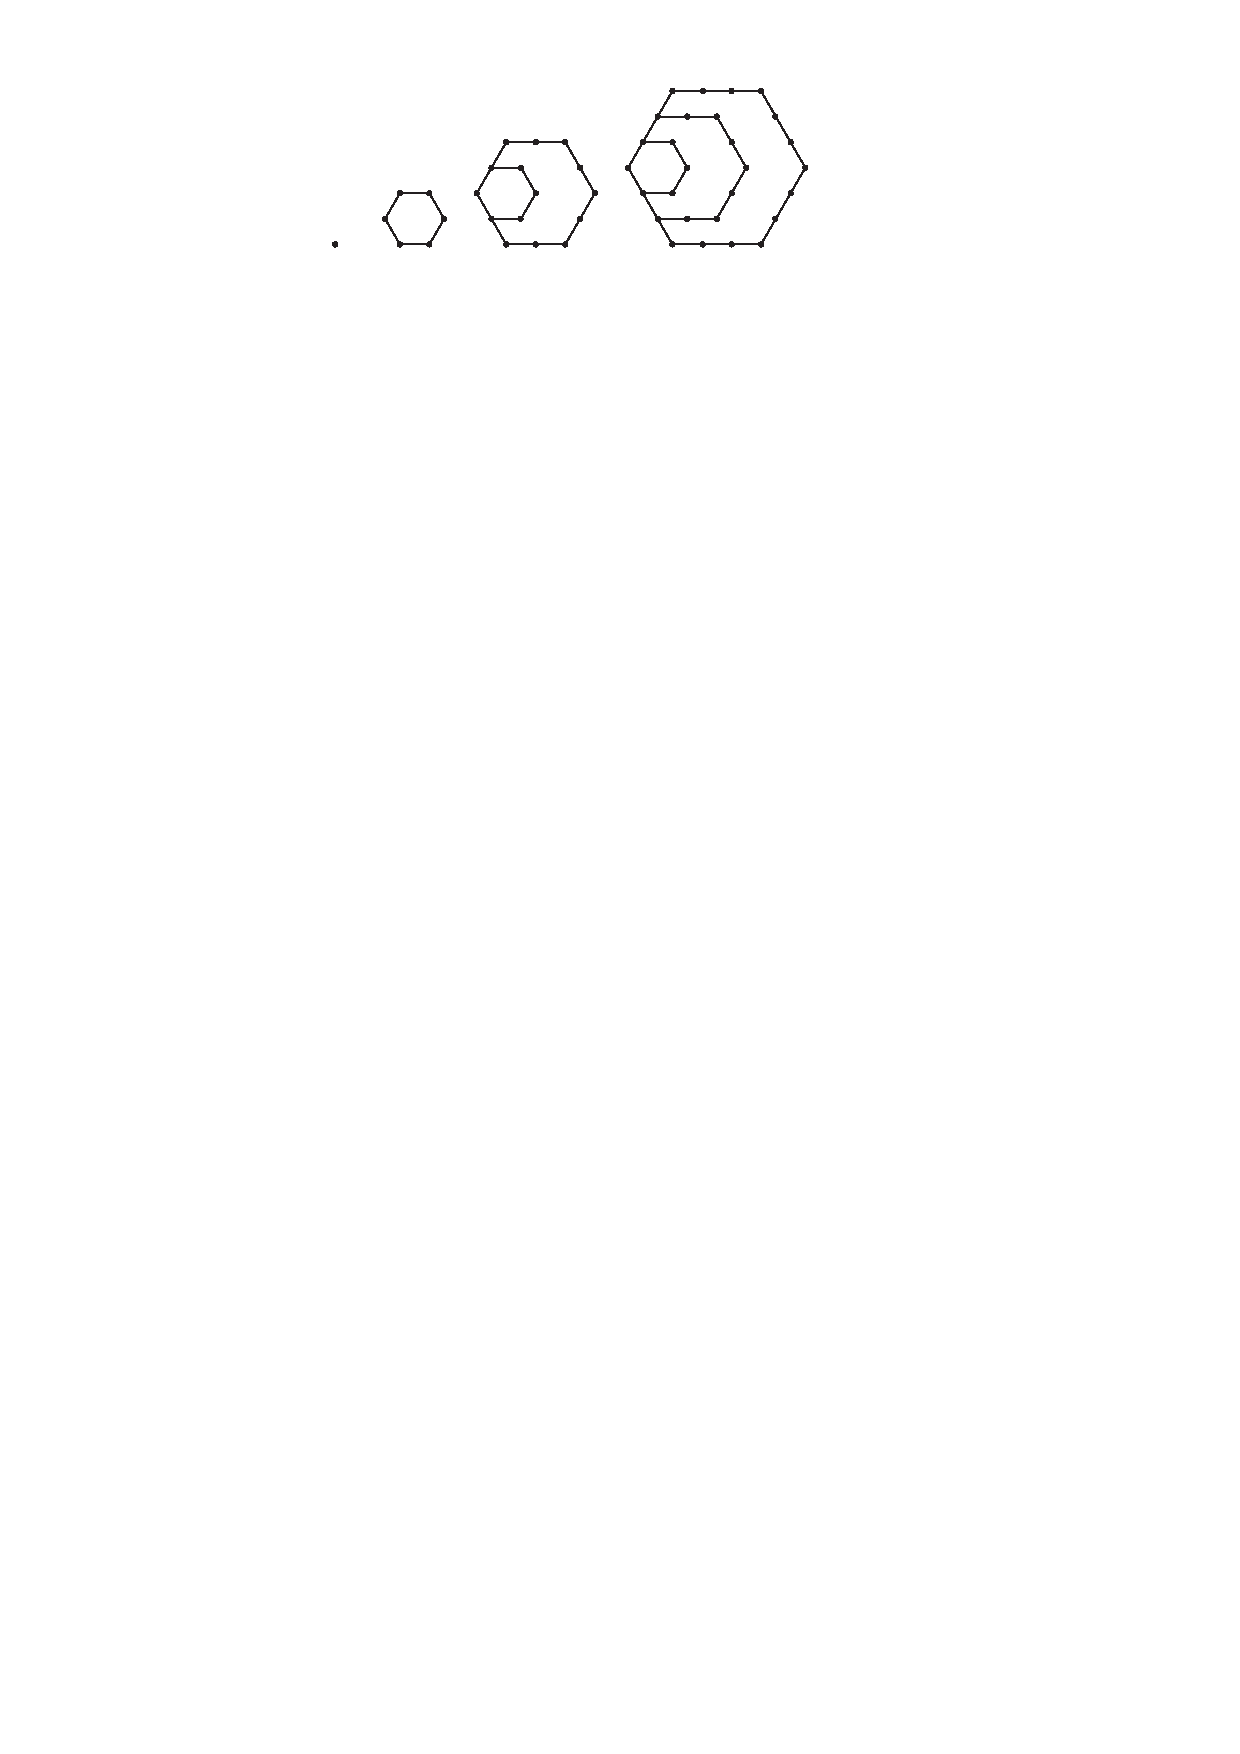
\includegraphics[width=10cm]{kuvat/Kappale5_4_kuusikulm_v2}
\end{center}


\begin{itemize}
\item[a)] Laske, kuinka monta pistettä on kuviojonon kussakin neljässä ensimmäisessä kuviossa.
\item[b)] Muodosta kaava, jolla voidaan laskea, kuinka monta pistettä on $n$. kuviossa. Tarpeen vaatiessa voit hyödyntää laskimesi polynomisovitustoimintoja.
\item[c)] Todista kaava induktiolla.
\end{itemize}

\end{enumerate}

{\bf Kotitehtäviä.}

\begin{enumerate}

\item Osoita induktiolla, että $n$ jakopisteellä jana voidaan jakaa enintään $n + 1$ janaksi.

\begin{center}
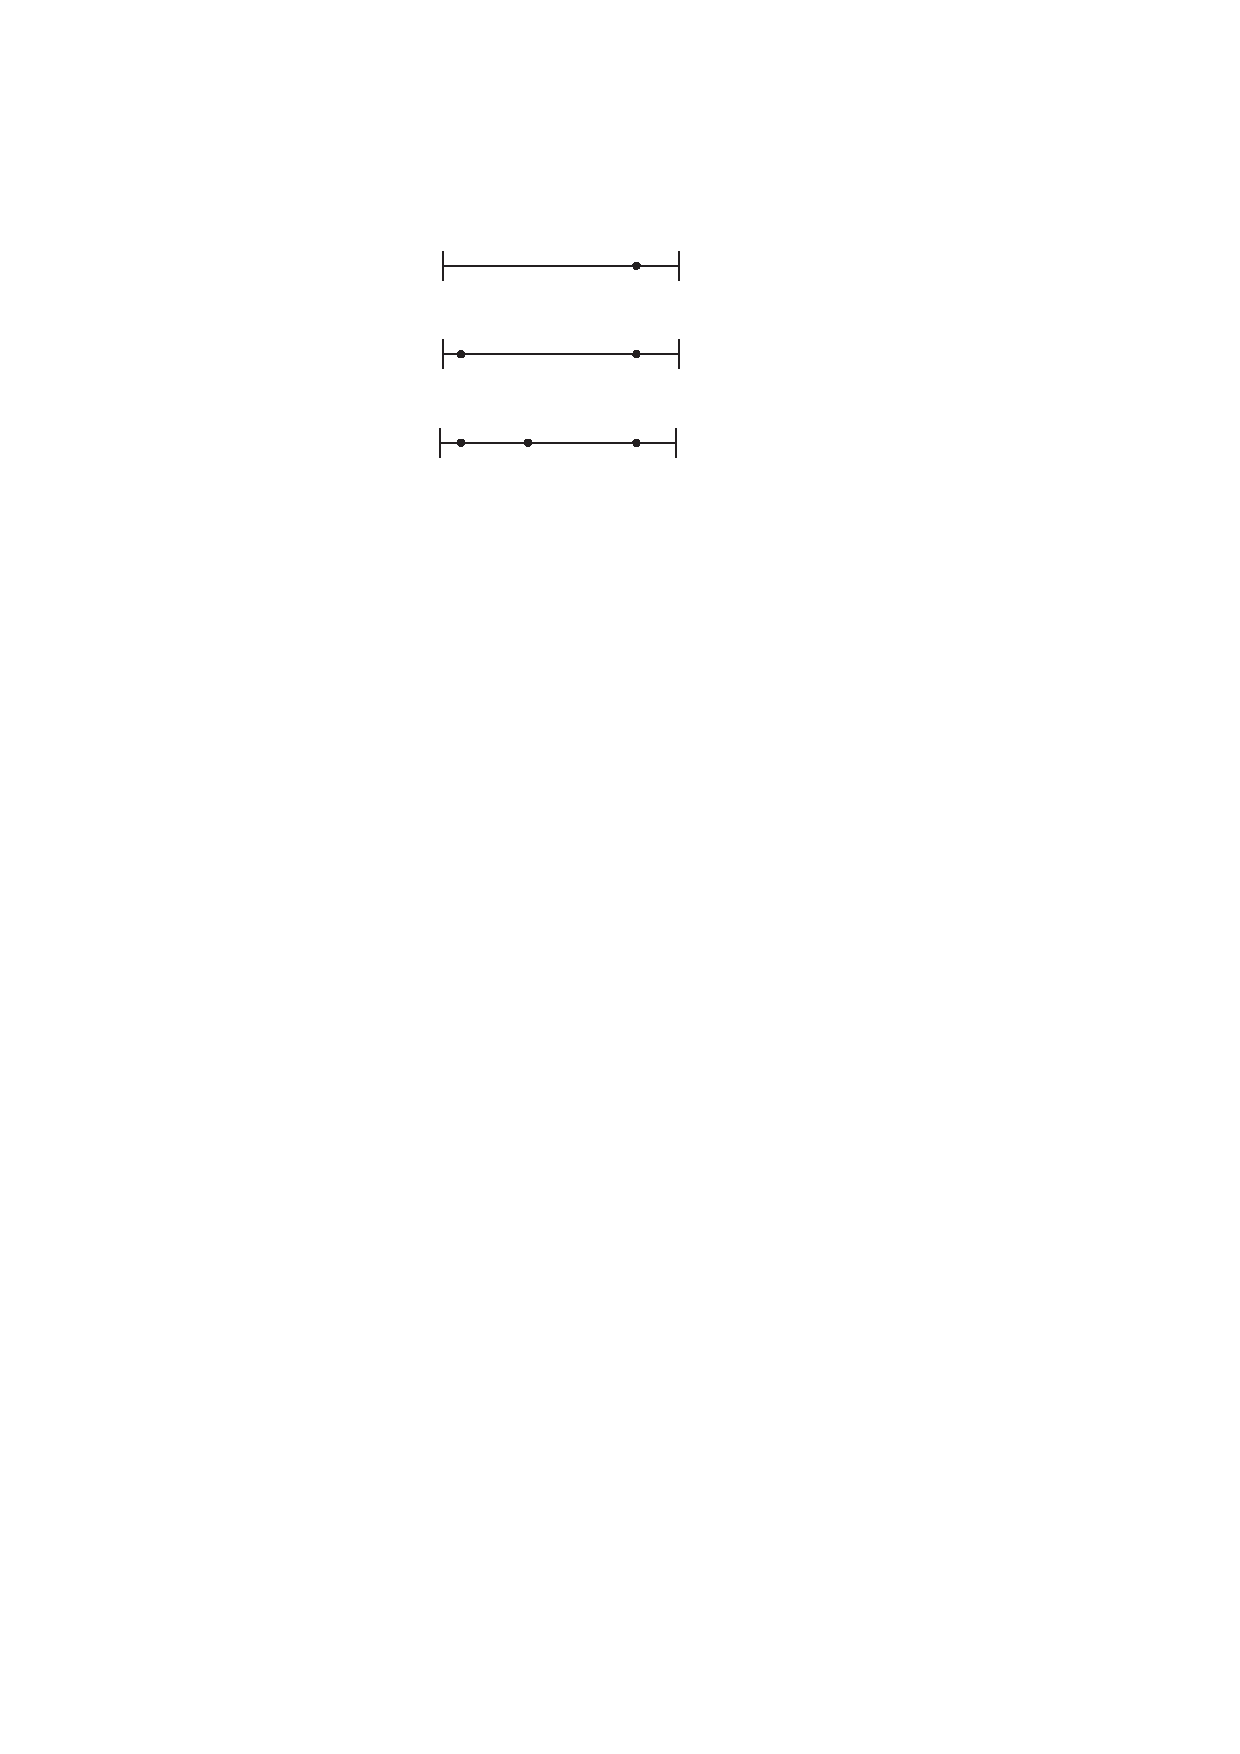
\includegraphics[width=6cm]{kuvat/Kappale5_4_janat_v2}
\end{center}

\item Osoita induktiolla, että luku $n^3 + 5n$ on jaollinen luvulla $6$, kun $n$ on luonnollinen luku.

\item Osoita, että $3^n > 2n$, kun $n$ on positiivinen kokonaisluku.

\item Osoita induktiolla, että $3^n < n!$, kun $n$ on kokonaisluku ja $n\ge 7$.

\item Osoita induktiolla, että luku $6^n - 1$ on jaollinen luvulla $5$, kun $n$ on positiivinen kokonaisluku.

\item Osoita induktiolla, että luku $8^n - 5^n$ on jaollinen luvulla $3$, kun $n$ on positiivinen kokonaisluku.

\item Osoita induktiolla, että luku $27^{2n} + 3 \cdot 13^{n}$ on jaollinen luvulla $4$, kun $n$ on positiivinen kokonaisluku.

\item 
Osoita induktiolla, että
\[
\sum_{m=1}^n m^3= \frac{n^2(n+1)^2}{4}, \textrm{ kun } n=1,2,\ldots.
\]

\item Osoita induktiolla, että $(1 + 2 + 3 +\ldots + n)^2 = 1^3 + 2^3 + 3^3 + \ldots + n^3$, kun $n$ on positiivinen kokonaisluku.

\item Tasoon piirretään $n$ suoraa ($n\ge 2$). Osoita, että suorilla voi olla korkeintaan $n(n - 1)/2$ leikkauspistettä.

\item Tarkastele seuraavia luvun $2$ peräkkäisistä potensseista muodostuvia summia:
\[
\begin{array}{rcl}
1 &=& 1\\
1 + 2 &=& 3\\
1 + 2 + 4 &=& 7\\
1 + 2 + 4 + 8 &=& 15\\
1 + 2 + 4 + 8 + 16 &=& 31\\
1 + 2 + 4 + 8 + 16 + 32 &=& 63\\
1 + 2 + 4 + 8 + 16 + 32 + 64 &=& 127.
\end{array}
\]
Muodosta kaava, jolla voidaan laskea summa $2^0 + 2^1 + 2^2 + \ldots + 2^n$, missä $n$ on luonnollinen luku. Todista kaava induktiolla.

\item Olkoot $n$ luonnollinen luku ja $x$ reaaliluku, jolle pätee $x > -1$. Osoita, että $(1 + x)^n \ge 1 + nx$. Kyseessä on niin sanottu {\em Bernoullin epäyhtälö}.

\item Olkoon $n$ positiivinen kokonaisluku. Todista, että
\[
\frac{1}{2}\le\frac{1}{n+1}+\frac{1}{n+2}+\ldots +\frac{1}{n+n} <1.
\]
[YO syksy 1971 tehtävä 7]


\item
Osoita, että kaikilla positiivisilla kokonaisluvuilla $n$ on
\[
1^2+3^2+5^2+\ldots+(2n-1)^2 = \frac{n(4n^2-1)}{3}. 
\]
[Ylioppilastehtävä K98 8b]

\item Tarkastellaan ruudukoista muodostuvaa kuviojonoa, jonka neljä ensimmäistä kuviota ovat seuraavat:

\begin{center}
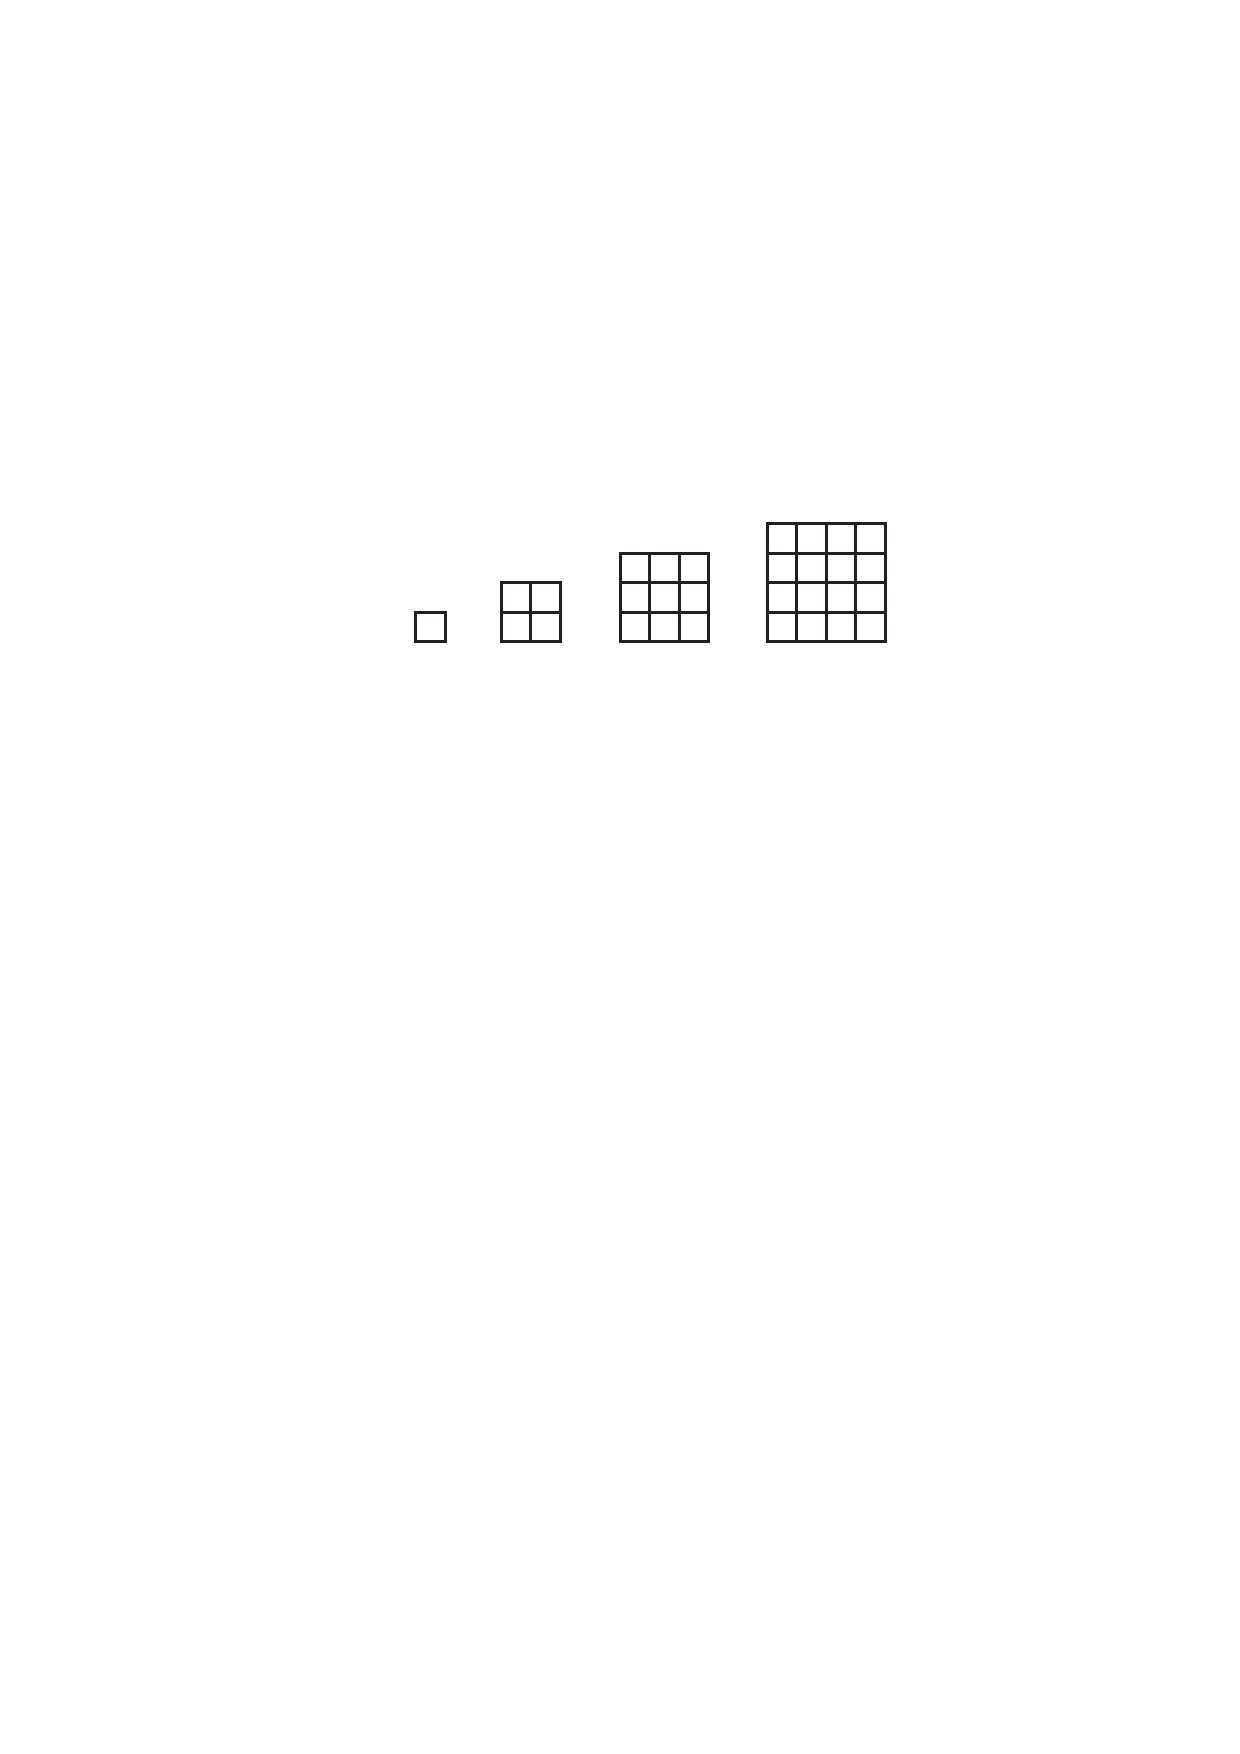
\includegraphics[width=10cm]{kuvat/Kappale5_4_ruudukko_v2}
\end{center}

\begin{itemize}
\item[a)] Laske, kuinka monta neliötä kaikkiaan on kuviojonon kussakin neljässä ensimmäisessä ruudukossa.
\item[b)] Muodosta kaava, jolla voidaan laskea, kuinka monta neliötä on $n$. ruudukossa. Tarpeen vaatiessa voit hyödyntää laskimesi polynomisovitustoimintoja.
\item[c)] Todista kaava induktiolla.
\end{itemize}

\item Eräs keino, jolla voi tarkastaa onko yhteenlasku oikein suoritettu, perustuu seuraavaan lauselmaan:

Jos useampien kokonaislukujen summa ja samoin näiden lukujen numerosummien summa jaetaan $9$:llä, niin tulevat jäännökset yhtä suuriksi. Todista tämä lauselma.
[YO 1895 tehtävä 2]


\end{enumerate}



\newpage

\section{Lukuteorian tuloksia}

Tässä luvussa käsitellään joitakin lukuteorian tunnetuimpia tuloksia ja niiden todistuksia.

\subsection{Suurin yhteinen tekijä ja Eukleideen algoritmi}
Seuraavaksi käsitellään kahden positiivisen kokonaisluvun yhteisiä tekijöitä ja esitetään käytännöllinen menetelmä {\em suurimman yhteisen tekijän} etsimiseksi.

\subsection*{Tutkimustehtävä}
\begin{enumerate}
\item Määritä lukujen $45$ ja $75$ kaikki positiiviset tekijät.
\item Mitkä ovat lukujen yhteiset positiiviset tekijät?
\item Mikä on lukujen suurin yhteinen tekijä?
\item Supista murtoluku $\frac{45}{75}$.
\end{enumerate}


{\bf Esimerkki 1.} Määritä lukujen $30$ ja $84$ kaikki positiiviset tekijät. Mitkä ovat niiden yhteiset positiiviset tekijät? Mikä on niiden suurin yhteinen tekijä?

{\bf Ratkaisu:} Luvun $30$ positiiviset tekijät ovat $1, 2, 3, 5, 6, 10, 15$ ja $30$. Luvun $84$ positiiviset tekijät ovat $1, 2, 3, 4, 6, 7, 12, 14, 21, 28, 42$ ja $84$.

Lukujen $30$ ja $84$ yhteiset positiiviset tekijät ovat $1, 2, 3$ ja $6$. Yhteisistä tekijöistä suurin on $6$.

{\bf Vastaus:} 
Yhteiset positiiviset tekijät ovat $1, 2, 3$ ja $6$. Suurin yhteinen tekijä on $6$.


\fbox{
\begin{minipage}{12cm}
{\large \bf Suurin yhteinen tekijä}

\medskip

%---
%{\bf Teorialaatikko [Suurin yhteinen tekijä]}
Olkoot $a$ ja $b$ positiivisia kokonaislukuja. Positiivista kokonaislukua $d$ sanotaan lukujen $a$ ja $b$  suurimmaksi yhteiseksi tekijäksi, jos seuraavat ehdot ovat voimassa:
\begin{enumerate}
\item Luku $d$ on lukujen $a$ ja $b$ tekijä, eli $d| a$ ja $d | b$. 
\item Luku $d$ on suurin lukujen $a$ ja $b$ tekijöistä.
\end{enumerate}
Lukujen $a$ ja $b$ suurinta yhteistä tekijää merkitään $\syt(a,b)$ tai joskus $\gcd(a,b)$. Lyhenne gcd tulee englanninkielisestä ilmaisusta {\em greatest common divisor}.
%---
\end{minipage}
}

Kahden luvun suurin yhteinen tekijä voidaan ainakin periaatteessa aina löytää luettelemalla näiden lukujen tekijät, etsimällä lukujen yhteiset tekijät ja valitsemalla lopuksi yhteisistä tekijöistä suurin. Tämä menettelytapa muuttuu kuitenkin hankalaksi suurten lukujen kohdalla, vaikka käytössä olisi tietokone.

Tehokkaan algoritmin suurimman yhteisen tekijän etsimiseksi esitti aleksandrialainen matemaatikko Eukleides (n. 300 eaa.) teoksessaan Stoikheia (Alkeet, latinaksi Elementa). Alkeet on yksi matematiikan historian tärkeimmistä teoksista, ja se säilyi käytetyimpänä geometrian oppikirjana aina 1800-luvulle saakka. Teoksessa esitettyä algoritmia kutsutaan {\em Eukleideen algoritmiksi}, ja se perustuu seuraavaan lemmaan:

%{\bf Lause (Jaollisuuden peruslause, s.108 / Pitkä matematiikka)}

{\bf Lemma.} Olkoot $a$ ja $b$ sellaisia positiivisia kokonaislukuja, että
\[
a=qb+r,
\]
missä $q$ sekä $r$ ovat kokonaislukuja ja $0<r<b$. Tällöin kokonaisluku $c$ on lukujen $a$ ja $b$ yhteinen tekijä, jos ja vain jos $c$ on lukujen $b$ ja $r$ yhteinen tekijä.

\proof
Oletetaan aluksi, että $c$ on jokin lukujen $a$ ja $b$ yhteinen tekijä. Osoitetaan, että se on myös lukujen $b$ ja $r$ yhteinen tekijä.

Kirjoitetaan $r=a-qb$. Luvun $c$ täytyy olla luvun $r$ tekijä, koska se on lukujen $a$ ja $b$ tekijä. Siten $c$ on lukujen $b$ ja $r$ yhteinen tekijä.

Oletetaan, että $c$ on jokin lukujen $b$ ja $r$ yhteinen tekijä. Koska $a=qb+r$, luvun $c$ täytyy olla myös luvun $a$ tekijä. Siten $c$ on lukujen $a$ ja $b$ yhteinen tekijä.

\qed

{\bf Seuraus.} Jos $a$ ja $b$ ovat positiivisia kokonaislukija ja $a=qb+r$, missä $q$ sekä $r$ ovat kokonaislukija ja $0<r<b$, niin $\syt(a,b)=\syt(b,r)$.

\proof
Lemman perusteella lukujen $a$ ja $b$ yhteiset tekijät ovat samat kuin lukujen $b$ ja $r$ yhteiset tekijät. Erityisesti siis lukujen $a$ ja $b$ suurimman yhteisen tekijän täytyy olla sama kuin lukujen $b$ ja $r$ suurimman yhteisen tekijän.
\qed

%{\bf ... täydennä}


Eukleideen algoritmin idea on seuraava: Lähdetään liikkeelle kahdesta positiivisesta kokonaisluvusta $a$ ja $b$, $a\ge b$, joiden yhteistä tekijää etsitään. Ensimmäinen askel on esittää luku $a$ luvun $b$ avulla jakoyhtälönä:
\[
a=q_1b + r_1, \qquad 0 \le r_1 < b.
\]

Jos jakojäännös $r_1=0$, niin $b|a$ ja $\syt(a,b)=b$. Jos $r_1\neq 0$, jaetaan $b$ luvulla $r_1$, jolloin saadaan esitys
\[
b= q_2r_1+r_2, \qquad 0 \le r_2 < r_1,
\]
missä $q_2$ on jakolaskun $b/r_1$ osamäärä ja $r_2$ jakojäännös.

Jos $r_2=0$, niin $r_1$ on suurin yhteinen tekijä ja voidaan lopettaa. Mikäli näin ei ole, jatketaan jakamalla luku $r_1$ luvulla $r_2$, jolloin saadaan
\[
r_1 = q_3r_2 + r_3, \qquad 0 \le r_3 < r_2.
\]

Näin jatkamalla päädytään lopulta jakolaskuun, joka menee tasan. Lukujen $a$ ja $b$ suurin yhteinen tekijä on viimeinen nollasta eroava jakojäännös. Koska algoritmissa esiintyy laskeva jono $b>r_1>r_2> \cdots \ge 0$, tarvitaan enintään $b$ askelta. Algoritmissa tarvittavat jakolaskut kannattaa yleensä tehdä laskimella.

{\bf Esimerkki 2.} Määritä $\syt(84, 30)$ Eukleideen
algoritmia käyttäen.

{\bf Ratkaisu:}

\begin{tabular}{lcl}
$84 = 2 \cdot 30 + 24$ & &
Jaetaan luku 84 luvulla 30 ja esitetään luku 84 luvun 30
\\
&& avulla. Jakojäännös ei ole nolla.\\
$30 = 1 \cdot 24 + 6$ & & Jaetaan luku 30 saadulla
jakojäännöksellä 24 ja \\
&& esitetään luku 30 luvun 24 avulla. Jakojäännös ei \\
&& ole nolla. \\
$24 = 4 \cdot 6$ & & Esitetään luku 24 jakojäännöksen 6
avulla. Nyt jako \\
&& menee tasan.
\end{tabular}

(Kuvioon tulee nuolet luvusta 30 lukuun 30 ja luvusta 24
lukuun 24, sekä luvusta 24
lukuun 24 ja luvusta 6 lukuun 6.)

Suurin yhteinen tekijä on viimeinen nollasta eroava
jakojäännös, $6$. Siis $\syt(84, 30) = 6$. Saatiin sama
tulos kuin esimerkissä 1.

{\bf Vastaus:} $\syt(84, 30) = 6$.

{\bf Esimerkki 3.} Määritä $\syt(16515,3951)$ Eukleideen
algoritmia käyttäen.

{\bf Ratkaisu:}
Eukleideen algoritmi johtaa yhtälöihin:
\[
16515 = 4 \cdot 3951 + 711,
\]
\[
3951 = 5 \cdot 711 + 396,
\]
\[
711 = 1 \cdot 396 + 315,
\]
\[
396 = 1 \cdot 315 + 81,
\]
\[
315 = 3 \cdot 81 + 72,
\]
\[
81 = 1 \cdot 72 + 9,
\]
\[
72 = 8 \cdot 9.
\]
Suurin yhteinen tekijä on viimeinen nollasta eroava
jakojäännös, siis tässä tapauksessa $9$. Siten
\[
\syt(16515,3951) = 9.
\]

{\bf Vastaus:} $\syt(16515, 3951) = 9$.

\newpage


\subsection*{Tehtäviä}

\begin{enumerate}

\item Määritä lukujen suurin yhteinen tekijä.
\begin{itemize}
\item[a)] $15$ ja $20$
\item[b)] $9$ ja $36$
\item[c)] $4$ ja $7$
\end{itemize}

\item Määritä Eukleideen algoritmia käyttäen
\begin{itemize}
\item[a)] $\syt(184,152)$
\item[b)] $\syt(227,143)$.
\end{itemize}

\item Määritä Eukleideen algoritmia käyttäen
\begin{itemize}
\item[a)] $\syt(272,1479)$
\item[b)] $\syt(4719,18207)$.
\end{itemize}

\item Esitä murtoluku  a) $\frac{143}{605}$  b) $\frac{5989}{30899}$  supistetussa muodossa. Vihje: Määritä osoittajan ja nimittäjän suurin yhteinen tekijä.

\item Osoita, että murtoluku $\frac{8788}{13475}$ ei supistu.

\item Leirille osallistui 780 tyttöä ja 612 poikaa. Osallistujat jaettiin keskenään yhtä suuriin ryhmiin siten, että kussakin ryhmässä oli vain tyttöjä tai poikia. Mikä oli suurin mahdollinen ryhmäkoko?

\item
Määritä lukujen $188\, 000\, 100$ ja $188$ suurin yhteinen tekijä.

\item Olkoon $a$ positiivinen kokonaisluku. Määritä
\begin{itemize}
\item[a)] $\syt(a,a)$
\item[b)] $\syt(a,1)$
\item[c)] $\syt(a^2,a)$
\item[d)] $\syt((a+1)!,a!)$.
\end{itemize}
Merkintä $a!$ tarkoittaa luvun $a$ {\em kertomaa}. Se on tulo $a! = a \cdot (a-1) \cdot (a-2) \cdot \ldots \cdot 3 \cdot 2 \cdot 1$.

\item Olkoon $n$ positiivinen kokonaisluku. Osoita Eukleideen algoritmia käyttäen, että $\syt(n+1,n)=1$.

\item Olkoon $n$ positiivinen kokonaisluku. Määritä lukujen $n^2 + 2n$ ja $n + 1$ suurin yhteinen tekijä.

\item Olkoon $n$ positiivinen kokonaisluku. Osoita, että $\syt(3^{n+1} + 10,3^n + 2)=1$.

\end{enumerate}


{\bf Kotitehtäviä}

\begin{enumerate}

\item Määritä lukujen suurin yhteinen tekijä.
\begin{itemize}
\item[a)] $63$ ja $7$
\item[b)] $64$ ja $33$
\item[c)] $45$ ja $60$
\end{itemize}

\item Määritä Eukleideen algoritmia käyttäen
\begin{itemize}
\item[a)] $\syt(657,306)$
\item[b)] $\syt(2197,4641)$
\item[c)] $\syt(15787,4111)$.
\end{itemize}

\item
Esitä murtoluku  a) $\frac{182}{299}$  b) $\frac{7697}{32041}$  supistetussa muodossa.

\item Leipomo suljettiin remontin ajaksi. Ennen sulkemista laskettiin, että leipomon varastossa oli 4896 vehnäsämpylää ja 1408 grahamsämpylää. Sämpylät pakattiin kuljetusta varten keskenään samankokoisiin pusseihin siten, että kuhunkin pussiin tuli vain vehnä- tai grahamsämpylöitä. Mikä oli suurin mahdollinen pussikoko? Oletetaan, että vehnäsämpylä oli samankokoinen kuin grahamsämpylä ja että yksikään pussi ei jäänyt vajaaksi.

\item Määritä lukujen $468\, 468\, 468\, 108$ ja $234$ suurin yhteinen tekijä.

\item Olkoot $a$, $b$ ja $c$ positiivisia kokonaislukuja. Lukujen $a$, $b$ ja $c$ suurin yhteinen tekijä eli $\syt(a,b,c)$ voidaan määrittää siten, että ensin määritetään kahden luvun suurin yhteinen tekijä ja sitten tämän ja kolmannen luvun suurin yhteinen tekijä. Määritä
\begin{itemize}
\item[a)] $\syt(15,30,40)$
\item[b)] $\syt(6,9,11)$
\item[c)] $\syt(171,456,665)$.
\end{itemize}

\item Olkoot $a$ ja $b$ positiivisia kokonaislukuja ja $\syt(a,b)=9$. Voiko tällöin yhtälö $a + b = 186$ olla tosi?

\item Olkoon $n$ positiivinen kokonaisluku. Tutki, mitä arvoja $\syt(n+4,n)$ voi saada.

\item Olkoon $n$ positiivinen kokonaisluku. Määritä lukujen $n^2 + 3n$ ja $n + 2$ suurin yhteinen tekijä.

\item Olkoot $a$ ja $b$ positiivisia kokonaislukuja. Osoita, että $\syt(a,b)$ on jaollinen kaikilla lukujen $a$ ja $b$ yhteisillä tekijöillä.

\end{enumerate}


\newpage

\subsection{Diofantoksen yhtälöt}
Noin vuoden 250 tienoilla elänyt Diofantos oli yksi viimeisistä antiikin Aleksandriassa vaikuttaneista suurista matemaatikoista. Aleksandrian suuruuden ajan oppineisuuden keskuksena katsotaan yleisesti päättyneen noin sata vuotta myöhemmin pakanaksi ja noidaksi syytetyn naismatemaatikko Hypatian murhaan vuonna 415. Vaikka Diofantos kirjoitti kreikaksi ja häntä usein kutsutaan kreikkalaiseksi matemaatikoksi, Diofantos oli todennäköisesti kreikkalaistunut babylonialainen. 

\subsection*{Tutkimustehtävä}
\begin{enumerate}
\item Missä sijaitsevat ne $xy$-tason pisteet, joiden koordinaatit toteuttavat yhtälön $x + 3y = 6$?
\item Etsitään seuraavaksi kokonaislukuratkaisuja kahden muuttujan yhtälölle $x + 3y = 6$. Määritä yhtälölle jokin kokonaislukuratkaisu.
\item Määritä yhtälölle vielä ainakin kolme muuta kokonaislukuratkaisua. Kuinka monta ratkaisua yhtälöllä on kaiken kaikkiaan?
\item Määritä kaikki yhtälön $x + 3y = 6$ kokonaislukuratkaisut.
\item Keksi vastaava kokonaislukukertoiminen kahden muuttujan yhtälö, jolla ei ole yhtään kokonaislukuratkaisua.
\end{enumerate}

{\bf Marginaaliin:}
Diofantoksesta ei tiedetä kovinkaan paljon, mutta hänen tarkka \hbox{elin}\-ikän\-sä tunnetaan kuitenkin hautakiveen ikuistetusta matemaattisesta ongelmasta: Diofantoksen poikavuodet kestivät $1/6$ hänen elämästään, parta alkoi kasvaa $1/12$ tämän jälkeen, $1/7$ kuluttua hän meni naimisiin ja hänen poikansa syntyi $5$ vuotta myöhemmin. Poika eli puolet siitä, mitä isänsä, ja isä kuoli neljä vuotta poikansa kuoleman jälkeen. Ongelma johtaa yhtälöön
\[
\frac{1}{6}x + \frac{1}{12} x + \frac{1}{7}x + 5 + \frac{1}{2}x+ 4=x,
\]
josta Diofantoksen elinvuodet voidaan ratkaista. Ratkaisu on $x=84$.

{\em Diofantoksen yhtälöiksi} kutsutaan muotoa
\[
ax + by = c
\]
olevia yhtälöitä, missä $x$ ja $y$ ovat kokonaislukuja. Yhtälössä esiintyvät vakiot $a,b$ ja $c$ ovat myös kokonaislukuja ja ainakin toinen luvuista $a,b$ on nollasta poikkeava. 
Tässä kurssissa käsitellään vain kyseistä muotoa olevia yhtälöitä, mutta nykyään matematiikassa sanotaan Diofantoksen yhtälöiksi myös muita yhtälöitä, joissa ratkaistavana on yksi tai useampi kokonaisluku. Diofantos ei itse tutkinut tällaisia yhtälöitä.

Diofantoksen yhtälöllä voi olla useita ratkaisuja tai ei yhtään ratkaisua. Esimerkiksi
yhtälölle
\[
3x + 6 y = 18
\]
voidaan löytää ainakin seuraavat ratkaisut:
\[
18 = 3\cdot 4 + 6\cdot 1 = 3\cdot (-6)+6\cdot 6 = 3\cdot10 + 6\cdot (-2).
\]
Toisaalta esimerkiksi yhtälöllä $2x+10 y =17$ ei ole ratkaisua.

Ratkaisujen etsimisessä on hyötyä tiedosta, että jos on annettu positiiviset kokonaisluvut $a$ ja $b$, niin on aina olemassa kokonaisluvut $x$ ja $y$ siten, että
%positiivisille kokonaisluvuille $a,b$ on aina olemassa kokonaisluvut $x$ ja $y$, joille
\[
\syt(a,b) = ax + by.
\]
Käytännössä kertoimien etsiminen ei ole vaikeaa, sillä siinä voidaan käyttää hyväksi Eukleideen algoritmia.
% Tästä esitysmuodosta ja Eukleideen algoritmista hyötyä Diofantoksen yhtälöiden ratkaisemisessa.

{\bf Esimerkki 1.} Ratkaise Diofantoksen yhtälö
$\syt(84,30) = 84x + 30y$.

{\bf Ratkaisu:} Lukujen $84$ ja $30$ suurin yhteinen tekijä
ratkaistiin edellisen kappaleen esimerkissä 2. Eukleideen
algoritmi johti yhtälöihin
\begin{eqnarray*}
84 &=& 2 \cdot 30 + 24,\\
30 &=& 1 \cdot 24 + 6,\\
24 &=& 4 \cdot 6,
\end{eqnarray*}
joten $\syt(84,30) = 6$. Ratkaistavana on siis yhtälö $6
= 84x + 30y$.

Pyritään nyt ilmaisemaan luku 6 lukujen 84 ja 30 avulla.
Kuljetaan Eukleideen algoritmia lopusta alkuun ja
ratkaistaan jakoyhtälöistä jakojäännökset. Viimeinen
nollasta eroava jakojäännös on $6$. Lausutaan se lukujen
$30$ ja $24$ avulla: $6 = 30 - 1 \cdot 24$. Saadussa
lausekkeessa luku $24$ on edellisen yhtälön jakojäännös,
joka puolestaan voidaan lausua lukujen $84$ ja $30$
avulla: $24 = 84 - 2 \cdot 30$. Yhdistämällä tulokset
saadaan luku $6$ ilmaistua lukujen $84$ ja $30$ avulla:
\[
6 = 30 - 1 \cdot 24 = 30 - 1 \cdot (84 - 2 \cdot 30) = 30
- 1 \cdot 84 + 2 \cdot 30 = -1 \cdot 84 + 3 \cdot 30.
\]
Siis $6 = 84 \cdot (-1) + 30 \cdot 3$, joten yhtälön $6=84x+30y$
ratkaisu on $x = -1$ ja $y = 3$.

{\bf Vastaus:} $x = -1$ ja $y = 3$.
 %Samat luvut kuin edellisen kappaleen esimerkissä 2.

Diofantoksen yhtälöitä voidaan usein ratkaista esimerkiksi tietokoneella, mutta se onnistuu myös seuraavaa tulosta käyttämällä.

{\bf Lause.} Diofantoksen yhtälöllä
\[
a x + b y = c
\]
on ratkaisu, jos ja vain jos $d|c$, kun $d=\syt(a,b)$.

\proof
%{\bf Mieti todistuksen muotoilua, vars. jos ja vain jos.}
%Jaa kahteen osaan, ensin toiseen ja sitten toiseen suuntaan. Oletukset eksplisiittisesti.

Osoitetaan aluksi epäsuoraa todistusta käyttämällä, että ratkaisun olemassaolosta seuraa $d|c$. Tehdään vastaoletus, että $d \nmid c$. Tällöin yhtälöllä ei voi olla ratkaisua, koska $d|a$ ja $d|b$, joten $d$ jakaa yhtälön vasemman puolen mutta ei oikeaa puolta.

On vielä osoitettava ekvivalenssiväitteen toinen suunta: Jos $d|c$, niin kyseisellä Diofantoksen yhtälöllä on ratkaisu. Jos $d|c$, niin $c=dt$ jollakin kokonaisluvulla $t$. Aikaisemmin todettiin, että lukujen $a$ ja $b$ suurin yhteinen tekijä voidaan kirjoittaa muodossa
\[
d=\syt(a,b)=a x_1 + b y_1
\]
joillekin luvuille $x_1$ ja $y_1$. Koska
\[
c = dt = (ax_1 + by_1)t = a(tx_1)+ b(ty_1),
\]
saadaan pari $x=tx_1$ ja $y=ty_1$, joka toteuttaa alkuperäisen yhtälön.
\qed

{\bf Lause.}
Jos
\[
a x + b y = c
\]
on ratkeava Diofantoksen yhtälö, sen yksi ratkaisu on $x=tx_1$ ja $y=ty_1$, missä kertoimet $x_1$ ja $y_1$ määräytyvät yhtälöstä
\[
d=\syt(a,b)=a x_1 + b y_1 \textrm{ ja } t=c/d.
\]

\proof
Edellisen lauseen nojalla Diofantoksen yhtälöllä
\[
d= a x + b y,
\]
missä $d=\syt(a,b)$, on ratkaisu. Merkitään jotakin kyseisen yhtälön ratkaisua $x_1,y_1$.

On osoitettava, että tämän ratkaisun avulla voidaan löytää haluttua muotoa oleva ratkaisu alkuperäiselle yhtälölle
\[
a x + b y = c.
\]
Edellisen lauseen perusteella Diofantoksen yhtälöllä on ratkaisu, jos ja vain jos $d|c$. Siten $t=c/d$ on kokonaisluku.

Kerrotaan yhtälön
\[
d= a x_1 + b y_1
\]
molemmat puolet luvulla $t=c/d$. Tällöin saadaan
\[
c=td=t(a x_1 + b y_1) = a(tx_1)+ b(ty_1).
\]
Tämä osoittaa, että $x=tx_1$ ja $y=ty_1$ on alkuperäisen Diofantoksen yhtälön ratkaisu.
\qed

Itse asiassa jos $x_0$ ja $y_0$ ovat yhtälön $ax + by = c$ jokin ratkaisu, niin sen kaikki ratkaisut saadaan kaavoista
\[
x= x_0 + n\frac{b}{d}, \textrm{ ja } y=y_0 - n\frac{a}{d}, \textrm{ missä } \qquad n\in\mathbb{Z} \textrm{ ja } d=\syt(a,b).
\]
Erityisesti siis jokaisella ratkeavalla Diofantoksen yhtälöllä on äärettömän monta ratkaisua. Ratkaisussa esiintyvät kertoimet saattavat kuitenkin olla negatiivisia lukuja.

{\bf Esimerkki 2.} Määritä Diofantoksen yhtälön
\[
172x + 20y = 1000
\]
jokin ratkaisu.

{\bf Ratkaisu:} Tutkitaan ensin, onko Diofantoksen yhtälöllä $172x + 20y = 1000$ ratkaisua. Määritetään $\syt(172,20)$ Eukleideen algoritmia käyttäen:
\[
172 = 8 \cdot 20 +12,
\]
\[
20 = 1\cdot 12 + 8,
\]
\[
12 = 1 \cdot 8 +4,
\]
\[
8=2\cdot 4.
\]
Siten $\syt(172,20)=4$. Koska $4|1000$, Diofantoksen yhtälöllä on ratkaisu.

Ratkaisun löytämiseksi täytyy esittää luku $4$ lukujen $172$ ja $20$ avulla muodossa 
\[
4=172\cdot x_1 + 20 \cdot y_1.
\]
Soveltamalla Eukleideen algoritmin askelia käänteisessä järjestyksessä saadaan
\begin{eqnarray*}
4 &=& 12 - 8\\
  &=& 12-(20-12) \\
  &=& 2\cdot 12-20 \\
  &=& 2 \cdot (172-8\cdot 20)-20 \\
  &=& 2\cdot 172 +(-17) \cdot 20.
\end{eqnarray*}
Kertomalla tämä lauseke luvulla $1000/4=250$ saadaan viimein
\begin{eqnarray*}
1000 = 250\cdot 4 &=& 250 \cdot (2\cdot 172 +(-17) \cdot 20) \\
 &=& 500\cdot 172 + (-4250) \cdot 20.
\end{eqnarray*}
Siten yhtälön $172x + 20y = 1000$ ratkaisu on $x=500$ ja $y=-4250$.

{\bf Vastaus:} $x=500$ ja $y=-4250$


{\bf Esimerkki 3.}
Määritä Diofantoksen yhtälön $172x + 20y = 1000$ kaikki
ratkaisut. Mitkä niistä toteuttavat ehdon $|x|+|y|\le
50$?

{\bf Ratkaisu:}
Diofantoksen yhtälön $ax+by=c$ kaikki ratkaisut saadaan
kaavoista
\[
x=x_0+n\frac{b}{d}\textrm{ ja }y=y_0-n\frac{a}{d},
\]
missä $x_0$ ja $y_0$ ovat yhtälön jokin ratkaisu,
$d=\syt(a,b)$ ja $n$ on mikä tahansa
kokonaisluku. Diofantoksen yhtälössä $172x+20y=1000$ on
$a=172$, $b=20$, ja edellisen
esimerkin nojalla $x_0=500$, $y_0=-4250$ ja $d=4$.
Sijoittamalla kaavoihin saadaan
yhtälön $172x+20y=1000$ ratkaisuiksi
\[
x=500+n\frac{20}{4}\textrm{ ja }y=-4250-n\frac{172}{4}
\]
eli $x=500+5n$ ja $y=-4250-43n$, $n\in\Z$.

Jotta ehto $|x| +|y|\le 50$ toteutuisi, pitää muuttujien
$x$ ja $y$ olla itseisarvoiltaan pieniä. Tutkitaan
yhtälöitä $x = 500 + 5n = 0$ ja $y = -4250 - 43n = 0$ ja
ratkaistaan kummastakin parametri $n$.
\begin{eqnarray*}
500 + 5n &=& 0\\
5n &=& -500\\
n &=& -100\\
-4250 - 43n &=& 0\\
-43n &=& 4250\\
n &\approx&-98,8
\end{eqnarray*}
Osoittautuu siis, että molempien yhtälöiden mukaan $n$
on lähellä arvoa $-100$ tai $-99$. Taulukoidaan myös
muutamia muita näitä arvoja lähellä olevia parametrin $n$
arvoja ja tutkitaan kussakin tapauksessa, toteutuuko ehto
$|x| + |y| \le 50$.

\begin{center}
\begin{tabular}{|c|c|c|c|}
\hline
$n$ & $x$ & $y$ & $|x|+|y|$ \\

\hline
$-97$&$15$&$-79$&$94$\\
\hline
$-98$&$10$&$-36$&$46$\\
\hline
$-99$&$5$&$7$&$12$\\
\hline
$-100$&$0$&$50$&$50$\\
\hline
$-101$&$-5$&$93$&$98$\\
\hline
$-102$&$-10$&$136$&$146$\\
\hline
\end{tabular}
\end{center}

Taulukosta nähdään, että $|x|+|y| \le 50$, kun $x = 10$
ja $y = -36$, kun $x = 5$ ja $y = 7$ tai kun $x = 0$ ja
$y = 50$. Muita ratkaisuja ei ole, sillä kun $n$ pienenee
tai suurenee taulukon arvoista, niin sekä $|x|$ että $|
y|$ suurenevat.

{\bf Vastaus:} Kaikki ratkaisut ovat  $x=500+5n$ ja $y=-4250-43n$, $n\in\Z$. Näistä ehdon $|x|+|y|\le 50$ toteuttavat ratkaisut $x = 10$ ja $y = -36$, $x = 5$ ja $y = 7$ sekä $x = 0$ ja $y = 50$.

{\bf Esimerkki 4.} (Kexleruksen viiniongelma)
(Lisämateriaalia)
Suomen ensimmäinen matematiikan professori, Turun
akatemiassa vaikuttanut Simon Kexlerus (1602--1669) jätti
jälkeensä seuraavan ongelman.

\begin{center}
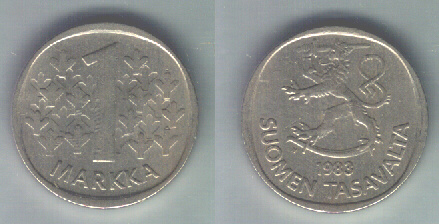
\includegraphics[width=4cm]{kuvat/wikimarkka.jpg} % /NVI

Markan kolikko vuodelta 1983.
\end{center}

Sinulla on viinejä, jotka maksavat $3$, $5$, $8$ ja $10$
markkaa pullolta. Ota yhteensä kymmenen täyttä pulloa ja
tee niistä sekoitus, joka maksaa $6$ markkaa pullolta.
Kuinka monta pulloa kutakin viinilajia on otettava?

{\bf Ratkaisu:} Merkitään tarvittavien pullojen määrää
$a,b,c$ ja $d$. Ongelma johtaa kahteen Diofantoksen
yhtälöön,
\[
a+b+c+d = 10
\]
ja
\[
3a+5b+8c+10d = 60.
\]
Selvästi tehtävän ratkaisut ovat kokonaislukuja välillä
$0,\ldots,10$. Tehtävä ei ole aikaisemmin esitettyä
muotoa. Siitä kuitenkin saadaan sellainen, jos oletetaan,
että käytetään vain kahta eri viiniä. Toisin sanoen,
asetetaan kaksi kertoimista $a,b,c,d$ nollaksi.

Kahden ensimmäisen viinin hinta on tavoitehintaa
alhaisempi ja kahden jälkimmäisen vastaavasti
tavoitehintaa korkeampi. Siksi ongelma voi ratketa kahta
viiniä käyttämällä vain, jos toinen valitaan seokseen
kahdesta edullisemmasta ja toinen kahdesta kalliimmasta
viinistä. Kokeillaan aluksi kertoimia $a=c=0$. Nyt
saadaan
\[
5b + 10d = 60.
\]
Koska $\syt(5,10)=5$ ja $5|60$, ratkaisu on olemassa.
Esitetään aluksi luku $5$ lukujen $10$ ja $5$ avulla:
\[
5 = -1 \cdot 5 + 1\cdot 10.
\]
Kertomalla luvulla $12$ saadaan
\[
60 = -12\cdot 5 + 12\cdot 10,
\]
joten yhtälöllä $5b+10d=60$ on ratkaisu $b=-12$ ja $d=12$. Tätä ratkaisua ei kuitenkaan voida hyväksyä, koska siinä esiintyy negatiivinen kerroin, $-12$, eikä se myöskään toteuta toista vaadittua yhtälöä, $b+d=10$.

Yhtälöllä on kuitenkin muitakin ratkaisuja. Ne saadaan
kaavoista
\[
b= -12 + (10/5)n, \qquad d=12 - (5/5)n,
\]
eli
\[
b= -12 + 2n, \qquad d=12 - n,
\]
missä $n$ on mikä tahansa kokonaisluku. Sijoittamalla
yhtälöön $b+d=10$ saadaan
\[
-12 + 2n + 12 - n = 10,
\]
eli $n=10$. Ratkaisu on siis $b=-12+2 \cdot 10=8$ ja
$d=12-10=2$.

{\bf Vastaus:} On otettava esimerkiksi $8$ pulloa $5$
markan viiniä ja $2$ pulloa $10$ markan viiniä.

Esimerkiksi tietokonetta käyttämällä voidaan löytää
ongelman kaikki ratkaisut. Niitä on yhteensä seitsemän.
Ei ole tiedossa, miten Kexlerus itse ratkaisi ongelmansa.

\newpage


\subsection*{Tehtäviä}

\begin{enumerate}

\item Tutki, onko Diofantoksen yhtälöllä ratkaisua.
\begin{itemize}
\item[(a)] $7x + 5y = 3$
\item[(b)] $5x + 85y = 42$
\item[(c)] $6x + 51y = 100$
\end{itemize}

\item Leirille osallistui $364$ nuorta. Oliko mahdollista majoittaa osallistujat $24$ ja $16$ hengen parakkeihin siten, että yksikään parakki ei jäänyt vajaaksi?

\item Määritä Diofantoksen yhtälön jokin ratkaisu.
\begin{itemize}
\item[(a)] $14x + 49y = \syt(14,49)$
\item[(b)] $56x + 72y = \syt(56,72)$
\end{itemize}

\item Määritä Diofantoksen yhtälön jokin ratkaisu.
\begin{itemize}
\item[(a)] $56x + 72y = 40$
\item[(b)] $24x + 138y = -24$
\end{itemize}

\item Tutki, onko suoralla
\begin{itemize}
\item[(a)] $26x + 91y + 10 = 0$
\item[(b)] $529x + 621y - 92 = 0$
\end{itemize}
pisteitä, joiden molemmat koordinaatit ovat kokonaislukuja.

\item Määritä Diofantoksen yhtälön kaikki ratkaisut.
\begin{itemize}
\item[(a)] $2x + 3y = 1$
\item[(b)] $2x + 3y = 7$
\end{itemize}

\item Määritä Diofantoksen yhtälön $45x + 21y = -6$ kaikki ratkaisut.

\item Määritä Diofantoksen yhtälön $13\, 509x + 10\, 203y = 228$ kaikki ratkaisut.

\item Keksi Diofantoksen yhtälö, jolla a) ei ole ratkaisua b) on äärettömän monta ratkaisua.

\item Määritä Diofantoksen yhtälön $63x + 279y = 450$ kaikki ratkaisut. Mitkä niistä toteuttavat ehdon $|x| + |y| < 25$?

\item Käytettävissä on $8$ gramman ja $12$ gramman punnuksia. Kuinka monta kummankinlaista punnusta tarvitaan, jotta punnusten kokonaismassaksi tulisi $100$ grammaa? Selvitä kaikki vaihtoehdot. 

\item Ruhtinas jakoi $63$ yhtä suurta kekoa hedelmiä sekä $7$ erillistä hedelmää tasan $23$ matkalaiselle. Kuinka monta hedelmää kussakin keossa oli? Vihje: Tutki yhtälöä $63x + 7 = 23y$. (Mahavira, v. 850)

\item Olkoot $a$, $b$, $c$ ja $d$ positiivisia kokonaislukuja. Osoita, että yhtälöllä $ax+by+cz=d$ on kokonaislukuratkaisu, jos ja vain jos luku $d$ on jaollinen lukujen $a,b$ ja $c$ suurimmalla yhteisellä tekijällä. 

\end{enumerate}

{\bf Kotitehtäviä}

\begin{enumerate}

\item Tutki, onko Diofantoksen yhtälöllä ratkaisua.
\begin{itemize}
\item[(a)] $9x + 6y = 72$
\item[(b)] $12x + 10y = 323$
\item[(c)] $14x + 35y = -91$
\end{itemize}

\item Emilia sai valmistujaislahjaksi $200$ euron lahjakortin erääseen keramiikkapajaan. Hän osti pajasta $27$ euron hintaisia kynttilänjalkoja ja $15$ euron hintaisia jälkiruokalautasia. Hän maksoi ostoksensa lahjakortilla ja sai rahaa takaisin $12$ euroa. Laskiko myyjä oikein?

\item Määritä Diofantoksen yhtälön jokin ratkaisu.
\begin{itemize}
\item[(a)] $59x + 12y = \syt(59,12)$
\item[(b)] $119x + 272y = \syt(119,272)$
\end{itemize}

\item Määritä Diofantoksen yhtälön jokin ratkaisu.
\begin{itemize}
\item[(a)] $36x + 16y = 28$
\item[(b)] $221x + 35y = 2$
\end{itemize}

\item Määritä Diofantoksen yhtälön kaikki ratkaisut.
\begin{itemize}
\item[(a)] $2x + 6y = 2$
\item[(b)] $2x + 6y = -10$
\end{itemize}

\item Määritä Diofantoksen yhtälön $35x + 84y = 14$ kaikki ratkaisut.

\item Määritä Diofantoksen yhtälön $11\, 925x + 3\, 843y = -117$ kaikki ratkaisut.

\item Määritä Diofantoksen yhtälön $168x + 204y = 24$ kaikki ratkaisut. Mille ratkaisuille pätee $-50 \le x \le 0$ ja $y > 10$?

\item  Esitä luku $100$ kahden positiivisen kokonaisluvun summana niin, että toinen luvuista on jaollinen luvulla $7$ ja toinen luvulla $11$. (Euler, v. 1770)

\item Yhtiön kauppavoitto 150 mk on jaettava tasan osakkaille. Jos osakkaita olisi ollut 5 enemmän, olisi jokainen saanut 5 mk vähemmän. Montako osakasta oli yhtiössä? 
[YO 1874 tehtävä 6]

\item Sata lyhdettä viljaa jaetaan sadalle henkilölle niin, että kukin mies saa $3$ lyhdettä, nainen $2$ lyhdettä ja lapsi puoli lyhdettä. Kuinka monta miestä, naista ja lasta on? (Alcuin Yorkilainen, v. 775)

\item (Lisämateriaalia.) Osoita suoralla sijoituksella, että $a=2$, $b=4$, $c=3$ ja $d=1$ on yksi Kexleruksen viiniongelman ratkaisuista.

\item (Lisämateriaalia.) Ratkaise Kexleruksen viiniongelma, kun asetetaan $b=0$ ja $d=0$.

\item (Lisämateriaalia.) Osoita, että Kexleruksen viiniongelmalla ei ole ratkaisuja, jos asetetaan $a=0$ ja $d=0$.

\end{enumerate}


\newpage


\subsection{Alkuluvut ja aritmetiikan peruslause}

\subsection*{Tutkimustehtävä}
\begin{enumerate}
\item Millä positiivisilla kokonaisluvuilla luku $60$ on jaollinen?
\item Millä positiivisilla kokonaisluvuilla luku $29$ on jaollinen?
\item Esitä luku $60$ mahdollisimman pienten positiivisten kokonaislukujen tulona.
\end{enumerate}

{\em Alkuluvuksi} sanotaan luonnollista lukua $p\ge 2$, joka ei ole jaollinen muilla positiivisilla kokonaisluvuilla kuin itsellään sekä luvulla $1$. Esimerkiksi luku $13$ on alkuluku. Luku $14$ ei ole alkuluku, koska se on jaollinen myös luvuilla $2$ ja $7$.


{\bf Esimerkki 1.} Tutki, onko luku a) $23$, b) $357$ alkuluku.

{\bf Ratkaisu:}

a) Luku $23$ ei ole jaollinen luvulla $2$, sillä se ei ole
parillinen. Luku $23$ ei ole jaollinen luvulla $3$, sillä
\[
\frac{23}{3}= 7\frac{2}{3},
\]
joka ei ole kokonaisluku. Luku $23$ ei ole jaollinen luvulla $4$
eikä millään muullakaan parillisella luvulla, sillä se ei ole
jaollinen luvulla $2$. Luku $23$ ei ole
jaollinen luvulla $5$, sillä se ei pääty numeroon $0$ tai $5$.
Luku $23$ ei ole jaollinen luvulla $7$, sillä
\[
\frac{23}{7} = 3\frac{2}{7}.
\]
Luku $23$ ei ole jaollinen luvulla $9$, sillä se ei ole jaollinen
luvulla $3$. Luku $23$ ei ole jaollinen luvulla $11$, sillä
\[
\frac{23}{11} = 2\frac{1}{11}.
\]
Seuraava kokeiltava luku olisi $13$. Se on kuitenkin jo liian
suuri, sillä se on yli puolet luvusta $23$. Osoittautuu, että
luku $23$ on jaollinen ainoastaan itsellään ja luvulla $1$. Se on
siis alkuluku.

b) Luku $357$ ei ole jaollinen luvulla $2$, sillä se ei ole
parillinen. Se ei siis myöskään ole jaollinen millään muulla
parillisella luvulla. Koska $357 = 119 \cdot 3$, niin luku $357$
on jaollinen luvuilla $3$ ja $119$. Jaollisuus luvulla $3$
nähdään myös siitä, että luvun $357$ numeroiden summa $3 + 5 + 7
= 15$ on jaollinen luvulla $3$. Luku $357$ ei ole alkuluku.

{\bf Vastaus:} a) On. b) Ei ole.


Alkulukuja voidaan etsiä helpommin esimerkiksi yksinkertaisella algoritmilla, joka tunnetaan {\em Eratostheneen seulana}. Eratosthenes oli kreikkalainen matemaatikko, filosofi, runoilija, tähtitieteilijä ja historioitsija. Bysanttilaisten historioitsijoiden mukaan hän syntyi vuonna 276 eaa. nykyisessä Libyassa ja kuoli 81-vuotiaana vuonna 195 eaa. Eratosthenes vaikutti tuon ajan sivistyksen keskuksessa Aleksandriassa. Hänen kuuluisin keksintönsä lienee menetelmä maapallon ympärysmitan laskemiseksi. %Itse hän kuvaili itseään viisauden ystäväksi.

Algoritmin idea on seuraava. Halutaan löytää alkuluvut välillä $2,\ldots,n$.
\begin{enumerate}
\item Tehdään aluksi lista tutkittavista luvuista. 
\item Listan ensimmäinen luku $2$ on alkuluku. Aluksi poistetaan listasta kaikki lukua $2$ suuremmat luvut, jotka ovat jaollisia luvulla $2$.
\item Edetään seuraavaan listassa jäljellä olevaan lukuun $k$. Se ei ole jaollinen millään itseään pienemmällä alkuluvulla, joten sekin on alkuluku.
\item Poistetaan listasta kaikki lukua $k$ suuremmat luvut, jotka ovat jaollisia luvulla $k$.
\item Toistetaan vaiheita (3) ja (4) niin kauan, kun luku $k \le \sqrt{n}$. 
\end{enumerate}

Nyt listassa on jäljellä vain alkulukuja. Tämä voidaan nähdä seuraavasti: Olkoon
 välillä $]\sqrt{n}, n]$ jokin luku $z$, joka ei ole alkuluku. Tällöin voidaan
kirjoittaa $z = qm$, missä $q$ ja $m$ ovat positiivisia kokonaislukuja. Nyt pätee
 $q \le \sqrt{n}$ tai $m\le \sqrt{n}$, sillä jos $q >\sqrt{n}$ ja $m>\sqrt{n}$, 
niin $z=qm>\sqrt{n}\cdot \sqrt{n}=n$, mikä ei ole mahdollista. Koska $q\le \sqrt
{n}$ tai $m\le \sqrt{n}$, niin $z$ ei enää voi olla mukana listassa. Välillä $]\sqrt{n}, n]$ ei siis enää ole muita kuin alkulukuja.

Eratostheneen seula on käyttö\-kelpoinen etsittäessä suhteellisen pieniä alkulukuja. Suurempien alkulukujen etsimiseen on kehitetty monenlaisia matemaattisia algoritmeja. Suurten alkulukujen löytäminen on joskus tarpeellista etenkin lukuteoriaan pohjaavia salakirjoitusmenetelmiä käytettäessä.

{\bf Esimerkki 2.} Etsi Eratostheneen seulaa käyttäen alkuluvut välillä $2,\ldots,60$.

{\bf Ratkaisu:} Tehdään aluksi lista tutkittavista luvuista.

\begin{center}
\begin{tabular}{rrrrrrrrrrr}
   & \framebox{2} &  \framebox{3} &  \sout{4} &  \framebox{5} &  \sout{6} &  \framebox{7} &  \sout{8} &  \sout{9} & \sout{10} \\
\framebox{11} & \sout{12} & \framebox{13} & \sout{14} & \sout{15} & \sout{16} & \framebox{17} & \sout{18} & \framebox{19} & \sout{20} \\
\sout{21} & \sout{22} & \framebox{23} & \sout{24} & \sout{25} & \sout{26} & \sout{27} & \sout{28} & \framebox{29} & \sout{30} \\
\framebox{31} & \sout{32} & \sout{33} & \sout{34} & \sout{35} & \sout{36} & \framebox{37} & \sout{38} & \sout{39} & \sout{40} \\
\framebox{41} & \sout{42} & \framebox{43} & \sout{44} & \sout{45} & \sout{46} & \framebox{47} & \sout{48} & \sout{49} & \sout{50} \\
\sout{51} & \sout{52} & \framebox{53} & \sout{54} & \sout{55} & \sout{56} & \sout{57} & \sout{58} & \framebox{59} & \sout{60}
\end{tabular}
\end{center}

Luku $2$ on alkuluku. Poistetaan listasta muut luvulla $2$ jaolliset luvut. Seuraava jäljellä oleva luku on $3$. Se on myös alkuluku. Poistetaan muut luvulla $3$ jaolliset luvut. Seuraava jäljellä oleva luku on $5$. Se on alkuluku. Poistetaan muut luvulla $5$ jaolliset luvut. Seuraava jäljellä oleva luku on $7$. Sekin on alkuluku. Poistetaan kaikki muut luvulla $7$ jaolliset luvut. Seuraava jäljellä oleva luku on $11$. Koska kuitenkin $\sqrt{60} \approx 7,75 < 11$, niin algoritmi päättyy ja kaikki listassa jäljellä olevat luvut ovat alkulukuja. Luvuista $2, \ldots , 60$ alkulukuja ovat siis $2, 3, 5, 7, 11, 13, 17, 19, 23, 29, 31, 37, 41, 43, 47, 53$ ja $59$. 

{\bf Vastaus:} $2, 3, 5, 7, 11, 13, 17, 19, 23, 29, 31, 37, 41, 43, 47, 53$ ja $59$

{\bf Alkutekijä.} Kokonaisluvun $n$ {\em alkutekijöiksi} sanotaan niitä alkulukuja, joilla $n$ on jaollinen. Toisin sanoen, $p$ on luvun $n$ alkutekijä, jos ja vain jos $p|n$ ja $p$ on alkuluku.  Esimerkiksi luvun $12$ tekijät ovat $1, 2, 3, 4, 6$ ja $12$. Näistä alkutekijöitä ovat $2$ ja $3$.

%{\bf Esimerkki.} Etsi kaikki alkutekijät... (AM).

Lukuteorian keskeisimpiä tuloksia on aritmetiikan peruslause, jonka todistuksen esitti ensimmäisenä Eukleides pääteoksensa Elementa (Alkeet) seitsemännessä kirjassa. Eukleideen esittämä todistus ei kuitenkaan ole täysin riittävä. Ensimmäisen täydellisen ja virheettömän todistuksen esitti Carl Friedrich Gauss.

{\bf Aritmetiikan peruslause.} Jokainen kokonaisluku $n>1$ voidaan kirjoittaa (tekijöiden järjestystä vaille) yksikäsitteisesti alkutekijöidensä tulona:
\[
n= p_1^{m_1} \cdot p_2^{m_2} \cdot \ldots \cdot p_k^{m_k},
\]
missä $p_1,\ldots,p_k$ ovat luvun $n$ alkutekijät ja $m_1,\ldots,m_k$ ovat positiivisia kokonaislukuja.

Esitystä kutsutaan luvun $n$ {\em alkutekijähajotelmaksi}. Esimerkiksi luvun $750$ alkutekijähajotelma on $2\cdot 3\cdot 5^3$.

Aritmetiikan peruslauseen todistuksessa tarvitaan seuraavaa aputulosta.

{\bf Eukleideen lemma.} Jos $n=a\cdot b$ ja $p$ on sellainen alkuluku, että $p|n$, niin $p|a$ tai $p|b$.

{\it Eukleideen lemman todistus.} Oletetaan, että $p\nmid a$. Osoitettavaksi jää, että $p|b$.

Koska $p$ on alkuluku ja $p \nmid a$, pätee $\syt(p,a)=1$. Aikaisemmin osoitettiin, että tällöin on olemassa kokonaisluvut $x,y$ siten, että
\[
ax+py = 1.
\]
Kertomalla yhtälön molemmat puolet luvulla $b$, saadaan
\[
abx+bpy = b.
\]
Oletuksen nojalla $p|n$ eli $p|(ab)$. Nyt $p$ jakaa molemmat yhtälön vasemmalla puolella olevat luvut, ja siten yhtälön perusteella $p|b$. 
\qed


%\proof
{\it Aritmetiikan peruslauseen todistus.}
Aloitetaan osoittamalla ristiriita-argumentilla, että tällainen hajotelma on aina olemassa.

Tehdään vastaoletus, että $n$ on pienin sellainen luku, jolla kyseistä hajotelmaa ei ole. Koska luvulla $n$ ei ole alkutekijähajotelmaa, $n$ ei voi olla alkuluku. Siten $n=a\cdot b$ joillakin kokonaisluvuilla $a,b> 1$.

Nyt kuitenkin $a,b<n$, ja siten luvuilla $a$ ja $b$ on kummallakin alkutekijähajotelmat, koska $n$ oli oletuksen mukaan pienin luku, jolla kyseistä hajotelmaa ei ole. Tämä on ristiriita, joten jokaisella kokonaisluvulla $n>1$ on alkutekijähajotelma.

Osoitetaan vielä, että hajotelma on yksikäsitteinen. Tämä seuraa Eukleideen lemmasta seuraavalla päättelyllä. Oletetaan, että $n$ on alkuluku, jolla on kaksi eri esitystä alkutekijähajotelmana:
\[
n= p_1^{m_1} \cdot p_2^{m_2} \cdot \ldots \cdot p_k^{m_k}
\]
ja
\[
n= q_1^{r_1} \cdot q_2^{r_2} \cdot \ldots \cdot q_j^{r_j}.
\]
Voidaan olettaa, että jokin luvuista $p_i$ ei esiinny lainkaan jälkimmäisessä hajotelmassa. Koska $p_i$ on alkuluku, se ei jaa lukua $q_1$. Koska $p_i|n$, Eukleideen lemman perusteella
\[
p_i | (q_2^{r_2} \cdot \ldots \cdot q_j^{r_j}).
\]
Samasta syystä $p_i$ ei voi myöskään jakaa lukua $q_2$. Näin voidaan jatkaa aina lukuun $q_j$ asti, mistä seuraa, että $p_i|1$. Tämä on ristiriita, joten alkutekijähajotelma on yksikäsitteinen.
\qed

{\bf Esimerkki 3.} Määritä luvun $4200$
alkutekijähajotelma.

{\bf Ratkaisu:}

\begin{tabular}{r|ll}
$4200$ & $2$ &
Jaetaan luku $4200$ ensin luvulla $2$ niin\\
$2100$ & $2$ &
monta kertaa kuin jako menee tasan.\\
$1050$ & $2$ & \\
$525$ & $3$ &
Siirrytään tutkimaan osamäärän jaollisuutta\\
& &
seuraavalla alkuluvulla eli luvulla $3$. Jaetaan\\
& &
osamäärä luvulla $3$ niin monta kertaa kuin\\
& &
jako menee tasan.\\
$175$ & $5$ &
Jatketaan samoin seuraavilla alkuluvuilla\\
$35$ & $5$ &
niin kauan, että osamääräksi tulee 1.\\
$7$ & $7$ & \\
$1$ & & \\
\end{tabular}

Kirjoittamalla nyt kaikkien jakajien tulo ja käyttämällä
potenssimerkintää saadaan luvun $4200$
alkutekijähajotelmaksi
\[
4200 = 2 \cdot 2 \cdot 2 \cdot 3 \cdot 5 \cdot 5 \cdot 7
= 2^3 \cdot 3 \cdot 5^2 \cdot 7.
\]

{\bf Vastaus.} $4200 =2^3\cdot 3 \cdot 5^2 \cdot 7$.

Alkutekijähajotelma voidaan määrittää myös symbolisen laskimen tekijöihin jakoon tarkoitetulla komennolla. Esimerkiksi edellinen esimerkki voidaan ratkaista komennolla {\tt factor(4200)}.

{\bf Esimerkki 4.} Tutki, onko luku $457$ alkuluku.

{\bf Ratkaisu:}

Eratostheneen seulan esittelyn yhteydessä osoitettiin, että
jos tutkitaan, onko positiivinen kokonaisluku $n$ alkuluku,
luku riittää jakaa kokonaisluvuilla, jotka ovat pienempiä tai
yhtä suuria kuin luku $\sqrt{n}$. Koska toisaalta jokainen
positiivinen kokonaisluku voidaan esittää alkutekijöidensä
tulona, riittää, kun jaollisuutta tutkitaan alkuluvuilla,
jotka ovat pienempiä tai yhtä suuria kuin luku $\sqrt{n}$.
Kun siis tutkitaan, onko luku $457$ alkuluku, luku riittää
jakaa alkuluvuilla, jotka ovat pienempiä tai yhtä suuria kuin
$\sqrt{457} \approx 21,4$. Näitä ovat alkuluvut $2$, $3$, $5$,
$7$, $11$, $13$, $17$ ja $19$. Luku $457$ ei ole jaollinen
millään näistä luvuista. Se on siis alkuluku.

{\bf Vastaus:} On.

Lukuteorian kuuluisimpia tuloksia on seuraava lause, jonka todisti ensimmäisenä Eukleides noin 300 eaa. Tässä esitettävä todistus on idealtaan sama kuin Eukleideen alkuperäinen todistus.

{\bf Eukleideen lause.} Alkulukuja on äärettömän monta.

\proof 
Tehdään vastaoletus, että alkulukuja olisi äärellisen monta. Olkoot listassa
$p_1,p_2,p_3,\ldots,p_n$ kaikki alkuluvut. Tarkastellaan lukua
\[
m = p_1\cdot p_2\cdot p_3 \cdots p_{n-1}\cdot p_n.
\]
Merkitään $q=m+1$.

Nyt joko $q$ on alkuluku tai $q$ ei ole alkuluku. Mikäli $q$ on alkuluku, on päädytty ristiriitaan, koska luku $q$ ei ollut listassa $p_1,p_2,p_3,\ldots,p_n$, jonka piti sisältää kaikki alkuluvut.

Voidaan siis olettaa, että $q$ ei ole alkuluku. Tällöin on olemassa jokin alkuluku $p$ siten, että $1<p<q$ ja $p|q$. Toisaalta $p|m$, koska $m$ on kaikkien alkulukujen tulo. Edelleen, koska $p|q$ ja $p|m$, täytyy päteä $p|(q-m)$ eli $p|(m+1-m)$. Siten $p|1$, mikä on ristiriita. Alkulukuja on siis äärettömän monta.
\qed


{\bf Pienin yhteinen jaettava.}
Olkoot $a$ ja $b$ positiivisia kokonaislukuja. Lukujen $a$ ja $b$ {\em pienin yhteinen jaettava} $\pyj(a,b)$ on pienin positiivinen kokonaisluku, joka on jaollinen molemmilla luvuista $a$ ja $b$. Esimerkiksi luvulla $12$ jaollisia lukuja ovat $12, 24, 36, 48, 60, 72, 84, 96, 108, 120, \ldots$ ja luvulla $15$ jaollisia lukuja ovat $15, 30, 45, 60, 75, 90, 105, 120, \ldots$. Huomataan, että luku $60$ on pienin positiivinen kokonaisluku, joka on jaollinen sekä luvulla $12$ että luvulla $15$. Siten $\pyj(12, 15) = 60$.

Lukujen $a$ ja $b$ pienintä yhteistä jaettavaa kutsutaan toisinaan {\em pienimmäksi yhteiseksi monikerraksi}, jota merkitään $\pym(a,b)$. Voidaan käyttää myös merkintää $\mathrm{lcm}(a,b)$, joka tulee englanninkielisistä sanoista {\em least common multiple}.

Lukujen $a$ ja $b$ suurin yhteinen tekijä sekä pienin yhteinen jaettava voidaan määrittää lukujen alkutekijähajotelmien avulla. Suurimman yhteisen tekijän alkutekijöitä ovat kaikki lukujen $a$ ja $b$ yhteiset alkutekijät. Kunkin yhteisen alkutekijän eksponentiksi valitaan lukujen $a$ ja $b$ alkutekijähajotelmissa esiintyvistä eksponenteista pienempi. Vastaavasti pienimmän yhteisen jaettavan alkutekijöitä ovat kaikki ne alkuluvut, jotka ovat luvun $a$ tai luvun $b$ tekijöitä. Kunkin alkutekijän eksponentiksi valitaan lukujen $a$ ja $b$ alkutekijähajotelmissa esiintyvistä eksponenteista suurempi.

{\bf Esimerkki 5.}
Määritä alkutekijähajotelmien avulla lukujen $280$ ja $500$
suurin yhteinen tekijä $\syt(280, 500)$ ja pienin yhteinen
jaettava $\pyj(280, 500)$.

{\bf Ratkaisu:}
Lukujen $280$ ja $500$ alkutekijähajotelmat ovat $280 = 2^3
\cdot 5\cdot 7$ ja $500 = 2^2\cdot 5^3$. Lukujen suurimman
yhteisen tekijän alkutekijöitä ovat kaikki lukujen yhteiset
alkutekijät eli $2$ ja $5$. Valitsemalla alkutekijöiden $2$
ja $5$ eksponenteiksi alkutekijähajotelmissa esiintyvistä
eksponenteista pienempi saadaan
\[
\syt(280, 500) = 2^2 \cdot 5 = 20.
\]
Lukujen $280$ ja $500$ pienimmän yhteisen jaettavan alkutekijöitä
ovat kaikki ne alkutekijät, jotka ovat jommankumman luvun
alkutekijähajotelmassa, siis tekijät $2$, $5$ ja $7$.
Valitsemalla alkutekijöiden $2$, $5$ ja $7$ eksponenteiksi
alkutekijähajotelmissa esiintyvistä eksponenteista suurempi
saadaan
\[
\pyj(280, 500) = 2^3\cdot 5^3 \cdot 7 = 7000.
\]

{\bf Vastaus:} $\syt(280, 500) = 20$ ja $\pyj(280, 500) = 7000$.

{\bf Lause.} Olkoot $a$ ja $b$ positiivisia kokonaislukuja ja $\syt(a,b)=1$. Jos $c$ on sellainen luku, että $a|c$ ja $b|c$, niin $(ab) | c$.

\proof
Tutkitaan aluksi tapausta, että $a$ ja $b$ ovat alkulukuja. Koska $\syt(a,b)=1$, välttämättä $a\neq b$.

Kirjoitetaan luvulle $c$ alkutekijähajotelma
\[
c=  p_1^{m_1} \cdot p_2^{m_2} \cdot \ldots \cdot p_k^{m_k}.
\]
Koska $a|c$ ja $b|c$, seuraa alkutekijähajotelman yksikäsitteisyydestä sekä Eukleideen lemmasta, että $a=p_i$ ja $b=p_j$ jollakin indekseillä $i,j$. Nyt $p_i\neq p_j$, koska $a\neq b$, ja siten luku $ab=p_ip_j$ jakaa luvun $c$.

Todistetaan lopuksi yleinen tapaus. Kirjoitetaan luvuille $a$ ja $b$ alkutekijähajotelmat
\[
a=q_1^{s_1} \cdot q_2^{s_2} \cdot \ldots \cdot q_u^{s_u}
\]
ja
\[
b=r_1^{t_1} \cdot r_2^{t_2} \cdot \ldots \cdot r_v^{t_v}.
\]
Koska $\syt(a,b)=1$, täytyy päteä $q_i\neq r_j$ kaikilla indekseillä $i,j$. Kuten ensimmäisessä kohdassa, nähdään, että kaikkien lukujen $q_i^{s_i}$ ja $r_j^{t_j}$ täytyy esiintyä luvun $c$ alkutekijähajotelmassa. Siten $(ab)|c$.
\qed

Edellisen lauseen tulos pätee siis erityisesti silloin, kun luvut $a$ ja $b$ ovat alkulukuja. Jos esimerkiksi luku on jaollinen alkuluvuilla $3$ ja $5$, niin se on myös jaollinen niiden tulolla $15$. Lausetta ei voida kuitenkaan soveltaa tilanteessa, jossa lukujen $a$ ja $b$ suurin yhteinen tekijä ei ole yksi. Esimerkiksi luku $12$ on jaollinen sekä luvulla $4$ että luvulla $6$, mutta se ei ole jaollinen niiden tulolla $24$.

{\bf Esimerkki 6.}
Osoita väite todeksi tai epätodeksi: Luku $n^3 - n$ on jaollinen luvulla $6$, kun $n$ on
kokonaisluku.


{\bf Ratkaisu:}

%a) 
Lauseke $n^3 - n$ voidaan kirjoittaa muotoon $n^3 - n = n(n^2
- 1) = n(n + 1)(n - 1) = (n - 1)n(n + 1)$. Nähdään, että luku
$n^3 - n$ on kolmen peräkkäisen kokonaisluvun tulo. Ainakin
yksi luvuista on parillinen, joten luku $n^3 - n$ on jaollinen
kahdella. Täsmälleen yksi luvuista on jaollinen luvulla $3$,
joten myös luku $n^3 - n$ on jaollinen luvulla $3$. Luvut 2 ja
3 ovat alkulukuja. Tällöin luku $n^3 - n$ on jaollinen tulolla
$2 \cdot 3 = 6$. Väite on tosi.

{\bf Fermat'n pieni lause.} {\em Fermat'n pieni lause} sanoo, että jos $a\in\Z$ ja $p$ on alkuluku, niin 
\[
a^p \equiv a \qquad (\mod p).
\]
Lauseen esitti Pierre de Fermat vuonna 1640 kirjeessään, valittaen kuitenkin väitteen todistusta liian pitkäksi. Ensimmäisen todistuksen julkaisi Leonhard Euler, mutta käytännössä sama todistus oli esiintynyt Gottfried Leibnizin julkaisemattomissa muistiinpanoissa.

{\bf Kiinalainen alkulukutesti.}
Useat matemaatikot ovat toisistaan riippumatta esittäneet virheellisen {\em otaksuman} eli {\em konjektuurin}, jonka mukaan luku $p$ on alkuluku, jos ja vain jos
\[
2^p \equiv 2 \qquad (\mod p).
\]
Väitteessä esiintyvä kaava on sama kuin Fermat'n pienessä lauseessa, kun $a=2$. Väitettä kutsutaan usein {\em kiinalaiseksi alkulukutestiksi}. Sen on väitetty esiintyneen jo filosofi Kungfutseen liitetyissä matemaattisissa teksteissä noin 2500 vuotta sitten. Kysymyksessä on kuitenkin ilmeisesti 1800-luvulla syntynyt väärinkäsitys, joka johtui  kään\-nös\-vir\-hees\-tä.

Pienin vastaesimerkki konjektuurille on suhteellisen suuri luku $p=341 = 11\cdot 31$. Tämä esimerkki valaisee sitä, miksi matemaattista todistamista tarvitaan eikä pelkkä lukujen kokeileminen edes laskimella tai tietokoneella riitä osoittamaan tulosta.


{\bf Goldbach (Lisämateriaalia).}
{\em Goldbachin konjektuuri} on yksi lukuteorian ja samalla matematiikan vanhimmista sekä kuuluisimmista avoimista ongelmista. Konjektuurin esitti vuonna 1742 saksalainen mate\-maa\-tik\-ko Christian Goldbach. Konjektuuri sanoo, että jokainen parillinen kokonaisluku, joka on suurempi kuin $2$, voidaan esittää kahden alkuluvun summana. 

Lukuja voidaan esittää kahden alkuluvun summana useilla eri tavoilla. Esimerkiksi
\[
  4 = 2 + 2,
\]
\[
  6 = 3 + 3,
\]
\[
  8 = 3 + 5,
\]
\[
10 = 7 + 3\textrm{ tai } 10=5 + 5,
\]
\[
12 = 5 + 7
\]
\[
14 = 3 + 11\textrm{ tai }14 =7 + 7, \textrm{ jne.}
\]

{\bf Eulerin $\varphi$-funktio.} (Lisämateriaalia)
Olkoot $n$ ja $k$ positiivisia kokonaislukuja. Funktio $\varphi(n)$ ilmaisee niiden kokonaislukujen $k$ lukumäärän, joille pätee 
$\syt(n, k) = 1$, kun $1\le k \le n$. Sen laskemisessa voidaan käyttää esimerkiksi {\em Eulerin tulokaavaa}
\[
\varphi(n)=n \prod_{p|n} \bigg(1-\frac{1}{p}\bigg),
\]
missä $p$ on alkuluku. Funktiolla $\varphi(n)$ on monia teoreettisia ja käy\-tän\-nöl\-li\-siä sovelluksia, kuten seuraavaksi esiteltävä RSA-algoritmi.

{\bf RSA-algoritmi.} (Lisämateriaalia) Tällä hetkellä ehkä merkittävin lukuteorian käy\-tän\-nöl\-li\-nen sovellus on niin kutsuttu {\em julkisen avaimen salakirjoitus}. Julkisen avaimen salakirjoituksen esittelivät MIT:n (Massachusetts Institute of Technology) tutkijat Ron Rivest, Adi Shamir ja Leonard Adleman vuonna 1978. Algoritmia kutsutaan sitä koskevan alkuperäisen tutkimusartikkelin kirjoittajien sukunimien alkukirjaimista muodostetulla lyhenteellä RSA. Aihepiiri on edelleen aktiivisen tutkimuksen kohteena, mutta algoritmin teoreettinen perusta on klassisissa lukuteorian tuloksissa. Siksi RSA-algoritmi osoittaa, että puhtaan matematiikan tutkimuksella voi olla uusia yllättäviä ja merkittäviä sovelluksia jopa satoja vuosia tutkimuksen julkaisemisen jälkeenkin.

RSA-algoritmi perustuu lukuteoriaan ja alkulukujen ominaisuuksiin. Algoritmin keskeisiä käsitteitä ovat {\em julkinen avain} ja {\em salainen avain}. Julkista avainta käytetään viestin salakirjoittamisessa, mutta sen avulla salakirjoitusta ei voi purkaa. Salakirjoituksen purkamisessa käytetään salaista avainta, jonka vain viestin vastaanottaja tietää. Julkisen avaimen salakirjoitusmenetelmät poistavat siten kaikkien aikaisempien salakirjoitusmenetelmien keskeisen heikkouden. Niitä käytettäessä viestin lähettäjän ei koskaan tarvitse saada viestin purkamisessa tarvittavaa tietoa. 

Salakirjoituksessa käytetään hyväksi kappaleen 5.2 lisämateriaalissa esiteltyjen jään\-nös\-luok\-kien ominaisuuksia, erityisesti {\em multiplikatiivista käänteislukua}. Luvun $a$ multiplikatiivisella käänteisluvulla modulo $m$ tarkoitetaan sellaista kokonaislukua $a^{-1}$, jolle pätee $a\cdot a^{-1} \equiv 1 \ (\mod m)$.

RSA-algoritmin matemaattinen idea on seuraava:
\begin{itemize}
\item[1.] Valitaan kaksi alkulukua $p$ ja $q$.
\item[2.] Lasketaan luku $n=pq$. Lukua $n$ käytetään laskettaessa jakojäännöksiä, joita tarvitaan viestin salaamisessa ja salauksen purkamisessa.
\item[3.] Lasketaan $\varphi(n)=(p-1)(q-1)$. 
\item[4.] Valitaan kokonaisluku $e$ siten, että $1<e<\varphi(n)$ ja $\syt(e,\varphi(n))=1$.
\item[5.] Etsitään kokonaisluku $d = e^{-1}\ (\mod \varphi(n))$. Toisin sanoen $d$ on luvun $e$  multiplikatiivinen käänteisluku modulo $\varphi(n)$ eli
\[
d\cdot e \equiv 1\quad (\mod\varphi(n)) %\ vai \ d \cdot e \equiv 1 \ (\mod\varphi(n)).
\]
\end{itemize}
Salakirjoituksessa julkinen avain on lukupari $(n,e)$. Salainen avain on lukupari $(n,d)$. 

Viesti voidaan lähettää turvallisesti seuraavasti. Olkoon lähetettävä viesti kokonaisluku $m$, jolle $0<m<n$. Lasketaan
\[
c= m^e\quad (\mod n).
\]
Luku $c$ on salakirjoitettu viesti. Viesti puretaan laskemalla
\[
m=c^d\quad (\mod n).
\]
Pidempiä viestejä voidaan lähettää katkaisemalla ne sopivan mittaisiksi paloiksi (bittijonoiksi), jotka vuorollaan salakirjoitetaan samalla tavalla. Tehokkaita algoritmeja salakirjoitusprosessin eri vaiheiden käsittelemiseksi kehitellään jatkuvasti.

{\bf Esimerkki 7.} Salakirjoita RSA-algoritmia käyttäen viesti $65$, joka vastaa ASCII-koodausjärjestelmässä kirjainta A. Käytä algoritmissa tarvittavina alkulukuina lukuja $47$ ja $59$. Pura lopuksi koodaamasi viesti.

{\bf Ratkaisu:} 
Nyt $p = 47$ ja $q = 59$. Siten $n=pq=2773$ ja kaavalla $\varphi(n)=(p-1)(q-1)$ saadaan
\[
\varphi(2773)=(47-1)(59-1)=46\cdot 58 =2668.
\]
Seuraavaksi valitaan jokin luku $e$ siten, että $1<e<2668$ ja $\syt(e,2668)=1$. Esimerkiksi $e=13$ käy.

Salaisen avaimen $d$ löytämiseksi on laskettava multiplikatiivinen käänteisluku $13^{-1}\ (\mod 2668)$. Käyttämällä esimerkiksi niin kutsuttua {\em laajennettua Eukleideen algoritmia} tai tietokonetta saadaan $d=821$. Tuloksen voi tarkistaa laskemalla:
\[
d \cdot e = 821 \cdot 13 = 10673 = 4\cdot 2668 + 1 \equiv 1 \quad (\mod 2668),
\]
kuten pitääkin. Siten julkinen avain on pari $(n=2773, e=13)$ ja salainen avain pari $(n=2773, d=821)$.

Koska lähetettävä viesti on luku $m=65$, niin salakirjoitetuksi viestiksi saadaan
\[
c= 65^{13}\ (\mod  2773) = 660.
\]
Puretaan vielä viesti. Laskemalla saadaan
\[
m=660^{821}\ (\mod  2773) = 65,
\]
eli päädyttiin alkuperäiseen viestiin, kuten pitääkin.

Näin isoilla luvuilla laskeminen on luonnollisesti hankalaa laskimenkin avulla. Tuloksen voi tarkastaa symbolisen laskennan ohjelmistoa tai esim. Wolfram Alphaa käyttäen. 

{\bf Vastaus:} Salakirjoitettu viesti on $660$. Purettu viesti on $65$.


\newpage

\subsection*{Tehtäviä}

\begin{enumerate}

\item Mitkä ovat kymmenen pienintä alkulukua?

\item
Onko luku a) $37$ b) $77$ c) $87$ d) $101$ alkuluku?

\item Määritä Eratostheneen seulan avulla kaikki välillä
$75,\ldots, 100$ olevat alkuluvut.

\item Pitääkö väite paikkansa? Perustele.

\begin{itemize}
\item[a)] Jos tulo $mn$ on jaollinen luvulla $97$, niin ainakin toinen kokonaisluvuista $m$ ja $n$ on jaollinen luvulla $97$.
\item[b)] Jos tulo $mn$ on jaollinen luvulla $55$, niin ainakin toinen kokonaisluvuista $m$ ja $n$ on jaollinen luvulla $55$.
\end{itemize}

\item Määritä luvun alkutekijähajotelma. a) $42$ b) $600$ c)
$4410$

\item Määritä luvun $8!$ alkutekijähajotelma.

\item
Millä luvuilla on luvun $241$ jaollisuus vähintään tutkittava,
jotta saadaan selville, onko se alkuluku?

\item Onko luku a) $187$, b) $197$, c) $299$, d) $601$ alkuluku?

\item Luvut $2$ ja $3$ ovat kaksi peräkkäistä kokonaislukua,
jotka molemmat ovat alkulukuja. Osoita, että muita peräkkäisiä
alkulukuja ei ole olemassa.

\item Mikä on lukujen suurin yhteinen tekijä?
\begin{itemize}
\item[a)] $2^3 \cdot 3^2 \cdot 5^5 \cdot 7^5$ ja $2^5 \cdot 3^2
\cdot 5^2$
\item[b)] $2 \cdot 3 \cdot 5 \cdot 11$ ja $2 \cdot 3 \cdot 5
\cdot 11$
\end{itemize}

\item Mikä on lukujen pienin yhteinen jaettava?
\begin{itemize}
\item[a)] $3^7 \cdot 5^3 \cdot 7^3$ ja $2^9 \cdot 3^6 \cdot 5^9$
\item[b)] $19^{31}$ ja $19^{17}$
\end{itemize}

\item Määritä alkutekijähajotelman avulla lukujen
\begin{itemize}
\item[a)] $15$ ja $42$
\item[b)] $20$ ja $75$
\item[c)] $2250$ ja $30\,800$
\end{itemize}
suurin yhteinen tekijä ja pienin yhteinen jaettava.

\item
Jokamiesluokan kilpa-auto A kiertää radan 55 sekunnissa ja B
65 sekunnissa. Kuinka pitkän ajan kuluttua lähdöstä autot ovat
uudestaan yhtä aikaa lähtölinjalla?

\item Olkoot $x$ ja $y$ kokonaislukuja. Ratkaise yhtälö $(3x+2y)
(x+y)=21$.

\item Perustele väite todeksi tai epätodeksi.
\begin{itemize}
\item[a)] Jos luku on jaollinen luvuilla $6$ ja $25$, niin se on
jaollinen myös luvulla $150$.
\item[b)] Jos luku on jaollinen luvuilla $6$ ja $9$, niin se on
jaollinen myös luvulla $54$.
\end{itemize}

\item Olkoon $n$ kokonaisluku. Osoita, että luku $n(n+1)(n+2)$ on
jaollinen luvulla $6$.

\item Osoita, että jos $n$ on kokonaisluku, niin luku $7n^3 - 7n$
on jaollinen luvulla $42$.

\item Osoita, että jos $n$ on kokonaisluku, niin luku $n^4 - n^2$
on jaollinen luvulla $12$.

\item
Määritä jakojäännös, kun luku $9^{13}$ jaetaan luvulla $13$.

\item Toisinaan Fermat'n pieni lause esitetään seuraavassa
muodossa:
jos $p$ on alkuluku ja $a$ on kokonaisluku, joka ei ole
luvun $p$ monikerta, niin tällöin
\[
a^{p-1}\equiv 1\quad (\mod p).
\]
Osoita lauseen tämän muodon avulla, että $n^{19}\equiv n \quad
(\mod 19)$ kaikilla luonnollisilla luvuilla $n$.

\item
Muotoa $F_n = 2^{2^n}+1$, $n=0,1,2,\ldots$ olevia lukuja sanotaan
{\em Fermat'n luvuiksi}. Euler tutki 1700-luvulla, ovatko kaikki
Fermat'n luvut alkulukuja. Ratkaise tämä Eulerin ongelma laskinta
käyttäen.

\item Päättele, kuinka monta nollaa on luvun $50!$ lopussa.

\end{enumerate}

{\bf Kotitehtäviä.}

\begin{enumerate}

\item Onko luku a) $43$ b) $39$ c) $79$ d) $221$ alkuluku?

\item Pitääkö väite paikkansa? Perustele.
\begin{itemize}
\item[a)] Jos tulo $mn$ on jaollinen luvulla $171$, niin ainakin
toinen kokonaisluvuista $m$ ja $n$ on jaollinen luvulla $171$.

\item[b)] Jos tulo $mn$ on jaollinen luvulla $149$, niin ainakin
toinen kokonaisluvuista $m$ ja $n$ on jaollinen luvulla $149$.
\end{itemize}

\item Määritä luvun alkutekijähajotelma. a) $126$ b) $13200$ c)
$1\, 000\, 000$

\item Millä luvuilla on luvun $267$ jaollisuus vähintään
tutkittava, jotta saadaan selville, onko se alkuluku?

\item Onko luku a) $229$, b) $251$, c) $707$, d) $2827$ alkuluku?

\item Tutki laskimen {\tt factor}-toiminnolla, onko luku
\begin{itemize}
\item[a)] $72\,222\,222\,227$
\item[b)] $7\,222\,222\,227$
\item[c)] $722\,222\,227$
\end{itemize}
alkuluku.

\item Etsi Internetistä, mikä on tällä hetkellä suurin tunnettu
alkuluku.

\item
Jos luvut $n$ ja $n + 2$ ovat alkulukuja, niin kyseistä lukuparia
kutsutaan alkulukukaksosiksi. Se, onko alkulukukaksosia
äärettömän monta, on vielä ratkaisematon lukuteorian ongelma.
Etsi kymmenen alkulukukaksosta. Käytä laskinta tai tietokonetta
apunasi.

\item Mikä on lukujen suurin yhteinen tekijä?
\begin{itemize}
\item[a)] $2^2 \cdot 3 \cdot 5 \cdot 7 \cdot 11 \cdot 13$ ja
$2^{11} \cdot 3^8 \cdot 11 \cdot 17^{10}$
\item[b)] $5 \cdot 7^3 \cdot 19^2$ ja $3 \cdot 11^2 \cdot 41$
\end{itemize}

\item Mikä on lukujen pienin yhteinen jaettava?
\begin{itemize}
\item[a)] $7^3 \cdot 11^2$ ja $2^4 \cdot 7^2 \cdot 11$
\item[b)] $41 \cdot 43$ ja $41 \cdot 43$
\item[c)] $2 \cdot 7$ ja $5 \cdot 13$
\end{itemize}

\item Määritä alkutekijähajotelman avulla lukujen
\begin{itemize}
\item[a)] $70$ ja $385$
\item[b)] $240$ ja $4900$
\item[c)] $2310$ ja $17\, 199$
\end{itemize}
suurin yhteinen tekijä ja pienin yhteinen jaettava.

\item
Määritä $\syt(117325,16625)$ ja $\pyj(117325,16625)$.

\item Pulsarit ovat nopeasti pyöriviä ja rytmisiä radiopulsseja
säteileviä tähtiä. Pulsari X lähettää radiopulssin $510$
millisekunnin välein, pulsari Y taas $357$ millisekunnin välein.

\begin{itemize}
\item[a)] Eräänä ajanhetkenä molempien pulsarien lähettämä pulssi
havaitaan yhtä aikaa. Kuinka pitkän ajan kuluttua molempien
pulsarien pulssit havaitaan yhtä aikaa seuraavan kerran?
\item[b)] Kuinka monta kierrosta pulsarit pyörähtävät kyseisenä
aikana?
\end{itemize}

\item Perustele väite todeksi tai epätodeksi.
\begin{itemize}
\item[a)] Jos luku on jaollinen luvuilla $15$ ja $12$, niin se on
jaollinen myös luvulla $180$.
\item[b)] Jos luku on jaollinen luvuilla $36$ ja $5$, niin se on
jaollinen myös luvulla $180$.
\end{itemize}

\item
Osoita, että luku $5n^3 - 5n$ on jaollinen luvulla $30$, kun $n$
on luonnollinen luku.

\item Osoita, että muotoa $p^2 - 1$ oleva luku on jaollinen
luvulla $12$, kun $p$ on alkuluku ja suurempi kuin $3$. [YO 2010
tehtävä 12]

\item Erään maan olympiajoukkueessa oli vain yleisurheilijoita ja
purjehtijoita. Yleisurheilijoita oli neljä kertaa niin paljon kuin
purjehtijoita. Naisia oli kaksi kertaa niin paljon kuin miehiä.
Kun joukkue matkusti 100-paikkaisella lentokoneella kisoihin,
oli koneen matkustajista noin puolet joukkueen urheilijoita ja
loput valmentajia, huoltajia ja median edustajia. Kuinka monta
urheilijaa joukkueessa oli?

\item Olkoon $n$ kokonaisluku. Osoita, että luku
$n^5+10n^4+35n^3+50n^2+24n$ on jaollinen luvulla $120$. Vihje:
Käytä symbolisen laskimen {\tt factor}-toimintoa.

\item
Määritä jakojäännös, kun luku $51\cdot 31^{94}+102$ jaetaan
luvulla $47$. Voit käyttää Fermat'n pientä lausetta apunasi.

\item Osoita, että $2^{341} = 2^{11 \cdot 31} \equiv 2 (\mod 341)
$. Tulos osoittaa, että kiinalaiseen alkulukutestiin liittyvä
otaksuma on epätosi eikä testi siten toimi kaikilla luvuilla.

\item
Alkulukujen lukumääräfunktio $\pi(x)$ kertoo välillä $[0,x]$
olevien alkulukujen lukumäärän. Alkulukujen tiheys välillä $[0,x]
$ saadaan jakamalla $\pi(x)$ välin pituudella $x$.
\begin{itemize}
\item[a)] Laske $\pi(10^n)$, kun $n=1,2,3,4,5$.
\item[b)] Mitä alkulukujen määrälle $\pi(x)$ näyttää tapahtuvan,
kun $x$ kasvaa? Miksi?
\item[c)] Laske alkulukujen tiheys väleillä $[0,10^n]$, kun
$n=1,2,3,4,5$.
\item[d)] Mitä alkulukujen tiheydelle
\[
\frac{\pi(x)}{x}
\]

näyttää tapahtuvan, kun $x$ kasvaa?
\end{itemize}
Käytä tehtävässä laskinta tai matemaattisia ohjelmistoja, kuten
verkosta ilmaiseksi ladattavissa olevaa Maxima-ohjelmistoa.
Esimerkiksi Texas Instrumentsin TI-Nspire CX CAS -laskin sisältää
toiminnon {\tt numtheory$\backslash$primecount(a,b)}, joka antaa
alkulukujen määrän välillä $[a,b]$.

\item {\em Mersennen alkulukuja} ovat alkuluvut, jotka ovat
muotoa $2^p - 1$, missä $p$ on alkuluku.
\begin{itemize}
\item[a)] Etsi neljä pienintä Mersennen alkulukua.
\item[b)] Ovatko kaikki muotoa $2^p - 1$ olevat luvut alkulukuja?
\item[c)] Osoita, että jos $2^p - 1$ on alkuluku, myös $p$ on
alkuluku.

Vihje: Käytä epäsuoraa todistusta ja sovella kaavaa
\[
x^n-1 = (x-1)(x^{n-1}+\ldots+x+1).
\]
\end{itemize}

\item
\begin{itemize}
\item[a)] Selvitä kokeilemalla pienillä luvuilla, mitä on
$\syt(a,b)\cdot \pyj(a,b)$.
\item[b)] Todista saamasi tulos.
\item[c)] Miten Eukleideen algoritmia ja saamaasi tulosta voidaan
hyödyntää pienimmän yhteisen jaettavan määrittämisessä?
\item[d)] Määritä Eukleideen algoritmin ja saamasi tuloksen
avulla $\pyj(496125,9450)$.
\item[e)] Texas Instrumentsin TI-Nspire CX CAS -laskimesta löytyy
ohjelma {\tt numtheory$\backslash$gcdstep(a,b)}, joka määrittää
lukujen $a$ ja $b$ suurimman yhteisen tekijän Eukleideen
algoritmilla välivaiheet näyttäen. Tutustu ohjelman toimintaan ja
määritä sen avulla $\pyj(7856,678)$. Kirjoita ylös Eukleideen
algoritmin välivaiheet käyttäen tämän oppikirjan mukaisia
merkintöjä.
\end{itemize}

\item (Lisämateriaalia.) Salakirjoita RSA-algoritmia käyttäen
viesti $66$, joka vastaa ASCII-koodausjärjestelmässä kirjainta
B. Käytä esimerkin 7 avainta ja esim. \href{http://
www.wolframalpha.com}{Wolfram Alphaa}. Tarkasta tuloksesi
purkamalla viesti.

Vihje: Voit antaa syötteen Wolfram Alphalle muodossa {\tt
Mod[a\^{}p,n]}, esim. {\tt Mod[660\^{}821, 2773]}.

\item (Lisämateriaalia.) Osoita, että Eulerin $\varphi$-funktio
on {\em multiplikatiivinen} eli $\varphi(mn) = \varphi(m)
\varphi(n)$, kun $\syt(m,n)=1$.

Vihje: Tutki Eulerin tulokaavaa. Mitä tapahtuu, kun $\syt(m,n)
=1$?

\end{enumerate}

\newpage

\section{Harjoitustehtävien ratkaisuja}

Kaavan 
\[
\sum_{k=1}^n k^2= \frac{n(n+1)(2n+1)}{6}
\]
todistus.

\proof
1. Lasketaan
\[
1^2 = \frac{1(1+1)(2\cdot 1 +1)}{6} = \frac{6}{6}=1.
\]
Väite siis pätee luvulla $n=1$.

2. Tehdään induktioaskel, eli osoitetaan väite luvulle $n+1$. Oletuksena on, että väite pätee luvulla $n$:
\[
1^2+2^2+3^2 + \cdots + n^2 = \frac{n(n+1)(2n+1)}{6}.
\]
Lisätään yhtälön molemmille puolille $(n+1)^2$:
\[
1^2+2^2+3^2 + \cdots + n^2+ (n+1)^2 = \frac{n(n+1)(2n+1)}{6}+(n+1)^2
\]
\[
= \frac{n(n+1)(2n+1)+6(n+1)^2}{6}
\]
\[
= 
\frac{(n+1)(n(2n+1)+6(n+1))}{6}
\]
\[
=
\frac{(n+1)(2n^2+7n+6)}{6}.
\]
Toisaalta
\[
((n+1)+1)(2(n+1)+1)=(n+2)(2n+3)
\]
\[
=2n^2+3n+4n+6=2n^2+7n+6.
\]
Siten 
\[
\frac{(n+1)(2n^2+7n+6)}{6}
%\frac{n(2n+1)(n+1)+6(n+1)^2}{6} 
= \frac{(n+1)((n+1)+1)(2(n+1)+1)}{6},
\]
ja siis
\[
1^2+2^2+3^2 + \cdots + n^2+ (n+1)^2 %=\frac{n(2n+1)(n+1)+6(n+1)^2}{6}.
= \frac{(n+1)((n+1)+1)(2(n+1)+1)}{6}.
\]
Väite on todistettu.
\qed

\newpage


\section{Looginen algebra ja Boolen algebra (Lisämateriaalia)}

\subsection{Looginen algebra}

{\bf Tutkimustehtävä}
Määritellään joukossa $B=\{0,1\}$ kolme operaatiota, $+$, $\cdot$ ja $-$ seuraavasti:
\[
\begin{array}{|c|c|c|}
\hline
0+0=0 & 0\cdot0=0 & - 0=1\\
\hline
0+1=1 & 0\cdot1=0 & - 1=0\\
\hline
1+0=1 & 1\cdot0=0 & \\
\hline
1+1=1 & 1\cdot1=1 & \\
\hline

\end{array}
\]
\begin{enumerate}
\item Miten nämä operaatiot eroavat kokonaislukujen yhteenlaskusta, kertolaskusta ja vastaluvusta?
\item Vertaa operaatioita logiikan konnektiiveihin. Mitä konnektiiveja operaatiot $+$, $\cdot$ ja $-$ vastaavat?
\end{enumerate}

\item
Määritellään joukossa $B=\{0,1\}$ kolme operaatiota, yhteenlasku ($+$), kertolasku ($\cdot$) ja komplementti ($-$) seuraavan taulukon avulla:
\[
\begin{array}{|c|c|c|}
\hline
0+0=0 & 0\cdot0=0 & - 0=1\\
\hline
0+1=1 & 0\cdot1=0 & - 1=0\\
\hline
1+0=1 & 1\cdot0=0 & \\
\hline
1+1=1 & 1\cdot1=1 & \\
\hline
\end{array}
\]
Yhteenlasku vastaa disjunktiota, kertolasku konjunktiota ja komplementti negaatiota. Näin määritellyn {\em loogisen algebran} avulla monimutkaisten yhdistettyjen lauseiden totuusarvoja voidaan laskea nopeammin kuin totuustauluja käyttämällä. Pitää vain muistaa, milloin lasku\-sään\-nöt eroavat kokonaisluvuilla $0$ ja $1$ laskemisesta ja milloin taas voidaan suoraan soveltaa kokonaislukulaskentaa.


{\bf Esimerkki 1.}
Määritä lauseen
 a) $\lnot A \lor (B\land A)$,  b) $A\lor (\lnot B \land A)$  
totuusarvo, kun $A$ on tosi ja $B$ on epätosi.

{\bf Ratkaisu:}

a) Sijoittamalla $A=1$ ja $B=0$ sekä käyttämällä loogisen algebran merkintöjä ja laskusääntöjä saadaan $-1+(0\cdot 1) = 0 + 0 =  0$, joten lause on epätosi.

Huomaa, että sulkeita ei välttämättä tarvitsisi käyttää, koska kertolasku suoritetaan ennen yhteenlaskua. Tämä vastaa konnektiivien suoritusjärjestystä (konjunktio ennen disjunktiota).

b) Sijoittamalla $A=1$ ja $B=0$ saadaan $1 + ((- 0)\cdot1) = 1 + 1\cdot1 = 1 + 1 = 1$, joten lause on tosi.

{\bf Vastaus:} a) epätosi, b) tosi

{\bf Esimerkki 2.}
Esitä De Morganin laki
\[
\lnot (A\lor B) \lequiv \lnot A\land \lnot B
\]
loogisen algebran merkinnöin ja osoita laki päteväksi.

{\bf Ratkaisu:}
De Morganin laki saa loogisessa algebrassa muodon
\[
- (A + B) =( - A )\cdot( - B ).
\]
Loogisen algebran laskusäännöillä saadaan seuraava totuustaulu:

\begin{tabular}{|c|c|c|c|}
\hline
$A$ & $B$ & $- (A + B)$ & $( - A )\cdot( - B )$\\ \hline
1 & 1 & $- (1 + 1) = - 1 = 0$ & $( - 1 )\cdot ( - 1 ) = 0\cdot 0
= 0$\\ \hline
1 & 0 & $- (1 + 0) = - 1 = 0$ & $( - 1 )\cdot ( - 0 ) = 0\cdot 1
= 0$\\ \hline
0 & 1 & $- (0 + 1) = - 1 = 0$ & $( - 0 )\cdot( - 1 ) = 1\cdot 0 =
0$\\ \hline
0 & 0 & $- (0 + 0) = - 0 = 1$ & $( - 0 )\cdot( - 0 ) = 1\cdot 1 =
1$\\ \hline
\end{tabular}

Koska lausekkeet $- (A + B)$ ja $( - A ) \cdot ( - B )$ saavat
samat totuusarvot kaikilla lauseiden $A$ ja $B$ totuusarvoilla,
De Morganin laki on pätevä.


\newpage

\subsection*{Tehtäviä.}
\begin{enumerate}
\item Määritä lauseen a) $\lnot(B\land A)\lor (A\land\lnot B)$, b) $(B\lor \lnot A)\land (A\lor \lnot B)$
 totuusarvo, kun $A$ on tosi ja $B$ on epätosi.

\item Esitä a) kaksoisnegaation laki $\lnot \lnot A \lequiv A$ b) De Morganin laki $\lnot(A\land B)\lequiv \lnot A\lor \lnot B$ loogisen algebran merkinnöin. Laadi totuustaulu laskemalla loogisen algebran laskusäännöillä ja osoita laki päteväksi.


\item Esitä a) implikaatio $A\to B$, b) ekvivalenssi $A\lequiv B$ käyttäen loogisen algebran merkintöjä. Laske lauseen totuusarvot atomilauseiden $A$ ja $B$ eri totuusarvoilla käyttäen loogisen algebran laskusääntöjä.
\end{enumerate}

\newpage

\subsection{Boolen algebra}

Olkoon $B$ joukko, jossa on määritelty operaatiot $+$, $\cdot$ ja $-$.  Joukko $B$ operaatioineen on {\em Boolen algebra}, jos seuraavat ehdot ovat voimassa kaikille $x,y,z\in B$:
\[
\begin{array}{|ll|ll|}
\hline
1. & x+y=y+x  & 6. & x\cdot(y\cdot z)=(x\cdot y)\cdot z \\ 
\hline
2. & x+(y+z)=(x+y)+z& 7. & x\cdot1=x \\
\hline
3. & x+0=x & 8. & x\cdot (-x)=0 \\
\hline
4. & x+(-x)=1   &9. & x+(y\cdot z)=(x+y)\cdot (x+z)\\
\hline
5. &x\cdot y=y\cdot x& 10. &x\cdot(y+z)=(x\cdot y)+(x\cdot z) \\
\hline
\end{array}
\]

Alkiota $0$ kutsutaan nolla-alkioksi ja alkiota $1$ ykkösalkioksi.
Voidaan osoittaa, että looginen algebra (joukko $B=\{0,1\}$ ja operaatiot $+$, $\cdot$ sekä $-$) on Boolen algebra.

{\bf Esimerkki 1.}
Osoita, että looginen algebra toteuttaa Boolen algebran ehdot 3, 4 ja 9.

{\bf Ratkaisu:}

Koska $0 + 0 = 0$ ja $1 + 0 =1$, toteutuu ehto 3.

Koska $0 + (-0) = 0 + 1 = 1$ ja $1 + (-1) = 1 + 0 = 1$, toteutuu ehto 4.

Esitetään ehto 9 lauselogiikan merkinnöillä. Ehto $x+(y\cdot z)=(x+y)\cdot(x+z)$ on sama kuin $x\lor (y\land z) \lequiv (x\lor y)\land (x\lor z)$ eli lauselogiikan osittelulaki, joten ehto toteutuu.

{\bf Esimerkki 2.}
Osoita, että Boolen algebrassa $x + x = x$.


{\bf Ratkaisu:}
Sovelletaan Boolen algebran ehtoja lausekkeeseen $x + x = x$.

\begin{tabular}{ll}
$x + x$ & ehto 7 \\
$= (x + x) \cdot 1$ & ehto 4 \\
$= (x + x) \cdot (x + (-x))$ & ehto 9 \\
$= x + (x \cdot (-x))$ & ehto 8 \\
$= x + 0$ & ehto 3 \\
$= x$
\end{tabular}


Loogisen algebran lisäksi voidaan määritellä myös muita Boolen algebroita. Esimerkiksi joukon $X$ potenssijoukko eli sen kaikkien osajoukkojen joukko $\mathcal{P}(X)$ yhdessä operaatioiden yhdiste $\cup$, leikkaus $\cap$  ja komplementti $\compl$ kanssa muodostavat Boolen algebran. Näin saadun Boolen algebran nolla-alkio on tyhjä joukko $\emptyset$ ja ykkösalkio on joukko $X$ itse. Esimerkissä 2 johdettu tulos $x + x = x$ vastaa tällöin joukko-opin tulosta $A\cup A=A$. Kun tulos on johdettu Boolen algebrojen teoriassa, se voidaan ottaa suoraan käyttöön joukko-opissa. Boolen algebroja tutkimalla saadaan siten tuloksia, joita voidaan hyödyntää sekä logiikassa että joukko-opissa. Koska Boolen algebra on määritelty hyvin yleisellä tasolla, se on käsitteenä abstrakti. Tämä näkyy esimerkiksi tuloksen $x + x = x$ todistamisessa: todistaminen erikseen sekä logiikassa että joukko-opissa on helppoa, mutta todistus Boolen algebrassa vaatii varsin abstraktia ajattelua.


\newpage


\subsection*{Tehtäviä.}

\begin{enumerate}

\item Osoita, että looginen algebra toteuttaa Boolen algebran ehdot 1,2, 5-8 ja 10.

\item Osoita, että seuraavat laskusäännöt ovat voimassa loogisessa algebrassa.
\begin{itemize}
\item[a)] $x + x = x$
\item[b)] $x \cdot x = x$
\item[c)] $x + 1 = 1$
\item[d)] $x \cdot 0 = 0$
\item[e)] $x + x \cdot y = x$
\item[f)] $x \cdot (x + y) = x$
\item[g)] $x + (-x) \cdot y = x + y$
\item[h)] $x \cdot (-x + y) = x \cdot y$
\item[i)] $-(-x) = x$
\item[j)] $-(x + y) = (-x) \cdot (-y)$
\item[k)] $-(x \cdot y) = (-x) + (-y)$
\end{itemize}

\item
Tulkitse, mitä Boolen algebran tulokset
\begin{itemize}
\item[a)] $x \cdot x = x$
\item[b)] $x + 1 = 1$
\item[c)] $x \cdot 0 = 0$
\item[d)] $-(-x) = x$
\item[e)] $x + x \cdot y = x$
\item[f)] $x \cdot (x + y) = x$
\end{itemize}
tarkoittavat joukko-opissa. Perustele tulokset myös käyttäen Venn-diagrammeja.

\item
Sievennä lausekkeet Boolen algebran määritelmän ja tehtävän 2 laskusääntöjen avulla.
\begin{itemize}
\item[a)] $x \cdot x + x \cdot x$
\item[b)] $x \cdot x \cdot x \cdot y \cdot y \cdot y$
\item[c)] $(a + b) \cdot (a + c)$
\item[d)] $a + b \cdot a + b$
\item[e)] $(a + (-b)) \cdot b$
\item[f)] $a + b + (-(a \cdot b))$
\end{itemize}

\item
Piirrä Boolen algebran lauseketta
\begin{itemize}
\item[a)] $(x + y) \cdot (x + z)$
\item[b)] $(x + y) \cdot (x + (-y))$
\item[c)] $x + (-x) \cdot y$
\end{itemize}
vastaava looginen piiri. Sievennä lauseke Boolen algebran säännöillä ja piirrä sievennettyä muotoa vastaava piiri. Loogisia piirejä on käsitelty kappaleessa 2.1 tehtävissä xx ja yy.

\item
Osoita, että tehtävän 2 säännöt ovat voimassa kaikissa Boolen algebroissa.
{\bf Vain todellisille matemaatikoille.}

\item
Reaalilukujen joukossa $\R$ määritellään yhteenlaskua muistuttava laskutoimitus $x \circ y$ seuraavasti: $x \circ y = x + y - 2$ kaikilla $x, y \in \R$. Osoita, että laskutoimitus toteuttaa seuraavat ehdot: 
\begin{itemize}
\item[i]
$(x \circ y) \circ z = x \circ (y \circ z)$ kaikilla $x, y, z \in \R$. 
\item[ii]
$x \circ y = y \circ x$ kaikilla $x, y \in \R$. 
\item[iii]
On olemassa sellainen luku $\omega \in \R$, että $x \circ \omega = \omega \circ x = x$ kaikilla $x \in \R$. Mikä $\omega$ on? 
\item[iv]
Jokaisella $x \in \R$ on vasta-alkio $x^*$, jolle $x \circ x^* = x^* \circ x = \omega$. 
\end{itemize}
[Ylioppilastehtävä s97 9b]

\end{enumerate}


\end{document}



\end{document}
